\documentclass[twoside]{book}

% Packages required by doxygen
\usepackage{fixltx2e}
\usepackage{calc}
\usepackage{doxygen}
\usepackage[export]{adjustbox} % also loads graphicx
\usepackage{graphicx}
\usepackage[utf8]{inputenc}
\usepackage{makeidx}
\usepackage{multicol}
\usepackage{multirow}
\PassOptionsToPackage{warn}{textcomp}
\usepackage{textcomp}
\usepackage[nointegrals]{wasysym}
\usepackage[table]{xcolor}

% Font selection
\usepackage[T1]{fontenc}
\usepackage[scaled=.90]{helvet}
\usepackage{courier}
\usepackage{amssymb}
\usepackage{sectsty}
\renewcommand{\familydefault}{\sfdefault}
\allsectionsfont{%
  \fontseries{bc}\selectfont%
  \color{darkgray}%
}
\renewcommand{\DoxyLabelFont}{%
  \fontseries{bc}\selectfont%
  \color{darkgray}%
}
\newcommand{\+}{\discretionary{\mbox{\scriptsize$\hookleftarrow$}}{}{}}

% Page & text layout
\usepackage{geometry}
\geometry{%
  a4paper,%
  top=2.5cm,%
  bottom=2.5cm,%
  left=2.5cm,%
  right=2.5cm%
}
\tolerance=750
\hfuzz=15pt
\hbadness=750
\setlength{\emergencystretch}{15pt}
\setlength{\parindent}{0cm}
\setlength{\parskip}{3ex plus 2ex minus 2ex}
\makeatletter
\renewcommand{\paragraph}{%
  \@startsection{paragraph}{4}{0ex}{-1.0ex}{1.0ex}{%
    \normalfont\normalsize\bfseries\SS@parafont%
  }%
}
\renewcommand{\subparagraph}{%
  \@startsection{subparagraph}{5}{0ex}{-1.0ex}{1.0ex}{%
    \normalfont\normalsize\bfseries\SS@subparafont%
  }%
}
\makeatother

% Headers & footers
\usepackage{fancyhdr}
\pagestyle{fancyplain}
\fancyhead[LE]{\fancyplain{}{\bfseries\thepage}}
\fancyhead[CE]{\fancyplain{}{}}
\fancyhead[RE]{\fancyplain{}{\bfseries\leftmark}}
\fancyhead[LO]{\fancyplain{}{\bfseries\rightmark}}
\fancyhead[CO]{\fancyplain{}{}}
\fancyhead[RO]{\fancyplain{}{\bfseries\thepage}}
\fancyfoot[LE]{\fancyplain{}{}}
\fancyfoot[CE]{\fancyplain{}{}}
\fancyfoot[RE]{\fancyplain{}{\bfseries\scriptsize Generated by Doxygen }}
\fancyfoot[LO]{\fancyplain{}{\bfseries\scriptsize Generated by Doxygen }}
\fancyfoot[CO]{\fancyplain{}{}}
\fancyfoot[RO]{\fancyplain{}{}}
\renewcommand{\footrulewidth}{0.4pt}
\renewcommand{\chaptermark}[1]{%
  \markboth{#1}{}%
}
\renewcommand{\sectionmark}[1]{%
  \markright{\thesection\ #1}%
}

% Indices & bibliography
\usepackage{natbib}
\usepackage[titles]{tocloft}
\setcounter{tocdepth}{3}
\setcounter{secnumdepth}{5}
\makeindex

% Hyperlinks (required, but should be loaded last)
\usepackage{ifpdf}
\ifpdf
  \usepackage[pdftex,pagebackref=true]{hyperref}
\else
  \usepackage[ps2pdf,pagebackref=true]{hyperref}
\fi
\hypersetup{%
  colorlinks=true,%
  linkcolor=blue,%
  citecolor=blue,%
  unicode%
}

% Custom commands
\newcommand{\clearemptydoublepage}{%
  \newpage{\pagestyle{empty}\cleardoublepage}%
}

\usepackage{caption}
\captionsetup{labelsep=space,justification=centering,font={bf},singlelinecheck=off,skip=4pt,position=top}

%===== C O N T E N T S =====

\begin{document}

% Titlepage & ToC
\hypersetup{pageanchor=false,
             bookmarksnumbered=true,
             pdfencoding=unicode
            }
\pagenumbering{roman}
\begin{titlepage}
\vspace*{7cm}
\begin{center}%
{\Large Chronos\+ES }\\
\vspace*{1cm}
{\large Generated by Doxygen 1.8.11}\\
\end{center}
\end{titlepage}
\clearemptydoublepage
\tableofcontents
\clearemptydoublepage
\pagenumbering{arabic}
\hypersetup{pageanchor=true}

%--- Begin generated contents ---
\chapter{Module Index}
\section{Modules}
Here is a list of all modules\+:\begin{DoxyCompactList}
\item \contentsline{section}{Chronos}{\pageref{group__Chronos}}{}
\item \contentsline{section}{Py\+Infrastructure}{\pageref{group__PyInfrastructure}}{}
\end{DoxyCompactList}

\chapter{Hierarchical Index}
\section{Class Hierarchy}
This inheritance list is sorted roughly, but not completely, alphabetically\+:\begin{DoxyCompactList}
\item Abstract\+Event\+Keys\begin{DoxyCompactList}
\item \contentsline{section}{Chronos.\+Default\+Implementations.\+Redis\+Event\+Keys}{\pageref{classChronos_1_1DefaultImplementations_1_1RedisEventKeys}}{}
\end{DoxyCompactList}
\item Abstract\+Event\+Store\begin{DoxyCompactList}
\item \contentsline{section}{Chronos.\+Default\+Implementations.\+Redis\+Event\+Store}{\pageref{classChronos_1_1DefaultImplementations_1_1RedisEventStore}}{}
\end{DoxyCompactList}
\item Abstract\+Service\+Proxy\+Manager\begin{DoxyCompactList}
\item \contentsline{section}{Chronos.\+Default\+Implementations.\+Service\+Proxy\+Manager}{\pageref{classChronos_1_1DefaultImplementations_1_1ServiceProxyManager}}{}
\end{DoxyCompactList}
\item dict\begin{DoxyCompactList}
\item \contentsline{section}{Chronos.\+Map.\+Conjoining\+Indexed\+Multimap}{\pageref{classChronos_1_1Map_1_1ConjoiningIndexedMultimap}}{}
\end{DoxyCompactList}
\item Exception\begin{DoxyCompactList}
\item \contentsline{section}{Chronos.\+Client.\+Chronos\+Client\+Exception}{\pageref{classChronos_1_1Client_1_1ChronosClientException}}{}
\item \contentsline{section}{Chronos.\+Client.\+Tag\+Not\+Found}{\pageref{classChronos_1_1Client_1_1TagNotFound}}{}
\item \contentsline{section}{Chronos.\+Core.\+Chronos\+Core\+Exception}{\pageref{classChronos_1_1Core_1_1ChronosCoreException}}{}
\item \contentsline{section}{Chronos.\+Core.\+Chronos\+Semantic\+Exception}{\pageref{classChronos_1_1Core_1_1ChronosSemanticException}}{}
\item \contentsline{section}{Chronos.\+Core.\+No\+Events\+Found}{\pageref{classChronos_1_1Core_1_1NoEventsFound}}{}
\item \contentsline{section}{Chronos.\+Core.\+Validation\+Error}{\pageref{classChronos_1_1Core_1_1ValidationError}}{}
\item \contentsline{section}{Chronos.\+Dependency.\+Circular\+Reference\+Exception}{\pageref{classChronos_1_1Dependency_1_1CircularReferenceException}}{}
\item \contentsline{section}{Chronos.\+Dependency.\+Dependencies\+Not\+Released}{\pageref{classChronos_1_1Dependency_1_1DependenciesNotReleased}}{}
\item \contentsline{section}{Chronos.\+Dependency.\+Missing\+Dependency}{\pageref{classChronos_1_1Dependency_1_1MissingDependency}}{}
\item \contentsline{section}{Chronos.\+Event\+Logger.\+Event\+Logger\+Exception}{\pageref{classChronos_1_1EventLogger_1_1EventLoggerException}}{}
\item \contentsline{section}{Chronos.\+Gateway.\+Chronos\+Gateway\+Exception}{\pageref{classChronos_1_1Gateway_1_1ChronosGatewayException}}{}
\item \contentsline{section}{Chronos.\+Processor.\+Already\+Processing\+Exception}{\pageref{classChronos_1_1Processor_1_1AlreadyProcessingException}}{}
\item \contentsline{section}{Chronos.\+Processor.\+Not\+Processing\+Exception}{\pageref{classChronos_1_1Processor_1_1NotProcessingException}}{}
\item \contentsline{section}{Chronos.\+Processor.\+Processor\+Disposed\+Exception}{\pageref{classChronos_1_1Processor_1_1ProcessorDisposedException}}{}
\end{DoxyCompactList}
\item File\+Handler\begin{DoxyCompactList}
\item \contentsline{section}{Chronos.\+Event\+Logger.\+B\+T\+File\+Handler}{\pageref{classChronos_1_1EventLogger_1_1BTFileHandler}}{}
\end{DoxyCompactList}
\item Formatter\begin{DoxyCompactList}
\item \contentsline{section}{Chronos.\+Event\+Logger.\+Precise\+Time\+Logging\+Formatter}{\pageref{classChronos_1_1EventLogger_1_1PreciseTimeLoggingFormatter}}{}
\end{DoxyCompactList}
\item Handler\begin{DoxyCompactList}
\item \contentsline{section}{Chronos.\+Event\+Logger.\+B\+T\+Null\+Handler}{\pageref{classChronos_1_1EventLogger_1_1BTNullHandler}}{}
\end{DoxyCompactList}
\item Stream\+Handler\begin{DoxyCompactList}
\item \contentsline{section}{Chronos.\+Event\+Logger.\+B\+T\+Stream\+Handler}{\pageref{classChronos_1_1EventLogger_1_1BTStreamHandler}}{}
\end{DoxyCompactList}
\item object\begin{DoxyCompactList}
\item \contentsline{section}{Chronos.\+Client.\+Chronos\+Client}{\pageref{classChronos_1_1Client_1_1ChronosClient}}{}
\item \contentsline{section}{Chronos.\+Client.\+Chronos\+Transaction\+Item}{\pageref{classChronos_1_1Client_1_1ChronosTransactionItem}}{}
\item \contentsline{section}{Chronos.\+Client.\+Subscription\+Manager}{\pageref{classChronos_1_1Client_1_1SubscriptionManager}}{}
\item \contentsline{section}{Chronos.\+Core.\+Aggregate\+Logic\+Compiler}{\pageref{classChronos_1_1Core_1_1AggregateLogicCompiler}}{}
\item \contentsline{section}{Chronos.\+Core.\+Aggregate\+Repository}{\pageref{classChronos_1_1Core_1_1AggregateRepository}}{}
\item \contentsline{section}{Chronos.\+Core.\+Chronos\+Base}{\pageref{classChronos_1_1Core_1_1ChronosBase}}{}
\begin{DoxyCompactList}
\item \contentsline{section}{Chronos.\+Core.\+Aggregate}{\pageref{classChronos_1_1Core_1_1Aggregate}}{}
\begin{DoxyCompactList}
\item \contentsline{section}{Chronos.\+Account.\+Account}{\pageref{classChronos_1_1Account_1_1Account}}{}
\item \contentsline{section}{Chronos.\+Load\+Test.\+Load\+Test}{\pageref{classChronos_1_1LoadTest_1_1LoadTest}}{}
\end{DoxyCompactList}
\item \contentsline{section}{Chronos.\+Core.\+Event}{\pageref{classChronos_1_1Core_1_1Event}}{}
\begin{DoxyCompactList}
\item \contentsline{section}{Chronos.\+Account.\+Create\+Event}{\pageref{classChronos_1_1Account_1_1CreateEvent}}{}
\item \contentsline{section}{Chronos.\+Account.\+Deposit\+Event}{\pageref{classChronos_1_1Account_1_1DepositEvent}}{}
\item \contentsline{section}{Chronos.\+Account.\+Withdraw\+Event}{\pageref{classChronos_1_1Account_1_1WithdrawEvent}}{}
\item \contentsline{section}{Chronos.\+Load\+Test.\+Create\+Event}{\pageref{classChronos_1_1LoadTest_1_1CreateEvent}}{}
\item \contentsline{section}{Chronos.\+Load\+Test.\+Test\+Event}{\pageref{classChronos_1_1LoadTest_1_1TestEvent}}{}
\end{DoxyCompactList}
\end{DoxyCompactList}
\item \contentsline{section}{Chronos.\+Core.\+Chronos\+Core\+Provider}{\pageref{classChronos_1_1Core_1_1ChronosCoreProvider}}{}
\item \contentsline{section}{Chronos.\+Core.\+Chronos\+Declarative\+Base}{\pageref{classChronos_1_1Core_1_1ChronosDeclarativeBase}}{}
\begin{DoxyCompactList}
\item \contentsline{section}{Chronos.\+Core.\+Chronos\+Index}{\pageref{classChronos_1_1Core_1_1ChronosIndex}}{}
\begin{DoxyCompactList}
\item \contentsline{section}{Chronos.\+Load\+Test.\+Load\+Test\+Index}{\pageref{classChronos_1_1LoadTest_1_1LoadTestIndex}}{}
\end{DoxyCompactList}
\end{DoxyCompactList}
\item \contentsline{section}{Chronos.\+Core.\+Event\+Processor}{\pageref{classChronos_1_1Core_1_1EventProcessor}}{}
\item \contentsline{section}{Chronos.\+Core.\+Index\+Store}{\pageref{classChronos_1_1Core_1_1IndexStore}}{}
\item \contentsline{section}{Chronos.\+Core.\+Sqlite\+Index}{\pageref{classChronos_1_1Core_1_1SqliteIndex}}{}
\item \contentsline{section}{Chronos.\+Default\+Implementations.\+Lua\+Script}{\pageref{classChronos_1_1DefaultImplementations_1_1LuaScript}}{}
\begin{DoxyCompactList}
\item \contentsline{section}{Chronos.\+Default\+Implementations.\+Get\+Latest\+Aggregate\+Logic}{\pageref{classChronos_1_1DefaultImplementations_1_1GetLatestAggregateLogic}}{}
\item \contentsline{section}{Chronos.\+Default\+Implementations.\+Get\+Snapshots\+From\+Index}{\pageref{classChronos_1_1DefaultImplementations_1_1GetSnapshotsFromIndex}}{}
\item \contentsline{section}{Chronos.\+Default\+Implementations.\+Write\+Aggregate\+Logic}{\pageref{classChronos_1_1DefaultImplementations_1_1WriteAggregateLogic}}{}
\end{DoxyCompactList}
\item \contentsline{section}{Chronos.\+Dependency.\+Aggregate\+Synchronization\+Manager}{\pageref{classChronos_1_1Dependency_1_1AggregateSynchronizationManager}}{}
\item \contentsline{section}{Chronos.\+Dependency.\+Chronos\+Process\+Synchronizer}{\pageref{classChronos_1_1Dependency_1_1ChronosProcessSynchronizer}}{}
\item \contentsline{section}{Chronos.\+Dependency.\+dependent\+\_\+upon}{\pageref{classChronos_1_1Dependency_1_1dependent__upon}}{}
\item \contentsline{section}{Chronos.\+Event\+Logger.\+Event\+Logger}{\pageref{classChronos_1_1EventLogger_1_1EventLogger}}{}
\item \contentsline{section}{Chronos.\+Event\+Logger.\+Logger\+Level}{\pageref{classChronos_1_1EventLogger_1_1LoggerLevel}}{}
\item \contentsline{section}{Chronos.\+Event\+Logger.\+Persistent\+Logger\+Settings}{\pageref{classChronos_1_1EventLogger_1_1PersistentLoggerSettings}}{}
\item \contentsline{section}{Chronos.\+Event\+Logger.\+Unitialized\+Event\+Logger}{\pageref{classChronos_1_1EventLogger_1_1UnitializedEventLogger}}{}
\item \contentsline{section}{Chronos.\+Gateway.\+Chronos\+Gateway}{\pageref{classChronos_1_1Gateway_1_1ChronosGateway}}{}
\item \contentsline{section}{Chronos.\+Gateway.\+Chronos\+Process}{\pageref{classChronos_1_1Gateway_1_1ChronosProcess}}{}
\item \contentsline{section}{Chronos.\+Gateway.\+Chronos\+Query\+Item}{\pageref{classChronos_1_1Gateway_1_1ChronosQueryItem}}{}
\item \contentsline{section}{Chronos.\+Gateway.\+Chronos\+Registry\+Item}{\pageref{classChronos_1_1Gateway_1_1ChronosRegistryItem}}{}
\item \contentsline{section}{Chronos.\+Gateway.\+Statistics\+Logger}{\pageref{classChronos_1_1Gateway_1_1StatisticsLogger}}{}
\item \contentsline{section}{Chronos.\+Infrastructure.\+Abstract\+Client\+Proxy}{\pageref{classChronos_1_1Infrastructure_1_1AbstractClientProxy}}{}
\begin{DoxyCompactList}
\item \contentsline{section}{Chronos.\+Rest\+Service\+Implementation.\+Chronos\+Gateway\+Rest\+Client}{\pageref{classChronos_1_1RestServiceImplementation_1_1ChronosGatewayRestClient}}{}
\end{DoxyCompactList}
\item \contentsline{section}{Chronos.\+Infrastructure.\+Abstract\+Event\+Keys}{\pageref{classChronos_1_1Infrastructure_1_1AbstractEventKeys}}{}
\item \contentsline{section}{Chronos.\+Infrastructure.\+Abstract\+Event\+Store}{\pageref{classChronos_1_1Infrastructure_1_1AbstractEventStore}}{}
\item \contentsline{section}{Chronos.\+Infrastructure.\+Abstract\+Service\+Implementations}{\pageref{classChronos_1_1Infrastructure_1_1AbstractServiceImplementations}}{}
\begin{DoxyCompactList}
\item \contentsline{section}{Chronos.\+Rest\+Service\+Implementation.\+Chronos\+Gateway\+Rest\+Service}{\pageref{classChronos_1_1RestServiceImplementation_1_1ChronosGatewayRestService}}{}
\end{DoxyCompactList}
\item \contentsline{section}{Chronos.\+Infrastructure.\+Abstract\+Service\+Proxy\+Manager}{\pageref{classChronos_1_1Infrastructure_1_1AbstractServiceProxyManager}}{}
\item \contentsline{section}{Chronos.\+Infrastructure.\+Buffer\+Item}{\pageref{classChronos_1_1Infrastructure_1_1BufferItem}}{}
\begin{DoxyCompactList}
\item \contentsline{section}{Chronos.\+Infrastructure.\+Persistence\+Buffer\+Failure\+Item}{\pageref{classChronos_1_1Infrastructure_1_1PersistenceBufferFailureItem}}{}
\item \contentsline{section}{Chronos.\+Infrastructure.\+Persistence\+Buffer\+Item}{\pageref{classChronos_1_1Infrastructure_1_1PersistenceBufferItem}}{}
\item \contentsline{section}{Chronos.\+Infrastructure.\+Persistence\+Buffer\+Management\+Item}{\pageref{classChronos_1_1Infrastructure_1_1PersistenceBufferManagementItem}}{}
\item \contentsline{section}{Chronos.\+Infrastructure.\+Persistence\+Buffer\+Tag\+Item}{\pageref{classChronos_1_1Infrastructure_1_1PersistenceBufferTagItem}}{}
\end{DoxyCompactList}
\item \contentsline{section}{Chronos.\+Infrastructure.\+Configurable\+Plugin}{\pageref{classChronos_1_1Infrastructure_1_1ConfigurablePlugin}}{}
\item \contentsline{section}{Chronos.\+Infrastructure.\+Event\+Persistence\+Checkpoint}{\pageref{classChronos_1_1Infrastructure_1_1EventPersistenceCheckpoint}}{}
\item \contentsline{section}{Chronos.\+Infrastructure.\+Infrastructure\+Provider}{\pageref{classChronos_1_1Infrastructure_1_1InfrastructureProvider}}{}
\item \contentsline{section}{Chronos.\+Infrastructure.\+Transport\+Type}{\pageref{classChronos_1_1Infrastructure_1_1TransportType}}{}
\item \contentsline{section}{Chronos.\+Map.\+Multimap\+Value}{\pageref{classChronos_1_1Map_1_1MultimapValue}}{}
\item \contentsline{section}{Chronos.\+Processor.\+Background\+Processor}{\pageref{classChronos_1_1Processor_1_1BackgroundProcessor}}{}
\item \contentsline{section}{Chronos.\+Processor.\+Background\+Queue\+Processor}{\pageref{classChronos_1_1Processor_1_1BackgroundQueueProcessor}}{}
\item \contentsline{section}{Chronos.\+Processor.\+Time\+Provider}{\pageref{classChronos_1_1Processor_1_1TimeProvider}}{}
\end{DoxyCompactList}
\item type\begin{DoxyCompactList}
\item \contentsline{section}{Chronos.\+Core.\+Chronos\+Meta}{\pageref{classChronos_1_1Core_1_1ChronosMeta}}{}
\begin{DoxyCompactList}
\item \contentsline{section}{Chronos.\+Core.\+Aggregate\+Meta}{\pageref{classChronos_1_1Core_1_1AggregateMeta}}{}
\item \contentsline{section}{Chronos.\+Core.\+Event\+Meta}{\pageref{classChronos_1_1Core_1_1EventMeta}}{}
\end{DoxyCompactList}
\item \contentsline{section}{Chronos.\+Map.\+Multimap\+Value\+Meta}{\pageref{classChronos_1_1Map_1_1MultimapValueMeta}}{}
\end{DoxyCompactList}
\item Base\+Manager\begin{DoxyCompactList}
\item \contentsline{section}{Chronos.\+Gateway.\+Chronos\+Process\+Manager}{\pageref{classChronos_1_1Gateway_1_1ChronosProcessManager}}{}
\end{DoxyCompactList}
\item Trans\+Logger\begin{DoxyCompactList}
\item \contentsline{section}{Chronos.\+Rest\+Service\+Implementation.\+Flask\+Logger}{\pageref{classChronos_1_1RestServiceImplementation_1_1FlaskLogger}}{}
\end{DoxyCompactList}
\item Abstract\+Concrete\+Base\begin{DoxyCompactList}
\item \contentsline{section}{Chronos.\+Core.\+Chronos\+Index}{\pageref{classChronos_1_1Core_1_1ChronosIndex}}{}
\end{DoxyCompactList}
\item Declarative\+Meta\begin{DoxyCompactList}
\item \contentsline{section}{Chronos.\+Core.\+Chronos\+Declarative\+Meta}{\pageref{classChronos_1_1Core_1_1ChronosDeclarativeMeta}}{}
\end{DoxyCompactList}
\item Dict\+Mixin\begin{DoxyCompactList}
\item \contentsline{section}{Chronos.\+Map.\+L\+R\+U\+Evicting\+Map}{\pageref{classChronos_1_1Map_1_1LRUEvictingMap}}{}
\end{DoxyCompactList}
\end{DoxyCompactList}

\chapter{Class Index}
\section{Class List}
Here are the classes, structs, unions and interfaces with brief descriptions\+:\begin{DoxyCompactList}
\item\contentsline{section}{\hyperlink{classChronos_1_1Account_1_1Account}{Chronos.\+Account.\+Account} }{\pageref{classChronos_1_1Account_1_1Account}}{}
\item\contentsline{section}{\hyperlink{classChronos_1_1Account_1_1CreateEvent}{Chronos.\+Account.\+Create\+Event} }{\pageref{classChronos_1_1Account_1_1CreateEvent}}{}
\item\contentsline{section}{\hyperlink{classChronos_1_1Account_1_1DepositEvent}{Chronos.\+Account.\+Deposit\+Event} }{\pageref{classChronos_1_1Account_1_1DepositEvent}}{}
\item\contentsline{section}{\hyperlink{classChronos_1_1Account_1_1WithdrawEvent}{Chronos.\+Account.\+Withdraw\+Event} }{\pageref{classChronos_1_1Account_1_1WithdrawEvent}}{}
\item\contentsline{section}{\hyperlink{classChronos_1_1Client_1_1ChronosClient}{Chronos.\+Client.\+Chronos\+Client} }{\pageref{classChronos_1_1Client_1_1ChronosClient}}{}
\item\contentsline{section}{\hyperlink{classChronos_1_1Client_1_1ChronosClientException}{Chronos.\+Client.\+Chronos\+Client\+Exception} }{\pageref{classChronos_1_1Client_1_1ChronosClientException}}{}
\item\contentsline{section}{\hyperlink{classChronos_1_1Client_1_1ChronosTransactionItem}{Chronos.\+Client.\+Chronos\+Transaction\+Item} \\*Represents a single action that should take place as part of an atomic Chronos transaction }{\pageref{classChronos_1_1Client_1_1ChronosTransactionItem}}{}
\item\contentsline{section}{\hyperlink{classChronos_1_1Client_1_1SubscriptionManager}{Chronos.\+Client.\+Subscription\+Manager} \\*Handles subscription logic for Chronos Client instances }{\pageref{classChronos_1_1Client_1_1SubscriptionManager}}{}
\item\contentsline{section}{\hyperlink{classChronos_1_1Client_1_1TagNotFound}{Chronos.\+Client.\+Tag\+Not\+Found} \\*Raised when a requested tag was not known by the Chronos service }{\pageref{classChronos_1_1Client_1_1TagNotFound}}{}
\item\contentsline{section}{\hyperlink{classChronos_1_1Core_1_1Aggregate}{Chronos.\+Core.\+Aggregate} \\*The public \hyperlink{classChronos_1_1Core_1_1Aggregate}{Aggregate} base class }{\pageref{classChronos_1_1Core_1_1Aggregate}}{}
\item\contentsline{section}{\hyperlink{classChronos_1_1Core_1_1AggregateLogicCompiler}{Chronos.\+Core.\+Aggregate\+Logic\+Compiler} \\*Handles all operations related to \hyperlink{classChronos_1_1Core_1_1Aggregate}{Aggregate} logic compilation }{\pageref{classChronos_1_1Core_1_1AggregateLogicCompiler}}{}
\item\contentsline{section}{\hyperlink{classChronos_1_1Core_1_1AggregateMeta}{Chronos.\+Core.\+Aggregate\+Meta} \\*Validates and sets up classes as proper Chronos Aggregates }{\pageref{classChronos_1_1Core_1_1AggregateMeta}}{}
\item\contentsline{section}{\hyperlink{classChronos_1_1Core_1_1AggregateRepository}{Chronos.\+Core.\+Aggregate\+Repository} \\*The in-\/memory representation of the current state of all aggregates within an aggregate root }{\pageref{classChronos_1_1Core_1_1AggregateRepository}}{}
\item\contentsline{section}{\hyperlink{classChronos_1_1Core_1_1ChronosBase}{Chronos.\+Core.\+Chronos\+Base} \\*Provides common functionality for Chronos base classes, \hyperlink{classChronos_1_1Core_1_1Aggregate}{Aggregate} and \hyperlink{classChronos_1_1Core_1_1Event}{Event} }{\pageref{classChronos_1_1Core_1_1ChronosBase}}{}
\item\contentsline{section}{\hyperlink{classChronos_1_1Core_1_1ChronosCoreException}{Chronos.\+Core.\+Chronos\+Core\+Exception} \\*An Exception indicating that Chronos has encountered an error from which it is unable to recover }{\pageref{classChronos_1_1Core_1_1ChronosCoreException}}{}
\item\contentsline{section}{\hyperlink{classChronos_1_1Core_1_1ChronosCoreProvider}{Chronos.\+Core.\+Chronos\+Core\+Provider} \\*A factory class that provides implementations of core Chronos functionality to other modules }{\pageref{classChronos_1_1Core_1_1ChronosCoreProvider}}{}
\item\contentsline{section}{\hyperlink{classChronos_1_1Core_1_1ChronosDeclarativeBase}{Chronos.\+Core.\+Chronos\+Declarative\+Base} }{\pageref{classChronos_1_1Core_1_1ChronosDeclarativeBase}}{}
\item\contentsline{section}{\hyperlink{classChronos_1_1Core_1_1ChronosDeclarativeMeta}{Chronos.\+Core.\+Chronos\+Declarative\+Meta} \\*A metaclass that tracks the current state of a Chronos declarative index }{\pageref{classChronos_1_1Core_1_1ChronosDeclarativeMeta}}{}
\item\contentsline{section}{\hyperlink{classChronos_1_1Core_1_1ChronosIndex}{Chronos.\+Core.\+Chronos\+Index} \\*The declarative base class for Chronos indices }{\pageref{classChronos_1_1Core_1_1ChronosIndex}}{}
\item\contentsline{section}{\hyperlink{classChronos_1_1Core_1_1ChronosMeta}{Chronos.\+Core.\+Chronos\+Meta} \\*Provides common functionality for Chronos meta classes, \hyperlink{classChronos_1_1Core_1_1AggregateMeta}{Aggregate\+Meta} and \hyperlink{classChronos_1_1Core_1_1EventMeta}{Event\+Meta} }{\pageref{classChronos_1_1Core_1_1ChronosMeta}}{}
\item\contentsline{section}{\hyperlink{classChronos_1_1Core_1_1ChronosSemanticException}{Chronos.\+Core.\+Chronos\+Semantic\+Exception} \\*An Exception indicating that Chronos has encountered a class that violates required semantics for event sourcing or notification }{\pageref{classChronos_1_1Core_1_1ChronosSemanticException}}{}
\item\contentsline{section}{\hyperlink{classChronos_1_1Core_1_1Event}{Chronos.\+Core.\+Event} \\*The public \hyperlink{classChronos_1_1Core_1_1Event}{Event} base class }{\pageref{classChronos_1_1Core_1_1Event}}{}
\item\contentsline{section}{\hyperlink{classChronos_1_1Core_1_1EventMeta}{Chronos.\+Core.\+Event\+Meta} \\*Validates and sets up classes as proper Chronos Events }{\pageref{classChronos_1_1Core_1_1EventMeta}}{}
\item\contentsline{section}{\hyperlink{classChronos_1_1Core_1_1EventProcessor}{Chronos.\+Core.\+Event\+Processor} \\*Handles processing and replay of events against aggregate instances }{\pageref{classChronos_1_1Core_1_1EventProcessor}}{}
\item\contentsline{section}{\hyperlink{classChronos_1_1Core_1_1IndexStore}{Chronos.\+Core.\+Index\+Store} \\*Handles all interaction relating to Chronos indexing functionality }{\pageref{classChronos_1_1Core_1_1IndexStore}}{}
\item\contentsline{section}{\hyperlink{classChronos_1_1Core_1_1NoEventsFound}{Chronos.\+Core.\+No\+Events\+Found} }{\pageref{classChronos_1_1Core_1_1NoEventsFound}}{}
\item\contentsline{section}{\hyperlink{classChronos_1_1Core_1_1SqliteIndex}{Chronos.\+Core.\+Sqlite\+Index} \\*Abstracts away the details of the sqlite index implementation }{\pageref{classChronos_1_1Core_1_1SqliteIndex}}{}
\item\contentsline{section}{\hyperlink{classChronos_1_1Core_1_1ValidationError}{Chronos.\+Core.\+Validation\+Error} \\*An Exception for use in \hyperlink{classChronos_1_1Core_1_1Event}{Event} subclasses to indicate that the event is logically invalid }{\pageref{classChronos_1_1Core_1_1ValidationError}}{}
\item\contentsline{section}{\hyperlink{classChronos_1_1DefaultImplementations_1_1GetLatestAggregateLogic}{Chronos.\+Default\+Implementations.\+Get\+Latest\+Aggregate\+Logic} \\*A Lua script for retrieval of the latest Aggregate\+Logic for a given Aggregate }{\pageref{classChronos_1_1DefaultImplementations_1_1GetLatestAggregateLogic}}{}
\item\contentsline{section}{\hyperlink{classChronos_1_1DefaultImplementations_1_1GetSnapshotsFromIndex}{Chronos.\+Default\+Implementations.\+Get\+Snapshots\+From\+Index} \\*A Lua script for transactional retrieval of snapshots from index pointers }{\pageref{classChronos_1_1DefaultImplementations_1_1GetSnapshotsFromIndex}}{}
\item\contentsline{section}{\hyperlink{classChronos_1_1DefaultImplementations_1_1LuaScript}{Chronos.\+Default\+Implementations.\+Lua\+Script} }{\pageref{classChronos_1_1DefaultImplementations_1_1LuaScript}}{}
\item\contentsline{section}{\hyperlink{classChronos_1_1DefaultImplementations_1_1RedisEventKeys}{Chronos.\+Default\+Implementations.\+Redis\+Event\+Keys} }{\pageref{classChronos_1_1DefaultImplementations_1_1RedisEventKeys}}{}
\item\contentsline{section}{\hyperlink{classChronos_1_1DefaultImplementations_1_1RedisEventStore}{Chronos.\+Default\+Implementations.\+Redis\+Event\+Store} \\*An event store implementation using Redis as the backend for both event persistence and notification }{\pageref{classChronos_1_1DefaultImplementations_1_1RedisEventStore}}{}
\item\contentsline{section}{\hyperlink{classChronos_1_1DefaultImplementations_1_1ServiceProxyManager}{Chronos.\+Default\+Implementations.\+Service\+Proxy\+Manager} }{\pageref{classChronos_1_1DefaultImplementations_1_1ServiceProxyManager}}{}
\item\contentsline{section}{\hyperlink{classChronos_1_1DefaultImplementations_1_1WriteAggregateLogic}{Chronos.\+Default\+Implementations.\+Write\+Aggregate\+Logic} \\*A Lua script for atmoic updating of Aggregate\+Logic information }{\pageref{classChronos_1_1DefaultImplementations_1_1WriteAggregateLogic}}{}
\item\contentsline{section}{\hyperlink{classChronos_1_1Dependency_1_1AggregateSynchronizationManager}{Chronos.\+Dependency.\+Aggregate\+Synchronization\+Manager} \\*Orchestrates a single-\/depth dependency tree of \hyperlink{classChronos_1_1Gateway_1_1ChronosProcess}{Chronos\+::\+Gateway\+::\+Chronos\+Process} instances }{\pageref{classChronos_1_1Dependency_1_1AggregateSynchronizationManager}}{}
\item\contentsline{section}{\hyperlink{classChronos_1_1Dependency_1_1ChronosProcessSynchronizer}{Chronos.\+Dependency.\+Chronos\+Process\+Synchronizer} \\*A utility class that encapsulates remote synchronization logic }{\pageref{classChronos_1_1Dependency_1_1ChronosProcessSynchronizer}}{}
\item\contentsline{section}{\hyperlink{classChronos_1_1Dependency_1_1CircularReferenceException}{Chronos.\+Dependency.\+Circular\+Reference\+Exception} }{\pageref{classChronos_1_1Dependency_1_1CircularReferenceException}}{}
\item\contentsline{section}{\hyperlink{classChronos_1_1Dependency_1_1DependenciesNotReleased}{Chronos.\+Dependency.\+Dependencies\+Not\+Released} }{\pageref{classChronos_1_1Dependency_1_1DependenciesNotReleased}}{}
\item\contentsline{section}{\hyperlink{classChronos_1_1Dependency_1_1dependent__upon}{Chronos.\+Dependency.\+dependent\+\_\+upon} \\*An optional class decorator for use with \hyperlink{classChronos_1_1Core_1_1Event}{Chronos\+::\+Core\+::\+Event} subclasses specifying an external dependency on another Aggregate instance }{\pageref{classChronos_1_1Dependency_1_1dependent__upon}}{}
\item\contentsline{section}{\hyperlink{classChronos_1_1Dependency_1_1MissingDependency}{Chronos.\+Dependency.\+Missing\+Dependency} }{\pageref{classChronos_1_1Dependency_1_1MissingDependency}}{}
\item\contentsline{section}{\hyperlink{classChronos_1_1EventLogger_1_1BTFileHandler}{Chronos.\+Event\+Logger.\+B\+T\+File\+Handler} \\*File\+Handler wrapper to prevent users from having to import logging }{\pageref{classChronos_1_1EventLogger_1_1BTFileHandler}}{}
\item\contentsline{section}{\hyperlink{classChronos_1_1EventLogger_1_1BTNullHandler}{Chronos.\+Event\+Logger.\+B\+T\+Null\+Handler} \\*Null\+Handler wrapper to prevent users from having to import logging }{\pageref{classChronos_1_1EventLogger_1_1BTNullHandler}}{}
\item\contentsline{section}{\hyperlink{classChronos_1_1EventLogger_1_1BTStreamHandler}{Chronos.\+Event\+Logger.\+B\+T\+Stream\+Handler} \\*Stream\+Handler wrapper to prevent users from having to import logging }{\pageref{classChronos_1_1EventLogger_1_1BTStreamHandler}}{}
\item\contentsline{section}{\hyperlink{classChronos_1_1EventLogger_1_1EventLogger}{Chronos.\+Event\+Logger.\+Event\+Logger} \\*Handles logging of events that should be consumed by Splunk }{\pageref{classChronos_1_1EventLogger_1_1EventLogger}}{}
\item\contentsline{section}{\hyperlink{classChronos_1_1EventLogger_1_1EventLoggerException}{Chronos.\+Event\+Logger.\+Event\+Logger\+Exception} \\*Singular exception to be thrown from \hyperlink{classChronos_1_1EventLogger_1_1EventLogger}{Event\+Logger} functions }{\pageref{classChronos_1_1EventLogger_1_1EventLoggerException}}{}
\item\contentsline{section}{\hyperlink{classChronos_1_1EventLogger_1_1LoggerLevel}{Chronos.\+Event\+Logger.\+Logger\+Level} \\*Level wrapper to prevent users from having to import logging }{\pageref{classChronos_1_1EventLogger_1_1LoggerLevel}}{}
\item\contentsline{section}{\hyperlink{classChronos_1_1EventLogger_1_1PersistentLoggerSettings}{Chronos.\+Event\+Logger.\+Persistent\+Logger\+Settings} \\*Settings that will be applied to every log written by the \hyperlink{classChronos_1_1EventLogger_1_1EventLogger}{Event\+Logger} once it\textquotesingle{}s initialized }{\pageref{classChronos_1_1EventLogger_1_1PersistentLoggerSettings}}{}
\item\contentsline{section}{\hyperlink{classChronos_1_1EventLogger_1_1PreciseTimeLoggingFormatter}{Chronos.\+Event\+Logger.\+Precise\+Time\+Logging\+Formatter} }{\pageref{classChronos_1_1EventLogger_1_1PreciseTimeLoggingFormatter}}{}
\item\contentsline{section}{\hyperlink{classChronos_1_1EventLogger_1_1UnitializedEventLogger}{Chronos.\+Event\+Logger.\+Unitialized\+Event\+Logger} }{\pageref{classChronos_1_1EventLogger_1_1UnitializedEventLogger}}{}
\item\contentsline{section}{\hyperlink{classChronos_1_1Gateway_1_1ChronosGateway}{Chronos.\+Gateway.\+Chronos\+Gateway} \\*The main server implementation }{\pageref{classChronos_1_1Gateway_1_1ChronosGateway}}{}
\item\contentsline{section}{\hyperlink{classChronos_1_1Gateway_1_1ChronosGatewayException}{Chronos.\+Gateway.\+Chronos\+Gateway\+Exception} \\*An Exception indicating that Chronos has encountered an error from which it is unable to recover }{\pageref{classChronos_1_1Gateway_1_1ChronosGatewayException}}{}
\item\contentsline{section}{\hyperlink{classChronos_1_1Gateway_1_1ChronosProcess}{Chronos.\+Gateway.\+Chronos\+Process} \\*The main logical component of the \hyperlink{classChronos_1_1Gateway_1_1ChronosGateway}{Chronos\+Gateway} }{\pageref{classChronos_1_1Gateway_1_1ChronosProcess}}{}
\item\contentsline{section}{\hyperlink{classChronos_1_1Gateway_1_1ChronosProcessManager}{Chronos.\+Gateway.\+Chronos\+Process\+Manager} \\*The multiprocessing.\+Manager that marshalls instances of \hyperlink{classChronos_1_1Gateway_1_1ChronosProcess}{Chronos\+Process} into their own physical processes on the server }{\pageref{classChronos_1_1Gateway_1_1ChronosProcessManager}}{}
\item\contentsline{section}{\hyperlink{classChronos_1_1Gateway_1_1ChronosQueryItem}{Chronos.\+Gateway.\+Chronos\+Query\+Item} \\*A simple wrapper that unifies the three possible Chronos query types into a single request object }{\pageref{classChronos_1_1Gateway_1_1ChronosQueryItem}}{}
\item\contentsline{section}{\hyperlink{classChronos_1_1Gateway_1_1ChronosRegistryItem}{Chronos.\+Gateway.\+Chronos\+Registry\+Item} \\*Associates a \hyperlink{classChronos_1_1Gateway_1_1ChronosProcessManager}{Chronos\+Process\+Manager} with its \hyperlink{classChronos_1_1Gateway_1_1ChronosProcess}{Chronos\+Process} instance }{\pageref{classChronos_1_1Gateway_1_1ChronosRegistryItem}}{}
\item\contentsline{section}{\hyperlink{classChronos_1_1Gateway_1_1StatisticsLogger}{Chronos.\+Gateway.\+Statistics\+Logger} \\*Aggregates and logs statistics about Chronos operations }{\pageref{classChronos_1_1Gateway_1_1StatisticsLogger}}{}
\item\contentsline{section}{\hyperlink{classChronos_1_1Infrastructure_1_1AbstractClientProxy}{Chronos.\+Infrastructure.\+Abstract\+Client\+Proxy} }{\pageref{classChronos_1_1Infrastructure_1_1AbstractClientProxy}}{}
\item\contentsline{section}{\hyperlink{classChronos_1_1Infrastructure_1_1AbstractEventKeys}{Chronos.\+Infrastructure.\+Abstract\+Event\+Keys} }{\pageref{classChronos_1_1Infrastructure_1_1AbstractEventKeys}}{}
\item\contentsline{section}{\hyperlink{classChronos_1_1Infrastructure_1_1AbstractEventStore}{Chronos.\+Infrastructure.\+Abstract\+Event\+Store} \\*An abstract base class detailing the interface required for a Chronos\+ES persistence backend }{\pageref{classChronos_1_1Infrastructure_1_1AbstractEventStore}}{}
\item\contentsline{section}{\hyperlink{classChronos_1_1Infrastructure_1_1AbstractServiceImplementations}{Chronos.\+Infrastructure.\+Abstract\+Service\+Implementations} }{\pageref{classChronos_1_1Infrastructure_1_1AbstractServiceImplementations}}{}
\item\contentsline{section}{\hyperlink{classChronos_1_1Infrastructure_1_1AbstractServiceProxyManager}{Chronos.\+Infrastructure.\+Abstract\+Service\+Proxy\+Manager} }{\pageref{classChronos_1_1Infrastructure_1_1AbstractServiceProxyManager}}{}
\item\contentsline{section}{\hyperlink{classChronos_1_1Infrastructure_1_1BufferItem}{Chronos.\+Infrastructure.\+Buffer\+Item} }{\pageref{classChronos_1_1Infrastructure_1_1BufferItem}}{}
\item\contentsline{section}{\hyperlink{classChronos_1_1Infrastructure_1_1ConfigurablePlugin}{Chronos.\+Infrastructure.\+Configurable\+Plugin} \\*An Enum class describing the different types of configurable Chronos\+ES plugins }{\pageref{classChronos_1_1Infrastructure_1_1ConfigurablePlugin}}{}
\item\contentsline{section}{\hyperlink{classChronos_1_1Infrastructure_1_1EventPersistenceCheckpoint}{Chronos.\+Infrastructure.\+Event\+Persistence\+Checkpoint} }{\pageref{classChronos_1_1Infrastructure_1_1EventPersistenceCheckpoint}}{}
\item\contentsline{section}{\hyperlink{classChronos_1_1Infrastructure_1_1InfrastructureProvider}{Chronos.\+Infrastructure.\+Infrastructure\+Provider} \\*Parses an optional configuration file to determine which \char`\"{}pluggable\char`\"{} components should be used by an instance of the Chronos service }{\pageref{classChronos_1_1Infrastructure_1_1InfrastructureProvider}}{}
\item\contentsline{section}{\hyperlink{classChronos_1_1Infrastructure_1_1PersistenceBufferFailureItem}{Chronos.\+Infrastructure.\+Persistence\+Buffer\+Failure\+Item} }{\pageref{classChronos_1_1Infrastructure_1_1PersistenceBufferFailureItem}}{}
\item\contentsline{section}{\hyperlink{classChronos_1_1Infrastructure_1_1PersistenceBufferItem}{Chronos.\+Infrastructure.\+Persistence\+Buffer\+Item} }{\pageref{classChronos_1_1Infrastructure_1_1PersistenceBufferItem}}{}
\item\contentsline{section}{\hyperlink{classChronos_1_1Infrastructure_1_1PersistenceBufferManagementItem}{Chronos.\+Infrastructure.\+Persistence\+Buffer\+Management\+Item} }{\pageref{classChronos_1_1Infrastructure_1_1PersistenceBufferManagementItem}}{}
\item\contentsline{section}{\hyperlink{classChronos_1_1Infrastructure_1_1PersistenceBufferTagItem}{Chronos.\+Infrastructure.\+Persistence\+Buffer\+Tag\+Item} }{\pageref{classChronos_1_1Infrastructure_1_1PersistenceBufferTagItem}}{}
\item\contentsline{section}{\hyperlink{classChronos_1_1Infrastructure_1_1TransportType}{Chronos.\+Infrastructure.\+Transport\+Type} \\*An Enum class describing the different types of transport components }{\pageref{classChronos_1_1Infrastructure_1_1TransportType}}{}
\item\contentsline{section}{\hyperlink{classChronos_1_1LoadTest_1_1CreateEvent}{Chronos.\+Load\+Test.\+Create\+Event} }{\pageref{classChronos_1_1LoadTest_1_1CreateEvent}}{}
\item\contentsline{section}{\hyperlink{classChronos_1_1LoadTest_1_1LoadTest}{Chronos.\+Load\+Test.\+Load\+Test} }{\pageref{classChronos_1_1LoadTest_1_1LoadTest}}{}
\item\contentsline{section}{\hyperlink{classChronos_1_1LoadTest_1_1LoadTestIndex}{Chronos.\+Load\+Test.\+Load\+Test\+Index} }{\pageref{classChronos_1_1LoadTest_1_1LoadTestIndex}}{}
\item\contentsline{section}{\hyperlink{classChronos_1_1LoadTest_1_1TestEvent}{Chronos.\+Load\+Test.\+Test\+Event} }{\pageref{classChronos_1_1LoadTest_1_1TestEvent}}{}
\item\contentsline{section}{\hyperlink{classChronos_1_1Map_1_1ConjoiningIndexedMultimap}{Chronos.\+Map.\+Conjoining\+Indexed\+Multimap} \\*A map that allows its values to be accessed by multiple (potentially shared) keys }{\pageref{classChronos_1_1Map_1_1ConjoiningIndexedMultimap}}{}
\item\contentsline{section}{\hyperlink{classChronos_1_1Map_1_1LRUEvictingMap}{Chronos.\+Map.\+L\+R\+U\+Evicting\+Map} \\*A dictionary that maintains a predefined maximum capacity }{\pageref{classChronos_1_1Map_1_1LRUEvictingMap}}{}
\item\contentsline{section}{\hyperlink{classChronos_1_1Map_1_1MultimapValue}{Chronos.\+Map.\+Multimap\+Value} \\*A thin base class that uses the \hyperlink{classChronos_1_1Map_1_1MultimapValueMeta}{Multimap\+Value\+Meta} metaclass }{\pageref{classChronos_1_1Map_1_1MultimapValue}}{}
\item\contentsline{section}{\hyperlink{classChronos_1_1Map_1_1MultimapValueMeta}{Chronos.\+Map.\+Multimap\+Value\+Meta} \\*A simple metaclass that tags indexing functions on \hyperlink{classChronos_1_1Map_1_1MultimapValue}{Multimap\+Value} instances for use by \hyperlink{classChronos_1_1Map_1_1ConjoiningIndexedMultimap}{Conjoining\+Indexed\+Multimap} }{\pageref{classChronos_1_1Map_1_1MultimapValueMeta}}{}
\item\contentsline{section}{\hyperlink{classChronos_1_1Processor_1_1AlreadyProcessingException}{Chronos.\+Processor.\+Already\+Processing\+Exception} }{\pageref{classChronos_1_1Processor_1_1AlreadyProcessingException}}{}
\item\contentsline{section}{\hyperlink{classChronos_1_1Processor_1_1BackgroundProcessor}{Chronos.\+Processor.\+Background\+Processor} \\*Handles processing of parameterless functions/methods on a background thread }{\pageref{classChronos_1_1Processor_1_1BackgroundProcessor}}{}
\item\contentsline{section}{\hyperlink{classChronos_1_1Processor_1_1BackgroundQueueProcessor}{Chronos.\+Processor.\+Background\+Queue\+Processor} \\*Handles processing of asynchronous tasks in a single-\/threaded background queue }{\pageref{classChronos_1_1Processor_1_1BackgroundQueueProcessor}}{}
\item\contentsline{section}{\hyperlink{classChronos_1_1Processor_1_1NotProcessingException}{Chronos.\+Processor.\+Not\+Processing\+Exception} }{\pageref{classChronos_1_1Processor_1_1NotProcessingException}}{}
\item\contentsline{section}{\hyperlink{classChronos_1_1Processor_1_1ProcessorDisposedException}{Chronos.\+Processor.\+Processor\+Disposed\+Exception} }{\pageref{classChronos_1_1Processor_1_1ProcessorDisposedException}}{}
\item\contentsline{section}{\hyperlink{classChronos_1_1Processor_1_1TimeProvider}{Chronos.\+Processor.\+Time\+Provider} }{\pageref{classChronos_1_1Processor_1_1TimeProvider}}{}
\item\contentsline{section}{\hyperlink{classChronos_1_1RestServiceImplementation_1_1ChronosGatewayRestClient}{Chronos.\+Rest\+Service\+Implementation.\+Chronos\+Gateway\+Rest\+Client} \\*Rest bindings to the Chronos\+Gateway }{\pageref{classChronos_1_1RestServiceImplementation_1_1ChronosGatewayRestClient}}{}
\item\contentsline{section}{\hyperlink{classChronos_1_1RestServiceImplementation_1_1ChronosGatewayRestService}{Chronos.\+Rest\+Service\+Implementation.\+Chronos\+Gateway\+Rest\+Service} }{\pageref{classChronos_1_1RestServiceImplementation_1_1ChronosGatewayRestService}}{}
\item\contentsline{section}{\hyperlink{classChronos_1_1RestServiceImplementation_1_1FlaskLogger}{Chronos.\+Rest\+Service\+Implementation.\+Flask\+Logger} \\*This is a specific logger to use with Flask }{\pageref{classChronos_1_1RestServiceImplementation_1_1FlaskLogger}}{}
\end{DoxyCompactList}

\chapter{File Index}
\section{File List}
Here is a list of all documented files with brief descriptions\+:\begin{DoxyCompactList}
\item\contentsline{section}{Chronos/\hyperlink{Dependency_8py}{Dependency.\+py} \\*Logic for handling synchronization dependencies between Chronos Aggregates }{\pageref{Dependency_8py}}{}
\item\contentsline{section}{Chronos/\hyperlink{Gateway_8py}{Gateway.\+py} \\*Interaction logic for the Chronos A\+PI }{\pageref{Gateway_8py}}{}
\item\contentsline{section}{Chronos/\hyperlink{Map_8py}{Map.\+py} \\*Contains data structures for more advanced mapping functionality }{\pageref{Map_8py}}{}
\end{DoxyCompactList}

\chapter{Module Documentation}
\hypertarget{group__Chronos}{}\section{Chronos}
\label{group__Chronos}\index{Chronos@{Chronos}}
\subsection*{Classes}
\begin{DoxyCompactItemize}
\item 
class \hyperlink{classChronos_1_1Client_1_1ChronosClientException}{Chronos.\+Client.\+Chronos\+Client\+Exception}
\item 
class \hyperlink{classChronos_1_1Client_1_1SubscriptionManager}{Chronos.\+Client.\+Subscription\+Manager}
\begin{DoxyCompactList}\small\item\em Handles subscription logic for Chronos Client instances. \end{DoxyCompactList}\item 
class \hyperlink{classChronos_1_1Client_1_1TagNotFound}{Chronos.\+Client.\+Tag\+Not\+Found}
\begin{DoxyCompactList}\small\item\em Raised when a requested tag was not known by the Chronos service. \end{DoxyCompactList}\item 
class \hyperlink{classChronos_1_1Client_1_1ChronosTransactionItem}{Chronos.\+Client.\+Chronos\+Transaction\+Item}
\begin{DoxyCompactList}\small\item\em Represents a single action that should take place as part of an atomic Chronos transaction. \end{DoxyCompactList}\item 
class \hyperlink{classChronos_1_1Client_1_1ChronosClient}{Chronos.\+Client.\+Chronos\+Client}
\item 
class \hyperlink{classChronos_1_1Core_1_1ChronosCoreException}{Chronos.\+Core.\+Chronos\+Core\+Exception}
\begin{DoxyCompactList}\small\item\em An Exception indicating that Chronos has encountered an error from which it is unable to recover. \end{DoxyCompactList}\item 
class \hyperlink{classChronos_1_1Core_1_1ChronosSemanticException}{Chronos.\+Core.\+Chronos\+Semantic\+Exception}
\begin{DoxyCompactList}\small\item\em An Exception indicating that Chronos has encountered a class that violates required semantics for event sourcing or notification. \end{DoxyCompactList}\item 
class \hyperlink{classChronos_1_1Core_1_1ValidationError}{Chronos.\+Core.\+Validation\+Error}
\begin{DoxyCompactList}\small\item\em An Exception for use in \hyperlink{classChronos_1_1Core_1_1Event}{Event} subclasses to indicate that the event is logically invalid. \end{DoxyCompactList}\item 
class \hyperlink{classChronos_1_1Core_1_1ChronosDeclarativeMeta}{Chronos.\+Core.\+Chronos\+Declarative\+Meta}
\begin{DoxyCompactList}\small\item\em A metaclass that tracks the current state of a Chronos declarative index. \end{DoxyCompactList}\item 
class \hyperlink{classChronos_1_1Core_1_1ChronosDeclarativeBase}{Chronos.\+Core.\+Chronos\+Declarative\+Base}
\item 
class \hyperlink{classChronos_1_1Core_1_1ChronosIndex}{Chronos.\+Core.\+Chronos\+Index}
\begin{DoxyCompactList}\small\item\em The declarative base class for Chronos indices. \end{DoxyCompactList}\item 
class \hyperlink{classChronos_1_1Core_1_1ChronosBase}{Chronos.\+Core.\+Chronos\+Base}
\begin{DoxyCompactList}\small\item\em Provides common functionality for Chronos base classes, \hyperlink{classChronos_1_1Core_1_1Aggregate}{Aggregate} and \hyperlink{classChronos_1_1Core_1_1Event}{Event}. \end{DoxyCompactList}\item 
class \hyperlink{classChronos_1_1Core_1_1ChronosMeta}{Chronos.\+Core.\+Chronos\+Meta}
\begin{DoxyCompactList}\small\item\em Provides common functionality for Chronos meta classes, \hyperlink{classChronos_1_1Core_1_1AggregateMeta}{Aggregate\+Meta} and \hyperlink{classChronos_1_1Core_1_1EventMeta}{Event\+Meta}. \end{DoxyCompactList}\item 
class \hyperlink{classChronos_1_1Core_1_1AggregateMeta}{Chronos.\+Core.\+Aggregate\+Meta}
\begin{DoxyCompactList}\small\item\em Validates and sets up classes as proper Chronos Aggregates. \end{DoxyCompactList}\item 
class \hyperlink{classChronos_1_1Core_1_1EventMeta}{Chronos.\+Core.\+Event\+Meta}
\begin{DoxyCompactList}\small\item\em Validates and sets up classes as proper Chronos Events. \end{DoxyCompactList}\item 
class \hyperlink{classChronos_1_1Core_1_1Aggregate}{Chronos.\+Core.\+Aggregate}
\begin{DoxyCompactList}\small\item\em The public \hyperlink{classChronos_1_1Core_1_1Aggregate}{Aggregate} base class. \end{DoxyCompactList}\item 
class \hyperlink{classChronos_1_1Core_1_1Event}{Chronos.\+Core.\+Event}
\begin{DoxyCompactList}\small\item\em The public \hyperlink{classChronos_1_1Core_1_1Event}{Event} base class. \end{DoxyCompactList}\item 
class \hyperlink{classChronos_1_1Core_1_1SqliteIndex}{Chronos.\+Core.\+Sqlite\+Index}
\begin{DoxyCompactList}\small\item\em Abstracts away the details of the sqlite index implementation. \end{DoxyCompactList}\item 
class \hyperlink{classChronos_1_1Core_1_1IndexStore}{Chronos.\+Core.\+Index\+Store}
\begin{DoxyCompactList}\small\item\em Handles all interaction relating to Chronos indexing functionality. \end{DoxyCompactList}\item 
class \hyperlink{classChronos_1_1Core_1_1ChronosCoreProvider}{Chronos.\+Core.\+Chronos\+Core\+Provider}
\begin{DoxyCompactList}\small\item\em A factory class that provides implementations of core Chronos functionality to other modules. \end{DoxyCompactList}\item 
class \hyperlink{classChronos_1_1Core_1_1AggregateRepository}{Chronos.\+Core.\+Aggregate\+Repository}
\begin{DoxyCompactList}\small\item\em The in-\/memory representation of the current state of all aggregates within an aggregate root. \end{DoxyCompactList}\item 
class \hyperlink{classChronos_1_1Core_1_1AggregateLogicCompiler}{Chronos.\+Core.\+Aggregate\+Logic\+Compiler}
\begin{DoxyCompactList}\small\item\em Handles all operations related to \hyperlink{classChronos_1_1Core_1_1Aggregate}{Aggregate} logic compilation. \end{DoxyCompactList}\item 
class \hyperlink{classChronos_1_1Core_1_1NoEventsFound}{Chronos.\+Core.\+No\+Events\+Found}
\item 
class \hyperlink{classChronos_1_1Core_1_1EventProcessor}{Chronos.\+Core.\+Event\+Processor}
\begin{DoxyCompactList}\small\item\em Handles processing and replay of events against aggregate instances. \end{DoxyCompactList}\item 
class \hyperlink{classChronos_1_1DefaultImplementations_1_1RedisEventKeys}{Chronos.\+Default\+Implementations.\+Redis\+Event\+Keys}
\item 
class \hyperlink{classChronos_1_1DefaultImplementations_1_1RedisEventStore}{Chronos.\+Default\+Implementations.\+Redis\+Event\+Store}
\begin{DoxyCompactList}\small\item\em An event store implementation using Redis as the backend for both event persistence and notification. \end{DoxyCompactList}\item 
class \hyperlink{classChronos_1_1DefaultImplementations_1_1ServiceProxyManager}{Chronos.\+Default\+Implementations.\+Service\+Proxy\+Manager}
\item 
class \hyperlink{classChronos_1_1DefaultImplementations_1_1LuaScript}{Chronos.\+Default\+Implementations.\+Lua\+Script}
\item 
class \hyperlink{classChronos_1_1DefaultImplementations_1_1GetSnapshotsFromIndex}{Chronos.\+Default\+Implementations.\+Get\+Snapshots\+From\+Index}
\begin{DoxyCompactList}\small\item\em A Lua script for transactional retrieval of snapshots from index pointers. \end{DoxyCompactList}\item 
class \hyperlink{classChronos_1_1DefaultImplementations_1_1WriteAggregateLogic}{Chronos.\+Default\+Implementations.\+Write\+Aggregate\+Logic}
\begin{DoxyCompactList}\small\item\em A Lua script for atmoic updating of Aggregate\+Logic information. \end{DoxyCompactList}\item 
class \hyperlink{classChronos_1_1DefaultImplementations_1_1GetLatestAggregateLogic}{Chronos.\+Default\+Implementations.\+Get\+Latest\+Aggregate\+Logic}
\begin{DoxyCompactList}\small\item\em A Lua script for retrieval of the latest Aggregate\+Logic for a given Aggregate. \end{DoxyCompactList}\item 
class \hyperlink{classChronos_1_1Dependency_1_1dependent__upon}{Chronos.\+Dependency.\+dependent\+\_\+upon}
\begin{DoxyCompactList}\small\item\em An optional class decorator for use with \hyperlink{classChronos_1_1Core_1_1Event}{Chronos\+::\+Core\+::\+Event} subclasses specifying an external dependency on another Aggregate instance. \end{DoxyCompactList}\item 
class \hyperlink{classChronos_1_1Dependency_1_1CircularReferenceException}{Chronos.\+Dependency.\+Circular\+Reference\+Exception}
\item 
class \hyperlink{classChronos_1_1Dependency_1_1AggregateSynchronizationManager}{Chronos.\+Dependency.\+Aggregate\+Synchronization\+Manager}
\begin{DoxyCompactList}\small\item\em Orchestrates a single-\/depth dependency tree of \hyperlink{classChronos_1_1Gateway_1_1ChronosProcess}{Chronos\+::\+Gateway\+::\+Chronos\+Process} instances. \end{DoxyCompactList}\item 
class \hyperlink{classChronos_1_1Dependency_1_1DependenciesNotReleased}{Chronos.\+Dependency.\+Dependencies\+Not\+Released}
\item 
class \hyperlink{classChronos_1_1Dependency_1_1MissingDependency}{Chronos.\+Dependency.\+Missing\+Dependency}
\item 
class \hyperlink{classChronos_1_1Dependency_1_1ChronosProcessSynchronizer}{Chronos.\+Dependency.\+Chronos\+Process\+Synchronizer}
\begin{DoxyCompactList}\small\item\em A utility class that encapsulates remote synchronization logic. \end{DoxyCompactList}\item 
class \hyperlink{classChronos_1_1Gateway_1_1ChronosGatewayException}{Chronos.\+Gateway.\+Chronos\+Gateway\+Exception}
\begin{DoxyCompactList}\small\item\em An Exception indicating that Chronos has encountered an error from which it is unable to recover. \end{DoxyCompactList}\item 
class \hyperlink{classChronos_1_1Gateway_1_1ChronosQueryItem}{Chronos.\+Gateway.\+Chronos\+Query\+Item}
\begin{DoxyCompactList}\small\item\em A simple wrapper that unifies the three possible Chronos query types into a single request object. \end{DoxyCompactList}\item 
class \hyperlink{classChronos_1_1Gateway_1_1ChronosProcess}{Chronos.\+Gateway.\+Chronos\+Process}
\begin{DoxyCompactList}\small\item\em The main logical component of the \hyperlink{classChronos_1_1Gateway_1_1ChronosGateway}{Chronos\+Gateway}. \end{DoxyCompactList}\item 
class \hyperlink{classChronos_1_1Gateway_1_1ChronosProcessManager}{Chronos.\+Gateway.\+Chronos\+Process\+Manager}
\begin{DoxyCompactList}\small\item\em The multiprocessing.\+Manager that marshalls instances of \hyperlink{classChronos_1_1Gateway_1_1ChronosProcess}{Chronos\+Process} into their own physical processes on the server. \end{DoxyCompactList}\item 
class \hyperlink{classChronos_1_1Gateway_1_1ChronosRegistryItem}{Chronos.\+Gateway.\+Chronos\+Registry\+Item}
\begin{DoxyCompactList}\small\item\em Associates a \hyperlink{classChronos_1_1Gateway_1_1ChronosProcessManager}{Chronos\+Process\+Manager} with its \hyperlink{classChronos_1_1Gateway_1_1ChronosProcess}{Chronos\+Process} instance. \end{DoxyCompactList}\item 
class \hyperlink{classChronos_1_1Gateway_1_1StatisticsLogger}{Chronos.\+Gateway.\+Statistics\+Logger}
\begin{DoxyCompactList}\small\item\em Aggregates and logs statistics about Chronos operations. \end{DoxyCompactList}\item 
class \hyperlink{classChronos_1_1Gateway_1_1ChronosGateway}{Chronos.\+Gateway.\+Chronos\+Gateway}
\begin{DoxyCompactList}\small\item\em The main server implementation. \end{DoxyCompactList}\item 
class \hyperlink{classChronos_1_1Infrastructure_1_1BufferItem}{Chronos.\+Infrastructure.\+Buffer\+Item}
\item 
class \hyperlink{classChronos_1_1Infrastructure_1_1PersistenceBufferItem}{Chronos.\+Infrastructure.\+Persistence\+Buffer\+Item}
\item 
class \hyperlink{classChronos_1_1Infrastructure_1_1PersistenceBufferFailureItem}{Chronos.\+Infrastructure.\+Persistence\+Buffer\+Failure\+Item}
\item 
class \hyperlink{classChronos_1_1Infrastructure_1_1PersistenceBufferManagementItem}{Chronos.\+Infrastructure.\+Persistence\+Buffer\+Management\+Item}
\item 
class \hyperlink{classChronos_1_1Infrastructure_1_1PersistenceBufferTagItem}{Chronos.\+Infrastructure.\+Persistence\+Buffer\+Tag\+Item}
\item 
class \hyperlink{classChronos_1_1Infrastructure_1_1EventPersistenceCheckpoint}{Chronos.\+Infrastructure.\+Event\+Persistence\+Checkpoint}
\item 
class \hyperlink{classChronos_1_1Infrastructure_1_1AbstractServiceImplementations}{Chronos.\+Infrastructure.\+Abstract\+Service\+Implementations}
\item 
class \hyperlink{classChronos_1_1Infrastructure_1_1AbstractClientProxy}{Chronos.\+Infrastructure.\+Abstract\+Client\+Proxy}
\item 
class \hyperlink{classChronos_1_1Infrastructure_1_1AbstractEventKeys}{Chronos.\+Infrastructure.\+Abstract\+Event\+Keys}
\item 
class \hyperlink{classChronos_1_1Infrastructure_1_1AbstractEventStore}{Chronos.\+Infrastructure.\+Abstract\+Event\+Store}
\begin{DoxyCompactList}\small\item\em An abstract base class detailing the interface required for a Chronos\+ES persistence backend. \end{DoxyCompactList}\item 
class \hyperlink{classChronos_1_1Infrastructure_1_1AbstractServiceProxyManager}{Chronos.\+Infrastructure.\+Abstract\+Service\+Proxy\+Manager}
\item 
class \hyperlink{classChronos_1_1Infrastructure_1_1ConfigurablePlugin}{Chronos.\+Infrastructure.\+Configurable\+Plugin}
\begin{DoxyCompactList}\small\item\em An Enum class describing the different types of configurable Chronos\+ES plugins. \end{DoxyCompactList}\item 
class \hyperlink{classChronos_1_1Infrastructure_1_1TransportType}{Chronos.\+Infrastructure.\+Transport\+Type}
\begin{DoxyCompactList}\small\item\em An Enum class describing the different types of transport components. \end{DoxyCompactList}\item 
class \hyperlink{classChronos_1_1Infrastructure_1_1InfrastructureProvider}{Chronos.\+Infrastructure.\+Infrastructure\+Provider}
\begin{DoxyCompactList}\small\item\em Parses an optional configuration file to determine which \char`\"{}pluggable\char`\"{} components should be used by an instance of the Chronos service. \end{DoxyCompactList}\end{DoxyCompactItemize}
\subsection*{Functions}
\begin{DoxyCompactItemize}
\item 
def \hyperlink{group__Chronos_ga17b0ece7d5be132801d46977ffac3bcc}{Chronos.\+Client.\+Subscription\+Manager.\+\_\+\+\_\+init\+\_\+\+\_\+} (self, event\+Store, aggregate\+Class, success\+Callback, failure\+Callback, management\+Callback)
\begin{DoxyCompactList}\small\item\em Initializes a new \hyperlink{classChronos_1_1Client_1_1SubscriptionManager}{Subscription\+Manager} instance. \end{DoxyCompactList}\item 
def \hyperlink{group__Chronos_gae21ba8cca5cb7ffe3085e39b9ef18945}{Chronos.\+Client.\+Subscription\+Manager.\+Subscribe\+For\+Unified\+Updates} (self)
\begin{DoxyCompactList}\small\item\em Subscribes {\ttfamily event\+Store} for Chronos failure and management messages. \end{DoxyCompactList}\item 
def \hyperlink{group__Chronos_ga4d1b5c99ac9d282cd4a5b39f5ace3615}{Chronos.\+Client.\+Subscription\+Manager.\+Unsubscribe\+For\+Unified\+Updates} (self)
\begin{DoxyCompactList}\small\item\em Unsubscribes for unified updates. \end{DoxyCompactList}\item 
def \hyperlink{group__Chronos_ga83af8c47b1d510ea2aa638680b9304ed}{Chronos.\+Client.\+Subscription\+Manager.\+Subscribe} (self, indices)
\begin{DoxyCompactList}\small\item\em Subscribes for messages for Aggregate instances that match the fields provided in {\ttfamily indices}. \end{DoxyCompactList}\item 
def \hyperlink{group__Chronos_ga115103720707b543e309432166332e1d}{Chronos.\+Client.\+Subscription\+Manager.\+Unsubscribe} (self, indices)
\begin{DoxyCompactList}\small\item\em Unsubscribes for messages previously registered by Subscribe. \end{DoxyCompactList}\item 
def \hyperlink{group__Chronos_gaef0709e91993c04a0e27eb158e4e8514}{Chronos.\+Client.\+Subscription\+Manager.\+Unsubscribe\+All} (self)\hypertarget{group__Chronos_gaef0709e91993c04a0e27eb158e4e8514}{}\label{group__Chronos_gaef0709e91993c04a0e27eb158e4e8514}

\begin{DoxyCompactList}\small\item\em Unsubscribes for all updates previously registered by Subscribe. \end{DoxyCompactList}\item 
def \hyperlink{group__Chronos_ga8c7e61cf993d0b145642c632f064921d}{Chronos.\+Client.\+Subscription\+Manager.\+Resubscribe} (self, indexed\+Attributes)
\begin{DoxyCompactList}\small\item\em Processes the provided {\ttfamily indexed\+Attributes} and determines if currently registered subscriptions have to be renewed. \end{DoxyCompactList}\item 
def {\bfseries Chronos.\+Client.\+Chronos\+Transaction\+Item.\+\_\+\+\_\+init\+\_\+\+\_\+} (self, event, aggregate\+Id=0, tag=None, tag\+Expiration=0)\hypertarget{group__Chronos_gac76d1c9b3c648f29dcd5bcb5b0789a93}{}\label{group__Chronos_gac76d1c9b3c648f29dcd5bcb5b0789a93}

\item 
def {\bfseries Chronos.\+Client.\+Chronos\+Client.\+\_\+\+\_\+init\+\_\+\+\_\+} (self, aggregate\+Proto\+Class, callback=None, error\+Callback=None, management\+Callback=None, infrastructure\+Provider=None, kwargs)\hypertarget{group__Chronos_ga6b3a37017431d8f5a25874e21183ad43}{}\label{group__Chronos_ga6b3a37017431d8f5a25874e21183ad43}

\item 
def {\bfseries Chronos.\+Client.\+Chronos\+Client.\+Connect} (self)\hypertarget{group__Chronos_ga148c8cd560834cc5065d0dec791b3806}{}\label{group__Chronos_ga148c8cd560834cc5065d0dec791b3806}

\item 
def {\bfseries Chronos.\+Client.\+Chronos\+Client.\+Disconnect} (self)\hypertarget{group__Chronos_ga588c48c09f0f2e7df4707c816257a968}{}\label{group__Chronos_ga588c48c09f0f2e7df4707c816257a968}

\item 
def {\bfseries Chronos.\+Client.\+Chronos\+Client.\+Dispose} (self)\hypertarget{group__Chronos_ga97751ba3d2360b3f0f922f05c52ddb05}{}\label{group__Chronos_ga97751ba3d2360b3f0f922f05c52ddb05}

\item 
def \hyperlink{group__Chronos_gae5a664ef1c7bf294b17376794264699f}{Chronos.\+Client.\+Chronos\+Client.\+Type\+Of} (self, event\+Class)
\begin{DoxyCompactList}\small\item\em Returns the stringified type of the provided event class. \end{DoxyCompactList}\item 
def \hyperlink{group__Chronos_ga73356a0cabbb65e5ee84927e98e66b18}{Chronos.\+Client.\+Chronos\+Client.\+Parse\+Aggregate} (self, aggregate\+Proto)
\begin{DoxyCompactList}\small\item\em Parses the provided Aggregate\+Proto instance into an instance of Aggregate\+Response for easier client-\/side use. \end{DoxyCompactList}\item 
def \hyperlink{group__Chronos_gafdce0107a1a368f4f4f7e7c9b084fc0c}{Chronos.\+Client.\+Chronos\+Client.\+Parse\+Event} (event\+Class, event\+Proto)
\begin{DoxyCompactList}\small\item\em Parses the provided Event\+Proto instance into an instance of the provided event protobuf entity. \end{DoxyCompactList}\item 
def \hyperlink{group__Chronos_gade70bdac06e41607144ef2a0fb7a3e36}{Chronos.\+Client.\+Chronos\+Client.\+Parse\+Event\+Response} (self, event\+Proto)
\begin{DoxyCompactList}\small\item\em Parses the provided Event\+Proto instance into an instance of Event\+Response for easier client-\/side use. \end{DoxyCompactList}\item 
def {\bfseries Chronos.\+Client.\+Chronos\+Client.\+Register} (self)\hypertarget{group__Chronos_ga095a52584dd2cd474d268ae5e8c8df20}{}\label{group__Chronos_ga095a52584dd2cd474d268ae5e8c8df20}

\item 
def \hyperlink{group__Chronos_ga6cae4fd381b0282b2aa5820b3d0f6266}{Chronos.\+Client.\+Chronos\+Client.\+Check\+Status} (self)
\begin{DoxyCompactList}\small\item\em Retrieves the Registration status of the client\textquotesingle{}s Aggregate from Chronos. \end{DoxyCompactList}\item 
def {\bfseries Chronos.\+Client.\+Chronos\+Client.\+Unregister} (self)\hypertarget{group__Chronos_ga8df2ee74409a55574c86bc01b512c086}{}\label{group__Chronos_ga8df2ee74409a55574c86bc01b512c086}

\item 
def {\bfseries Chronos.\+Client.\+Chronos\+Client.\+Raise\+Event} (self, event, aggregate\+Id=0)\hypertarget{group__Chronos_ga7ece304e933c194999a3eef64caff1ad}{}\label{group__Chronos_ga7ece304e933c194999a3eef64caff1ad}

\item 
def {\bfseries Chronos.\+Client.\+Chronos\+Client.\+Raise\+Event\+With\+Tag} (self, tag, event, aggregate\+Id=0, tag\+Expiration=0)\hypertarget{group__Chronos_ga6d8b1a0844d2aea778d0492df9786c12}{}\label{group__Chronos_ga6d8b1a0844d2aea778d0492df9786c12}

\item 
def {\bfseries Chronos.\+Client.\+Chronos\+Client.\+Raise\+Transaction} (self, events)\hypertarget{group__Chronos_gae06f129649015ff3711d145214c136e5}{}\label{group__Chronos_gae06f129649015ff3711d145214c136e5}

\item 
def {\bfseries Chronos.\+Client.\+Chronos\+Client.\+Subscribe} (self, indices)\hypertarget{group__Chronos_gab56771863749deaf2f638ef64f15aa5c}{}\label{group__Chronos_gab56771863749deaf2f638ef64f15aa5c}

\item 
def {\bfseries Chronos.\+Client.\+Chronos\+Client.\+Unsubscribe} (self, indices)\hypertarget{group__Chronos_gaaf30014e6177a300f5e1b7dc3ad140b6}{}\label{group__Chronos_gaaf30014e6177a300f5e1b7dc3ad140b6}

\item 
def {\bfseries Chronos.\+Client.\+Chronos\+Client.\+Unsubscribe\+All} (self)\hypertarget{group__Chronos_ga5bcfb753c374822e39e99df3a2ca6724}{}\label{group__Chronos_ga5bcfb753c374822e39e99df3a2ca6724}

\item 
def {\bfseries Chronos.\+Client.\+Chronos\+Client.\+Get\+All\+Aggregates} (self)\hypertarget{group__Chronos_ga5e6b70c02dd62f6d5208cdab995cc19c}{}\label{group__Chronos_ga5e6b70c02dd62f6d5208cdab995cc19c}

\item 
def {\bfseries Chronos.\+Client.\+Chronos\+Client.\+Get\+Aggregate\+By\+Id} (self, aggregate\+Id)\hypertarget{group__Chronos_ga3413c60fdd905f907b4693fc8be45e1e}{}\label{group__Chronos_ga3413c60fdd905f907b4693fc8be45e1e}

\item 
def {\bfseries Chronos.\+Client.\+Chronos\+Client.\+Get\+Aggregates\+By\+Index} (self, kwargs)\hypertarget{group__Chronos_ga80c03b56fa6301dc0f0ba6ad3de592da}{}\label{group__Chronos_ga80c03b56fa6301dc0f0ba6ad3de592da}

\item 
def {\bfseries Chronos.\+Client.\+Chronos\+Client.\+Get\+Aggregate\+By\+Tag} (self, aggregate\+Id, tag)\hypertarget{group__Chronos_ga0f0e8aea065c83bb0698d479714c1bb8}{}\label{group__Chronos_ga0f0e8aea065c83bb0698d479714c1bb8}

\item 
def {\bfseries Chronos.\+Client.\+Chronos\+Client.\+Get\+All\+Tags} (self)\hypertarget{group__Chronos_gaf5a31ba2eb905b4c6f2f40555d10319c}{}\label{group__Chronos_gaf5a31ba2eb905b4c6f2f40555d10319c}

\item 
def {\bfseries Chronos.\+Core.\+Validation\+Error.\+\_\+\+\_\+init\+\_\+\+\_\+} (self, exception\+Message, tags=None)\hypertarget{group__Chronos_ga51489479a9f63744dfb65723c3d184a4}{}\label{group__Chronos_ga51489479a9f63744dfb65723c3d184a4}

\item 
def {\bfseries Chronos.\+Core.\+Chronos\+Declarative\+Meta.\+\_\+\+\_\+init\+\_\+\+\_\+} (cls, classname, bases, dct)\hypertarget{group__Chronos_gaf6d55af3c930c2c9cab313719d8f9a26}{}\label{group__Chronos_gaf6d55af3c930c2c9cab313719d8f9a26}

\item 
def {\bfseries Chronos.\+Core.\+Chronos\+Declarative\+Base.\+\_\+\+\_\+table\+\_\+args\+\_\+\+\_\+} (cls)\hypertarget{group__Chronos_gacf47cea3a68ee6144602157e63643ca2}{}\label{group__Chronos_gacf47cea3a68ee6144602157e63643ca2}

\item 
def {\bfseries Chronos.\+Core.\+Chronos\+Declarative\+Base.\+To\+Json} (self)\hypertarget{group__Chronos_gaf158cc5ac1b69b4c1f2d6617e1035fc6}{}\label{group__Chronos_gaf158cc5ac1b69b4c1f2d6617e1035fc6}

\item 
def {\bfseries Chronos.\+Core.\+Chronos\+Index.\+\_\+\+\_\+tablename\+\_\+\+\_\+} (cls)\hypertarget{group__Chronos_ga67fca408b9d68829ed4311f20628262a}{}\label{group__Chronos_ga67fca408b9d68829ed4311f20628262a}

\item 
def {\bfseries Chronos.\+Core.\+Chronos\+Index.\+\_\+\+\_\+mapper\+\_\+args\+\_\+\+\_\+} (cls)\hypertarget{group__Chronos_ga19bb2b31676d09d5c90a6d9a62033fc9}{}\label{group__Chronos_ga19bb2b31676d09d5c90a6d9a62033fc9}

\item 
def {\bfseries Chronos.\+Core.\+Chronos\+Index.\+Create\+Tag\+Model} (cls)\hypertarget{group__Chronos_ga3d22956dc355d15d46aecceeab862651}{}\label{group__Chronos_ga3d22956dc355d15d46aecceeab862651}

\item 
def {\bfseries Chronos.\+Core.\+Chronos\+Index.\+Create\+Checkpoint\+Model} (cls)\hypertarget{group__Chronos_gae9710dba2dcd58e352ee325022a87bb6}{}\label{group__Chronos_gae9710dba2dcd58e352ee325022a87bb6}

\item 
def {\bfseries Chronos.\+Core.\+Chronos\+Base.\+\_\+\+\_\+init\+\_\+\+\_\+} (self)\hypertarget{group__Chronos_gac65559561185670a73f9c37a04777820}{}\label{group__Chronos_gac65559561185670a73f9c37a04777820}

\item 
def {\bfseries Chronos.\+Core.\+Chronos\+Meta.\+\_\+\+\_\+init\+\_\+\+\_\+} (cls, name, bases, dct)\hypertarget{group__Chronos_gab7b2650ab12c2036e4bc52f4385d3397}{}\label{group__Chronos_gab7b2650ab12c2036e4bc52f4385d3397}

\item 
def {\bfseries Chronos.\+Core.\+Aggregate\+Meta.\+\_\+\+\_\+init\+\_\+\+\_\+} (cls, name, bases, dct)\hypertarget{group__Chronos_ga013862cabe9a036bc05737d526a9d4d6}{}\label{group__Chronos_ga013862cabe9a036bc05737d526a9d4d6}

\item 
def {\bfseries Chronos.\+Core.\+Event\+Meta.\+\_\+\+\_\+init\+\_\+\+\_\+} (cls, name, bases, dct)\hypertarget{group__Chronos_ga69b496590dfe2edb6772896008009646}{}\label{group__Chronos_ga69b496590dfe2edb6772896008009646}

\item 
def {\bfseries Chronos.\+Core.\+Aggregate.\+\_\+\+\_\+init\+\_\+\+\_\+} (self, aggregate\+Id, version, expiration)\hypertarget{group__Chronos_gacafc5f85f185409ae52c714c99ebdeb9}{}\label{group__Chronos_gacafc5f85f185409ae52c714c99ebdeb9}

\item 
def {\bfseries Chronos.\+Core.\+Aggregate.\+Is\+Valid} (self)\hypertarget{group__Chronos_gabe919a83ddf8d07482f16aa29c6a1a9f}{}\label{group__Chronos_gabe919a83ddf8d07482f16aa29c6a1a9f}

\item 
def {\bfseries Chronos.\+Core.\+Aggregate.\+Get\+Indices} (self)\hypertarget{group__Chronos_gac9119d2b55ae83e58e70adb4eee2fa47}{}\label{group__Chronos_gac9119d2b55ae83e58e70adb4eee2fa47}

\item 
def {\bfseries Chronos.\+Core.\+Aggregate.\+Has\+Diverged\+From} (self, previous\+Version)\hypertarget{group__Chronos_ga1d683718ea6dd56a8fce6d7757b8cdfd}{}\label{group__Chronos_ga1d683718ea6dd56a8fce6d7757b8cdfd}

\item 
def {\bfseries Chronos.\+Core.\+Aggregate.\+To\+Dict} (self)\hypertarget{group__Chronos_ga34c5ea7a68d39abffd9ecabb522d76fd}{}\label{group__Chronos_ga34c5ea7a68d39abffd9ecabb522d76fd}

\item 
def {\bfseries Chronos.\+Core.\+Aggregate.\+From\+Dict} (cls, dct)\hypertarget{group__Chronos_ga33492fbf18a228c681c7a624cd335ada}{}\label{group__Chronos_ga33492fbf18a228c681c7a624cd335ada}

\item 
def {\bfseries Chronos.\+Core.\+Aggregate.\+\_\+\+\_\+deepcopy\+\_\+\+\_\+} (self, memo)\hypertarget{group__Chronos_ga494c5185b7ca19fe89bd28799fbd8db7}{}\label{group__Chronos_ga494c5185b7ca19fe89bd28799fbd8db7}

\item 
def \hyperlink{group__Chronos_gad756f2fc68dddd2ffd3ce45ef50e6820}{Chronos.\+Core.\+Aggregate.\+\_\+\+\_\+getstate\+\_\+\+\_\+} (self)
\begin{DoxyCompactList}\small\item\em For queries, \hyperlink{classChronos_1_1Core_1_1Aggregate}{Aggregate} instances must be pickleable. \end{DoxyCompactList}\item 
def {\bfseries Chronos.\+Core.\+Event.\+\_\+\+\_\+init\+\_\+\+\_\+} (self, version, logic\+Version)\hypertarget{group__Chronos_ga903eb0b0c04b9e2a00a331cffbd68424}{}\label{group__Chronos_ga903eb0b0c04b9e2a00a331cffbd68424}

\item 
def {\bfseries Chronos.\+Core.\+Event.\+To\+Proto} (self, received\+Timestamp, processed\+Timestamp)\hypertarget{group__Chronos_gadbbe6de35497145a52562e94b57517fc}{}\label{group__Chronos_gadbbe6de35497145a52562e94b57517fc}

\item 
def {\bfseries Chronos.\+Core.\+Event.\+From\+Proto\+String} (string)\hypertarget{group__Chronos_gab0efaec62fd66462ea3f2bec75190663}{}\label{group__Chronos_gab0efaec62fd66462ea3f2bec75190663}

\item 
def {\bfseries Chronos.\+Core.\+Sqlite\+Index.\+\_\+\+\_\+init\+\_\+\+\_\+} (self, sqlite\+Session)\hypertarget{group__Chronos_gac0c140404af0721ad1057772354d2323}{}\label{group__Chronos_gac0c140404af0721ad1057772354d2323}

\item 
def {\bfseries Chronos.\+Core.\+Sqlite\+Index.\+Begin} (self)\hypertarget{group__Chronos_ga1e71bd1abea3b852efd806af6b216643}{}\label{group__Chronos_ga1e71bd1abea3b852efd806af6b216643}

\item 
def {\bfseries Chronos.\+Core.\+Sqlite\+Index.\+Commit} (self)\hypertarget{group__Chronos_gad174692ff8adc3b60aa40e158da7105e}{}\label{group__Chronos_gad174692ff8adc3b60aa40e158da7105e}

\item 
def {\bfseries Chronos.\+Core.\+Sqlite\+Index.\+Rollback} (self)\hypertarget{group__Chronos_gafdfb41fb8feae16ce510bf5c01375ad1}{}\label{group__Chronos_gafdfb41fb8feae16ce510bf5c01375ad1}

\item 
def {\bfseries Chronos.\+Core.\+Sqlite\+Index.\+Close} (self)\hypertarget{group__Chronos_gad3a5dd2c6c439958fd87562a2936de77}{}\label{group__Chronos_gad3a5dd2c6c439958fd87562a2936de77}

\item 
def {\bfseries Chronos.\+Core.\+Sqlite\+Index.\+Add} (self, obj)\hypertarget{group__Chronos_gac7aa85f0ec278d7d96d7cf7e99214154}{}\label{group__Chronos_gac7aa85f0ec278d7d96d7cf7e99214154}

\item 
def {\bfseries Chronos.\+Core.\+Sqlite\+Index.\+Flush} (self)\hypertarget{group__Chronos_gad079eb93b97b3a0de75765fcf597648b}{}\label{group__Chronos_gad079eb93b97b3a0de75765fcf597648b}

\item 
def {\bfseries Chronos.\+Core.\+Index\+Store.\+\_\+\+\_\+init\+\_\+\+\_\+} (self, aggregate\+Class)\hypertarget{group__Chronos_gad4b4a883f7bd0db3b1cf8e6696bcc4e8}{}\label{group__Chronos_gad4b4a883f7bd0db3b1cf8e6696bcc4e8}

\item 
def {\bfseries Chronos.\+Core.\+Index\+Store.\+Dispose} (self)\hypertarget{group__Chronos_ga9ce7cd4a80dd03c4096d995b87341ddc}{}\label{group__Chronos_ga9ce7cd4a80dd03c4096d995b87341ddc}

\item 
def {\bfseries Chronos.\+Core.\+Index\+Store.\+Get\+Session} (self)\hypertarget{group__Chronos_gaf712c2a0ebb64ebf0ec3d7ec07a42a19}{}\label{group__Chronos_gaf712c2a0ebb64ebf0ec3d7ec07a42a19}

\item 
def \hyperlink{group__Chronos_gac76ddb048aa12434e964963fe6b08abc}{Chronos.\+Core.\+Index\+Store.\+Get\+Checkpoint} (self, session)
\begin{DoxyCompactList}\small\item\em Retrieves the current checkpoint information from the S\+Q\+Lite instance. \end{DoxyCompactList}\item 
def \hyperlink{group__Chronos_ga999de3bf409634d23dbdce8483f38beb}{Chronos.\+Core.\+Index\+Store.\+Update\+Checkpoint} (self, max\+Request\+Id, session)
\begin{DoxyCompactList}\small\item\em Persists the provided max\+Request\+Id into the S\+Q\+Lite instance\textquotesingle{}s checkpoint. \end{DoxyCompactList}\item 
def \hyperlink{group__Chronos_gadee7d443d8b7f4f600db3e666388bfd2}{Chronos.\+Core.\+Index\+Store.\+Reindex\+Aggregate} (self, aggregate, session)
\begin{DoxyCompactList}\small\item\em Upserts the provided aggregate\textquotesingle{}s information into the underlying sqlite database. \end{DoxyCompactList}\item 
def \hyperlink{group__Chronos_ga3f3b13bc9ea88c0ff50c1da74c76baa3}{Chronos.\+Core.\+Index\+Store.\+Index\+Tag} (self, tag, aggregate\+Id, session)
\begin{DoxyCompactList}\small\item\em Persists the provided tag information to the S\+Q\+Lite instance. \end{DoxyCompactList}\item 
def {\bfseries Chronos.\+Core.\+Index\+Store.\+Get\+Index\+Row} (self, aggregate\+Id)\hypertarget{group__Chronos_ga9ff8f951ec78b029d0cf0fd6e40fadcd}{}\label{group__Chronos_ga9ff8f951ec78b029d0cf0fd6e40fadcd}

\item 
def {\bfseries Chronos.\+Core.\+Index\+Store.\+Get\+Tag\+Row} (self, aggregate\+Id, tag)\hypertarget{group__Chronos_ga7f7d088a9f6b764d14699b9972349342}{}\label{group__Chronos_ga7f7d088a9f6b764d14699b9972349342}

\item 
def {\bfseries Chronos.\+Core.\+Index\+Store.\+Get\+Tags\+By\+Aggregate\+Id} (self, aggregate\+Id)\hypertarget{group__Chronos_ga3ad55e4eb49cc32f7e2ff9584041b815}{}\label{group__Chronos_ga3ad55e4eb49cc32f7e2ff9584041b815}

\item 
def {\bfseries Chronos.\+Core.\+Index\+Store.\+Get\+All\+Tags} (self)\hypertarget{group__Chronos_ga39a553eaf5ed15bde30c2b43f2b563c5}{}\label{group__Chronos_ga39a553eaf5ed15bde30c2b43f2b563c5}

\item 
def \hyperlink{group__Chronos_gae214bee43e5148b5190c7ba0f6aa63ef}{Chronos.\+Core.\+Index\+Store.\+Mark\+Tags\+As\+Archived} (self, tags)
\begin{DoxyCompactList}\small\item\em Updates the provided tags to mark them as archived (no longer available via Redis). \end{DoxyCompactList}\item 
def \hyperlink{group__Chronos_ga04d2c0aa20ac6cfe356b724e8c62dd8b}{Chronos.\+Core.\+Index\+Store.\+Mark\+As\+Archived} (self, aggregate\+Ids)
\begin{DoxyCompactList}\small\item\em Updates the provided aggregate to mark it as archived. \end{DoxyCompactList}\item 
def \hyperlink{group__Chronos_gae824d1e632ce32a311c6a07756f17c28}{Chronos.\+Core.\+Index\+Store.\+Update\+Max\+Archived\+Version} (self, aggregate\+Id, max\+Version)
\begin{DoxyCompactList}\small\item\em Updates the provided aggregate with its maximum archived version. \end{DoxyCompactList}\item 
def \hyperlink{group__Chronos_ga960e19d8f65569f80fd580eebd605031}{Chronos.\+Core.\+Index\+Store.\+Retrieve\+Aggregate\+Ids} (self, is\+Archived=False, indices)
\begin{DoxyCompactList}\small\item\em Returns a list of all aggregate\+Ids that satisfy the provided index properties. \end{DoxyCompactList}\item 
def \hyperlink{group__Chronos_ga3e51459a6d624a6abf12d983139e6acd}{Chronos.\+Core.\+Index\+Store.\+Retrieve\+Aggregates} (self, from\+Aggregate\+Id, return\+Count, is\+Archived=False, indices)
\begin{DoxyCompactList}\small\item\em Returns a list of all aggregates and their index properties that satisfy the provided index properties. \end{DoxyCompactList}\item 
def \hyperlink{group__Chronos_ga03ff3b6b6e521bc886259e7b8f390819}{Chronos.\+Core.\+Index\+Store.\+Update\+Index\+Schema} (aggregate\+Class)
\begin{DoxyCompactList}\small\item\em Executes an external procedure that updates the underlying sqlite database using an on-\/disk alembic configuration. \end{DoxyCompactList}\item 
def {\bfseries Chronos.\+Core.\+Index\+Store.\+Get\+Index\+Store} (aggregate\+Name, event\+Store, logic\+Compiler)\hypertarget{group__Chronos_ga3530ff791a9e1b25972acfe5fe26c13d}{}\label{group__Chronos_ga3530ff791a9e1b25972acfe5fe26c13d}

\item 
def {\bfseries Chronos.\+Core.\+Chronos\+Core\+Provider.\+\_\+\+\_\+init\+\_\+\+\_\+} (self, aggregate\+Class)\hypertarget{group__Chronos_ga6ead6cc82735e5990a4f445b7e689300}{}\label{group__Chronos_ga6ead6cc82735e5990a4f445b7e689300}

\item 
def {\bfseries Chronos.\+Core.\+Chronos\+Core\+Provider.\+Dispose} (self)\hypertarget{group__Chronos_ga21d49fe5c9d867ffedb27c20771614e4}{}\label{group__Chronos_ga21d49fe5c9d867ffedb27c20771614e4}

\item 
def {\bfseries Chronos.\+Core.\+Chronos\+Core\+Provider.\+Get\+Index\+Store} (self)\hypertarget{group__Chronos_ga8968d4953a1a919db4928b3c970b3c06}{}\label{group__Chronos_ga8968d4953a1a919db4928b3c970b3c06}

\item 
def {\bfseries Chronos.\+Core.\+Chronos\+Core\+Provider.\+Get\+Repository} (self)\hypertarget{group__Chronos_ga049c9f3a095f7ea9d88db2bdcafb9988}{}\label{group__Chronos_ga049c9f3a095f7ea9d88db2bdcafb9988}

\item 
def {\bfseries Chronos.\+Core.\+Chronos\+Core\+Provider.\+Get\+Processor} (self)\hypertarget{group__Chronos_gabebf3b6a1c04b89583b22e30466e980c}{}\label{group__Chronos_gabebf3b6a1c04b89583b22e30466e980c}

\item 
def {\bfseries Chronos.\+Core.\+Aggregate\+Repository.\+\_\+\+\_\+init\+\_\+\+\_\+} (self, aggregate\+Class, index\+Store, event\+Store)\hypertarget{group__Chronos_ga174c9e419f075d080c8a52f9f33d9fe5}{}\label{group__Chronos_ga174c9e419f075d080c8a52f9f33d9fe5}

\item 
def {\bfseries Chronos.\+Core.\+Aggregate\+Repository.\+Begin} (self)\hypertarget{group__Chronos_ga6093f4f4c86fe11071e7cc8d92d85143}{}\label{group__Chronos_ga6093f4f4c86fe11071e7cc8d92d85143}

\item 
def {\bfseries Chronos.\+Core.\+Aggregate\+Repository.\+Commit} (self)\hypertarget{group__Chronos_gab1c1f0c84795fcb12900a5060c1c5885}{}\label{group__Chronos_gab1c1f0c84795fcb12900a5060c1c5885}

\item 
def {\bfseries Chronos.\+Core.\+Aggregate\+Repository.\+Rollback} (self)\hypertarget{group__Chronos_ga7b843d19e9a13d5cec044cb7702fee5d}{}\label{group__Chronos_ga7b843d19e9a13d5cec044cb7702fee5d}

\item 
def \hyperlink{group__Chronos_ga631476634e37f9961dba1bb160bb9ee5}{Chronos.\+Core.\+Aggregate\+Repository.\+Create} (self)
\begin{DoxyCompactList}\small\item\em Creates a new uninitialized aggregate, permanently incrementing the aggregate root id in the event store. \end{DoxyCompactList}\item 
def \hyperlink{group__Chronos_ga8b9bae0731e091c9f2a79803149f5449}{Chronos.\+Core.\+Aggregate\+Repository.\+Get} (self, aggregate\+Id)
\begin{DoxyCompactList}\small\item\em Retrieves a single aggregate snaphost using the provided id. \end{DoxyCompactList}\item 
def \hyperlink{group__Chronos_ga21a75e7e033c6cf88ac47d6525f8c991}{Chronos.\+Core.\+Aggregate\+Repository.\+Atomic\+Get} (self, aggregate\+Id)
\begin{DoxyCompactList}\small\item\em Retrieves a single aggregate snapshot for dependency acquisition. \end{DoxyCompactList}\item 
def \hyperlink{group__Chronos_ga5034ab423a49b011e6f90460ddd4e70e}{Chronos.\+Core.\+Aggregate\+Repository.\+Emplace} (self, aggregate)
\begin{DoxyCompactList}\small\item\em Replaces an existing aggregate with its new state. \end{DoxyCompactList}\item 
def {\bfseries Chronos.\+Core.\+Aggregate\+Repository.\+Get\+Event\+Persistence\+Checkpoint} (self)\hypertarget{group__Chronos_gaee8da4fcbc60d7f34989e399e8ac16ec}{}\label{group__Chronos_gaee8da4fcbc60d7f34989e399e8ac16ec}

\item 
def \hyperlink{group__Chronos_gac9cde7c90df6d8e1d0c0166cfa87358c}{Chronos.\+Core.\+Aggregate\+Repository.\+Get\+All} (self)
\begin{DoxyCompactList}\small\item\em Retrieves all aggregate snapshots available in the event store and returns them. \end{DoxyCompactList}\item 
def \hyperlink{group__Chronos_ga4abb70024e82d3dca4f92c634bdc4bfd}{Chronos.\+Core.\+Aggregate\+Repository.\+Get\+From\+Index} (self, kwargs)
\begin{DoxyCompactList}\small\item\em Retrieves all aggregates that satisfy the provided index contraints. \end{DoxyCompactList}\item 
def {\bfseries Chronos.\+Core.\+Aggregate\+Repository.\+Get\+Tag} (self, aggregate\+Id, tag)\hypertarget{group__Chronos_ga4ccd3b4dab5870aacce2453a7bf19ed6}{}\label{group__Chronos_ga4ccd3b4dab5870aacce2453a7bf19ed6}

\item 
def {\bfseries Chronos.\+Core.\+Aggregate\+Logic\+Compiler.\+\_\+\+\_\+init\+\_\+\+\_\+} (self, event\+Store)\hypertarget{group__Chronos_ga0ac6fb43a7d6b90e1b81c79cc9642f38}{}\label{group__Chronos_ga0ac6fb43a7d6b90e1b81c79cc9642f38}

\item 
def \hyperlink{group__Chronos_ga751fbece3b09db34133314bfde9052f6}{Chronos.\+Core.\+Aggregate\+Logic\+Compiler.\+Build\+Module} (self, aggregate\+Name, aggregate\+Logic)
\begin{DoxyCompactList}\small\item\em Constructs a module containing the provided aggregate\+Logic, wired to the proper Protobuf entities. \end{DoxyCompactList}\item 
def \hyperlink{group__Chronos_ga5c8b8498a50aa6157dbf12c35c09748f}{Chronos.\+Core.\+Aggregate\+Logic\+Compiler.\+Compile} (self, aggregate\+Name, aggregate\+Logic)
\begin{DoxyCompactList}\small\item\em Handles compilation and persistence of \hyperlink{classChronos_1_1Core_1_1Aggregate}{Aggregate} logic. \end{DoxyCompactList}\item 
def {\bfseries Chronos.\+Core.\+Aggregate\+Logic\+Compiler.\+Import\+Aggregate\+Logic} (aggregate\+Name)\hypertarget{group__Chronos_ga80ad199ce30b89b02500a24606909a5a}{}\label{group__Chronos_ga80ad199ce30b89b02500a24606909a5a}

\item 
def {\bfseries Chronos.\+Core.\+Serialize\+Buffer\+Item} (buffer\+Item)\hypertarget{group__Chronos_ga8cc5283b2332d8772204c1873394ab76}{}\label{group__Chronos_ga8cc5283b2332d8772204c1873394ab76}

\item 
def {\bfseries Chronos.\+Core.\+Event\+Processor.\+\_\+\+\_\+init\+\_\+\+\_\+} (self, event\+Store, logic\+Compiler, persistence\+Pool=None)\hypertarget{group__Chronos_ga76be9cba68e8b9262dd37f8a5ca40a6a}{}\label{group__Chronos_ga76be9cba68e8b9262dd37f8a5ca40a6a}

\item 
def {\bfseries Chronos.\+Core.\+Event\+Processor.\+Begin} (self)\hypertarget{group__Chronos_gac6d470b10e12a6912f28dc6577976ed1}{}\label{group__Chronos_gac6d470b10e12a6912f28dc6577976ed1}

\item 
def {\bfseries Chronos.\+Core.\+Event\+Processor.\+Commit} (self)\hypertarget{group__Chronos_ga6ea36ecf2b6dec6fa00cbdc705a56484}{}\label{group__Chronos_ga6ea36ecf2b6dec6fa00cbdc705a56484}

\item 
def {\bfseries Chronos.\+Core.\+Event\+Processor.\+Rollback} (self)\hypertarget{group__Chronos_ga00d892caf19b0c34212a8ab720f48dfb}{}\label{group__Chronos_ga00d892caf19b0c34212a8ab720f48dfb}

\item 
def \hyperlink{group__Chronos_gaa715d77da2ab4a07c97ddc27b6691b69}{Chronos.\+Core.\+Event\+Processor.\+Process} (self, request, aggregate, single\+Event)
\begin{DoxyCompactList}\small\item\em Applies the provided event to the provided aggregate. \end{DoxyCompactList}\item 
def \hyperlink{group__Chronos_gaef2d2639259438495b17f1ab5903bbb7}{Chronos.\+Core.\+Event\+Processor.\+Process\+Index\+Divergence} (self, aggregate\+Class, aggregate\+Id)
\begin{DoxyCompactList}\small\item\em Notifies clients that an aggregate instance has diverged indices. \end{DoxyCompactList}\item 
def \hyperlink{group__Chronos_ga9ec5fe085282e9ee1909ee9b5752e44b}{Chronos.\+Core.\+Event\+Processor.\+Process\+Failure} (self, request, aggregate\+Class, exception)
\begin{DoxyCompactList}\small\item\em Notifies clients that an event processing request has failed. \end{DoxyCompactList}\item 
def {\bfseries Chronos.\+Core.\+Event\+Processor.\+Process\+Tag} (self, aggregate, tag, tag\+Expiration, create\+Date=long(time.\+time()))\hypertarget{group__Chronos_ga2eccfa718a93e5ab0be83dd91c1f8b61}{}\label{group__Chronos_ga2eccfa718a93e5ab0be83dd91c1f8b61}

\item 
def {\bfseries Chronos.\+Core.\+Event\+Processor.\+Enqueue\+For\+Persistence} (self, buffer\+Item)\hypertarget{group__Chronos_ga40a1c85e578a7f97c032c3a3874cc9ab}{}\label{group__Chronos_ga40a1c85e578a7f97c032c3a3874cc9ab}

\item 
def {\bfseries Chronos.\+Core.\+Event\+Processor.\+Flush\+Persistence\+Buffer} (self, aggregate\+Class, should\+Force=False)\hypertarget{group__Chronos_gafa730892bdc60b511155819c810ee034}{}\label{group__Chronos_gafa730892bdc60b511155819c810ee034}

\item 
def \hyperlink{group__Chronos_gab6aa538a4b382256b1b168a274adab7f}{Chronos.\+Core.\+Event\+Processor.\+Replay\+By\+Timestamp\+Range} (self, aggregate, from\+Timestamp, to\+Timestamp)\hypertarget{group__Chronos_gab6aa538a4b382256b1b168a274adab7f}{}\label{group__Chronos_gab6aa538a4b382256b1b168a274adab7f}

\begin{DoxyCompactList}\small\item\em Applies all events processed later than the from\+Timestamp and before the to\+Timestamp of the supplied aggregate to the same instance. \end{DoxyCompactList}\item 
def \hyperlink{group__Chronos_gae2b807dba975704f1e383eef0df911c6}{Chronos.\+Core.\+Event\+Processor.\+Replay\+To\+Version} (self, aggregate, to\+Version)
\begin{DoxyCompactList}\small\item\em Applies all events later than the current version of the supplied aggregate to that same instance. \end{DoxyCompactList}\item 
def {\bfseries Chronos.\+Default\+Implementations.\+Redis\+Event\+Keys.\+\_\+\+\_\+init\+\_\+\+\_\+} (self, aggregate\+Class)\hypertarget{group__Chronos_ga1f2dc9aa11e9380406bbeca9f84dee3a}{}\label{group__Chronos_ga1f2dc9aa11e9380406bbeca9f84dee3a}

\item 
def {\bfseries Chronos.\+Default\+Implementations.\+Redis\+Event\+Keys.\+Get\+Event\+Key} (self, aggregate\+Id)\hypertarget{group__Chronos_ga10b50c56d334d5c87927f4da85163afa}{}\label{group__Chronos_ga10b50c56d334d5c87927f4da85163afa}

\item 
def {\bfseries Chronos.\+Default\+Implementations.\+Redis\+Event\+Keys.\+Get\+Snapshot\+Key} (self, aggregate\+Id)\hypertarget{group__Chronos_ga11ac7909bf6f1c51ea9280f483fd81c4}{}\label{group__Chronos_ga11ac7909bf6f1c51ea9280f483fd81c4}

\item 
def {\bfseries Chronos.\+Default\+Implementations.\+Redis\+Event\+Keys.\+Get\+Tag\+Wildcard} (self)\hypertarget{group__Chronos_ga119d199a331f3af2e122384868d9b8b5}{}\label{group__Chronos_ga119d199a331f3af2e122384868d9b8b5}

\item 
def {\bfseries Chronos.\+Default\+Implementations.\+Redis\+Event\+Keys.\+Get\+Tag\+Key} (self, aggregate\+Id, tag)\hypertarget{group__Chronos_ga9199dd53b643911b01e76df102f72f86}{}\label{group__Chronos_ga9199dd53b643911b01e76df102f72f86}

\item 
def {\bfseries Chronos.\+Default\+Implementations.\+Redis\+Event\+Keys.\+Get\+Publishing\+Topic} (self, aggregate)\hypertarget{group__Chronos_ga4e6b972382dcbd5f4e0378adb5b81377}{}\label{group__Chronos_ga4e6b972382dcbd5f4e0378adb5b81377}

\item 
def {\bfseries Chronos.\+Default\+Implementations.\+Redis\+Event\+Keys.\+Get\+Failure\+Topic} (self)\hypertarget{group__Chronos_ga958d40c9ba3a5c2b3cf39774448cce49}{}\label{group__Chronos_ga958d40c9ba3a5c2b3cf39774448cce49}

\item 
def {\bfseries Chronos.\+Default\+Implementations.\+Redis\+Event\+Keys.\+Get\+Management\+Topic} (self)\hypertarget{group__Chronos_gafd44176cad0063dfe7350ff0cfb0a3a2}{}\label{group__Chronos_gafd44176cad0063dfe7350ff0cfb0a3a2}

\item 
def {\bfseries Chronos.\+Default\+Implementations.\+Redis\+Event\+Store.\+\_\+\+\_\+init\+\_\+\+\_\+} (self, infrastructure\+Provider, kwargs)\hypertarget{group__Chronos_gad047bd82eb83d7446cbaee67e86aec98}{}\label{group__Chronos_gad047bd82eb83d7446cbaee67e86aec98}

\item 
def {\bfseries Chronos.\+Default\+Implementations.\+Redis\+Event\+Store.\+Key\+Generator} (self)\hypertarget{group__Chronos_gaee2c5812ef33040c38fecaa90d05df56}{}\label{group__Chronos_gaee2c5812ef33040c38fecaa90d05df56}

\item 
def {\bfseries Chronos.\+Default\+Implementations.\+Redis\+Event\+Store.\+Dispose} (self)\hypertarget{group__Chronos_gaafc557a2cab7b3f59c99bdaf826e4c01}{}\label{group__Chronos_gaafc557a2cab7b3f59c99bdaf826e4c01}

\item 
def \hyperlink{group__Chronos_gacf07457d7fc86a6c7288d0776a232232}{Chronos.\+Default\+Implementations.\+Redis\+Event\+Store.\+Get\+Aggregate\+Id} (self, aggregate\+Class)
\begin{DoxyCompactList}\small\item\em Returns the current aggregate\+Id for the supplied aggregate root. \end{DoxyCompactList}\item 
def \hyperlink{group__Chronos_gaf6e4ec22098eba3836bb08becb8040bd}{Chronos.\+Default\+Implementations.\+Redis\+Event\+Store.\+Get\+And\+Increment\+Aggregate\+Id} (self, aggregate\+Class)
\begin{DoxyCompactList}\small\item\em Increments the current aggregate\+Id for the supplied aggregate root and returns the new value. \end{DoxyCompactList}\item 
def \hyperlink{group__Chronos_ga631470897d4a55e95820e08484f71135}{Chronos.\+Default\+Implementations.\+Redis\+Event\+Store.\+Persist\+Aggregate\+Logic} (self, aggregate\+Class, aggregate\+Logic)
\begin{DoxyCompactList}\small\item\em Persists the Aggregate\+Logic for the supplied aggregate root and updates the logic id for future use. \end{DoxyCompactList}\item 
def \hyperlink{group__Chronos_ga651c31b6887827043503061a23dfdba7}{Chronos.\+Default\+Implementations.\+Redis\+Event\+Store.\+Get\+Latest\+Aggregate\+Logic} (self, aggregate\+Class)
\begin{DoxyCompactList}\small\item\em Returns the latest version of Aggregate\+Logic for the supplied aggregate root. \end{DoxyCompactList}\item 
def {\bfseries Chronos.\+Default\+Implementations.\+Redis\+Event\+Store.\+Get\+Latest\+Aggregate\+Logic\+By\+Name} (self, aggregate\+Name)\hypertarget{group__Chronos_ga9415f05bd237ca7608c7e677b1da46b8}{}\label{group__Chronos_ga9415f05bd237ca7608c7e677b1da46b8}

\item 
def \hyperlink{group__Chronos_ga99132bff35045acd67ea8d9bbc5f32c8}{Chronos.\+Default\+Implementations.\+Redis\+Event\+Store.\+Get\+Aggregate\+Logic} (self, aggregate\+Class, logic\+Ids)
\begin{DoxyCompactList}\small\item\em Retrieves a dictionary of all aggregate logic that matches the provided logic ids. \end{DoxyCompactList}\item 
def \hyperlink{group__Chronos_gaa6e3ef31e155461d4739f78f557289dc}{Chronos.\+Default\+Implementations.\+Redis\+Event\+Store.\+Persist\+Events} (self, aggregate\+Class, events)
\begin{DoxyCompactList}\small\item\em Persists all necessary information to the Redis backing store. \end{DoxyCompactList}\item 
def {\bfseries Chronos.\+Default\+Implementations.\+Redis\+Event\+Store.\+Publish\+Management\+Notification} (self, aggregate\+Class, notification)\hypertarget{group__Chronos_ga016f72dace5cbe35b4a7be2fb7a3c956}{}\label{group__Chronos_ga016f72dace5cbe35b4a7be2fb7a3c956}

\item 
def \hyperlink{group__Chronos_gac49283b5aa4ff3905743e32a22a4d603}{Chronos.\+Default\+Implementations.\+Redis\+Event\+Store.\+Get\+Event\+Persistence\+Checkpoint} (self, aggregate\+Class)
\begin{DoxyCompactList}\small\item\em Retrieves and deserializes the current Event\+Persistence\+Checkpoint from Redis. \end{DoxyCompactList}\item 
def \hyperlink{group__Chronos_ga800945f4d3c67903a35524bebd8041e6}{Chronos.\+Default\+Implementations.\+Redis\+Event\+Store.\+Get\+Events\+To\+Version} (self, aggregate, to\+Version)
\begin{DoxyCompactList}\small\item\em Retrieves all events for the supplied aggregate\textquotesingle{}s id with version greater than or equal to the supplied aggregate\textquotesingle{}s version and less than or equal to the supplied to\+Version. \end{DoxyCompactList}\item 
def \hyperlink{group__Chronos_gac6fb1dcb8045a9c9aeb5716f78dbff89}{Chronos.\+Default\+Implementations.\+Redis\+Event\+Store.\+Get\+Events\+By\+Timestamp\+Range} (self, aggregate, from\+Timestamp, to\+Timestamp)\hypertarget{group__Chronos_gac6fb1dcb8045a9c9aeb5716f78dbff89}{}\label{group__Chronos_gac6fb1dcb8045a9c9aeb5716f78dbff89}

\begin{DoxyCompactList}\small\item\em Retrieves all events for the supplied aggregate\textquotesingle{}s id with processed\+Timestamp greater than or equal to the supplied from\+Timestamp and less than or equal to the supplied to\+Timestamp. \end{DoxyCompactList}\item 
def \hyperlink{group__Chronos_ga36ff3627316ace7a057bbbc2afab72c6}{Chronos.\+Default\+Implementations.\+Redis\+Event\+Store.\+Try\+Get\+Snapshot} (self, aggregate\+Class, aggregate\+Id)
\begin{DoxyCompactList}\small\item\em Attempts to retrieve and return the latest snapshot for the supplied aggregate\+Id. \end{DoxyCompactList}\item 
def \hyperlink{group__Chronos_gaff0db56eede5a1e7f18cf025e4fe11cd}{Chronos.\+Default\+Implementations.\+Redis\+Event\+Store.\+Get\+All\+Snapshots} (self, aggregate\+Class)
\begin{DoxyCompactList}\small\item\em Retrieves all snapshots for the supplied aggregate root. \end{DoxyCompactList}\item 
def \hyperlink{group__Chronos_gaaffd95b785639b226c4358f443fb072d}{Chronos.\+Default\+Implementations.\+Redis\+Event\+Store.\+Get\+Indexed\+Snapshots} (self, aggregate\+Class, aggregate\+Ids)
\begin{DoxyCompactList}\small\item\em Retrieves all aggregates for the supplied aggregate root that satisfy the provided index contraints. \end{DoxyCompactList}\item 
def {\bfseries Chronos.\+Default\+Implementations.\+Redis\+Event\+Store.\+Get\+Tags} (self, aggregate\+Class)\hypertarget{group__Chronos_gac4ad397371031694c0c36eff7e7066fc}{}\label{group__Chronos_gac4ad397371031694c0c36eff7e7066fc}

\item 
def {\bfseries Chronos.\+Default\+Implementations.\+Redis\+Event\+Store.\+Get\+Tag} (self, aggregate\+Class, aggregate\+Id, tag)\hypertarget{group__Chronos_gacf65957f79c53cfafb1a0f2db2aea44c}{}\label{group__Chronos_gacf65957f79c53cfafb1a0f2db2aea44c}

\item 
def {\bfseries Chronos.\+Default\+Implementations.\+Redis\+Event\+Store.\+Get\+All\+Aggregate\+Names} (self)\hypertarget{group__Chronos_gab4e79beb4363ee98dfdf705a7375f94f}{}\label{group__Chronos_gab4e79beb4363ee98dfdf705a7375f94f}

\item 
def {\bfseries Chronos.\+Default\+Implementations.\+Redis\+Event\+Store.\+Exists} (self, aggregate\+Class, key)\hypertarget{group__Chronos_ga6f667d4bf5810f4b35c589062fc03772}{}\label{group__Chronos_ga6f667d4bf5810f4b35c589062fc03772}

\item 
def {\bfseries Chronos.\+Default\+Implementations.\+Redis\+Event\+Store.\+Num\+Events} (self, aggregate\+Class, aggregate\+Id)\hypertarget{group__Chronos_ga50fcc0902c963564f65c8f1f944a2fd0}{}\label{group__Chronos_ga50fcc0902c963564f65c8f1f944a2fd0}

\item 
def {\bfseries Chronos.\+Default\+Implementations.\+Redis\+Event\+Store.\+Get\+All\+Logic} (self, aggregate\+Class)\hypertarget{group__Chronos_ga984f9f6e8ed71793baf0524ffa33be09}{}\label{group__Chronos_ga984f9f6e8ed71793baf0524ffa33be09}

\item 
def {\bfseries Chronos.\+Default\+Implementations.\+Redis\+Event\+Store.\+Subscribe} (self, prefix, channel, callback)\hypertarget{group__Chronos_gab00fee59d54012849772ac3271c9f965}{}\label{group__Chronos_gab00fee59d54012849772ac3271c9f965}

\item 
def {\bfseries Chronos.\+Default\+Implementations.\+Redis\+Event\+Store.\+Unsubscribe} (self, prefix, channel)\hypertarget{group__Chronos_ga1fead1431e388a90175bc2cf79bdafbb}{}\label{group__Chronos_ga1fead1431e388a90175bc2cf79bdafbb}

\item 
def {\bfseries Chronos.\+Default\+Implementations.\+Get\+Configured\+Binding} (infrastructure\+Provider)\hypertarget{group__Chronos_ga4c40a5bf9a58687643456fa2f06de034}{}\label{group__Chronos_ga4c40a5bf9a58687643456fa2f06de034}

\item 
def {\bfseries Chronos.\+Default\+Implementations.\+Service\+Proxy\+Manager.\+\_\+\+\_\+init\+\_\+\+\_\+} (self, infrastructure\+Provider, kwargs)\hypertarget{group__Chronos_gacf0060711cfdf3c5f92e18734b7d030d}{}\label{group__Chronos_gacf0060711cfdf3c5f92e18734b7d030d}

\item 
def {\bfseries Chronos.\+Default\+Implementations.\+Service\+Proxy\+Manager.\+Dispose} (self)\hypertarget{group__Chronos_ga46bdfa25ae2b51543c99ecd77015d4ff}{}\label{group__Chronos_ga46bdfa25ae2b51543c99ecd77015d4ff}

\item 
def {\bfseries Chronos.\+Default\+Implementations.\+Service\+Proxy\+Manager.\+Connect} (self)\hypertarget{group__Chronos_ga815b53d0ab1457aaa9c7d8f70ca1c29a}{}\label{group__Chronos_ga815b53d0ab1457aaa9c7d8f70ca1c29a}

\item 
def {\bfseries Chronos.\+Default\+Implementations.\+Service\+Proxy\+Manager.\+Disconnect} (self)\hypertarget{group__Chronos_ga634f86290f6d550c6ba209cbcd973ae2}{}\label{group__Chronos_ga634f86290f6d550c6ba209cbcd973ae2}

\item 
def {\bfseries Chronos.\+Default\+Implementations.\+Lua\+Script.\+\_\+\+\_\+init\+\_\+\+\_\+} (self, lua\+Script, keys=None, argv=None)\hypertarget{group__Chronos_ga0b3e8e3654f467f7ab028f2ba6b5c961}{}\label{group__Chronos_ga0b3e8e3654f467f7ab028f2ba6b5c961}

\item 
def {\bfseries Chronos.\+Default\+Implementations.\+Lua\+Script.\+Parse\+Redis\+Result} (self, redis\+Result)\hypertarget{group__Chronos_ga8a05cd82246db24482d02c3b0c8eb268}{}\label{group__Chronos_ga8a05cd82246db24482d02c3b0c8eb268}

\item 
def {\bfseries Chronos.\+Default\+Implementations.\+Lua\+Script.\+Eval} (self, redis\+Connection)\hypertarget{group__Chronos_ga254dfc62ed3e73ba48ed77e4b17cbd29}{}\label{group__Chronos_ga254dfc62ed3e73ba48ed77e4b17cbd29}

\item 
def {\bfseries Chronos.\+Default\+Implementations.\+Get\+Snapshots\+From\+Index.\+\_\+\+\_\+init\+\_\+\+\_\+} (self, keys)\hypertarget{group__Chronos_gacb957410aabad7d3af29b946b2c2f6c4}{}\label{group__Chronos_gacb957410aabad7d3af29b946b2c2f6c4}

\item 
def {\bfseries Chronos.\+Default\+Implementations.\+Get\+Snapshots\+From\+Index.\+Parse\+Redis\+Result} (self, redis\+Result)\hypertarget{group__Chronos_gaf29b5ee290dbdb3bb3c6e62064eb3b5b}{}\label{group__Chronos_gaf29b5ee290dbdb3bb3c6e62064eb3b5b}

\item 
def {\bfseries Chronos.\+Default\+Implementations.\+Write\+Aggregate\+Logic.\+\_\+\+\_\+init\+\_\+\+\_\+} (self, logic\+Id\+Key, logic\+Key, aggregate\+Logic)\hypertarget{group__Chronos_gafd348e8b616c79e19521f3b36c71b78a}{}\label{group__Chronos_gafd348e8b616c79e19521f3b36c71b78a}

\item 
def {\bfseries Chronos.\+Default\+Implementations.\+Write\+Aggregate\+Logic.\+Parse\+Redis\+Result} (self, redis\+Result)\hypertarget{group__Chronos_gaea941d2373595bec0061755f98e6881a}{}\label{group__Chronos_gaea941d2373595bec0061755f98e6881a}

\item 
def {\bfseries Chronos.\+Default\+Implementations.\+Get\+Latest\+Aggregate\+Logic.\+\_\+\+\_\+init\+\_\+\+\_\+} (self, logic\+Id\+Key, logic\+Key)\hypertarget{group__Chronos_ga94b66a615cd2b1dafceb0ff57a1d667e}{}\label{group__Chronos_ga94b66a615cd2b1dafceb0ff57a1d667e}

\item 
def {\bfseries Chronos.\+Default\+Implementations.\+Get\+Latest\+Aggregate\+Logic.\+Parse\+Redis\+Result} (self, redis\+Result)\hypertarget{group__Chronos_ga6640c92c5d19656a330556938f8b9a2c}{}\label{group__Chronos_ga6640c92c5d19656a330556938f8b9a2c}

\item 
def {\bfseries Chronos.\+Dependency.\+\_\+\+\_\+init\+\_\+\+\_\+} (self, aggregate\+Name, destination\+Property, event\+Source\+Property=None, aggregate\+Source\+Property=None)\hypertarget{group__Chronos_ga6f50f3e720c7b92d9500027c2cec6933}{}\label{group__Chronos_ga6f50f3e720c7b92d9500027c2cec6933}

\item 
def {\bfseries Chronos.\+Dependency.\+\_\+\+\_\+call\+\_\+\+\_\+} (self, cls)\hypertarget{group__Chronos_ga759879f23f1f9756beadac163349edab}{}\label{group__Chronos_ga759879f23f1f9756beadac163349edab}

\item 
def {\bfseries Chronos.\+Dependency.\+Aggregate\+Synchronization\+Manager.\+\_\+\+\_\+init\+\_\+\+\_\+} (self)\hypertarget{group__Chronos_ga1661999fac53ea64f18330d102a19771}{}\label{group__Chronos_ga1661999fac53ea64f18330d102a19771}

\item 
def \hyperlink{group__Chronos_gafe9e8666dcee9ec3f8e73f3ff92e2ded}{Chronos.\+Dependency.\+Aggregate\+Synchronization\+Manager.\+Add\+Synchronization\+Proxy} (self, name, proxy, dependencies)
\begin{DoxyCompactList}\small\item\em Adds a proxy for the provided Aggregate to the synchronization manager for later assignment. \end{DoxyCompactList}\item 
def \hyperlink{group__Chronos_gab57bfb327255df20320cc3e8f9a126c6}{Chronos.\+Dependency.\+Aggregate\+Synchronization\+Manager.\+Delete\+Synchronization\+Proxy} (self, name)
\begin{DoxyCompactList}\small\item\em Deletes the proxy for the provided Aggregate from the synchronization manager and all dependents. \end{DoxyCompactList}\item 
def {\bfseries Chronos.\+Dependency.\+Chronos\+Process\+Synchronizer.\+\_\+\+\_\+init\+\_\+\+\_\+} (self)\hypertarget{group__Chronos_ga41563111780ec0ec0d643013c5239305}{}\label{group__Chronos_ga41563111780ec0ec0d643013c5239305}

\item 
def \hyperlink{group__Chronos_gaa5b77aa034528a45a2ea7ae04b430a2e}{Chronos.\+Dependency.\+Chronos\+Process\+Synchronizer.\+Assign\+Synchronization\+Proxy} (self, aggregate\+Name, proxy)
\begin{DoxyCompactList}\small\item\em Adds a proxy to the internal registry for future use. \end{DoxyCompactList}\item 
def \hyperlink{group__Chronos_gaaf20aa3e37294492cf6f320d49ff64f2}{Chronos.\+Dependency.\+Chronos\+Process\+Synchronizer.\+Delete\+Synchronization\+Proxy} (self, aggregate\+Name)
\begin{DoxyCompactList}\small\item\em Removes a proxy from the internal registry. \end{DoxyCompactList}\item 
def \hyperlink{group__Chronos_gad0ed4fb65d7d916312cd89e03a3c997a}{Chronos.\+Dependency.\+Chronos\+Process\+Synchronizer.\+Acquire\+Dependencies} (self, aggregate, event)
\begin{DoxyCompactList}\small\item\em Acquires remote locks on all dependencies required by {\ttfamily event}. \end{DoxyCompactList}\item 
def \hyperlink{group__Chronos_ga461ce8c35896b5ebe0e18f3a76226c98}{Chronos.\+Dependency.\+Chronos\+Process\+Synchronizer.\+Release\+Dependencies} (self)\hypertarget{group__Chronos_ga461ce8c35896b5ebe0e18f3a76226c98}{}\label{group__Chronos_ga461ce8c35896b5ebe0e18f3a76226c98}

\begin{DoxyCompactList}\small\item\em Releases all remote locks currently held by this instance. \end{DoxyCompactList}\item 
def {\bfseries Chronos.\+Gateway.\+Chronos\+Query\+Item.\+\_\+\+\_\+init\+\_\+\+\_\+} (self, aggregate\+Id=None, index\+Keys=None)\hypertarget{group__Chronos_ga060ca14c3305942819c840092e57814a}{}\label{group__Chronos_ga060ca14c3305942819c840092e57814a}

\item 
def {\bfseries Chronos.\+Gateway.\+Chronos\+Process.\+\_\+\+\_\+init\+\_\+\+\_\+} (self, aggregate\+Class, aggregate\+Registry, logic\+Version, core\+Provider\+Generator)\hypertarget{group__Chronos_ga0252467e93fe730084286a314688d3c9}{}\label{group__Chronos_ga0252467e93fe730084286a314688d3c9}

\item 
def \hyperlink{group__Chronos_gae5027792d4f78b27d2b2eed69eeae697}{Chronos.\+Gateway.\+Chronos\+Process.\+Startup} (self)
\begin{DoxyCompactList}\small\item\em Creates the Chronos Core instances required for processing and starts the \hyperlink{group__Chronos_gaefd9a9f928112951d36eb314ec1d1ef2}{Chronos\+Process\+::\+Event\+Loop} in a background thread. \end{DoxyCompactList}\item 
def \hyperlink{group__Chronos_gaf7218fb21583767ca7bda97becef62fd}{Chronos.\+Gateway.\+Chronos\+Process.\+Shutdown} (self)
\begin{DoxyCompactList}\small\item\em Cleans up the Chronos Core instances owned by this instance and stops the \hyperlink{group__Chronos_gaefd9a9f928112951d36eb314ec1d1ef2}{Chronos\+Process\+::\+Event\+Loop}. \end{DoxyCompactList}\item 
def {\bfseries Chronos.\+Gateway.\+Chronos\+Process.\+Assign\+Synchronization\+Proxy} (self, aggregate\+Name, proxy)\hypertarget{group__Chronos_ga27f0eb150ad6f9b08e418cd5d65c7623}{}\label{group__Chronos_ga27f0eb150ad6f9b08e418cd5d65c7623}

\item 
def {\bfseries Chronos.\+Gateway.\+Chronos\+Process.\+Delete\+Synchronization\+Proxy} (self, aggregate\+Name)\hypertarget{group__Chronos_ga5724ac64d10fd58cb67f051af9cef9c6}{}\label{group__Chronos_ga5724ac64d10fd58cb67f051af9cef9c6}

\item 
def \hyperlink{group__Chronos_ga8b8d1338ffabd17cbf64eac8998b8f4b}{Chronos.\+Gateway.\+Chronos\+Process.\+Send\+Event} (self, event\+Queue\+Item)
\begin{DoxyCompactList}\small\item\em Enqueues in an event for processing. \end{DoxyCompactList}\item 
def \hyperlink{group__Chronos_gaefd9a9f928112951d36eb314ec1d1ef2}{Chronos.\+Gateway.\+Chronos\+Process.\+Event\+Loop} (self)
\begin{DoxyCompactList}\small\item\em Event queue processing. \end{DoxyCompactList}\item 
def {\bfseries Chronos.\+Gateway.\+Chronos\+Process.\+Begin} (self)\hypertarget{group__Chronos_gad8e2f4246b8b7f1fb6b0e184ea643ba6}{}\label{group__Chronos_gad8e2f4246b8b7f1fb6b0e184ea643ba6}

\item 
def {\bfseries Chronos.\+Gateway.\+Chronos\+Process.\+Commit} (self)\hypertarget{group__Chronos_ga187be532ea701a1f7cb39f60a20cef15}{}\label{group__Chronos_ga187be532ea701a1f7cb39f60a20cef15}

\item 
def {\bfseries Chronos.\+Gateway.\+Chronos\+Process.\+Rollback} (self)\hypertarget{group__Chronos_ga953ae304f416c4d29f5e55c44ab1c87f}{}\label{group__Chronos_ga953ae304f416c4d29f5e55c44ab1c87f}

\item 
def \hyperlink{group__Chronos_ga5ae412d35ae2277be0ea6d2013d12129}{Chronos.\+Gateway.\+Chronos\+Process.\+Process\+Event} (self, event\+Queue\+Item)
\begin{DoxyCompactList}\small\item\em Determines the corresponding Python class to an event\+Type sent from a client and applies that type\textquotesingle{}s logic to the specified aggregate. \end{DoxyCompactList}\item 
def \hyperlink{group__Chronos_ga886ff894876545d6abaa78d677386d36}{Chronos.\+Gateway.\+Chronos\+Process.\+Get\+Unexpired\+Aggregate} (self, event\+Queue\+Item)
\begin{DoxyCompactList}\small\item\em Attempts to retrieve the aggregate instance specified by event\+Queue\+Item. \end{DoxyCompactList}\item 
def {\bfseries Chronos.\+Gateway.\+Chronos\+Process.\+Apply\+Event} (self, aggregate, event\+Queue\+Item)\hypertarget{group__Chronos_gab4bbf0d357fec40330b2d29a7ab79d61}{}\label{group__Chronos_gab4bbf0d357fec40330b2d29a7ab79d61}

\item 
def {\bfseries Chronos.\+Gateway.\+Chronos\+Process.\+Acquire} (self, aggregate\+Id)\hypertarget{group__Chronos_gae237c9609baf295c3889f6448d01beef}{}\label{group__Chronos_gae237c9609baf295c3889f6448d01beef}

\item 
def {\bfseries Chronos.\+Gateway.\+Chronos\+Process.\+Release} (self, aggregate\+Id)\hypertarget{group__Chronos_ga43656a9189b2db78bd8a7a026efa01b5}{}\label{group__Chronos_ga43656a9189b2db78bd8a7a026efa01b5}

\item 
def \hyperlink{group__Chronos_ga4c27fcd186b8c17d47b2d6a6d0dd8d55}{Chronos.\+Gateway.\+Chronos\+Process.\+Query} (self, query\+Item)
\begin{DoxyCompactList}\small\item\em Processes a \hyperlink{classChronos_1_1Gateway_1_1ChronosQueryItem}{Chronos\+Query\+Item} to retrieve aggregate snapshots requested by a client. \end{DoxyCompactList}\item 
def {\bfseries Chronos.\+Gateway.\+Chronos\+Process.\+Get\+All\+Tags} (self)\hypertarget{group__Chronos_ga140e0f13e47afbcd91f62873af44bbac}{}\label{group__Chronos_ga140e0f13e47afbcd91f62873af44bbac}

\item 
def {\bfseries Chronos.\+Gateway.\+Chronos\+Process.\+Get\+By\+Tag} (self, tag, aggregate\+Id)\hypertarget{group__Chronos_ga5364f8c1bdb363f9f08ace32e014fef2}{}\label{group__Chronos_ga5364f8c1bdb363f9f08ace32e014fef2}

\item 
def {\bfseries Chronos.\+Gateway.\+Chronos\+Process\+Manager.\+Shutdown} (self)\hypertarget{group__Chronos_ga43b40c699c6d13a42948beb69260dd21}{}\label{group__Chronos_ga43b40c699c6d13a42948beb69260dd21}

\item 
def {\bfseries Chronos.\+Gateway.\+Chronos\+Registry\+Item.\+\_\+\+\_\+init\+\_\+\+\_\+} (self)\hypertarget{group__Chronos_gad98bf39118bba139b9271c9301d2bea7}{}\label{group__Chronos_gad98bf39118bba139b9271c9301d2bea7}

\item 
def \hyperlink{group__Chronos_gae4d942c14fef0cc2abfc8ff9ca08eb14}{Chronos.\+Gateway.\+Chronos\+Registry\+Item.\+Startup} (self, manager, process, module)
\begin{DoxyCompactList}\small\item\em Starts the underlying \hyperlink{classChronos_1_1Gateway_1_1ChronosProcess}{Chronos\+Process}. \end{DoxyCompactList}\item 
def \hyperlink{group__Chronos_ga4094a3f48d548f9ed8c53ce14b900142}{Chronos.\+Gateway.\+Chronos\+Registry\+Item.\+Shutdown} (self)
\begin{DoxyCompactList}\small\item\em Shuts down both the underlying \hyperlink{classChronos_1_1Gateway_1_1ChronosProcess}{Chronos\+Process} and its manager. \end{DoxyCompactList}\item 
def {\bfseries Chronos.\+Gateway.\+Statistics\+Logger.\+\_\+\+\_\+init\+\_\+\+\_\+} (self)\hypertarget{group__Chronos_ga532580aa174036cc66dc5852dd102e2c}{}\label{group__Chronos_ga532580aa174036cc66dc5852dd102e2c}

\item 
def {\bfseries Chronos.\+Gateway.\+Statistics\+Logger.\+Log\+Aggregated\+Statistics} (self)\hypertarget{group__Chronos_gaa84603d1c10f4f9133e2810c92b92e05}{}\label{group__Chronos_gaa84603d1c10f4f9133e2810c92b92e05}

\item 
def {\bfseries Chronos.\+Gateway.\+Statistics\+Logger.\+Log\+Event} (self, aggregate\+Name, event\+Type)\hypertarget{group__Chronos_ga413b024e87b22352ded5c4b5c1de6a54}{}\label{group__Chronos_ga413b024e87b22352ded5c4b5c1de6a54}

\item 
def {\bfseries Chronos.\+Gateway.\+Statistics\+Logger.\+Log\+Query} (self, aggregate\+Name)\hypertarget{group__Chronos_ga77994e8755d5129321f020aa21b45143}{}\label{group__Chronos_ga77994e8755d5129321f020aa21b45143}

\item 
def {\bfseries Chronos.\+Gateway.\+Statistics\+Logger.\+Shutdown} (self)\hypertarget{group__Chronos_ga80e737d0b23b0409a07a8debaa266d83}{}\label{group__Chronos_ga80e737d0b23b0409a07a8debaa266d83}

\item 
def {\bfseries Chronos.\+Gateway.\+Chronos\+Gateway.\+\_\+\+\_\+init\+\_\+\+\_\+} (self, event\+Store, synchronization\+Manager, core\+Provider\+Generator)\hypertarget{group__Chronos_gaa12c0fa0c8f9a2738ebbd1e203f154ec}{}\label{group__Chronos_gaa12c0fa0c8f9a2738ebbd1e203f154ec}

\item 
def \hyperlink{group__Chronos_ga6d1d412b8ee16cf3bf7be976a4041ced}{Chronos.\+Gateway.\+Chronos\+Gateway.\+Load\+Registry} (self)
\begin{DoxyCompactList}\small\item\em If a previous instance of the \hyperlink{classChronos_1_1Gateway_1_1ChronosGateway}{Chronos\+Gateway} persisted registry information to disk, this method will re-\/register all previously registered aggregate logic. \end{DoxyCompactList}\item 
def \hyperlink{group__Chronos_ga20a6380c276ad93d3f59832c88b1b863}{Chronos.\+Gateway.\+Chronos\+Gateway.\+Save\+Registry} (self)
\begin{DoxyCompactList}\small\item\em Persists registry information to disk for reloading upon gateway startup. \end{DoxyCompactList}\item 
def {\bfseries Chronos.\+Gateway.\+Chronos\+Gateway.\+Create\+Registration\+Response} (error\+Message=\textquotesingle{}\textquotesingle{}, indexed\+Attributes=None)\hypertarget{group__Chronos_ga54f2405b5538b79469b2a925b9482f5c}{}\label{group__Chronos_ga54f2405b5538b79469b2a925b9482f5c}

\item 
def \hyperlink{group__Chronos_ga99107362643b72b54fdabf6d6d5ab0e9}{Chronos.\+Gateway.\+Chronos\+Gateway.\+Register} (self, request)
\begin{DoxyCompactList}\small\item\em Compiles protobuf messages and Python logic for Aggregate registration, then updates the current state of the server. \end{DoxyCompactList}\item 
def \hyperlink{group__Chronos_ga4e8e260962d11dc692f37a03da88e48a}{Chronos.\+Gateway.\+Chronos\+Gateway.\+Add\+Registry\+Item} (self, logic\+Version, module)
\begin{DoxyCompactList}\small\item\em Creates a new \hyperlink{classChronos_1_1Gateway_1_1ChronosProcessManager}{Chronos\+Process\+Manager} and \hyperlink{classChronos_1_1Gateway_1_1ChronosProcess}{Chronos\+Process} for the module created from a Chronos\+Registration\+Request. \end{DoxyCompactList}\item 
def \hyperlink{group__Chronos_ga62459e3c9eae9e1ea22841512298b40b}{Chronos.\+Gateway.\+Chronos\+Gateway.\+Get\+Registry\+Item} (self, aggregate\+Name)
\begin{DoxyCompactList}\small\item\em Retrieves the \hyperlink{classChronos_1_1Gateway_1_1ChronosRegistryItem}{Chronos\+Registry\+Item} for the given aggregate. \end{DoxyCompactList}\item 
def \hyperlink{group__Chronos_gaf1f7b9953b7fd0e2ef47e55405c66acc}{Chronos.\+Gateway.\+Chronos\+Gateway.\+Unregister} (self, aggregate\+Name)
\begin{DoxyCompactList}\small\item\em Shuts down the \hyperlink{classChronos_1_1Gateway_1_1ChronosProcessManager}{Chronos\+Process\+Manager} and \hyperlink{classChronos_1_1Gateway_1_1ChronosProcess}{Chronos\+Process} for the supplied aggregate. \end{DoxyCompactList}\item 
def \hyperlink{group__Chronos_ga9355f09e2f692b2d379033d69d5a02fa}{Chronos.\+Gateway.\+Chronos\+Gateway.\+Check\+Status} (self, aggregate\+Name)\hypertarget{group__Chronos_ga9355f09e2f692b2d379033d69d5a02fa}{}\label{group__Chronos_ga9355f09e2f692b2d379033d69d5a02fa}

\begin{DoxyCompactList}\small\item\em Returns a Chronos\+Registration\+Response detailing the current status of {\ttfamily aggregate\+Name}. \end{DoxyCompactList}\item 
def \hyperlink{group__Chronos_gacbe9f7549ce9b5f11f2cb3d4dca74638}{Chronos.\+Gateway.\+Chronos\+Gateway.\+Route\+Event} (self, request)
\begin{DoxyCompactList}\small\item\em Creates a Chronos\+Event\+Queue\+Item and enqueues it for processing by the correct \hyperlink{classChronos_1_1Gateway_1_1ChronosProcess}{Chronos\+Process} instance. \end{DoxyCompactList}\item 
def \hyperlink{group__Chronos_gaea90e7dc86d552e1e9f9b66d47858d37}{Chronos.\+Gateway.\+Chronos\+Gateway.\+Route\+Event\+With\+Tag} (self, request)
\begin{DoxyCompactList}\small\item\em Creates a Chronos\+Event\+Queue\+Item and enqueues it for processing by the correct \hyperlink{classChronos_1_1Gateway_1_1ChronosProcess}{Chronos\+Process} instance. \end{DoxyCompactList}\item 
def \hyperlink{group__Chronos_gaa906b0081fb403254dc6fcc4d718629f}{Chronos.\+Gateway.\+Chronos\+Gateway.\+Route\+Transaction} (self, transaction)\hypertarget{group__Chronos_gaa906b0081fb403254dc6fcc4d718629f}{}\label{group__Chronos_gaa906b0081fb403254dc6fcc4d718629f}

\begin{DoxyCompactList}\small\item\em Creates a Chronos\+Transaction\+Queue\+Item and enqueues it for processing by the correct \hyperlink{classChronos_1_1Gateway_1_1ChronosProcess}{Chronos\+Process} instance. \end{DoxyCompactList}\item 
def \hyperlink{group__Chronos_gab8200236e0e382a3f1fa576190267513}{Chronos.\+Gateway.\+Chronos\+Gateway.\+Get\+All} (self, request)
\begin{DoxyCompactList}\small\item\em Retrieves all snapshots for the supplied Aggregate. \end{DoxyCompactList}\item 
def \hyperlink{group__Chronos_ga1dd0cc5ef184d3634b482e16bdfaaffe}{Chronos.\+Gateway.\+Chronos\+Gateway.\+Get\+By\+Id} (self, request)
\begin{DoxyCompactList}\small\item\em Retrieves the snapshot for the supplied aggregate. \end{DoxyCompactList}\item 
def \hyperlink{group__Chronos_ga46ee58f34474277a9b54d3e1814c8115}{Chronos.\+Gateway.\+Chronos\+Gateway.\+Get\+By\+Index} (self, request)
\begin{DoxyCompactList}\small\item\em Retrieves all snapshots for the supplied Aggregate that satisfy the supplied index key. \end{DoxyCompactList}\item 
def \hyperlink{group__Chronos_ga3abe9fb6af06ad9e1cce2a645624dbbe}{Chronos.\+Gateway.\+Chronos\+Gateway.\+Get\+By\+Tag} (self, request)
\begin{DoxyCompactList}\small\item\em Retrieves the tagged snapshot corresponding to the given request. \end{DoxyCompactList}\item 
def \hyperlink{group__Chronos_ga66539ba88e0de9efc24890c09a720b7e}{Chronos.\+Gateway.\+Chronos\+Gateway.\+Get\+Tags} (self, aggregate\+Name)
\begin{DoxyCompactList}\small\item\em Retrieves all tags for the provided Aggregate. \end{DoxyCompactList}\item 
def \hyperlink{group__Chronos_gafce09c1b25233cee3a27f22c1073896e}{Chronos.\+Gateway.\+Chronos\+Gateway.\+Shutdown} (self)
\begin{DoxyCompactList}\small\item\em Shuts down all registered \hyperlink{classChronos_1_1Gateway_1_1ChronosProcessManager}{Chronos\+Process\+Manager} and \hyperlink{classChronos_1_1Gateway_1_1ChronosProcess}{Chronos\+Process} instances. \end{DoxyCompactList}\item 
def {\bfseries Chronos.\+Infrastructure.\+Buffer\+Item.\+\_\+\+\_\+init\+\_\+\+\_\+} (self)\hypertarget{group__Chronos_gaf8de5d661f42c31527e3e5356cd08b00}{}\label{group__Chronos_gaf8de5d661f42c31527e3e5356cd08b00}

\item 
def {\bfseries Chronos.\+Infrastructure.\+Buffer\+Item.\+Serialize} (self)\hypertarget{group__Chronos_ga7d93fe928cc548d9c2d66159eb6a82ce}{}\label{group__Chronos_ga7d93fe928cc548d9c2d66159eb6a82ce}

\item 
def {\bfseries Chronos.\+Infrastructure.\+Persistence\+Buffer\+Item.\+\_\+\+\_\+init\+\_\+\+\_\+} (self, aggregate\+Class, request, aggregate, single\+Event, received\+Timestamp, processed\+Timestamp)\hypertarget{group__Chronos_ga00df9046a1245279732ca84e01fdc5d8}{}\label{group__Chronos_ga00df9046a1245279732ca84e01fdc5d8}

\item 
def {\bfseries Chronos.\+Infrastructure.\+Persistence\+Buffer\+Item.\+Serialize} (self)\hypertarget{group__Chronos_ga05cf3ee5dc1d9851a2b550528a5ce3d3}{}\label{group__Chronos_ga05cf3ee5dc1d9851a2b550528a5ce3d3}

\item 
def {\bfseries Chronos.\+Infrastructure.\+Persistence\+Buffer\+Failure\+Item.\+\_\+\+\_\+init\+\_\+\+\_\+} (self, aggregate\+Class, request, exception)\hypertarget{group__Chronos_ga3390140709572444c05a26fb0e22993a}{}\label{group__Chronos_ga3390140709572444c05a26fb0e22993a}

\item 
def {\bfseries Chronos.\+Infrastructure.\+Persistence\+Buffer\+Failure\+Item.\+Serialize} (self)\hypertarget{group__Chronos_gae6dfe28263978f34bddc0b26d523e7db}{}\label{group__Chronos_gae6dfe28263978f34bddc0b26d523e7db}

\item 
def {\bfseries Chronos.\+Infrastructure.\+Persistence\+Buffer\+Management\+Item.\+\_\+\+\_\+init\+\_\+\+\_\+} (self, aggregate\+Class, management\+Notification)\hypertarget{group__Chronos_ga0d3be6bf887488eef76ce27210530428}{}\label{group__Chronos_ga0d3be6bf887488eef76ce27210530428}

\item 
def {\bfseries Chronos.\+Infrastructure.\+Persistence\+Buffer\+Management\+Item.\+Serialize} (self)\hypertarget{group__Chronos_ga6a5237b90cb1b6cecfb503e878b88a7d}{}\label{group__Chronos_ga6a5237b90cb1b6cecfb503e878b88a7d}

\item 
def {\bfseries Chronos.\+Infrastructure.\+Persistence\+Buffer\+Tag\+Item.\+\_\+\+\_\+init\+\_\+\+\_\+} (self, aggregate\+Class, aggregate, tag, tag\+Expiration, create\+Date)\hypertarget{group__Chronos_gaa486fea067f0ad08303dca6d5af2db6b}{}\label{group__Chronos_gaa486fea067f0ad08303dca6d5af2db6b}

\item 
def {\bfseries Chronos.\+Infrastructure.\+Persistence\+Buffer\+Tag\+Item.\+Serialize} (self)\hypertarget{group__Chronos_ga575bd7a45a97ac512f4a49906a6d162e}{}\label{group__Chronos_ga575bd7a45a97ac512f4a49906a6d162e}

\item 
def {\bfseries Chronos.\+Infrastructure.\+Event\+Persistence\+Checkpoint.\+\_\+\+\_\+init\+\_\+\+\_\+} (self, max\+Request\+Id, aggregate\+Ids)\hypertarget{group__Chronos_ga8c2395f7311de38a2894a1b7846d4718}{}\label{group__Chronos_ga8c2395f7311de38a2894a1b7846d4718}

\item 
def {\bfseries Chronos.\+Infrastructure.\+Event\+Persistence\+Checkpoint.\+Should\+Persist} (self)\hypertarget{group__Chronos_ga50263c15dca0eebbc705432656842f64}{}\label{group__Chronos_ga50263c15dca0eebbc705432656842f64}

\item 
def {\bfseries Chronos.\+Infrastructure.\+Event\+Persistence\+Checkpoint.\+Serialize} (self)\hypertarget{group__Chronos_ga74f411101041503400a5bbb436c1c4a7}{}\label{group__Chronos_ga74f411101041503400a5bbb436c1c4a7}

\item 
def \hyperlink{group__Chronos_ga53d19167c4fc3cba7bb55c84ccdefbcd}{Chronos.\+Infrastructure.\+Event\+Persistence\+Checkpoint.\+Verify\+Checkpoint} (self, index\+Store, index\+Session, aggregate\+Repository)
\begin{DoxyCompactList}\small\item\em Verifies the integrity of indexed data by comparing the previously saved indexed checkpoint to the current data checkpoint. \end{DoxyCompactList}\item 
def {\bfseries Chronos.\+Infrastructure.\+Event\+Persistence\+Checkpoint.\+Deserialize} (dct)\hypertarget{group__Chronos_ga4e00fd80789d371691ba0cfe878a7dee}{}\label{group__Chronos_ga4e00fd80789d371691ba0cfe878a7dee}

\item 
def \hyperlink{group__Chronos_gaa89c796fdfbdffe469b52cf4e829bb9b}{Chronos.\+Infrastructure.\+Abstract\+Service\+Implementations.\+\_\+\+\_\+init\+\_\+\+\_\+} (self, infrastructure\+Provider)
\begin{DoxyCompactList}\small\item\em The main purpose of this class (along with \hyperlink{classChronos_1_1Infrastructure_1_1AbstractClientProxy}{Abstract\+Client\+Proxy}) is to decouple Chronos\+ES from a specific transport implementation. \end{DoxyCompactList}\item 
def \hyperlink{group__Chronos_ga18de01cae1c0b89622784731e69bc800}{Chronos.\+Infrastructure.\+Abstract\+Service\+Implementations.\+Provision\+On\+Start} (self)
\begin{DoxyCompactList}\small\item\em Perform any necessary infrastructural setup. \end{DoxyCompactList}\item 
def \hyperlink{group__Chronos_ga17d1f940e05a0994be7dcdf3584317e6}{Chronos.\+Infrastructure.\+Abstract\+Service\+Implementations.\+Blocking\+Run\+Service} (self, command\+Line\+Args)
\begin{DoxyCompactList}\small\item\em Perform any necessary actions to finalize running of your transport. \end{DoxyCompactList}\item 
def \hyperlink{group__Chronos_ga3853376d38bda7eaed7d2d703c72a7da}{Chronos.\+Infrastructure.\+Abstract\+Service\+Implementations.\+Cleanup\+On\+Exit} (self)
\begin{DoxyCompactList}\small\item\em Perform any necessary actions to clean up your transport prior to the process exiting. \end{DoxyCompactList}\item 
def \hyperlink{group__Chronos_ga6a38ae27f3142c98e72c1835ddd3a17c}{Chronos.\+Infrastructure.\+Abstract\+Client\+Proxy.\+\_\+\+\_\+init\+\_\+\+\_\+} (self, infrastructure\+Provider)
\begin{DoxyCompactList}\small\item\em The main purpose of this class (along with \hyperlink{classChronos_1_1Infrastructure_1_1AbstractServiceImplementations}{Abstract\+Service\+Implementations}) is to decouple Chronos\+ES from a specific transport implementation. \end{DoxyCompactList}\item 
def \hyperlink{group__Chronos_ga9db2d08d508fec263a1ac0ab32f35270}{Chronos.\+Infrastructure.\+Abstract\+Client\+Proxy.\+Register\+Aggregate} (self, chronos\+Request)
\begin{DoxyCompactList}\small\item\em Registers an Aggregate\textquotesingle{}s data model and logic with the Chronos\+ES service. \end{DoxyCompactList}\item 
def \hyperlink{group__Chronos_ga14714722b17498ad6577150842e8913a}{Chronos.\+Infrastructure.\+Abstract\+Client\+Proxy.\+Unregister\+Aggregate} (self, aggregate\+Name)
\begin{DoxyCompactList}\small\item\em Unregisters an Aggregate with the Chronos\+ES service. \end{DoxyCompactList}\item 
def \hyperlink{group__Chronos_ga8637a20ab0e90916d8d59b43900a5c30}{Chronos.\+Infrastructure.\+Abstract\+Client\+Proxy.\+Check\+Status} (self, aggregate\+Name)
\begin{DoxyCompactList}\small\item\em Returns the current registration status of an Aggregate. \end{DoxyCompactList}\item 
def \hyperlink{group__Chronos_gacc2169d49a6cf3a6947b6362adce3669}{Chronos.\+Infrastructure.\+Abstract\+Client\+Proxy.\+Process\+Event} (self, chronos\+Request)
\begin{DoxyCompactList}\small\item\em Enqueues an Event for future processing on an Aggregate instance. \end{DoxyCompactList}\item 
def \hyperlink{group__Chronos_ga5111d259b3175c8ce60ebb40ce99cdb6}{Chronos.\+Infrastructure.\+Abstract\+Client\+Proxy.\+Process\+Event\+With\+Tag} (self, chronos\+Request)
\begin{DoxyCompactList}\small\item\em Identical to \hyperlink{group__Chronos_gacc2169d49a6cf3a6947b6362adce3669}{Abstract\+Client\+Proxy\+::\+Process\+Event}, except that the resulting Aggregate instance\textquotesingle{}s state will be tagged with the provided tag. \end{DoxyCompactList}\item 
def \hyperlink{group__Chronos_ga008afdc8115dff35614c7d68a40fb411}{Chronos.\+Infrastructure.\+Abstract\+Client\+Proxy.\+Process\+Transaction} (self, chronos\+Request)
\begin{DoxyCompactList}\small\item\em Atomically enqueues multiple Events for future processing on Aggregate instances. \end{DoxyCompactList}\item 
def \hyperlink{group__Chronos_ga3df0cb678abe0f8ffbcbf691ad8c1b31}{Chronos.\+Infrastructure.\+Abstract\+Client\+Proxy.\+Get\+All} (self, chronos\+Request)
\begin{DoxyCompactList}\small\item\em Returns all Aggregate instance snapshots. \end{DoxyCompactList}\item 
def \hyperlink{group__Chronos_ga086cc33a41671e67f00f4424397753ed}{Chronos.\+Infrastructure.\+Abstract\+Client\+Proxy.\+Get\+By\+Id} (self, chronos\+Request)
\begin{DoxyCompactList}\small\item\em Returns the Aggregate instance snapshot for the specified aggregate\+Id. \end{DoxyCompactList}\item 
def \hyperlink{group__Chronos_ga27d06ec274dfeed3590002c4dcb74c55}{Chronos.\+Infrastructure.\+Abstract\+Client\+Proxy.\+Get\+By\+Index} (self, chronos\+Request)
\begin{DoxyCompactList}\small\item\em Returns the Aggregate instance snapshots that satisfy the specified indicies. \end{DoxyCompactList}\item 
def \hyperlink{group__Chronos_ga540c48883317067ab1f56212487ba1a2}{Chronos.\+Infrastructure.\+Abstract\+Client\+Proxy.\+Get\+By\+Tag} (self, chronos\+Request)
\begin{DoxyCompactList}\small\item\em Returns the Aggregate instance snapshot for the specified tag. \end{DoxyCompactList}\item 
def \hyperlink{group__Chronos_gab81f0f1ed3d38772056236c66a99cb25}{Chronos.\+Infrastructure.\+Abstract\+Client\+Proxy.\+Get\+Tags} (self, aggregate\+Name)
\begin{DoxyCompactList}\small\item\em Returns all tags for the specified Aggregate instance. \end{DoxyCompactList}\item 
def \hyperlink{group__Chronos_ga019962482c2abdb3ca590c5bb62a1d2c}{Chronos.\+Infrastructure.\+Abstract\+Event\+Keys.\+\_\+\+\_\+init\+\_\+\+\_\+} (self, aggregate\+Class)
\begin{DoxyCompactList}\small\item\em Initializes an \hyperlink{classChronos_1_1Infrastructure_1_1AbstractEventKeys}{Abstract\+Event\+Keys} instance that can provide key information for an Aggregate. \end{DoxyCompactList}\item 
def \hyperlink{group__Chronos_gae344da5f301d8e117652a50fdbf880b3}{Chronos.\+Infrastructure.\+Abstract\+Event\+Keys.\+Get\+Event\+Key} (self, aggregate\+Id)
\begin{DoxyCompactList}\small\item\em Returns the key that can be used to query Events for an Aggregate instance. \end{DoxyCompactList}\item 
def \hyperlink{group__Chronos_gaea065e98844ec3d197f7073282e77904}{Chronos.\+Infrastructure.\+Abstract\+Event\+Keys.\+Get\+Snapshot\+Key} (self, aggregate\+Id)
\begin{DoxyCompactList}\small\item\em Returns the key that can be used to query the snapshot for an Aggregate instance. \end{DoxyCompactList}\item 
def \hyperlink{group__Chronos_ga8c42a79952d93373b91ac1af682beb6d}{Chronos.\+Infrastructure.\+Abstract\+Event\+Keys.\+Get\+Tag\+Wildcard} (self)
\begin{DoxyCompactList}\small\item\em Returns the key that can be used to query tags for an Aggregate instance. \end{DoxyCompactList}\item 
def \hyperlink{group__Chronos_ga60f250ee6e509e9bcc5626e154a40b8f}{Chronos.\+Infrastructure.\+Abstract\+Event\+Keys.\+Get\+Tag\+Key} (self, aggregate\+Id, tag)
\begin{DoxyCompactList}\small\item\em Returns the key that can be used to query a tag for an Aggregate instance. \end{DoxyCompactList}\item 
def \hyperlink{group__Chronos_ga09c352e9895b9ef04abfa95785a9c183}{Chronos.\+Infrastructure.\+Abstract\+Event\+Keys.\+Get\+Publishing\+Topic} (self, aggregate)
\begin{DoxyCompactList}\small\item\em Returns the key that can be used to publish/subscribe to updates for an Aggregate instance. \end{DoxyCompactList}\item 
def \hyperlink{group__Chronos_gab5dbc212a17aa66d7ec28621aef49f86}{Chronos.\+Infrastructure.\+Abstract\+Event\+Keys.\+Get\+Failure\+Topic} (self)
\begin{DoxyCompactList}\small\item\em Returns the key that can be used to publish/subscribe to updates Aggregate Event processing failures. \end{DoxyCompactList}\item 
def \hyperlink{group__Chronos_gafd61ad1c57013bfbec5d768f57088e18}{Chronos.\+Infrastructure.\+Abstract\+Event\+Keys.\+Get\+Management\+Topic} (self)
\begin{DoxyCompactList}\small\item\em Returns the key that can be used to publish/subscribe to updates Aggregate management events. \end{DoxyCompactList}\item 
def \hyperlink{group__Chronos_ga30a470bc6de0e6aaf468d9ba0abf53be}{Chronos.\+Infrastructure.\+Abstract\+Event\+Store.\+\_\+\+\_\+init\+\_\+\+\_\+} (self, infrastructure\+Provider)
\begin{DoxyCompactList}\small\item\em All \hyperlink{classChronos_1_1Infrastructure_1_1AbstractEventStore}{Abstract\+Event\+Store} subclass must implement an {\bfseries init} that at least satisfies this signature. \end{DoxyCompactList}\item 
def \hyperlink{group__Chronos_ga865256d9e309eb64c77ba073ca53f6d0}{Chronos.\+Infrastructure.\+Abstract\+Event\+Store.\+Key\+Generator} (self)\hypertarget{group__Chronos_ga865256d9e309eb64c77ba073ca53f6d0}{}\label{group__Chronos_ga865256d9e309eb64c77ba073ca53f6d0}

\begin{DoxyCompactList}\small\item\em Returns the constructor for the \hyperlink{classChronos_1_1Infrastructure_1_1AbstractEventKeys}{Abstract\+Event\+Keys} subclass associated with a particular \hyperlink{classChronos_1_1Infrastructure_1_1AbstractEventStore}{Abstract\+Event\+Store} implementation. \end{DoxyCompactList}\item 
def \hyperlink{group__Chronos_ga17c0011d29ca7707d5b790211327b586}{Chronos.\+Infrastructure.\+Abstract\+Event\+Store.\+Dispose} (self)\hypertarget{group__Chronos_ga17c0011d29ca7707d5b790211327b586}{}\label{group__Chronos_ga17c0011d29ca7707d5b790211327b586}

\begin{DoxyCompactList}\small\item\em Performs all necessary cleanup of remote resources. \end{DoxyCompactList}\item 
def \hyperlink{group__Chronos_ga4a151ebe26b5a8046272920def464107}{Chronos.\+Infrastructure.\+Abstract\+Event\+Store.\+Get\+Aggregate\+Id} (self, aggregate\+Class)
\begin{DoxyCompactList}\small\item\em Returns the current (unused) aggregate\+Id for an Aggregate. \end{DoxyCompactList}\item 
def \hyperlink{group__Chronos_ga00579d86cc3a3a7805b76a202046765b}{Chronos.\+Infrastructure.\+Abstract\+Event\+Store.\+Get\+And\+Increment\+Aggregate\+Id} (self, aggregate\+Class)
\begin{DoxyCompactList}\small\item\em Increments and returns the current aggregate\+Id for an Aggregate. \end{DoxyCompactList}\item 
def \hyperlink{group__Chronos_gab6a37c0b1d871a0304f4e89fe8e35317}{Chronos.\+Infrastructure.\+Abstract\+Event\+Store.\+Persist\+Aggregate\+Logic} (self, aggregate\+Class, aggregate\+Logic)
\begin{DoxyCompactList}\small\item\em Persists new Aggregate logic into the underlying data store and returns the new logic\+Id. \end{DoxyCompactList}\item 
def \hyperlink{group__Chronos_gaac3c8acece5840e33d6ea383f60c1114}{Chronos.\+Infrastructure.\+Abstract\+Event\+Store.\+Get\+Latest\+Aggregate\+Logic} (self, aggregate\+Class)
\begin{DoxyCompactList}\small\item\em Return the most recently registered version of an Aggregate\textquotesingle{}s logic/data model. \end{DoxyCompactList}\item 
def \hyperlink{group__Chronos_gab524764c52a48bd4b924d7518ba35f4c}{Chronos.\+Infrastructure.\+Abstract\+Event\+Store.\+Get\+Latest\+Aggregate\+Logic\+By\+Name} (self, aggregate\+Name)
\begin{DoxyCompactList}\small\item\em Return the most recently registered version of an Aggregate\textquotesingle{}s logic/data model. \end{DoxyCompactList}\item 
def \hyperlink{group__Chronos_gae000957aba7b70433c500fd97e0893e8}{Chronos.\+Infrastructure.\+Abstract\+Event\+Store.\+Get\+Aggregate\+Logic} (self, aggregate\+Class, logic\+Ids)
\begin{DoxyCompactList}\small\item\em Returns multiple versions of logic for an Aggregate. \end{DoxyCompactList}\item 
def \hyperlink{group__Chronos_gad7ca7261b0789dd61ca81a60ee414f94}{Chronos.\+Infrastructure.\+Abstract\+Event\+Store.\+Persist\+Events} (self, aggregate\+Class, events)
\begin{DoxyCompactList}\small\item\em Atomically persist Events to the underlying data store and notify subscribed clients of the modifications. \end{DoxyCompactList}\item 
def \hyperlink{group__Chronos_gaf08457efe1c1b5f45451547f543b2fd6}{Chronos.\+Infrastructure.\+Abstract\+Event\+Store.\+Publish\+Management\+Notification} (self, aggregate\+Class, notification)
\begin{DoxyCompactList}\small\item\em Publish a notification the subscribed clients that a management event has occured. \end{DoxyCompactList}\item 
def \hyperlink{group__Chronos_gaaf58520cf6503cad9967af939efca480}{Chronos.\+Infrastructure.\+Abstract\+Event\+Store.\+Get\+Event\+Persistence\+Checkpoint} (self, aggregate\+Class)
\begin{DoxyCompactList}\small\item\em Returns the current \hyperlink{classChronos_1_1Infrastructure_1_1EventPersistenceCheckpoint}{Event\+Persistence\+Checkpoint} for an Aggregate. \end{DoxyCompactList}\item 
def \hyperlink{group__Chronos_ga33cde926e84482f515173ebec9852030}{Chronos.\+Infrastructure.\+Abstract\+Event\+Store.\+Get\+Events\+To\+Version} (self, aggregate, to\+Version)
\begin{DoxyCompactList}\small\item\em Returns Events for an Aggregate instance from a lower version to a higher one. \end{DoxyCompactList}\item 
def \hyperlink{group__Chronos_gae9298fb619df87b9181b881acde8f013}{Chronos.\+Infrastructure.\+Abstract\+Event\+Store.\+Get\+Events\+By\+Timestamp\+Range} (self, aggregate, from\+Timestamp, to\+Timestamp)
\begin{DoxyCompactList}\small\item\em Returns Events for an Aggregate instance from one point in time to another. \end{DoxyCompactList}\item 
def \hyperlink{group__Chronos_ga8a92959c83ea59013f94648eac6ec94b}{Chronos.\+Infrastructure.\+Abstract\+Event\+Store.\+Try\+Get\+Snapshot} (self, aggregate\+Class, aggregate\+Id)
\begin{DoxyCompactList}\small\item\em Returns the latest snapshot of an Aggregate instance\textquotesingle{}s state. \end{DoxyCompactList}\item 
def \hyperlink{group__Chronos_ga8209810feeee912e6fe62f6244f38802}{Chronos.\+Infrastructure.\+Abstract\+Event\+Store.\+Get\+All\+Snapshots} (self, aggregate\+Class)
\begin{DoxyCompactList}\small\item\em Returns the latest snapshot of all Aggregate instance states. \end{DoxyCompactList}\item 
def \hyperlink{group__Chronos_gabd09dd35ed768b611c4135612a878285}{Chronos.\+Infrastructure.\+Abstract\+Event\+Store.\+Get\+Indexed\+Snapshots} (self, aggregate\+Class, aggregate\+Ids)
\begin{DoxyCompactList}\small\item\em Returns the latest snapshot of a subset of Aggregate instance states. \end{DoxyCompactList}\item 
def {\bfseries Chronos.\+Infrastructure.\+Abstract\+Event\+Store.\+Get\+Tags} (self, aggregate\+Class)\hypertarget{group__Chronos_gaed8bdb12e22ed9384f9f9cd9b724b390}{}\label{group__Chronos_gaed8bdb12e22ed9384f9f9cd9b724b390}

\item 
def \hyperlink{group__Chronos_ga6e7bef46c596b6148c2afd64032c9cc7}{Chronos.\+Infrastructure.\+Abstract\+Event\+Store.\+Get\+Tag} (self, aggregate\+Class, aggregate\+Id, tag)
\begin{DoxyCompactList}\small\item\em Returns an Aggregate instance snapshot at a tagged point in time. \end{DoxyCompactList}\item 
def \hyperlink{group__Chronos_ga8c99114f487e0549eefe4b754d06ffa0}{Chronos.\+Infrastructure.\+Abstract\+Event\+Store.\+Get\+All\+Aggregate\+Names} (self)
\begin{DoxyCompactList}\small\item\em Returns the names of all Aggregates that have ever registered with Chronos\+ES. \end{DoxyCompactList}\item 
def \hyperlink{group__Chronos_gab7cf7e29ee38e091d177b793abdc8b0c}{Chronos.\+Infrastructure.\+Abstract\+Event\+Store.\+Subscribe} (self, prefix, channel, callback)
\begin{DoxyCompactList}\small\item\em Subscribes to notifications for Event application updates. \end{DoxyCompactList}\item 
def \hyperlink{group__Chronos_ga5d1257300d4e388a5061d8ffec6f1ff2}{Chronos.\+Infrastructure.\+Abstract\+Event\+Store.\+Unsubscribe} (self, prefix, channel)
\begin{DoxyCompactList}\small\item\em Unsubscribes to notifications for Event application updates. \end{DoxyCompactList}\item 
def {\bfseries Chronos.\+Infrastructure.\+Abstract\+Service\+Proxy\+Manager.\+\_\+\+\_\+init\+\_\+\+\_\+} (self, infrastructure\+Provider)\hypertarget{group__Chronos_gabe7b1bbccec08b8be6a5441869574d29}{}\label{group__Chronos_gabe7b1bbccec08b8be6a5441869574d29}

\item 
def {\bfseries Chronos.\+Infrastructure.\+Abstract\+Service\+Proxy\+Manager.\+Dispose} (self)\hypertarget{group__Chronos_ga74d297960d208c66e2ed2feea4e9f943}{}\label{group__Chronos_ga74d297960d208c66e2ed2feea4e9f943}

\item 
def \hyperlink{group__Chronos_ga7156c455573fce038d857e4b950a25b3}{Chronos.\+Infrastructure.\+Abstract\+Service\+Proxy\+Manager.\+Connect} (self)\hypertarget{group__Chronos_ga7156c455573fce038d857e4b950a25b3}{}\label{group__Chronos_ga7156c455573fce038d857e4b950a25b3}

\begin{DoxyCompactList}\small\item\em Returns \hyperlink{classChronos_1_1Infrastructure_1_1AbstractClientProxy}{Abstract\+Client\+Proxy} for chronos. \end{DoxyCompactList}\item 
def {\bfseries Chronos.\+Infrastructure.\+Abstract\+Service\+Proxy\+Manager.\+Disconnect} (self)\hypertarget{group__Chronos_ga7edcabfc4153d4259f95cb2b31a4c593}{}\label{group__Chronos_ga7edcabfc4153d4259f95cb2b31a4c593}

\item 
def {\bfseries Chronos.\+Infrastructure.\+Process\+Configured\+Module} (provider, file\+Path, class\+Name, abstract\+Type, kwargs)\hypertarget{group__Chronos_ga79941ba3d28ec83a1ac85e21c52c8e1a}{}\label{group__Chronos_ga79941ba3d28ec83a1ac85e21c52c8e1a}

\item 
def {\bfseries Chronos.\+Infrastructure.\+Process\+Configured\+Event\+Store} (provider, file\+Path, class\+Name, kwargs)\hypertarget{group__Chronos_ga0f34d85491b226ea24982253a263676c}{}\label{group__Chronos_ga0f34d85491b226ea24982253a263676c}

\item 
def {\bfseries Chronos.\+Infrastructure.\+Process\+Configured\+Transport\+Layer} (provider, file\+Path, service\+Class\+Name, client\+Class\+Name, transport\+Type, kwargs)\hypertarget{group__Chronos_ga145e62a1ec711fa09f2802ff500919e5}{}\label{group__Chronos_ga145e62a1ec711fa09f2802ff500919e5}

\item 
def {\bfseries Chronos.\+Infrastructure.\+Process\+Configured\+Service\+Proxy\+Manager} (provider, file\+Path, class\+Name, kwargs)\hypertarget{group__Chronos_ga07e3cecfb19066b207ea5ebb383c2044}{}\label{group__Chronos_ga07e3cecfb19066b207ea5ebb383c2044}

\item 
def \hyperlink{group__Chronos_gafcca7af6894603b63cf1340ea78429df}{Chronos.\+Infrastructure.\+Infrastructure\+Provider.\+\_\+\+\_\+init\+\_\+\+\_\+} (self)
\begin{DoxyCompactList}\small\item\em Instantiates a new \hyperlink{classChronos_1_1Infrastructure_1_1InfrastructureProvider}{Infrastructure\+Provider} instance. \end{DoxyCompactList}\item 
def \hyperlink{group__Chronos_ga747229914c9f0788c88c3ba985224dcb}{Chronos.\+Infrastructure.\+Infrastructure\+Provider.\+Overrides\+Exist} (self)
\begin{DoxyCompactList}\small\item\em Checks whether or not configured overrides were found. \end{DoxyCompactList}\item 
def \hyperlink{group__Chronos_ga5ff90b1f8833a5d3b527fc0a746e088d}{Chronos.\+Infrastructure.\+Infrastructure\+Provider.\+Get\+Section} (self, section)
\begin{DoxyCompactList}\small\item\em Returns the data for a configuration section as a dictionary. \end{DoxyCompactList}\item 
def \hyperlink{group__Chronos_ga5793a6dd67790fc5c73518eb71ec93ab}{Chronos.\+Infrastructure.\+Infrastructure\+Provider.\+Get\+Configurable\+Plugin} (self, plugin\+Type, kwargs)
\begin{DoxyCompactList}\small\item\em Constructs and returns a specific plugin implementation. \end{DoxyCompactList}\end{DoxyCompactItemize}
\subsection*{Variables}
\begin{DoxyCompactItemize}
\item 
{\bfseries Chronos.\+Client.\+Subscription\+Manager.\+event\+Store}\hypertarget{group__Chronos_ga9c41ddb193d68746ae43fe9427bff3bc}{}\label{group__Chronos_ga9c41ddb193d68746ae43fe9427bff3bc}

\item 
{\bfseries Chronos.\+Client.\+Subscription\+Manager.\+aggregate\+Name}\hypertarget{group__Chronos_gad0ffbdb938244ead3314ae7e1982b1ff}{}\label{group__Chronos_gad0ffbdb938244ead3314ae7e1982b1ff}

\item 
{\bfseries Chronos.\+Client.\+Subscription\+Manager.\+success\+Callback}\hypertarget{group__Chronos_ga9cf02404d6e184dd10f0d0ba84eb4474}{}\label{group__Chronos_ga9cf02404d6e184dd10f0d0ba84eb4474}

\item 
{\bfseries Chronos.\+Client.\+Subscription\+Manager.\+failure\+Callback}\hypertarget{group__Chronos_gaf4066c760de8711f55cdd1d23bc7d041}{}\label{group__Chronos_gaf4066c760de8711f55cdd1d23bc7d041}

\item 
{\bfseries Chronos.\+Client.\+Subscription\+Manager.\+management\+Callback}\hypertarget{group__Chronos_ga0d076af4739e2d1177301416bd557b12}{}\label{group__Chronos_ga0d076af4739e2d1177301416bd557b12}

\item 
{\bfseries Chronos.\+Client.\+Subscription\+Manager.\+subscription\+Prefix}\hypertarget{group__Chronos_ga9f1db4cf9065d0bc32ae023d66e3ea48}{}\label{group__Chronos_ga9f1db4cf9065d0bc32ae023d66e3ea48}

\item 
{\bfseries Chronos.\+Client.\+Subscription\+Manager.\+failure\+Channel}\hypertarget{group__Chronos_ga70ae1c6fe452331fb8b15521a5bd866a}{}\label{group__Chronos_ga70ae1c6fe452331fb8b15521a5bd866a}

\item 
{\bfseries Chronos.\+Client.\+Subscription\+Manager.\+management\+Channel}\hypertarget{group__Chronos_ga5120796e6cf019fd4f63814f709fc70e}{}\label{group__Chronos_ga5120796e6cf019fd4f63814f709fc70e}

\item 
{\bfseries Chronos.\+Client.\+Subscription\+Manager.\+subscriptions}\hypertarget{group__Chronos_ga4d659bf4d28432c123dc5a3270666c1b}{}\label{group__Chronos_ga4d659bf4d28432c123dc5a3270666c1b}

\item 
{\bfseries Chronos.\+Client.\+Subscription\+Manager.\+lock}\hypertarget{group__Chronos_gaa6b7c8903aa4b2dffa2272060d506187}{}\label{group__Chronos_gaa6b7c8903aa4b2dffa2272060d506187}

\item 
{\bfseries Chronos.\+Client.\+Subscription\+Manager.\+indexed\+Attributes}\hypertarget{group__Chronos_ga360f8a16cf30e5f550f142858f2f3b0a}{}\label{group__Chronos_ga360f8a16cf30e5f550f142858f2f3b0a}

\item 
{\bfseries Chronos.\+Client.\+Aggregate\+Response} = namedtuple(\textquotesingle{}Aggregate\+Response\textquotesingle{}, \mbox{[}\textquotesingle{}aggregate\+Id\textquotesingle{}, \textquotesingle{}version\textquotesingle{}, \textquotesingle{}aggregate\textquotesingle{}\mbox{]})\hypertarget{group__Chronos_ga8df2738cda3f71ade4fbf93dd77509f7}{}\label{group__Chronos_ga8df2738cda3f71ade4fbf93dd77509f7}

\item 
{\bfseries Chronos.\+Client.\+Event\+Response} = namedtuple(\textquotesingle{}Event\+Response\textquotesingle{}, \mbox{[}\textquotesingle{}version\textquotesingle{}, \textquotesingle{}logic\+Version\textquotesingle{}, \textquotesingle{}event\textquotesingle{}, \textquotesingle{}received\+Timestamp\textquotesingle{}, \textquotesingle{}processed\+Timestamp\textquotesingle{}\mbox{]})\hypertarget{group__Chronos_ga9b5ad71a3565b585cfbc9d1140dfe431}{}\label{group__Chronos_ga9b5ad71a3565b585cfbc9d1140dfe431}

\item 
{\bfseries Chronos.\+Client.\+Chronos\+Transaction\+Item.\+event}\hypertarget{group__Chronos_ga8f46f94cf23b1ce0b2dedf731ca3c803}{}\label{group__Chronos_ga8f46f94cf23b1ce0b2dedf731ca3c803}

\item 
{\bfseries Chronos.\+Client.\+Chronos\+Transaction\+Item.\+aggregate\+Id}\hypertarget{group__Chronos_gabbb7b2be6def2b652cc7a068ab4631e6}{}\label{group__Chronos_gabbb7b2be6def2b652cc7a068ab4631e6}

\item 
{\bfseries Chronos.\+Client.\+Chronos\+Transaction\+Item.\+tag}\hypertarget{group__Chronos_gae506a74f8fdc1c9debd2a843ed10ac8f}{}\label{group__Chronos_gae506a74f8fdc1c9debd2a843ed10ac8f}

\item 
{\bfseries Chronos.\+Client.\+Chronos\+Transaction\+Item.\+tag\+Expiration}\hypertarget{group__Chronos_ga023929f7c8fbc814d65512378bd84589}{}\label{group__Chronos_ga023929f7c8fbc814d65512378bd84589}

\item 
tuple {\bfseries Chronos.\+Client.\+Chronos\+Client.\+Event\+Types} = ()\hypertarget{group__Chronos_gae2284be504b2a18f5cdc9d57620d1c0b}{}\label{group__Chronos_gae2284be504b2a18f5cdc9d57620d1c0b}

\item 
string {\bfseries Chronos.\+Client.\+Chronos\+Client.\+Service\+Name} = \textquotesingle{}Chronos\textquotesingle{}\hypertarget{group__Chronos_ga73ec3a648b0423f02d9be78efef8cffd}{}\label{group__Chronos_ga73ec3a648b0423f02d9be78efef8cffd}

\item 
{\bfseries Chronos.\+Client.\+Chronos\+Client.\+client\+Id}\hypertarget{group__Chronos_gaad114760d968da97f8f1927feff56969}{}\label{group__Chronos_gaad114760d968da97f8f1927feff56969}

\item 
{\bfseries Chronos.\+Client.\+Chronos\+Client.\+aggregate\+Proto\+Class}\hypertarget{group__Chronos_ga2c6b00cb135dfeb084a45f5ef0e5688f}{}\label{group__Chronos_ga2c6b00cb135dfeb084a45f5ef0e5688f}

\item 
{\bfseries Chronos.\+Client.\+Chronos\+Client.\+aggregate\+Name}\hypertarget{group__Chronos_gaa88c778f31f423dd65bbb60326514558}{}\label{group__Chronos_gaa88c778f31f423dd65bbb60326514558}

\item 
{\bfseries Chronos.\+Client.\+Chronos\+Client.\+callback}\hypertarget{group__Chronos_gabaa094ace52eab4835af863dc8c134d9}{}\label{group__Chronos_gabaa094ace52eab4835af863dc8c134d9}

\item 
{\bfseries Chronos.\+Client.\+Chronos\+Client.\+error\+Callback}\hypertarget{group__Chronos_ga2a32e40304ea4689ab37c602a638645f}{}\label{group__Chronos_ga2a32e40304ea4689ab37c602a638645f}

\item 
{\bfseries Chronos.\+Client.\+Chronos\+Client.\+management\+Callback}\hypertarget{group__Chronos_ga1943a51621770b8aea4ee348f75ea2d4}{}\label{group__Chronos_ga1943a51621770b8aea4ee348f75ea2d4}

\item 
{\bfseries Chronos.\+Client.\+Chronos\+Client.\+success\+Processor}\hypertarget{group__Chronos_gadfd9070b810f62f0dbf676eca6755b57}{}\label{group__Chronos_gadfd9070b810f62f0dbf676eca6755b57}

\item 
{\bfseries Chronos.\+Client.\+Chronos\+Client.\+failure\+Processor}\hypertarget{group__Chronos_ga658c8d241c24094a017e8a1e86daf795}{}\label{group__Chronos_ga658c8d241c24094a017e8a1e86daf795}

\item 
{\bfseries Chronos.\+Client.\+Chronos\+Client.\+management\+Processor}\hypertarget{group__Chronos_ga4f2892cfea4888d0cc00a9df2094b4ff}{}\label{group__Chronos_ga4f2892cfea4888d0cc00a9df2094b4ff}

\item 
{\bfseries Chronos.\+Client.\+Chronos\+Client.\+subscription\+Manager}\hypertarget{group__Chronos_ga139df2194f077e457713b5a8d90d81a3}{}\label{group__Chronos_ga139df2194f077e457713b5a8d90d81a3}

\item 
{\bfseries Chronos.\+Client.\+Chronos\+Client.\+service\+Proxy\+Manager}\hypertarget{group__Chronos_ga7bb1ef517dc5c84ae9451bdda1528518}{}\label{group__Chronos_ga7bb1ef517dc5c84ae9451bdda1528518}

\item 
{\bfseries Chronos.\+Client.\+Chronos\+Client.\+client}\hypertarget{group__Chronos_ga9c95643bf9f9c84ddc7bf5b4c2b8461b}{}\label{group__Chronos_ga9c95643bf9f9c84ddc7bf5b4c2b8461b}

\item 
{\bfseries Chronos.\+Core.\+Validation\+Error.\+tags}\hypertarget{group__Chronos_gaa0f43d5b7215fc5351965a19666363ff}{}\label{group__Chronos_gaa0f43d5b7215fc5351965a19666363ff}

\item 
{\bfseries Chronos.\+Core.\+Chronos\+Declarative\+Meta.\+Indexed\+Attributes}\hypertarget{group__Chronos_ga68786902750ef90a3449dae3bf14df02}{}\label{group__Chronos_ga68786902750ef90a3449dae3bf14df02}

\item 
dictionary {\bfseries Chronos.\+Core.\+Chronos\+Declarative\+Base.\+Base\+Config} = \{\textquotesingle{}extend\+\_\+existing\textquotesingle{}\+: True\}\hypertarget{group__Chronos_ga12927f65f1412fb3ae0b64cecd3dbaa0}{}\label{group__Chronos_ga12927f65f1412fb3ae0b64cecd3dbaa0}

\item 
list {\bfseries Chronos.\+Core.\+Chronos\+Declarative\+Base.\+constraints} = \mbox{[}$\,$\mbox{]}\hypertarget{group__Chronos_ga61d8063662251552633c0c2eaae1bea7}{}\label{group__Chronos_ga61d8063662251552633c0c2eaae1bea7}

\item 
tuple {\bfseries Chronos.\+Core.\+Chronos\+Index.\+Shared\+Properties} = (\textquotesingle{}aggregate\+Id\textquotesingle{}, \textquotesingle{}is\+Archived\textquotesingle{}, \textquotesingle{}max\+Archived\+Version\textquotesingle{})\hypertarget{group__Chronos_ga1b87ff84accff0b73ac572fa37c312ce}{}\label{group__Chronos_ga1b87ff84accff0b73ac572fa37c312ce}

\item 
{\bfseries Chronos.\+Core.\+Chronos\+Index.\+aggregate\+Id} = Column(Big\+Integer, primary\+\_\+key=True, autoincrement=False, nullable=False)\hypertarget{group__Chronos_ga16cbb8b5cd7ee9a4383badd6c627ccf5}{}\label{group__Chronos_ga16cbb8b5cd7ee9a4383badd6c627ccf5}

\item 
{\bfseries Chronos.\+Core.\+Chronos\+Index.\+is\+Archived} = Column(Boolean, nullable=False, default=False)\hypertarget{group__Chronos_ga01e03cfce96ad39cdd782e9ecbfba932}{}\label{group__Chronos_ga01e03cfce96ad39cdd782e9ecbfba932}

\item 
{\bfseries Chronos.\+Core.\+Chronos\+Index.\+max\+Archived\+Version} = Column(Big\+Integer, nullable=False, default=0)\hypertarget{group__Chronos_ga3b2663961753174052d51183c9fd5b40}{}\label{group__Chronos_ga3b2663961753174052d51183c9fd5b40}

\item 
{\bfseries Chronos.\+Core.\+Chronos\+Base.\+proto}\hypertarget{group__Chronos_gad30f8b9897cf84352c9acbeefda28685}{}\label{group__Chronos_gad30f8b9897cf84352c9acbeefda28685}

\item 
{\bfseries Chronos.\+Core.\+Chronos\+Meta.\+full\+Name}\hypertarget{group__Chronos_ga8aaa0b82ef8766ab81967e9e6207dedb}{}\label{group__Chronos_ga8aaa0b82ef8766ab81967e9e6207dedb}

\item 
{\bfseries Chronos.\+Core.\+Aggregate\+Meta.\+Dependencies}\hypertarget{group__Chronos_ga4d8854dbda7dd2b36edc4edf83e8f798}{}\label{group__Chronos_ga4d8854dbda7dd2b36edc4edf83e8f798}

\item 
{\bfseries Chronos.\+Core.\+Aggregate\+Meta.\+Indexed\+Attributes}\hypertarget{group__Chronos_ga1871b6d5370886cb037f52eb05100522}{}\label{group__Chronos_ga1871b6d5370886cb037f52eb05100522}

\item 
{\bfseries Chronos.\+Core.\+Event\+Meta.\+Dependencies}\hypertarget{group__Chronos_ga5c3706626fec921a58c947118103c2e2}{}\label{group__Chronos_ga5c3706626fec921a58c947118103c2e2}

\item 
{\bfseries Chronos.\+Core.\+Event\+Meta.\+Raise\+For}\hypertarget{group__Chronos_ga30c538261b4329eaf696c15dde690f5d}{}\label{group__Chronos_ga30c538261b4329eaf696c15dde690f5d}

\item 
int {\bfseries Chronos.\+Core.\+Aggregate.\+Cache\+Size} = 1000\hypertarget{group__Chronos_ga344506c5b5a2fcbd6a0499999a21959a}{}\label{group__Chronos_ga344506c5b5a2fcbd6a0499999a21959a}

\item 
int {\bfseries Chronos.\+Core.\+Aggregate.\+Expiration} = 0\hypertarget{group__Chronos_ga0f5078bf576052c268439c93b51a889f}{}\label{group__Chronos_ga0f5078bf576052c268439c93b51a889f}

\item 
{\bfseries Chronos.\+Core.\+Aggregate.\+aggregate\+Id}\hypertarget{group__Chronos_ga6c8a09a2cba1cb7f1720465e222a902a}{}\label{group__Chronos_ga6c8a09a2cba1cb7f1720465e222a902a}

\item 
{\bfseries Chronos.\+Core.\+Aggregate.\+version}\hypertarget{group__Chronos_ga601b79fd2c9061c05e217025b976d628}{}\label{group__Chronos_ga601b79fd2c9061c05e217025b976d628}

\item 
{\bfseries Chronos.\+Core.\+Aggregate.\+expiration}\hypertarget{group__Chronos_ga1803e018eb693b61414083ef154b5270}{}\label{group__Chronos_ga1803e018eb693b61414083ef154b5270}

\item 
{\bfseries Chronos.\+Core.\+Aggregate.\+lock}\hypertarget{group__Chronos_gaabe041e91ea7d8af2b0a02062f5a7370}{}\label{group__Chronos_gaabe041e91ea7d8af2b0a02062f5a7370}

\item 
{\bfseries Chronos.\+Core.\+Event.\+version}\hypertarget{group__Chronos_ga7346dbdeab3417b839838c77c5c9f154}{}\label{group__Chronos_ga7346dbdeab3417b839838c77c5c9f154}

\item 
{\bfseries Chronos.\+Core.\+Event.\+logic\+Version}\hypertarget{group__Chronos_ga5e5dbec6563cdda169fdc578f1eaa434}{}\label{group__Chronos_ga5e5dbec6563cdda169fdc578f1eaa434}

\item 
{\bfseries Chronos.\+Core.\+Sqlite\+Index.\+sqlite\+Session}\hypertarget{group__Chronos_ga201f90627a2d2a03be835c01b15ff52d}{}\label{group__Chronos_ga201f90627a2d2a03be835c01b15ff52d}

\item 
{\bfseries Chronos.\+Core.\+Index\+Store.\+Schema\+Lock} = Lock()\hypertarget{group__Chronos_ga5bbc7c7e4f5743348102221d3b01188e}{}\label{group__Chronos_ga5bbc7c7e4f5743348102221d3b01188e}

\item 
string {\bfseries Chronos.\+Core.\+Index\+Store.\+S\+Q\+Lite\+Path\+Template} = \textquotesingle{}sqlite\+:////var/lib/chronos/index.\+alembic/db/\{0\}.sqlite\textquotesingle{}\hypertarget{group__Chronos_gadec294ed9eeb0e077c9e5ebaf6a998c0}{}\label{group__Chronos_gadec294ed9eeb0e077c9e5ebaf6a998c0}

\item 
{\bfseries Chronos.\+Core.\+Index\+Store.\+aggregate\+Class}\hypertarget{group__Chronos_ga3ea2eb1863511c1b44135f5d9bc20465}{}\label{group__Chronos_ga3ea2eb1863511c1b44135f5d9bc20465}

\item 
{\bfseries Chronos.\+Core.\+Index\+Store.\+index\+Class}\hypertarget{group__Chronos_gae52572b5b7e8ff292504964e99316c87}{}\label{group__Chronos_gae52572b5b7e8ff292504964e99316c87}

\item 
{\bfseries Chronos.\+Core.\+Index\+Store.\+tag\+Class}\hypertarget{group__Chronos_ga245371a936b284cca0a4a53e5dc6f696}{}\label{group__Chronos_ga245371a936b284cca0a4a53e5dc6f696}

\item 
{\bfseries Chronos.\+Core.\+Index\+Store.\+checkpoint\+Class}\hypertarget{group__Chronos_gabc7328a5734b8e3047a1a53cda0f41ce}{}\label{group__Chronos_gabc7328a5734b8e3047a1a53cda0f41ce}

\item 
{\bfseries Chronos.\+Core.\+Index\+Store.\+sqlite\+Path}\hypertarget{group__Chronos_gad477c7768e5bd1f80c9b5d1a5cff484e}{}\label{group__Chronos_gad477c7768e5bd1f80c9b5d1a5cff484e}

\item 
{\bfseries Chronos.\+Core.\+Index\+Store.\+engine}\hypertarget{group__Chronos_gad29ca671e4a0cacfe5042a0869518050}{}\label{group__Chronos_gad29ca671e4a0cacfe5042a0869518050}

\item 
{\bfseries Chronos.\+Core.\+Index\+Store.\+read\+Engine}\hypertarget{group__Chronos_ga95e7204acdf29be21ebd40bfcc075890}{}\label{group__Chronos_ga95e7204acdf29be21ebd40bfcc075890}

\item 
{\bfseries Chronos.\+Core.\+Index\+Store.\+session\+Maker}\hypertarget{group__Chronos_ga798d20ab91e8bf36e291729c4d8cf6c9}{}\label{group__Chronos_ga798d20ab91e8bf36e291729c4d8cf6c9}

\item 
{\bfseries Chronos.\+Core.\+Index\+Store.\+read\+Session\+Maker}\hypertarget{group__Chronos_ga0ffcf98b6d9389bec977d0566e538afb}{}\label{group__Chronos_ga0ffcf98b6d9389bec977d0566e538afb}

\item 
{\bfseries Chronos.\+Core.\+Chronos\+Core\+Provider.\+infrastructure\+Provider}\hypertarget{group__Chronos_ga672179258a1905dbfc78f64db2dab86c}{}\label{group__Chronos_ga672179258a1905dbfc78f64db2dab86c}

\item 
{\bfseries Chronos.\+Core.\+Chronos\+Core\+Provider.\+index\+Store}\hypertarget{group__Chronos_ga22f55f880b99d8eb441e455b1ff8ac85}{}\label{group__Chronos_ga22f55f880b99d8eb441e455b1ff8ac85}

\item 
{\bfseries Chronos.\+Core.\+Chronos\+Core\+Provider.\+event\+Store}\hypertarget{group__Chronos_gae61cd9b0f3cfff8322385ce2d0067871}{}\label{group__Chronos_gae61cd9b0f3cfff8322385ce2d0067871}

\item 
{\bfseries Chronos.\+Core.\+Chronos\+Core\+Provider.\+aggregate\+Repository}\hypertarget{group__Chronos_gaa14c91e80faf5384c034eebefd888026}{}\label{group__Chronos_gaa14c91e80faf5384c034eebefd888026}

\item 
{\bfseries Chronos.\+Core.\+Chronos\+Core\+Provider.\+event\+Processor}\hypertarget{group__Chronos_ga57a34bf3c27478c9cc296075a2633122}{}\label{group__Chronos_ga57a34bf3c27478c9cc296075a2633122}

\item 
{\bfseries Chronos.\+Core.\+Aggregate\+Repository.\+aggregate\+Class}\hypertarget{group__Chronos_gaf3f4a9294d8b828fcdc4cc072644e5d7}{}\label{group__Chronos_gaf3f4a9294d8b828fcdc4cc072644e5d7}

\item 
{\bfseries Chronos.\+Core.\+Aggregate\+Repository.\+index\+Store}\hypertarget{group__Chronos_ga95c3aa5f102a1b94719dc0174349f65a}{}\label{group__Chronos_ga95c3aa5f102a1b94719dc0174349f65a}

\item 
{\bfseries Chronos.\+Core.\+Aggregate\+Repository.\+event\+Store}\hypertarget{group__Chronos_ga2d0096bb6dd7053fcdf801f479cc4191}{}\label{group__Chronos_ga2d0096bb6dd7053fcdf801f479cc4191}

\item 
{\bfseries Chronos.\+Core.\+Aggregate\+Repository.\+repository}\hypertarget{group__Chronos_ga4e1bd3db9c6ac9a2618dad015a5e6099}{}\label{group__Chronos_ga4e1bd3db9c6ac9a2618dad015a5e6099}

\item 
{\bfseries Chronos.\+Core.\+Aggregate\+Repository.\+transaction\+Repository}\hypertarget{group__Chronos_ga884e92dbd523a3b9901b50b6728c8340}{}\label{group__Chronos_ga884e92dbd523a3b9901b50b6728c8340}

\item 
{\bfseries Chronos.\+Core.\+Aggregate\+Repository.\+transaction\+Lock}\hypertarget{group__Chronos_ga10fe7ac1005027eb38f2ae84cac81a94}{}\label{group__Chronos_ga10fe7ac1005027eb38f2ae84cac81a94}

\item 
{\bfseries Chronos.\+Core.\+Aggregate\+Repository.\+transaction\+Event}\hypertarget{group__Chronos_gac445e890b4e170bde67192cb7b2261a7}{}\label{group__Chronos_gac445e890b4e170bde67192cb7b2261a7}

\item 
{\bfseries Chronos.\+Core.\+Aggregate\+Logic\+Compiler.\+event\+Store}\hypertarget{group__Chronos_gadee9e3710c8e3dc99a787835d9529433}{}\label{group__Chronos_gadee9e3710c8e3dc99a787835d9529433}

\item 
int {\bfseries Chronos.\+Core.\+Event\+Processor.\+Max\+Buffered\+Events} = 15\hypertarget{group__Chronos_ga1f30dfe37ad2fa3ae5f2ffffd6ad6348}{}\label{group__Chronos_ga1f30dfe37ad2fa3ae5f2ffffd6ad6348}

\item 
{\bfseries Chronos.\+Core.\+Event\+Processor.\+event\+Store}\hypertarget{group__Chronos_gaae8d192bcf1a13fbf6a676c8dfa2b5e9}{}\label{group__Chronos_gaae8d192bcf1a13fbf6a676c8dfa2b5e9}

\item 
{\bfseries Chronos.\+Core.\+Event\+Processor.\+logic\+Compiler}\hypertarget{group__Chronos_gac5e5c995b78cc5cca2902982559df43a}{}\label{group__Chronos_gac5e5c995b78cc5cca2902982559df43a}

\item 
{\bfseries Chronos.\+Core.\+Event\+Processor.\+persistence\+Buffer}\hypertarget{group__Chronos_ga11d67f6b485916158872ab21105aa549}{}\label{group__Chronos_ga11d67f6b485916158872ab21105aa549}

\item 
{\bfseries Chronos.\+Core.\+Event\+Processor.\+persistence\+Pool}\hypertarget{group__Chronos_ga4ee96effbd25d65dd0ba09e11bb8ef97}{}\label{group__Chronos_ga4ee96effbd25d65dd0ba09e11bb8ef97}

\item 
{\bfseries Chronos.\+Core.\+Event\+Processor.\+lock}\hypertarget{group__Chronos_ga5ed1822f9951eaad44aacb9b684779b3}{}\label{group__Chronos_ga5ed1822f9951eaad44aacb9b684779b3}

\item 
{\bfseries Chronos.\+Core.\+Event\+Processor.\+is\+Replaying}\hypertarget{group__Chronos_gaf157541e46bb967f119f0abf3662f9bc}{}\label{group__Chronos_gaf157541e46bb967f119f0abf3662f9bc}

\item 
{\bfseries Chronos.\+Core.\+Event\+Processor.\+transaction\+Buffer}\hypertarget{group__Chronos_ga187adadba7f66774b4f67f2b989f930f}{}\label{group__Chronos_ga187adadba7f66774b4f67f2b989f930f}

\item 
{\bfseries Chronos.\+Default\+Implementations.\+Redis\+Event\+Keys.\+aggregate\+Class}\hypertarget{group__Chronos_ga4ebdc1d4195cafeeb47f033eb5dc9443}{}\label{group__Chronos_ga4ebdc1d4195cafeeb47f033eb5dc9443}

\item 
{\bfseries Chronos.\+Default\+Implementations.\+Redis\+Event\+Keys.\+hash\+Key}\hypertarget{group__Chronos_ga6fdb8823c20384d880a3ca5c9faa8f05}{}\label{group__Chronos_ga6fdb8823c20384d880a3ca5c9faa8f05}

\item 
{\bfseries Chronos.\+Default\+Implementations.\+Redis\+Event\+Keys.\+id\+Key}\hypertarget{group__Chronos_gaef5df112e52ad53ce67328b636f34c13}{}\label{group__Chronos_gaef5df112e52ad53ce67328b636f34c13}

\item 
{\bfseries Chronos.\+Default\+Implementations.\+Redis\+Event\+Keys.\+logic\+Id\+Key}\hypertarget{group__Chronos_gab0501e553117630ec4ef79e9e1c4a692}{}\label{group__Chronos_gab0501e553117630ec4ef79e9e1c4a692}

\item 
{\bfseries Chronos.\+Default\+Implementations.\+Redis\+Event\+Keys.\+logic\+Key}\hypertarget{group__Chronos_ga56123e48525b4fa08e5bd2468c204298}{}\label{group__Chronos_ga56123e48525b4fa08e5bd2468c204298}

\item 
{\bfseries Chronos.\+Default\+Implementations.\+Redis\+Event\+Keys.\+checkpoint\+Key}\hypertarget{group__Chronos_ga20bb7e89d808e14b6e680d839f63c30c}{}\label{group__Chronos_ga20bb7e89d808e14b6e680d839f63c30c}

\item 
string {\bfseries Chronos.\+Default\+Implementations.\+Redis\+Event\+Store.\+Configuration\+Section\+Name} = \textquotesingle{}Default\+Redis\+Implementation\textquotesingle{}\hypertarget{group__Chronos_gadcf5455525aac2aeefb7b232564628be}{}\label{group__Chronos_gadcf5455525aac2aeefb7b232564628be}

\item 
{\bfseries Chronos.\+Default\+Implementations.\+Redis\+Event\+Store.\+subscription}\hypertarget{group__Chronos_ga0b48416f9e9aec25e7e148789529131a}{}\label{group__Chronos_ga0b48416f9e9aec25e7e148789529131a}

\item 
{\bfseries Chronos.\+Default\+Implementations.\+Redis\+Event\+Store.\+processing\+Thread}\hypertarget{group__Chronos_ga522ec1b81fa9d3f2eaa7b0d7c8ff5f35}{}\label{group__Chronos_ga522ec1b81fa9d3f2eaa7b0d7c8ff5f35}

\item 
{\bfseries Chronos.\+Default\+Implementations.\+Redis\+Event\+Store.\+lock}\hypertarget{group__Chronos_ga9cea4f83d6002e4a0ce7243b7f2b5620}{}\label{group__Chronos_ga9cea4f83d6002e4a0ce7243b7f2b5620}

\item 
{\bfseries Chronos.\+Default\+Implementations.\+Redis\+Event\+Store.\+redis}\hypertarget{group__Chronos_ga710aa8f1e3c0b8cd910d2fb182dc5cb7}{}\label{group__Chronos_ga710aa8f1e3c0b8cd910d2fb182dc5cb7}

\item 
{\bfseries Chronos.\+Default\+Implementations.\+Service\+Endpoint} = namedtuple(\textquotesingle{}Service\+Endpoint\textquotesingle{}, \mbox{[}\textquotesingle{}host\textquotesingle{}, \textquotesingle{}port\textquotesingle{}\mbox{]})\hypertarget{group__Chronos_ga735efd61bba33f6e9eb58027fb9d94b4}{}\label{group__Chronos_ga735efd61bba33f6e9eb58027fb9d94b4}

\item 
{\bfseries Chronos.\+Default\+Implementations.\+Service\+Proxy\+Manager.\+service\+Endpoint}\hypertarget{group__Chronos_ga0d68687ca42d34076d8de16f7e5edad0}{}\label{group__Chronos_ga0d68687ca42d34076d8de16f7e5edad0}

\item 
{\bfseries Chronos.\+Default\+Implementations.\+Service\+Proxy\+Manager.\+client}\hypertarget{group__Chronos_ga67493fafe02509d5c5ac052e839c050a}{}\label{group__Chronos_ga67493fafe02509d5c5ac052e839c050a}

\item 
{\bfseries Chronos.\+Default\+Implementations.\+Lua\+Script.\+lua\+Script}\hypertarget{group__Chronos_ga449ad9410ec78d45fbc03862dadc63f7}{}\label{group__Chronos_ga449ad9410ec78d45fbc03862dadc63f7}

\item 
{\bfseries Chronos.\+Default\+Implementations.\+Lua\+Script.\+keys}\hypertarget{group__Chronos_gad7b50546875b3903a285b3c2575c3011}{}\label{group__Chronos_gad7b50546875b3903a285b3c2575c3011}

\item 
{\bfseries Chronos.\+Default\+Implementations.\+Lua\+Script.\+argv}\hypertarget{group__Chronos_gabb8223cb2b126f339a9512033b17c53a}{}\label{group__Chronos_gabb8223cb2b126f339a9512033b17c53a}

\item 
string {\bfseries Chronos.\+Default\+Implementations.\+Get\+Snapshots\+From\+Index.\+Index\+Lua\+Script}
\item 
string {\bfseries Chronos.\+Default\+Implementations.\+Write\+Aggregate\+Logic.\+Logic\+Lua\+Script}
\item 
string {\bfseries Chronos.\+Default\+Implementations.\+Get\+Latest\+Aggregate\+Logic.\+Logic\+Lua\+Script}
\item 
{\bfseries Chronos.\+Dependency.\+Aggregate\+Dependency} = namedtuple(\textquotesingle{}Aggregate\+Dependency\textquotesingle{}, \mbox{[}\textquotesingle{}aggregate\+Name\textquotesingle{}, \textquotesingle{}destination\+Property\textquotesingle{}, \textquotesingle{}event\+Source\+Property\textquotesingle{}, \textquotesingle{}aggregate\+Source\+Property\textquotesingle{}\mbox{]})\hypertarget{group__Chronos_ga6124237128c1510f17552f04f59567e1}{}\label{group__Chronos_ga6124237128c1510f17552f04f59567e1}

\item 
{\bfseries Chronos.\+Dependency.\+Aggregate\+Synchronization\+Manager.\+aggregate\+Proxies}\hypertarget{group__Chronos_ga0aafc7811106d2cdd079641d76d04f2d}{}\label{group__Chronos_ga0aafc7811106d2cdd079641d76d04f2d}

\item 
{\bfseries Chronos.\+Dependency.\+Aggregate\+Synchronization\+Manager.\+reverse\+Dependency\+Mapping}\hypertarget{group__Chronos_ga397bb07b53bd293dbbba2c985190988d}{}\label{group__Chronos_ga397bb07b53bd293dbbba2c985190988d}

\item 
{\bfseries Chronos.\+Dependency.\+Aggregate\+Synchronization\+Manager.\+lock}\hypertarget{group__Chronos_ga1ab04b3dda106dbde32089a0786526bf}{}\label{group__Chronos_ga1ab04b3dda106dbde32089a0786526bf}

\item 
{\bfseries Chronos.\+Dependency.\+Chronos\+Process\+Synchronizer.\+synchronization\+Proxies}\hypertarget{group__Chronos_ga3404461f7443c50fe108f3c1cef9ef74}{}\label{group__Chronos_ga3404461f7443c50fe108f3c1cef9ef74}

\item 
{\bfseries Chronos.\+Dependency.\+Chronos\+Process\+Synchronizer.\+remote\+Locks}\hypertarget{group__Chronos_ga9c5c9a8f12c06000b244a4bc741c3e8d}{}\label{group__Chronos_ga9c5c9a8f12c06000b244a4bc741c3e8d}

\item 
{\bfseries Chronos.\+Dependency.\+aggregate\+Name}\hypertarget{group__Chronos_ga91dd60c634686c80c1997ec7350bb28a}{}\label{group__Chronos_ga91dd60c634686c80c1997ec7350bb28a}

\item 
{\bfseries Chronos.\+Dependency.\+destination\+Property}\hypertarget{group__Chronos_gacd8abee85f48d22250e4b0cf31cfdf73}{}\label{group__Chronos_gacd8abee85f48d22250e4b0cf31cfdf73}

\item 
{\bfseries Chronos.\+Dependency.\+event\+Source\+Property}\hypertarget{group__Chronos_ga5533c37e631d1afea80615758ed16643}{}\label{group__Chronos_ga5533c37e631d1afea80615758ed16643}

\item 
{\bfseries Chronos.\+Dependency.\+aggregate\+Source\+Property}\hypertarget{group__Chronos_gac95fdf461dfc289577c53e1acfab5cbd}{}\label{group__Chronos_gac95fdf461dfc289577c53e1acfab5cbd}

\item 
{\bfseries Chronos.\+Gateway.\+Chronos\+Event\+Queue\+Item}
\item 
{\bfseries Chronos.\+Gateway.\+Chronos\+Event\+Queue\+Transaction} = namedtuple(\textquotesingle{}Chronos\+Event\+Queue\+Transaction\textquotesingle{}, \mbox{[}\textquotesingle{}events\textquotesingle{}\mbox{]})\hypertarget{group__Chronos_ga2ce096828e717d411c59903c0559eeff}{}\label{group__Chronos_ga2ce096828e717d411c59903c0559eeff}

\item 
{\bfseries Chronos.\+Gateway.\+Chronos\+Query\+Item.\+aggregate\+Id}\hypertarget{group__Chronos_gadedd702edfb833675da075e3775279cb}{}\label{group__Chronos_gadedd702edfb833675da075e3775279cb}

\item 
{\bfseries Chronos.\+Gateway.\+Chronos\+Query\+Item.\+index\+Keys}\hypertarget{group__Chronos_ga9fa7ad209682c192cafeebdbb91b42da}{}\label{group__Chronos_ga9fa7ad209682c192cafeebdbb91b42da}

\item 
{\bfseries Chronos.\+Gateway.\+Chronos\+Process.\+aggregate\+Class}\hypertarget{group__Chronos_ga9ea5a2e967ab35a8f52d4ba316e13654}{}\label{group__Chronos_ga9ea5a2e967ab35a8f52d4ba316e13654}

\item 
{\bfseries Chronos.\+Gateway.\+Chronos\+Process.\+aggregate\+Registry}\hypertarget{group__Chronos_gaf211b962365073660a47e8daf60e5d47}{}\label{group__Chronos_gaf211b962365073660a47e8daf60e5d47}

\item 
{\bfseries Chronos.\+Gateway.\+Chronos\+Process.\+logic\+Version}\hypertarget{group__Chronos_gadf08503feeff8eb1be1017ca6725fe1f}{}\label{group__Chronos_gadf08503feeff8eb1be1017ca6725fe1f}

\item 
{\bfseries Chronos.\+Gateway.\+Chronos\+Process.\+core\+Provider\+Generator}\hypertarget{group__Chronos_gade2eb18f4bf32a3cf1769816a8af6405}{}\label{group__Chronos_gade2eb18f4bf32a3cf1769816a8af6405}

\item 
{\bfseries Chronos.\+Gateway.\+Chronos\+Process.\+process\+Synchronizer}\hypertarget{group__Chronos_gadf2eb3a4a93458a680052cb13134a14e}{}\label{group__Chronos_gadf2eb3a4a93458a680052cb13134a14e}

\item 
{\bfseries Chronos.\+Gateway.\+Chronos\+Process.\+lock}\hypertarget{group__Chronos_ga50d76025b2bf8aff2e897377dfc49172}{}\label{group__Chronos_ga50d76025b2bf8aff2e897377dfc49172}

\item 
{\bfseries Chronos.\+Gateway.\+Chronos\+Process.\+queue}\hypertarget{group__Chronos_ga28a32c60aa5dd1e1a41078633641f0bf}{}\label{group__Chronos_ga28a32c60aa5dd1e1a41078633641f0bf}

\item 
{\bfseries Chronos.\+Gateway.\+Chronos\+Process.\+query\+Event}\hypertarget{group__Chronos_gacc2a41978431ae784c889c6dfd446d9e}{}\label{group__Chronos_gacc2a41978431ae784c889c6dfd446d9e}

\item 
{\bfseries Chronos.\+Gateway.\+Chronos\+Process.\+is\+Running}\hypertarget{group__Chronos_gaa2eb158c3b5025c732fc2884be3ef7d1}{}\label{group__Chronos_gaa2eb158c3b5025c732fc2884be3ef7d1}

\item 
{\bfseries Chronos.\+Gateway.\+Chronos\+Process.\+processing\+Thread}\hypertarget{group__Chronos_gae647c147a95c692351cea73c84937702}{}\label{group__Chronos_gae647c147a95c692351cea73c84937702}

\item 
{\bfseries Chronos.\+Gateway.\+Chronos\+Process.\+core\+Provider}\hypertarget{group__Chronos_gaf55123120e036fd5a96ef3858ddd083e}{}\label{group__Chronos_gaf55123120e036fd5a96ef3858ddd083e}

\item 
{\bfseries Chronos.\+Gateway.\+Chronos\+Process.\+index\+Store}\hypertarget{group__Chronos_ga1261efa506146e923fe56cd25ce05d15}{}\label{group__Chronos_ga1261efa506146e923fe56cd25ce05d15}

\item 
{\bfseries Chronos.\+Gateway.\+Chronos\+Process.\+repository}\hypertarget{group__Chronos_gabfa145bd9d4e2b1f06f5c23a89cc9fcc}{}\label{group__Chronos_gabfa145bd9d4e2b1f06f5c23a89cc9fcc}

\item 
{\bfseries Chronos.\+Gateway.\+Chronos\+Process.\+index}\hypertarget{group__Chronos_gacac8ee011937d5c05c5296d53697dc04}{}\label{group__Chronos_gacac8ee011937d5c05c5296d53697dc04}

\item 
{\bfseries Chronos.\+Gateway.\+Chronos\+Process.\+processor}\hypertarget{group__Chronos_ga3bf9ce85da5db54cf7487119bb7b3bfe}{}\label{group__Chronos_ga3bf9ce85da5db54cf7487119bb7b3bfe}

\item 
{\bfseries Chronos.\+Gateway.\+Chronos\+Process.\+max\+Request\+Id}\hypertarget{group__Chronos_ga1a32157777fccaa0507bb2218d55b199}{}\label{group__Chronos_ga1a32157777fccaa0507bb2218d55b199}

\item 
{\bfseries Chronos.\+Gateway.\+Chronos\+Registry\+Item.\+lock}\hypertarget{group__Chronos_ga0181635e808a182c803b27f154e31740}{}\label{group__Chronos_ga0181635e808a182c803b27f154e31740}

\item 
{\bfseries Chronos.\+Gateway.\+Chronos\+Registry\+Item.\+is\+Running}\hypertarget{group__Chronos_gafd43efcb3649bcee2b46c8e10ea0c733}{}\label{group__Chronos_gafd43efcb3649bcee2b46c8e10ea0c733}

\item 
{\bfseries Chronos.\+Gateway.\+Chronos\+Registry\+Item.\+manager}\hypertarget{group__Chronos_ga65e3735b83b41bfcb2ad2989cb06b9cc}{}\label{group__Chronos_ga65e3735b83b41bfcb2ad2989cb06b9cc}

\item 
{\bfseries Chronos.\+Gateway.\+Chronos\+Registry\+Item.\+process}\hypertarget{group__Chronos_ga44fbafdf89d066ab44b51eb43a1e9ad3}{}\label{group__Chronos_ga44fbafdf89d066ab44b51eb43a1e9ad3}

\item 
{\bfseries Chronos.\+Gateway.\+Chronos\+Registry\+Item.\+module}\hypertarget{group__Chronos_gaad1ab36abd075a54e85ddfb222c4a0de}{}\label{group__Chronos_gaad1ab36abd075a54e85ddfb222c4a0de}

\item 
int {\bfseries Chronos.\+Gateway.\+Statistics\+Logger.\+Logging\+Interval} = 30\hypertarget{group__Chronos_gaaac8ce1bb8776cb09a26b177b48c383e}{}\label{group__Chronos_gaaac8ce1bb8776cb09a26b177b48c383e}

\item 
{\bfseries Chronos.\+Gateway.\+Statistics\+Logger.\+is\+Running}\hypertarget{group__Chronos_gaffb7e32e7b08142b43d33b2d980c297c}{}\label{group__Chronos_gaffb7e32e7b08142b43d33b2d980c297c}

\item 
{\bfseries Chronos.\+Gateway.\+Statistics\+Logger.\+aggregated\+Event\+Stats}\hypertarget{group__Chronos_ga990ca5eb9eade0007d1bbd0b3e203cf6}{}\label{group__Chronos_ga990ca5eb9eade0007d1bbd0b3e203cf6}

\item 
{\bfseries Chronos.\+Gateway.\+Statistics\+Logger.\+event\+Lock}\hypertarget{group__Chronos_gacccca454df540d4f65c8a0a6e06a2598}{}\label{group__Chronos_gacccca454df540d4f65c8a0a6e06a2598}

\item 
{\bfseries Chronos.\+Gateway.\+Statistics\+Logger.\+aggregated\+Query\+Stats}\hypertarget{group__Chronos_gaaf5e06d75e442531da1542a16e91244e}{}\label{group__Chronos_gaaf5e06d75e442531da1542a16e91244e}

\item 
{\bfseries Chronos.\+Gateway.\+Statistics\+Logger.\+query\+Lock}\hypertarget{group__Chronos_ga6493895682f89ba183a398d2d60b6059}{}\label{group__Chronos_ga6493895682f89ba183a398d2d60b6059}

\item 
{\bfseries Chronos.\+Gateway.\+Statistics\+Logger.\+last\+Log\+Time}\hypertarget{group__Chronos_ga1b0135a94397e5d0e48f11cad523ca2d}{}\label{group__Chronos_ga1b0135a94397e5d0e48f11cad523ca2d}

\item 
{\bfseries Chronos.\+Gateway.\+Statistics\+Logger.\+logging\+Thread}\hypertarget{group__Chronos_ga63f477af3ce11175e9d36910edf4df8a}{}\label{group__Chronos_ga63f477af3ce11175e9d36910edf4df8a}

\item 
string {\bfseries Chronos.\+Gateway.\+Chronos\+Gateway.\+Registered\+Modules\+Path} = \textquotesingle{}modules.\+dat\textquotesingle{}\hypertarget{group__Chronos_ga5bffb75642bed9ff060b2be34fe9a8c3}{}\label{group__Chronos_ga5bffb75642bed9ff060b2be34fe9a8c3}

\item 
{\bfseries Chronos.\+Gateway.\+Chronos\+Gateway.\+event\+Store}\hypertarget{group__Chronos_ga7eae9ca758b0f85454d14b6be6877f06}{}\label{group__Chronos_ga7eae9ca758b0f85454d14b6be6877f06}

\item 
{\bfseries Chronos.\+Gateway.\+Chronos\+Gateway.\+synchronization\+Manager}\hypertarget{group__Chronos_ga13567c124d44aed47fe0f97d3cb69fd8}{}\label{group__Chronos_ga13567c124d44aed47fe0f97d3cb69fd8}

\item 
{\bfseries Chronos.\+Gateway.\+Chronos\+Gateway.\+core\+Provider\+Generator}\hypertarget{group__Chronos_gaa752d4d2bdc594314673c0572551b973}{}\label{group__Chronos_gaa752d4d2bdc594314673c0572551b973}

\item 
{\bfseries Chronos.\+Gateway.\+Chronos\+Gateway.\+logic\+Compiler}\hypertarget{group__Chronos_ga14245fe27d5a3d22fe75d11417f03a04}{}\label{group__Chronos_ga14245fe27d5a3d22fe75d11417f03a04}

\item 
{\bfseries Chronos.\+Gateway.\+Chronos\+Gateway.\+statistics\+Logger}\hypertarget{group__Chronos_ga1f7c6670aac22f1cce91851df2bc166e}{}\label{group__Chronos_ga1f7c6670aac22f1cce91851df2bc166e}

\item 
{\bfseries Chronos.\+Gateway.\+Chronos\+Gateway.\+request\+Id\+Lock}\hypertarget{group__Chronos_gac660d28c2fda232b523185b87d98f828}{}\label{group__Chronos_gac660d28c2fda232b523185b87d98f828}

\item 
{\bfseries Chronos.\+Gateway.\+Chronos\+Gateway.\+registry\+Lock}\hypertarget{group__Chronos_gaa4f9e1b16949469a3079e2618f1a4385}{}\label{group__Chronos_gaa4f9e1b16949469a3079e2618f1a4385}

\item 
{\bfseries Chronos.\+Gateway.\+Chronos\+Gateway.\+registry}\hypertarget{group__Chronos_gaf4132d0e409be1204fe59f08c8f79160}{}\label{group__Chronos_gaf4132d0e409be1204fe59f08c8f79160}

\item 
{\bfseries Chronos.\+Gateway.\+Chronos\+Gateway.\+request\+Id\+Counter}\hypertarget{group__Chronos_gade7f28757e364fcddf0b50df6cf9f7fe}{}\label{group__Chronos_gade7f28757e364fcddf0b50df6cf9f7fe}

\item 
{\bfseries Chronos.\+Gateway.\+application}\hypertarget{group__Chronos_ga6e8a879818191e4e41dcc6fdd95b3447}{}\label{group__Chronos_ga6e8a879818191e4e41dcc6fdd95b3447}

\item 
{\bfseries Chronos.\+Gateway.\+I\+N\+F\+R\+A\+S\+T\+R\+U\+C\+T\+U\+R\+E\+P\+R\+O\+V\+I\+D\+ER} = Infrastructure\+Provider()\hypertarget{group__Chronos_ga223d4d79343bcea71213445eb8540cde}{}\label{group__Chronos_ga223d4d79343bcea71213445eb8540cde}

\item 
{\bfseries Chronos.\+Gateway.\+S\+E\+R\+V\+I\+CE} = I\+N\+F\+R\+A\+S\+T\+R\+U\+C\+T\+U\+R\+E\+P\+R\+O\+V\+I\+D\+E\+R.\+Get\+Configurable\+Plugin(Configurable\+Plugin.\+Transport\+Layer, transport\+Type=Transport\+Type.\+Service)\hypertarget{group__Chronos_ga23278b92f59126e9669805c3372c8b80}{}\label{group__Chronos_ga23278b92f59126e9669805c3372c8b80}

\item 
{\bfseries Chronos.\+Infrastructure.\+Buffer\+Item.\+serialization\+Result}\hypertarget{group__Chronos_gaa69d36f0ce649a030a82e0a0f1c94c7c}{}\label{group__Chronos_gaa69d36f0ce649a030a82e0a0f1c94c7c}

\item 
{\bfseries Chronos.\+Infrastructure.\+Success\+Serialization\+Result}
\item 
{\bfseries Chronos.\+Infrastructure.\+Persistence\+Buffer\+Item.\+aggregate\+Class}\hypertarget{group__Chronos_ga6d9c04de79a8375d71e7bd1472c4b2a5}{}\label{group__Chronos_ga6d9c04de79a8375d71e7bd1472c4b2a5}

\item 
{\bfseries Chronos.\+Infrastructure.\+Persistence\+Buffer\+Item.\+request}\hypertarget{group__Chronos_ga8a2b179f9dc0e4fe3bb2c1555a67c24b}{}\label{group__Chronos_ga8a2b179f9dc0e4fe3bb2c1555a67c24b}

\item 
{\bfseries Chronos.\+Infrastructure.\+Persistence\+Buffer\+Item.\+aggregate}\hypertarget{group__Chronos_ga298162ea97a4f63c503ae7c228e9b638}{}\label{group__Chronos_ga298162ea97a4f63c503ae7c228e9b638}

\item 
{\bfseries Chronos.\+Infrastructure.\+Persistence\+Buffer\+Item.\+event}\hypertarget{group__Chronos_ga1189b19ec7a2d9fe941fd5c5d4a9baf4}{}\label{group__Chronos_ga1189b19ec7a2d9fe941fd5c5d4a9baf4}

\item 
{\bfseries Chronos.\+Infrastructure.\+Persistence\+Buffer\+Item.\+received\+Timestamp}\hypertarget{group__Chronos_ga7c8f25d7ddece64824c7a5dad01a0ffe}{}\label{group__Chronos_ga7c8f25d7ddece64824c7a5dad01a0ffe}

\item 
{\bfseries Chronos.\+Infrastructure.\+Persistence\+Buffer\+Item.\+processed\+Timestamp}\hypertarget{group__Chronos_ga5a81922b2a38328f4130efb8ff7be550}{}\label{group__Chronos_ga5a81922b2a38328f4130efb8ff7be550}

\item 
{\bfseries Chronos.\+Infrastructure.\+Failure\+Serialization\+Result} = namedtuple(\textquotesingle{}Failure\+Serialization\+Result\textquotesingle{}, \mbox{[}\textquotesingle{}serialized\+Response\textquotesingle{}\mbox{]})\hypertarget{group__Chronos_ga50a9dc10895456e0a8ed2cb31794e53a}{}\label{group__Chronos_ga50a9dc10895456e0a8ed2cb31794e53a}

\item 
{\bfseries Chronos.\+Infrastructure.\+Persistence\+Buffer\+Failure\+Item.\+aggregate\+Class}\hypertarget{group__Chronos_gac37fe58d45cafb0c6c8c286e6c5369f6}{}\label{group__Chronos_gac37fe58d45cafb0c6c8c286e6c5369f6}

\item 
{\bfseries Chronos.\+Infrastructure.\+Persistence\+Buffer\+Failure\+Item.\+request}\hypertarget{group__Chronos_gacb5cc689e6843f8aef384ac57ffb1459}{}\label{group__Chronos_gacb5cc689e6843f8aef384ac57ffb1459}

\item 
{\bfseries Chronos.\+Infrastructure.\+Persistence\+Buffer\+Failure\+Item.\+exception}\hypertarget{group__Chronos_ga27dbb64c9f8aa1811bf83ad8ec69088b}{}\label{group__Chronos_ga27dbb64c9f8aa1811bf83ad8ec69088b}

\item 
{\bfseries Chronos.\+Infrastructure.\+Management\+Serialization\+Result} = namedtuple(\textquotesingle{}Management\+Serialization\+Result\textquotesingle{}, \mbox{[}\textquotesingle{}serialized\+Notification\textquotesingle{}\mbox{]})\hypertarget{group__Chronos_ga2af083edf3d4db93c6d20b4c2307052f}{}\label{group__Chronos_ga2af083edf3d4db93c6d20b4c2307052f}

\item 
{\bfseries Chronos.\+Infrastructure.\+Persistence\+Buffer\+Management\+Item.\+aggregate\+Class}\hypertarget{group__Chronos_ga23e3fb9539994b563117b0212137f032}{}\label{group__Chronos_ga23e3fb9539994b563117b0212137f032}

\item 
{\bfseries Chronos.\+Infrastructure.\+Persistence\+Buffer\+Management\+Item.\+management\+Notification}\hypertarget{group__Chronos_gad5c6958fecd225943a4c8b00b3f9bf2c}{}\label{group__Chronos_gad5c6958fecd225943a4c8b00b3f9bf2c}

\item 
{\bfseries Chronos.\+Infrastructure.\+Tag\+Serialization\+Result} = namedtuple(\textquotesingle{}Tag\+Serialization\+Result\textquotesingle{}, \mbox{[}\textquotesingle{}tag\textquotesingle{}, \textquotesingle{}aggregate\+Dict\textquotesingle{}\mbox{]})\hypertarget{group__Chronos_ga91e6663352bab05022cd1dad32465177}{}\label{group__Chronos_ga91e6663352bab05022cd1dad32465177}

\item 
{\bfseries Chronos.\+Infrastructure.\+Persistence\+Buffer\+Tag\+Item.\+aggregate\+Class}\hypertarget{group__Chronos_gac2aa3a21a45193f301ddd4e483a7a1a5}{}\label{group__Chronos_gac2aa3a21a45193f301ddd4e483a7a1a5}

\item 
{\bfseries Chronos.\+Infrastructure.\+Persistence\+Buffer\+Tag\+Item.\+aggregate}\hypertarget{group__Chronos_ga812ab1f3c72ace427188f52dd4a7c8a1}{}\label{group__Chronos_ga812ab1f3c72ace427188f52dd4a7c8a1}

\item 
{\bfseries Chronos.\+Infrastructure.\+Persistence\+Buffer\+Tag\+Item.\+tag}\hypertarget{group__Chronos_ga8dad05d80a900bb1a862dacc2fa2f3fc}{}\label{group__Chronos_ga8dad05d80a900bb1a862dacc2fa2f3fc}

\item 
{\bfseries Chronos.\+Infrastructure.\+Persistence\+Buffer\+Tag\+Item.\+tag\+Expiration}\hypertarget{group__Chronos_ga7094d1c2f7d099c854671efa4091eedd}{}\label{group__Chronos_ga7094d1c2f7d099c854671efa4091eedd}

\item 
{\bfseries Chronos.\+Infrastructure.\+Persistence\+Buffer\+Tag\+Item.\+create\+Date}\hypertarget{group__Chronos_ga6db31ffb46e794a71a9d82b88f60c9b5}{}\label{group__Chronos_ga6db31ffb46e794a71a9d82b88f60c9b5}

\item 
{\bfseries Chronos.\+Infrastructure.\+Event\+Persistence\+Checkpoint.\+max\+Request\+Id}\hypertarget{group__Chronos_ga6019ba7ff4c357e63ccd97b0d61437a6}{}\label{group__Chronos_ga6019ba7ff4c357e63ccd97b0d61437a6}

\item 
{\bfseries Chronos.\+Infrastructure.\+Event\+Persistence\+Checkpoint.\+aggregate\+Ids}\hypertarget{group__Chronos_ga511474b58ea8c91e358a0351e780c68a}{}\label{group__Chronos_ga511474b58ea8c91e358a0351e780c68a}

\item 
{\bfseries Chronos.\+Infrastructure.\+Abstract\+Service\+Proxy\+Manager.\+infrastructure\+Provider}\hypertarget{group__Chronos_gaab9d7cdfff03b229756e36e9886fa027}{}\label{group__Chronos_gaab9d7cdfff03b229756e36e9886fa027}

\item 
string {\bfseries Chronos.\+Infrastructure.\+Configurable\+Plugin.\+Event\+Store} = \textquotesingle{}Event\+Store\textquotesingle{}\hypertarget{group__Chronos_ga4db109748bd794229cf95557617c7881}{}\label{group__Chronos_ga4db109748bd794229cf95557617c7881}

\item 
string {\bfseries Chronos.\+Infrastructure.\+Configurable\+Plugin.\+Transport\+Layer} = \textquotesingle{}Transport\+Layer\textquotesingle{}\hypertarget{group__Chronos_gaf719756de22d1a602f6f9b90d92f3cff}{}\label{group__Chronos_gaf719756de22d1a602f6f9b90d92f3cff}

\item 
string {\bfseries Chronos.\+Infrastructure.\+Configurable\+Plugin.\+Service\+Proxy\+Manager} = \textquotesingle{}Service\+Proxy\+Manager\textquotesingle{}\hypertarget{group__Chronos_ga52b49e3b513c9f89b81abbf66df9cb6b}{}\label{group__Chronos_ga52b49e3b513c9f89b81abbf66df9cb6b}

\item 
string {\bfseries Chronos.\+Infrastructure.\+Transport\+Type.\+Client} = \textquotesingle{}client\textquotesingle{}\hypertarget{group__Chronos_gae9a1a0b4d23d34e656c0979bfbb65eeb}{}\label{group__Chronos_gae9a1a0b4d23d34e656c0979bfbb65eeb}

\item 
string {\bfseries Chronos.\+Infrastructure.\+Transport\+Type.\+Service} = \textquotesingle{}service\textquotesingle{}\hypertarget{group__Chronos_ga3366dd85a4e13a0267cc53f201dc6038}{}\label{group__Chronos_ga3366dd85a4e13a0267cc53f201dc6038}

\item 
string {\bfseries Chronos.\+Infrastructure.\+Infrastructure\+Provider.\+Config\+File\+Path} = \textquotesingle{}/etc/chronos/config.\+ini\textquotesingle{}\hypertarget{group__Chronos_ga19c1cb671e78da66c4ca54702cf044a4}{}\label{group__Chronos_ga19c1cb671e78da66c4ca54702cf044a4}

\item 
dictionary {\bfseries Chronos.\+Infrastructure.\+Infrastructure\+Provider.\+Configurable\+Plugin\+Structure}
\item 
dictionary {\bfseries Chronos.\+Infrastructure.\+Infrastructure\+Provider.\+Configurable\+Plugin\+Processors}
\item 
{\bfseries Chronos.\+Infrastructure.\+Infrastructure\+Provider.\+config}\hypertarget{group__Chronos_ga8efd83850c706c15684964b68f751636}{}\label{group__Chronos_ga8efd83850c706c15684964b68f751636}

\end{DoxyCompactItemize}


\subsection{Detailed Description}


\subsection{Function Documentation}
\index{Chronos@{Chronos}!\+\_\+\+\_\+getstate\+\_\+\+\_\+@{\+\_\+\+\_\+getstate\+\_\+\+\_\+}}
\index{\+\_\+\+\_\+getstate\+\_\+\+\_\+@{\+\_\+\+\_\+getstate\+\_\+\+\_\+}!Chronos@{Chronos}}
\subsubsection[{\texorpdfstring{\+\_\+\+\_\+getstate\+\_\+\+\_\+(self)}{__getstate__(self)}}]{\setlength{\rightskip}{0pt plus 5cm}def Chronos.\+Core.\+Aggregate.\+\_\+\+\_\+getstate\+\_\+\+\_\+ (
\begin{DoxyParamCaption}
\item[{}]{self}
\end{DoxyParamCaption}
)}\hypertarget{group__Chronos_gad756f2fc68dddd2ffd3ce45ef50e6820}{}\label{group__Chronos_gad756f2fc68dddd2ffd3ce45ef50e6820}


For queries, \hyperlink{classChronos_1_1Core_1_1Aggregate}{Aggregate} instances must be pickleable. 

Because threading.\+Lock cannot be pickled, we have to remove it before returning the dict. \index{Chronos@{Chronos}!\+\_\+\+\_\+init\+\_\+\+\_\+@{\+\_\+\+\_\+init\+\_\+\+\_\+}}
\index{\+\_\+\+\_\+init\+\_\+\+\_\+@{\+\_\+\+\_\+init\+\_\+\+\_\+}!Chronos@{Chronos}}
\subsubsection[{\texorpdfstring{\+\_\+\+\_\+init\+\_\+\+\_\+(self, event\+Store, aggregate\+Class, success\+Callback, failure\+Callback, management\+Callback)}{__init__(self, eventStore, aggregateClass, successCallback, failureCallback, managementCallback)}}]{\setlength{\rightskip}{0pt plus 5cm}def Chronos.\+Client.\+Subscription\+Manager.\+\_\+\+\_\+init\+\_\+\+\_\+ (
\begin{DoxyParamCaption}
\item[{}]{self, }
\item[{}]{event\+Store, }
\item[{}]{aggregate\+Class, }
\item[{}]{success\+Callback, }
\item[{}]{failure\+Callback, }
\item[{}]{management\+Callback}
\end{DoxyParamCaption}
)}\hypertarget{group__Chronos_ga17b0ece7d5be132801d46977ffac3bcc}{}\label{group__Chronos_ga17b0ece7d5be132801d46977ffac3bcc}


Initializes a new \hyperlink{classChronos_1_1Client_1_1SubscriptionManager}{Subscription\+Manager} instance. 


\begin{DoxyParams}{Parameters}
{\em event\+Store} & The \hyperlink{classChronos_1_1Infrastructure_1_1AbstractEventStore}{Chronos\+::\+Infrastructure\+::\+Abstract\+Event\+Store} instance to use for subscription \\
\hline
{\em aggregate\+Name} & the name of the Aggregate to be subscribed for \\
\hline
{\em success\+Callback} & a callable object used as the Redis subscription callback for successful Chronos event messages \\
\hline
{\em failure\+Callback} & a callable object used as the Redis subscription callback for failed Chronos event messages \\
\hline
{\em management\+Callback} & a callable object used as the Redis subscription callback for Chronos management messages \\
\hline
\end{DoxyParams}
\index{Chronos@{Chronos}!\+\_\+\+\_\+init\+\_\+\+\_\+@{\+\_\+\+\_\+init\+\_\+\+\_\+}}
\index{\+\_\+\+\_\+init\+\_\+\+\_\+@{\+\_\+\+\_\+init\+\_\+\+\_\+}!Chronos@{Chronos}}
\subsubsection[{\texorpdfstring{\+\_\+\+\_\+init\+\_\+\+\_\+(self, infrastructure\+Provider)}{__init__(self, infrastructureProvider)}}]{\setlength{\rightskip}{0pt plus 5cm}def Chronos.\+Infrastructure.\+Abstract\+Service\+Implementations.\+\_\+\+\_\+init\+\_\+\+\_\+ (
\begin{DoxyParamCaption}
\item[{}]{self, }
\item[{}]{infrastructure\+Provider}
\end{DoxyParamCaption}
)}\hypertarget{group__Chronos_gaa89c796fdfbdffe469b52cf4e829bb9b}{}\label{group__Chronos_gaa89c796fdfbdffe469b52cf4e829bb9b}


The main purpose of this class (along with \hyperlink{classChronos_1_1Infrastructure_1_1AbstractClientProxy}{Abstract\+Client\+Proxy}) is to decouple Chronos\+ES from a specific transport implementation. 

Belvedere, for example, uses a C\+O\+R\+B\+A-\/based R\+PC transport that most users would not be interested in adopting. Implementations of this class are really nothing more than thin wrappers that should connect to some network resource and forward requests to \hyperlink{classChronos_1_1Gateway_1_1ChronosGateway}{Chronos\+::\+Gateway\+::\+Chronos\+Gateway}.

All methods that you\textquotesingle{}ll need to implement for a different transport are listed below. The easiest way to get started with writing your own transport layer plugin would be to take a look at Rest\+Service\+Implementation.\+py, understand that code, and then move forward from there.

def Register\+Aggregate(self, request)\+: pass

def Unregister\+Aggregate(self, aggregate\+Name)\+: pass

def Check\+Status(self, aggregate\+Name)\+: pass

def Process\+Event(self, request)\+: pass

def Process\+Event\+With\+Tag(self, request)\+: pass

def Process\+Transaction(self, request)\+: pass

def Get\+All(self, request)\+: pass

def Get\+By\+Id(self, request)\+: pass

def Get\+By\+Index(self, request)\+: pass

def Get\+By\+Tag(self, request)\+: pass

def Get\+Tags(self, aggregate\+Name)\+: pass \index{Chronos@{Chronos}!\+\_\+\+\_\+init\+\_\+\+\_\+@{\+\_\+\+\_\+init\+\_\+\+\_\+}}
\index{\+\_\+\+\_\+init\+\_\+\+\_\+@{\+\_\+\+\_\+init\+\_\+\+\_\+}!Chronos@{Chronos}}
\subsubsection[{\texorpdfstring{\+\_\+\+\_\+init\+\_\+\+\_\+(self, infrastructure\+Provider)}{__init__(self, infrastructureProvider)}}]{\setlength{\rightskip}{0pt plus 5cm}def Chronos.\+Infrastructure.\+Abstract\+Client\+Proxy.\+\_\+\+\_\+init\+\_\+\+\_\+ (
\begin{DoxyParamCaption}
\item[{}]{self, }
\item[{}]{infrastructure\+Provider}
\end{DoxyParamCaption}
)}\hypertarget{group__Chronos_ga6a38ae27f3142c98e72c1835ddd3a17c}{}\label{group__Chronos_ga6a38ae27f3142c98e72c1835ddd3a17c}


The main purpose of this class (along with \hyperlink{classChronos_1_1Infrastructure_1_1AbstractServiceImplementations}{Abstract\+Service\+Implementations}) is to decouple Chronos\+ES from a specific transport implementation. 

Please see the documentation of \hyperlink{classChronos_1_1Infrastructure_1_1AbstractServiceImplementations}{Abstract\+Service\+Implementations} for full details about this abstraction. All required client method implementations are documented below.

Any of the methods of this class should be expected to throw arbitrary Exceptions depending on the transport layer implementation being used by the client/service pair. Because the transport layer is configurable, there isn\textquotesingle{}t a good way to restrict these Exceptions. When implementing an \hyperlink{classChronos_1_1Infrastructure_1_1AbstractClientProxy}{Abstract\+Client\+Proxy}, please make sure to be aware of this caveat and design an appropriate Exception hierarchy for your use case.

All of the below methods should return the raw (serialized) Protobuf format of the specified types; the \hyperlink{classChronos_1_1Client_1_1ChronosClient}{Chronos\+::\+Client\+::\+Chronos\+Client} handles all necessary parsing. \index{Chronos@{Chronos}!\+\_\+\+\_\+init\+\_\+\+\_\+@{\+\_\+\+\_\+init\+\_\+\+\_\+}}
\index{\+\_\+\+\_\+init\+\_\+\+\_\+@{\+\_\+\+\_\+init\+\_\+\+\_\+}!Chronos@{Chronos}}
\subsubsection[{\texorpdfstring{\+\_\+\+\_\+init\+\_\+\+\_\+(self, aggregate\+Class)}{__init__(self, aggregateClass)}}]{\setlength{\rightskip}{0pt plus 5cm}def Chronos.\+Infrastructure.\+Abstract\+Event\+Keys.\+\_\+\+\_\+init\+\_\+\+\_\+ (
\begin{DoxyParamCaption}
\item[{}]{self, }
\item[{}]{aggregate\+Class}
\end{DoxyParamCaption}
)}\hypertarget{group__Chronos_ga019962482c2abdb3ca590c5bb62a1d2c}{}\label{group__Chronos_ga019962482c2abdb3ca590c5bb62a1d2c}


Initializes an \hyperlink{classChronos_1_1Infrastructure_1_1AbstractEventKeys}{Abstract\+Event\+Keys} instance that can provide key information for an Aggregate. 


\begin{DoxyParams}{Parameters}
{\em aggregate\+Class} & The class of the Aggregate for which key information will be provided. \\
\hline
\end{DoxyParams}
\index{Chronos@{Chronos}!\+\_\+\+\_\+init\+\_\+\+\_\+@{\+\_\+\+\_\+init\+\_\+\+\_\+}}
\index{\+\_\+\+\_\+init\+\_\+\+\_\+@{\+\_\+\+\_\+init\+\_\+\+\_\+}!Chronos@{Chronos}}
\subsubsection[{\texorpdfstring{\+\_\+\+\_\+init\+\_\+\+\_\+(self, infrastructure\+Provider)}{__init__(self, infrastructureProvider)}}]{\setlength{\rightskip}{0pt plus 5cm}def Chronos.\+Infrastructure.\+Abstract\+Event\+Store.\+\_\+\+\_\+init\+\_\+\+\_\+ (
\begin{DoxyParamCaption}
\item[{}]{self, }
\item[{}]{infrastructure\+Provider}
\end{DoxyParamCaption}
)}\hypertarget{group__Chronos_ga30a470bc6de0e6aaf468d9ba0abf53be}{}\label{group__Chronos_ga30a470bc6de0e6aaf468d9ba0abf53be}


All \hyperlink{classChronos_1_1Infrastructure_1_1AbstractEventStore}{Abstract\+Event\+Store} subclass must implement an {\bfseries init} that at least satisfies this signature. 

The \hyperlink{classChronos_1_1Gateway_1_1ChronosGateway}{Chronos\+::\+Gateway\+::\+Chronos\+Gateway} will pass its \hyperlink{classChronos_1_1Infrastructure_1_1InfrastructureProvider}{Infrastructure\+Provider} instance into Infrastructure\+Provider\+::\+Get\+Configured\+Event\+Store as a means of event store configuration should it become necessary. \index{Chronos@{Chronos}!\+\_\+\+\_\+init\+\_\+\+\_\+@{\+\_\+\+\_\+init\+\_\+\+\_\+}}
\index{\+\_\+\+\_\+init\+\_\+\+\_\+@{\+\_\+\+\_\+init\+\_\+\+\_\+}!Chronos@{Chronos}}
\subsubsection[{\texorpdfstring{\+\_\+\+\_\+init\+\_\+\+\_\+(self)}{__init__(self)}}]{\setlength{\rightskip}{0pt plus 5cm}def Chronos.\+Infrastructure.\+Infrastructure\+Provider.\+\_\+\+\_\+init\+\_\+\+\_\+ (
\begin{DoxyParamCaption}
\item[{}]{self}
\end{DoxyParamCaption}
)}\hypertarget{group__Chronos_gafcca7af6894603b63cf1340ea78429df}{}\label{group__Chronos_gafcca7af6894603b63cf1340ea78429df}


Instantiates a new \hyperlink{classChronos_1_1Infrastructure_1_1InfrastructureProvider}{Infrastructure\+Provider} instance. 


\begin{DoxyExceptions}{Exceptions}
{\em Environment\+Error} & If a configuration file exists, but could not be read (or was otherwise invalid). \\
\hline
\end{DoxyExceptions}
\index{Chronos@{Chronos}!Acquire\+Dependencies@{Acquire\+Dependencies}}
\index{Acquire\+Dependencies@{Acquire\+Dependencies}!Chronos@{Chronos}}
\subsubsection[{\texorpdfstring{Acquire\+Dependencies(self, aggregate, event)}{AcquireDependencies(self, aggregate, event)}}]{\setlength{\rightskip}{0pt plus 5cm}def Chronos.\+Dependency.\+Chronos\+Process\+Synchronizer.\+Acquire\+Dependencies (
\begin{DoxyParamCaption}
\item[{}]{self, }
\item[{}]{aggregate, }
\item[{}]{event}
\end{DoxyParamCaption}
)}\hypertarget{group__Chronos_gad0ed4fb65d7d916312cd89e03a3c997a}{}\label{group__Chronos_gad0ed4fb65d7d916312cd89e03a3c997a}


Acquires remote locks on all dependencies required by {\ttfamily event}. 

This method requires that {\ttfamily aggregate} is locked prior to execution.


\begin{DoxyParams}{Parameters}
{\em aggregate} & The Aggregate instance that is going to have {\ttfamily event} applied to it. \\
\hline
{\em event} & The Event instance that is going to be applied to {\ttfamily aggregate}.\\
\hline
\end{DoxyParams}

\begin{DoxyExceptions}{Exceptions}
{\em Possible\+Deadlock} & If {\ttfamily aggregate} is not locked prior to execution. \\
\hline
{\em \hyperlink{classChronos_1_1Dependency_1_1DependenciesNotReleased}{Dependencies\+Not\+Released}} & If Acquire\+Dependencies is called twice without a Release\+Dependencies call in between. \\
\hline
{\em \hyperlink{classChronos_1_1Dependency_1_1MissingDependency}{Missing\+Dependency}} & If a required dependency of {\ttfamily event} is not available. \\
\hline
\end{DoxyExceptions}
\index{Chronos@{Chronos}!Add\+Registry\+Item@{Add\+Registry\+Item}}
\index{Add\+Registry\+Item@{Add\+Registry\+Item}!Chronos@{Chronos}}
\subsubsection[{\texorpdfstring{Add\+Registry\+Item(self, logic\+Version, module)}{AddRegistryItem(self, logicVersion, module)}}]{\setlength{\rightskip}{0pt plus 5cm}def Chronos.\+Gateway.\+Chronos\+Gateway.\+Add\+Registry\+Item (
\begin{DoxyParamCaption}
\item[{}]{self, }
\item[{}]{logic\+Version, }
\item[{}]{module}
\end{DoxyParamCaption}
)}\hypertarget{group__Chronos_ga4e8e260962d11dc692f37a03da88e48a}{}\label{group__Chronos_ga4e8e260962d11dc692f37a03da88e48a}


Creates a new \hyperlink{classChronos_1_1Gateway_1_1ChronosProcessManager}{Chronos\+Process\+Manager} and \hyperlink{classChronos_1_1Gateway_1_1ChronosProcess}{Chronos\+Process} for the module created from a Chronos\+Registration\+Request. 

\index{Chronos@{Chronos}!Add\+Synchronization\+Proxy@{Add\+Synchronization\+Proxy}}
\index{Add\+Synchronization\+Proxy@{Add\+Synchronization\+Proxy}!Chronos@{Chronos}}
\subsubsection[{\texorpdfstring{Add\+Synchronization\+Proxy(self, name, proxy, dependencies)}{AddSynchronizationProxy(self, name, proxy, dependencies)}}]{\setlength{\rightskip}{0pt plus 5cm}def Chronos.\+Dependency.\+Aggregate\+Synchronization\+Manager.\+Add\+Synchronization\+Proxy (
\begin{DoxyParamCaption}
\item[{}]{self, }
\item[{}]{name, }
\item[{}]{proxy, }
\item[{}]{dependencies}
\end{DoxyParamCaption}
)}\hypertarget{group__Chronos_gafe9e8666dcee9ec3f8e73f3ff92e2ded}{}\label{group__Chronos_gafe9e8666dcee9ec3f8e73f3ff92e2ded}


Adds a proxy for the provided Aggregate to the synchronization manager for later assignment. 


\begin{DoxyParams}{Parameters}
{\em name} & The name of the Aggregate corresponding to {\ttfamily proxy}. \\
\hline
{\em proxy} & The \hyperlink{classChronos_1_1Gateway_1_1ChronosProcess}{Chronos\+::\+Gateway\+::\+Chronos\+Process} instance that should marshal calls for the Aggregate specified by {\ttfamily name}.\\
\hline
\end{DoxyParams}

\begin{DoxyExceptions}{Exceptions}
{\em Value\+Error} & If a proxy already exists for {\ttfamily name}. \\
\hline
\end{DoxyExceptions}
\index{Chronos@{Chronos}!Assign\+Synchronization\+Proxy@{Assign\+Synchronization\+Proxy}}
\index{Assign\+Synchronization\+Proxy@{Assign\+Synchronization\+Proxy}!Chronos@{Chronos}}
\subsubsection[{\texorpdfstring{Assign\+Synchronization\+Proxy(self, aggregate\+Name, proxy)}{AssignSynchronizationProxy(self, aggregateName, proxy)}}]{\setlength{\rightskip}{0pt plus 5cm}def Chronos.\+Dependency.\+Chronos\+Process\+Synchronizer.\+Assign\+Synchronization\+Proxy (
\begin{DoxyParamCaption}
\item[{}]{self, }
\item[{}]{aggregate\+Name, }
\item[{}]{proxy}
\end{DoxyParamCaption}
)}\hypertarget{group__Chronos_gaa5b77aa034528a45a2ea7ae04b430a2e}{}\label{group__Chronos_gaa5b77aa034528a45a2ea7ae04b430a2e}


Adds a proxy to the internal registry for future use. 


\begin{DoxyParams}{Parameters}
{\em aggregate\+Name} & The name of the Aggregate related to {\ttfamily proxy}. \\
\hline
{\em proxy} & The \hyperlink{classChronos_1_1Gateway_1_1ChronosProcess}{Chronos\+::\+Gateway\+::\+Chronos\+Process} instance running in another physical process. \\
\hline
\end{DoxyParams}
\index{Chronos@{Chronos}!Atomic\+Get@{Atomic\+Get}}
\index{Atomic\+Get@{Atomic\+Get}!Chronos@{Chronos}}
\subsubsection[{\texorpdfstring{Atomic\+Get(self, aggregate\+Id)}{AtomicGet(self, aggregateId)}}]{\setlength{\rightskip}{0pt plus 5cm}def Chronos.\+Core.\+Aggregate\+Repository.\+Atomic\+Get (
\begin{DoxyParamCaption}
\item[{}]{self, }
\item[{}]{aggregate\+Id}
\end{DoxyParamCaption}
)}\hypertarget{group__Chronos_ga21a75e7e033c6cf88ac47d6525f8c991}{}\label{group__Chronos_ga21a75e7e033c6cf88ac47d6525f8c991}


Retrieves a single aggregate snapshot for dependency acquisition. 

This method differs from Get by checking the current transactional status of the \hyperlink{classChronos_1_1Core_1_1AggregateRepository}{Aggregate\+Repository} instance and ensuring that the snapshot is not returned in a state that could lead to inconsistent access. \index{Chronos@{Chronos}!Blocking\+Run\+Service@{Blocking\+Run\+Service}}
\index{Blocking\+Run\+Service@{Blocking\+Run\+Service}!Chronos@{Chronos}}
\subsubsection[{\texorpdfstring{Blocking\+Run\+Service(self, command\+Line\+Args)}{BlockingRunService(self, commandLineArgs)}}]{\setlength{\rightskip}{0pt plus 5cm}def Chronos.\+Infrastructure.\+Abstract\+Service\+Implementations.\+Blocking\+Run\+Service (
\begin{DoxyParamCaption}
\item[{}]{self, }
\item[{}]{command\+Line\+Args}
\end{DoxyParamCaption}
)}\hypertarget{group__Chronos_ga17d1f940e05a0994be7dcdf3584317e6}{}\label{group__Chronos_ga17d1f940e05a0994be7dcdf3584317e6}


Perform any necessary actions to finalize running of your transport. 

This method should block until some signal (ie. S\+I\+G\+K\+I\+LL) is received. \index{Chronos@{Chronos}!Build\+Module@{Build\+Module}}
\index{Build\+Module@{Build\+Module}!Chronos@{Chronos}}
\subsubsection[{\texorpdfstring{Build\+Module(self, aggregate\+Name, aggregate\+Logic)}{BuildModule(self, aggregateName, aggregateLogic)}}]{\setlength{\rightskip}{0pt plus 5cm}def Chronos.\+Core.\+Aggregate\+Logic\+Compiler.\+Build\+Module (
\begin{DoxyParamCaption}
\item[{}]{self, }
\item[{}]{aggregate\+Name, }
\item[{}]{aggregate\+Logic}
\end{DoxyParamCaption}
)}\hypertarget{group__Chronos_ga751fbece3b09db34133314bfde9052f6}{}\label{group__Chronos_ga751fbece3b09db34133314bfde9052f6}


Constructs a module containing the provided aggregate\+Logic, wired to the proper Protobuf entities. 

\index{Chronos@{Chronos}!Check\+Status@{Check\+Status}}
\index{Check\+Status@{Check\+Status}!Chronos@{Chronos}}
\subsubsection[{\texorpdfstring{Check\+Status(self, aggregate\+Name)}{CheckStatus(self, aggregateName)}}]{\setlength{\rightskip}{0pt plus 5cm}def Chronos.\+Infrastructure.\+Abstract\+Client\+Proxy.\+Check\+Status (
\begin{DoxyParamCaption}
\item[{}]{self, }
\item[{}]{aggregate\+Name}
\end{DoxyParamCaption}
)}\hypertarget{group__Chronos_ga8637a20ab0e90916d8d59b43900a5c30}{}\label{group__Chronos_ga8637a20ab0e90916d8d59b43900a5c30}


Returns the current registration status of an Aggregate. 


\begin{DoxyParams}{Parameters}
{\em aggregate\+Name} & A string specifying the name of the Aggregate to check. \\
\hline
\end{DoxyParams}
\begin{DoxyReturn}{Returns}
Chronos\+Registration\+Response 
\end{DoxyReturn}
\index{Chronos@{Chronos}!Check\+Status@{Check\+Status}}
\index{Check\+Status@{Check\+Status}!Chronos@{Chronos}}
\subsubsection[{\texorpdfstring{Check\+Status(self)}{CheckStatus(self)}}]{\setlength{\rightskip}{0pt plus 5cm}def Chronos.\+Client.\+Chronos\+Client.\+Check\+Status (
\begin{DoxyParamCaption}
\item[{}]{self}
\end{DoxyParamCaption}
)}\hypertarget{group__Chronos_ga6cae4fd381b0282b2aa5820b3d0f6266}{}\label{group__Chronos_ga6cae4fd381b0282b2aa5820b3d0f6266}


Retrieves the Registration status of the client\textquotesingle{}s Aggregate from Chronos. 

Either this method or Register must be called in order to use Subscribe. \index{Chronos@{Chronos}!Cleanup\+On\+Exit@{Cleanup\+On\+Exit}}
\index{Cleanup\+On\+Exit@{Cleanup\+On\+Exit}!Chronos@{Chronos}}
\subsubsection[{\texorpdfstring{Cleanup\+On\+Exit(self)}{CleanupOnExit(self)}}]{\setlength{\rightskip}{0pt plus 5cm}def Chronos.\+Infrastructure.\+Abstract\+Service\+Implementations.\+Cleanup\+On\+Exit (
\begin{DoxyParamCaption}
\item[{}]{self}
\end{DoxyParamCaption}
)}\hypertarget{group__Chronos_ga3853376d38bda7eaed7d2d703c72a7da}{}\label{group__Chronos_ga3853376d38bda7eaed7d2d703c72a7da}


Perform any necessary actions to clean up your transport prior to the process exiting. 

This method will be called exactly once, after Blocking\+Run\+Service yields control. \index{Chronos@{Chronos}!Compile@{Compile}}
\index{Compile@{Compile}!Chronos@{Chronos}}
\subsubsection[{\texorpdfstring{Compile(self, aggregate\+Name, aggregate\+Logic)}{Compile(self, aggregateName, aggregateLogic)}}]{\setlength{\rightskip}{0pt plus 5cm}def Chronos.\+Core.\+Aggregate\+Logic\+Compiler.\+Compile (
\begin{DoxyParamCaption}
\item[{}]{self, }
\item[{}]{aggregate\+Name, }
\item[{}]{aggregate\+Logic}
\end{DoxyParamCaption}
)}\hypertarget{group__Chronos_ga5c8b8498a50aa6157dbf12c35c09748f}{}\label{group__Chronos_ga5c8b8498a50aa6157dbf12c35c09748f}


Handles compilation and persistence of \hyperlink{classChronos_1_1Core_1_1Aggregate}{Aggregate} logic. 

If the provided aggregate\+Logic differs from the previously compiled logic (or no previously provided logic could be found), the logic will be persisted and the version incremented. \index{Chronos@{Chronos}!Create@{Create}}
\index{Create@{Create}!Chronos@{Chronos}}
\subsubsection[{\texorpdfstring{Create(self)}{Create(self)}}]{\setlength{\rightskip}{0pt plus 5cm}def Chronos.\+Core.\+Aggregate\+Repository.\+Create (
\begin{DoxyParamCaption}
\item[{}]{self}
\end{DoxyParamCaption}
)}\hypertarget{group__Chronos_ga631476634e37f9961dba1bb160bb9ee5}{}\label{group__Chronos_ga631476634e37f9961dba1bb160bb9ee5}


Creates a new uninitialized aggregate, permanently incrementing the aggregate root id in the event store. 

This method does not actually add the aggregate into the repository; the aggregate should be emplaced into the repository once the creation event is applied. \index{Chronos@{Chronos}!Delete\+Synchronization\+Proxy@{Delete\+Synchronization\+Proxy}}
\index{Delete\+Synchronization\+Proxy@{Delete\+Synchronization\+Proxy}!Chronos@{Chronos}}
\subsubsection[{\texorpdfstring{Delete\+Synchronization\+Proxy(self, name)}{DeleteSynchronizationProxy(self, name)}}]{\setlength{\rightskip}{0pt plus 5cm}def Chronos.\+Dependency.\+Aggregate\+Synchronization\+Manager.\+Delete\+Synchronization\+Proxy (
\begin{DoxyParamCaption}
\item[{}]{self, }
\item[{}]{name}
\end{DoxyParamCaption}
)}\hypertarget{group__Chronos_gab57bfb327255df20320cc3e8f9a126c6}{}\label{group__Chronos_gab57bfb327255df20320cc3e8f9a126c6}


Deletes the proxy for the provided Aggregate from the synchronization manager and all dependents. 


\begin{DoxyParams}{Parameters}
{\em name} & The name of the Aggregate that should be deleted. \\
\hline
\end{DoxyParams}
\index{Chronos@{Chronos}!Delete\+Synchronization\+Proxy@{Delete\+Synchronization\+Proxy}}
\index{Delete\+Synchronization\+Proxy@{Delete\+Synchronization\+Proxy}!Chronos@{Chronos}}
\subsubsection[{\texorpdfstring{Delete\+Synchronization\+Proxy(self, aggregate\+Name)}{DeleteSynchronizationProxy(self, aggregateName)}}]{\setlength{\rightskip}{0pt plus 5cm}def Chronos.\+Dependency.\+Chronos\+Process\+Synchronizer.\+Delete\+Synchronization\+Proxy (
\begin{DoxyParamCaption}
\item[{}]{self, }
\item[{}]{aggregate\+Name}
\end{DoxyParamCaption}
)}\hypertarget{group__Chronos_gaaf20aa3e37294492cf6f320d49ff64f2}{}\label{group__Chronos_gaaf20aa3e37294492cf6f320d49ff64f2}


Removes a proxy from the internal registry. 


\begin{DoxyParams}{Parameters}
{\em aggregate\+Name} & The name of the Aggregate that should be disregarded. \\
\hline
\end{DoxyParams}
\index{Chronos@{Chronos}!Emplace@{Emplace}}
\index{Emplace@{Emplace}!Chronos@{Chronos}}
\subsubsection[{\texorpdfstring{Emplace(self, aggregate)}{Emplace(self, aggregate)}}]{\setlength{\rightskip}{0pt plus 5cm}def Chronos.\+Core.\+Aggregate\+Repository.\+Emplace (
\begin{DoxyParamCaption}
\item[{}]{self, }
\item[{}]{aggregate}
\end{DoxyParamCaption}
)}\hypertarget{group__Chronos_ga5034ab423a49b011e6f90460ddd4e70e}{}\label{group__Chronos_ga5034ab423a49b011e6f90460ddd4e70e}


Replaces an existing aggregate with its new state. 

\index{Chronos@{Chronos}!Event\+Loop@{Event\+Loop}}
\index{Event\+Loop@{Event\+Loop}!Chronos@{Chronos}}
\subsubsection[{\texorpdfstring{Event\+Loop(self)}{EventLoop(self)}}]{\setlength{\rightskip}{0pt plus 5cm}def Chronos.\+Gateway.\+Chronos\+Process.\+Event\+Loop (
\begin{DoxyParamCaption}
\item[{}]{self}
\end{DoxyParamCaption}
)}\hypertarget{group__Chronos_gaefd9a9f928112951d36eb314ec1d1ef2}{}\label{group__Chronos_gaefd9a9f928112951d36eb314ec1d1ef2}


Event queue processing. 

This method should always be run in a background thread; it will not return until the \hyperlink{classChronos_1_1Gateway_1_1ChronosProcess}{Chronos\+Process} instance is shut down. \index{Chronos@{Chronos}!Get@{Get}}
\index{Get@{Get}!Chronos@{Chronos}}
\subsubsection[{\texorpdfstring{Get(self, aggregate\+Id)}{Get(self, aggregateId)}}]{\setlength{\rightskip}{0pt plus 5cm}def Chronos.\+Core.\+Aggregate\+Repository.\+Get (
\begin{DoxyParamCaption}
\item[{}]{self, }
\item[{}]{aggregate\+Id}
\end{DoxyParamCaption}
)}\hypertarget{group__Chronos_ga8b9bae0731e091c9f2a79803149f5449}{}\label{group__Chronos_ga8b9bae0731e091c9f2a79803149f5449}


Retrieves a single aggregate snaphost using the provided id. 

\index{Chronos@{Chronos}!Get\+Aggregate\+Id@{Get\+Aggregate\+Id}}
\index{Get\+Aggregate\+Id@{Get\+Aggregate\+Id}!Chronos@{Chronos}}
\subsubsection[{\texorpdfstring{Get\+Aggregate\+Id(self, aggregate\+Class)}{GetAggregateId(self, aggregateClass)}}]{\setlength{\rightskip}{0pt plus 5cm}def Chronos.\+Default\+Implementations.\+Redis\+Event\+Store.\+Get\+Aggregate\+Id (
\begin{DoxyParamCaption}
\item[{}]{self, }
\item[{}]{aggregate\+Class}
\end{DoxyParamCaption}
)}\hypertarget{group__Chronos_gacf07457d7fc86a6c7288d0776a232232}{}\label{group__Chronos_gacf07457d7fc86a6c7288d0776a232232}


Returns the current aggregate\+Id for the supplied aggregate root. 

\index{Chronos@{Chronos}!Get\+Aggregate\+Id@{Get\+Aggregate\+Id}}
\index{Get\+Aggregate\+Id@{Get\+Aggregate\+Id}!Chronos@{Chronos}}
\subsubsection[{\texorpdfstring{Get\+Aggregate\+Id(self, aggregate\+Class)}{GetAggregateId(self, aggregateClass)}}]{\setlength{\rightskip}{0pt plus 5cm}def Chronos.\+Infrastructure.\+Abstract\+Event\+Store.\+Get\+Aggregate\+Id (
\begin{DoxyParamCaption}
\item[{}]{self, }
\item[{}]{aggregate\+Class}
\end{DoxyParamCaption}
)}\hypertarget{group__Chronos_ga4a151ebe26b5a8046272920def464107}{}\label{group__Chronos_ga4a151ebe26b5a8046272920def464107}


Returns the current (unused) aggregate\+Id for an Aggregate. 

This value would be the equivalent of the next primary key that would be assigned by a S\+QL insert. This operation should not modify the underlying data store in any way.


\begin{DoxyParams}{Parameters}
{\em aggregate\+Class} & A \hyperlink{classChronos_1_1Core_1_1Aggregate}{Chronos\+::\+Core\+::\+Aggregate} subclass specifying which Aggregate to query. \\
\hline
\end{DoxyParams}
\begin{DoxyReturn}{Returns}
A long. 
\end{DoxyReturn}
\index{Chronos@{Chronos}!Get\+Aggregate\+Logic@{Get\+Aggregate\+Logic}}
\index{Get\+Aggregate\+Logic@{Get\+Aggregate\+Logic}!Chronos@{Chronos}}
\subsubsection[{\texorpdfstring{Get\+Aggregate\+Logic(self, aggregate\+Class, logic\+Ids)}{GetAggregateLogic(self, aggregateClass, logicIds)}}]{\setlength{\rightskip}{0pt plus 5cm}def Chronos.\+Default\+Implementations.\+Redis\+Event\+Store.\+Get\+Aggregate\+Logic (
\begin{DoxyParamCaption}
\item[{}]{self, }
\item[{}]{aggregate\+Class, }
\item[{}]{logic\+Ids}
\end{DoxyParamCaption}
)}\hypertarget{group__Chronos_ga99132bff35045acd67ea8d9bbc5f32c8}{}\label{group__Chronos_ga99132bff35045acd67ea8d9bbc5f32c8}


Retrieves a dictionary of all aggregate logic that matches the provided logic ids. 

\index{Chronos@{Chronos}!Get\+Aggregate\+Logic@{Get\+Aggregate\+Logic}}
\index{Get\+Aggregate\+Logic@{Get\+Aggregate\+Logic}!Chronos@{Chronos}}
\subsubsection[{\texorpdfstring{Get\+Aggregate\+Logic(self, aggregate\+Class, logic\+Ids)}{GetAggregateLogic(self, aggregateClass, logicIds)}}]{\setlength{\rightskip}{0pt plus 5cm}def Chronos.\+Infrastructure.\+Abstract\+Event\+Store.\+Get\+Aggregate\+Logic (
\begin{DoxyParamCaption}
\item[{}]{self, }
\item[{}]{aggregate\+Class, }
\item[{}]{logic\+Ids}
\end{DoxyParamCaption}
)}\hypertarget{group__Chronos_gae000957aba7b70433c500fd97e0893e8}{}\label{group__Chronos_gae000957aba7b70433c500fd97e0893e8}


Returns multiple versions of logic for an Aggregate. 


\begin{DoxyParams}{Parameters}
{\em aggregate\+Class} & A \hyperlink{classChronos_1_1Core_1_1Aggregate}{Chronos\+::\+Core\+::\+Aggregate} subclass specifying which Aggregate to query. \\
\hline
{\em logic\+Ids} & A list of longs specifying which logic versions should be retrieved. \\
\hline
\end{DoxyParams}
\begin{DoxyReturn}{Returns}
A dictionary of logic\+Id to the Chronos\+::\+Chronos\+\_\+pb2\+::\+Aggregate\+Logic instance representing the logic. 
\end{DoxyReturn}
\index{Chronos@{Chronos}!Get\+All@{Get\+All}}
\index{Get\+All@{Get\+All}!Chronos@{Chronos}}
\subsubsection[{\texorpdfstring{Get\+All(self, chronos\+Request)}{GetAll(self, chronosRequest)}}]{\setlength{\rightskip}{0pt plus 5cm}def Chronos.\+Infrastructure.\+Abstract\+Client\+Proxy.\+Get\+All (
\begin{DoxyParamCaption}
\item[{}]{self, }
\item[{}]{chronos\+Request}
\end{DoxyParamCaption}
)}\hypertarget{group__Chronos_ga3df0cb678abe0f8ffbcbf691ad8c1b31}{}\label{group__Chronos_ga3df0cb678abe0f8ffbcbf691ad8c1b31}


Returns all Aggregate instance snapshots. 


\begin{DoxyParams}{Parameters}
{\em chronos\+Request} & A Chronos\+::\+Chronos\+\_\+pb2\+::\+Chronos\+Query\+All\+Request instance. \\
\hline
\end{DoxyParams}
\begin{DoxyReturn}{Returns}
A Chronos\+::\+Chronos\+\_\+pb2\+::\+Chronos\+Query\+Response instance. 
\end{DoxyReturn}
\index{Chronos@{Chronos}!Get\+All@{Get\+All}}
\index{Get\+All@{Get\+All}!Chronos@{Chronos}}
\subsubsection[{\texorpdfstring{Get\+All(self, request)}{GetAll(self, request)}}]{\setlength{\rightskip}{0pt plus 5cm}def Chronos.\+Gateway.\+Chronos\+Gateway.\+Get\+All (
\begin{DoxyParamCaption}
\item[{}]{self, }
\item[{}]{request}
\end{DoxyParamCaption}
)}\hypertarget{group__Chronos_gab8200236e0e382a3f1fa576190267513}{}\label{group__Chronos_gab8200236e0e382a3f1fa576190267513}


Retrieves all snapshots for the supplied Aggregate. 

\index{Chronos@{Chronos}!Get\+All@{Get\+All}}
\index{Get\+All@{Get\+All}!Chronos@{Chronos}}
\subsubsection[{\texorpdfstring{Get\+All(self)}{GetAll(self)}}]{\setlength{\rightskip}{0pt plus 5cm}def Chronos.\+Core.\+Aggregate\+Repository.\+Get\+All (
\begin{DoxyParamCaption}
\item[{}]{self}
\end{DoxyParamCaption}
)}\hypertarget{group__Chronos_gac9cde7c90df6d8e1d0c0166cfa87358c}{}\label{group__Chronos_gac9cde7c90df6d8e1d0c0166cfa87358c}


Retrieves all aggregate snapshots available in the event store and returns them. 

This does not affect the current in-\/memory representation. \index{Chronos@{Chronos}!Get\+All\+Aggregate\+Names@{Get\+All\+Aggregate\+Names}}
\index{Get\+All\+Aggregate\+Names@{Get\+All\+Aggregate\+Names}!Chronos@{Chronos}}
\subsubsection[{\texorpdfstring{Get\+All\+Aggregate\+Names(self)}{GetAllAggregateNames(self)}}]{\setlength{\rightskip}{0pt plus 5cm}def Chronos.\+Infrastructure.\+Abstract\+Event\+Store.\+Get\+All\+Aggregate\+Names (
\begin{DoxyParamCaption}
\item[{}]{self}
\end{DoxyParamCaption}
)}\hypertarget{group__Chronos_ga8c99114f487e0549eefe4b754d06ffa0}{}\label{group__Chronos_ga8c99114f487e0549eefe4b754d06ffa0}


Returns the names of all Aggregates that have ever registered with Chronos\+ES. 

\begin{DoxyReturn}{Returns}
A list of strings specifying the Aggregate names. 
\end{DoxyReturn}
\index{Chronos@{Chronos}!Get\+All\+Snapshots@{Get\+All\+Snapshots}}
\index{Get\+All\+Snapshots@{Get\+All\+Snapshots}!Chronos@{Chronos}}
\subsubsection[{\texorpdfstring{Get\+All\+Snapshots(self, aggregate\+Class)}{GetAllSnapshots(self, aggregateClass)}}]{\setlength{\rightskip}{0pt plus 5cm}def Chronos.\+Default\+Implementations.\+Redis\+Event\+Store.\+Get\+All\+Snapshots (
\begin{DoxyParamCaption}
\item[{}]{self, }
\item[{}]{aggregate\+Class}
\end{DoxyParamCaption}
)}\hypertarget{group__Chronos_gaff0db56eede5a1e7f18cf025e4fe11cd}{}\label{group__Chronos_gaff0db56eede5a1e7f18cf025e4fe11cd}


Retrieves all snapshots for the supplied aggregate root. 

\index{Chronos@{Chronos}!Get\+All\+Snapshots@{Get\+All\+Snapshots}}
\index{Get\+All\+Snapshots@{Get\+All\+Snapshots}!Chronos@{Chronos}}
\subsubsection[{\texorpdfstring{Get\+All\+Snapshots(self, aggregate\+Class)}{GetAllSnapshots(self, aggregateClass)}}]{\setlength{\rightskip}{0pt plus 5cm}def Chronos.\+Infrastructure.\+Abstract\+Event\+Store.\+Get\+All\+Snapshots (
\begin{DoxyParamCaption}
\item[{}]{self, }
\item[{}]{aggregate\+Class}
\end{DoxyParamCaption}
)}\hypertarget{group__Chronos_ga8209810feeee912e6fe62f6244f38802}{}\label{group__Chronos_ga8209810feeee912e6fe62f6244f38802}


Returns the latest snapshot of all Aggregate instance states. 


\begin{DoxyParams}{Parameters}
{\em aggregate\+Class} & A \hyperlink{classChronos_1_1Core_1_1Aggregate}{Chronos\+::\+Core\+::\+Aggregate} subclass specifying which Aggregate to query. \\
\hline
\end{DoxyParams}
\begin{DoxyReturn}{Returns}
A list of \hyperlink{classChronos_1_1Core_1_1Aggregate}{Chronos\+::\+Core\+::\+Aggregate} subclass instances. 
\end{DoxyReturn}
\index{Chronos@{Chronos}!Get\+And\+Increment\+Aggregate\+Id@{Get\+And\+Increment\+Aggregate\+Id}}
\index{Get\+And\+Increment\+Aggregate\+Id@{Get\+And\+Increment\+Aggregate\+Id}!Chronos@{Chronos}}
\subsubsection[{\texorpdfstring{Get\+And\+Increment\+Aggregate\+Id(self, aggregate\+Class)}{GetAndIncrementAggregateId(self, aggregateClass)}}]{\setlength{\rightskip}{0pt plus 5cm}def Chronos.\+Default\+Implementations.\+Redis\+Event\+Store.\+Get\+And\+Increment\+Aggregate\+Id (
\begin{DoxyParamCaption}
\item[{}]{self, }
\item[{}]{aggregate\+Class}
\end{DoxyParamCaption}
)}\hypertarget{group__Chronos_gaf6e4ec22098eba3836bb08becb8040bd}{}\label{group__Chronos_gaf6e4ec22098eba3836bb08becb8040bd}


Increments the current aggregate\+Id for the supplied aggregate root and returns the new value. 

\index{Chronos@{Chronos}!Get\+And\+Increment\+Aggregate\+Id@{Get\+And\+Increment\+Aggregate\+Id}}
\index{Get\+And\+Increment\+Aggregate\+Id@{Get\+And\+Increment\+Aggregate\+Id}!Chronos@{Chronos}}
\subsubsection[{\texorpdfstring{Get\+And\+Increment\+Aggregate\+Id(self, aggregate\+Class)}{GetAndIncrementAggregateId(self, aggregateClass)}}]{\setlength{\rightskip}{0pt plus 5cm}def Chronos.\+Infrastructure.\+Abstract\+Event\+Store.\+Get\+And\+Increment\+Aggregate\+Id (
\begin{DoxyParamCaption}
\item[{}]{self, }
\item[{}]{aggregate\+Class}
\end{DoxyParamCaption}
)}\hypertarget{group__Chronos_ga00579d86cc3a3a7805b76a202046765b}{}\label{group__Chronos_ga00579d86cc3a3a7805b76a202046765b}


Increments and returns the current aggregate\+Id for an Aggregate. 

This value would be the equivalent of the next primary key that would be assigned by a S\+QL insert. This operation should permanently modify the stored aggregate\+Id in the underlying data store.


\begin{DoxyParams}{Parameters}
{\em aggregate\+Class} & A \hyperlink{classChronos_1_1Core_1_1Aggregate}{Chronos\+::\+Core\+::\+Aggregate} subclass specifying which Aggregate to query. \\
\hline
\end{DoxyParams}
\begin{DoxyReturn}{Returns}
A long. 
\end{DoxyReturn}
\index{Chronos@{Chronos}!Get\+By\+Id@{Get\+By\+Id}}
\index{Get\+By\+Id@{Get\+By\+Id}!Chronos@{Chronos}}
\subsubsection[{\texorpdfstring{Get\+By\+Id(self, chronos\+Request)}{GetById(self, chronosRequest)}}]{\setlength{\rightskip}{0pt plus 5cm}def Chronos.\+Infrastructure.\+Abstract\+Client\+Proxy.\+Get\+By\+Id (
\begin{DoxyParamCaption}
\item[{}]{self, }
\item[{}]{chronos\+Request}
\end{DoxyParamCaption}
)}\hypertarget{group__Chronos_ga086cc33a41671e67f00f4424397753ed}{}\label{group__Chronos_ga086cc33a41671e67f00f4424397753ed}


Returns the Aggregate instance snapshot for the specified aggregate\+Id. 


\begin{DoxyParams}{Parameters}
{\em chronos\+Request} & A Chronos\+::\+Chronos\+\_\+pb2\+::\+Chronos\+Query\+By\+Id\+Request instance. \\
\hline
\end{DoxyParams}
\begin{DoxyReturn}{Returns}
A Chronos\+::\+Chronos\+\_\+pb2\+::\+Chronos\+Query\+Response instance. 
\end{DoxyReturn}
\index{Chronos@{Chronos}!Get\+By\+Id@{Get\+By\+Id}}
\index{Get\+By\+Id@{Get\+By\+Id}!Chronos@{Chronos}}
\subsubsection[{\texorpdfstring{Get\+By\+Id(self, request)}{GetById(self, request)}}]{\setlength{\rightskip}{0pt plus 5cm}def Chronos.\+Gateway.\+Chronos\+Gateway.\+Get\+By\+Id (
\begin{DoxyParamCaption}
\item[{}]{self, }
\item[{}]{request}
\end{DoxyParamCaption}
)}\hypertarget{group__Chronos_ga1dd0cc5ef184d3634b482e16bdfaaffe}{}\label{group__Chronos_ga1dd0cc5ef184d3634b482e16bdfaaffe}


Retrieves the snapshot for the supplied aggregate. 

\index{Chronos@{Chronos}!Get\+By\+Index@{Get\+By\+Index}}
\index{Get\+By\+Index@{Get\+By\+Index}!Chronos@{Chronos}}
\subsubsection[{\texorpdfstring{Get\+By\+Index(self, chronos\+Request)}{GetByIndex(self, chronosRequest)}}]{\setlength{\rightskip}{0pt plus 5cm}def Chronos.\+Infrastructure.\+Abstract\+Client\+Proxy.\+Get\+By\+Index (
\begin{DoxyParamCaption}
\item[{}]{self, }
\item[{}]{chronos\+Request}
\end{DoxyParamCaption}
)}\hypertarget{group__Chronos_ga27d06ec274dfeed3590002c4dcb74c55}{}\label{group__Chronos_ga27d06ec274dfeed3590002c4dcb74c55}


Returns the Aggregate instance snapshots that satisfy the specified indicies. 


\begin{DoxyParams}{Parameters}
{\em chronos\+Request} & A Chronos\+::\+Chronos\+\_\+pb2\+::\+Chronos\+Query\+By\+Index\+Request instance. The index\+Keys property of {\ttfamily chronos\+Request} should be a list of alternating key value pairs. \\
\hline
\end{DoxyParams}
\begin{DoxyReturn}{Returns}
A Chronos\+::\+Chronos\+\_\+pb2\+::\+Chronos\+Query\+Response instance. 
\end{DoxyReturn}
\index{Chronos@{Chronos}!Get\+By\+Index@{Get\+By\+Index}}
\index{Get\+By\+Index@{Get\+By\+Index}!Chronos@{Chronos}}
\subsubsection[{\texorpdfstring{Get\+By\+Index(self, request)}{GetByIndex(self, request)}}]{\setlength{\rightskip}{0pt plus 5cm}def Chronos.\+Gateway.\+Chronos\+Gateway.\+Get\+By\+Index (
\begin{DoxyParamCaption}
\item[{}]{self, }
\item[{}]{request}
\end{DoxyParamCaption}
)}\hypertarget{group__Chronos_ga46ee58f34474277a9b54d3e1814c8115}{}\label{group__Chronos_ga46ee58f34474277a9b54d3e1814c8115}


Retrieves all snapshots for the supplied Aggregate that satisfy the supplied index key. 

\index{Chronos@{Chronos}!Get\+By\+Tag@{Get\+By\+Tag}}
\index{Get\+By\+Tag@{Get\+By\+Tag}!Chronos@{Chronos}}
\subsubsection[{\texorpdfstring{Get\+By\+Tag(self, chronos\+Request)}{GetByTag(self, chronosRequest)}}]{\setlength{\rightskip}{0pt plus 5cm}def Chronos.\+Infrastructure.\+Abstract\+Client\+Proxy.\+Get\+By\+Tag (
\begin{DoxyParamCaption}
\item[{}]{self, }
\item[{}]{chronos\+Request}
\end{DoxyParamCaption}
)}\hypertarget{group__Chronos_ga540c48883317067ab1f56212487ba1a2}{}\label{group__Chronos_ga540c48883317067ab1f56212487ba1a2}


Returns the Aggregate instance snapshot for the specified tag. 


\begin{DoxyParams}{Parameters}
{\em chronos\+Request} & A Chronos\+::\+Chronos\+\_\+pb2\+::\+Chronos\+Query\+By\+Tag\+Request instance. \\
\hline
\end{DoxyParams}
\begin{DoxyReturn}{Returns}
A Chronos\+::\+Chronos\+\_\+pb2\+::\+Chronos\+Query\+Response instance. 
\end{DoxyReturn}
\index{Chronos@{Chronos}!Get\+By\+Tag@{Get\+By\+Tag}}
\index{Get\+By\+Tag@{Get\+By\+Tag}!Chronos@{Chronos}}
\subsubsection[{\texorpdfstring{Get\+By\+Tag(self, request)}{GetByTag(self, request)}}]{\setlength{\rightskip}{0pt plus 5cm}def Chronos.\+Gateway.\+Chronos\+Gateway.\+Get\+By\+Tag (
\begin{DoxyParamCaption}
\item[{}]{self, }
\item[{}]{request}
\end{DoxyParamCaption}
)}\hypertarget{group__Chronos_ga3abe9fb6af06ad9e1cce2a645624dbbe}{}\label{group__Chronos_ga3abe9fb6af06ad9e1cce2a645624dbbe}


Retrieves the tagged snapshot corresponding to the given request. 

\index{Chronos@{Chronos}!Get\+Checkpoint@{Get\+Checkpoint}}
\index{Get\+Checkpoint@{Get\+Checkpoint}!Chronos@{Chronos}}
\subsubsection[{\texorpdfstring{Get\+Checkpoint(self, session)}{GetCheckpoint(self, session)}}]{\setlength{\rightskip}{0pt plus 5cm}def Chronos.\+Core.\+Index\+Store.\+Get\+Checkpoint (
\begin{DoxyParamCaption}
\item[{}]{self, }
\item[{}]{session}
\end{DoxyParamCaption}
)}\hypertarget{group__Chronos_gac76ddb048aa12434e964963fe6b08abc}{}\label{group__Chronos_gac76ddb048aa12434e964963fe6b08abc}


Retrieves the current checkpoint information from the S\+Q\+Lite instance. 


\begin{DoxyParams}{Parameters}
{\em session} & A \hyperlink{classChronos_1_1Core_1_1SqliteIndex}{Sqlite\+Index} instance that will be used to retrieve the checkpoint. \\
\hline
\end{DoxyParams}
\begin{DoxyReturn}{Returns}
None If no checkpoint information has been persisted. 
\end{DoxyReturn}
\index{Chronos@{Chronos}!Get\+Configurable\+Plugin@{Get\+Configurable\+Plugin}}
\index{Get\+Configurable\+Plugin@{Get\+Configurable\+Plugin}!Chronos@{Chronos}}
\subsubsection[{\texorpdfstring{Get\+Configurable\+Plugin(self, plugin\+Type, kwargs)}{GetConfigurablePlugin(self, pluginType, kwargs)}}]{\setlength{\rightskip}{0pt plus 5cm}def Chronos.\+Infrastructure.\+Infrastructure\+Provider.\+Get\+Configurable\+Plugin (
\begin{DoxyParamCaption}
\item[{}]{self, }
\item[{}]{plugin\+Type, }
\item[{}]{kwargs}
\end{DoxyParamCaption}
)}\hypertarget{group__Chronos_ga5793a6dd67790fc5c73518eb71ec93ab}{}\label{group__Chronos_ga5793a6dd67790fc5c73518eb71ec93ab}


Constructs and returns a specific plugin implementation. 


\begin{DoxyParams}{Parameters}
{\em plugin\+Type} & An instance of a configurable Chronos\+ES plugin. Should be one of the \hyperlink{classChronos_1_1Infrastructure_1_1ConfigurablePlugin}{Configurable\+Plugin} Enum members. \\
\hline
\end{DoxyParams}
\index{Chronos@{Chronos}!Get\+Event\+Key@{Get\+Event\+Key}}
\index{Get\+Event\+Key@{Get\+Event\+Key}!Chronos@{Chronos}}
\subsubsection[{\texorpdfstring{Get\+Event\+Key(self, aggregate\+Id)}{GetEventKey(self, aggregateId)}}]{\setlength{\rightskip}{0pt plus 5cm}def Chronos.\+Infrastructure.\+Abstract\+Event\+Keys.\+Get\+Event\+Key (
\begin{DoxyParamCaption}
\item[{}]{self, }
\item[{}]{aggregate\+Id}
\end{DoxyParamCaption}
)}\hypertarget{group__Chronos_gae344da5f301d8e117652a50fdbf880b3}{}\label{group__Chronos_gae344da5f301d8e117652a50fdbf880b3}


Returns the key that can be used to query Events for an Aggregate instance. 


\begin{DoxyParams}{Parameters}
{\em aggregate\+Id} & A long specifying the Aggregate instance. \\
\hline
\end{DoxyParams}
\begin{DoxyReturn}{Returns}
A string representing the key to the Event data. 
\end{DoxyReturn}
\index{Chronos@{Chronos}!Get\+Event\+Persistence\+Checkpoint@{Get\+Event\+Persistence\+Checkpoint}}
\index{Get\+Event\+Persistence\+Checkpoint@{Get\+Event\+Persistence\+Checkpoint}!Chronos@{Chronos}}
\subsubsection[{\texorpdfstring{Get\+Event\+Persistence\+Checkpoint(self, aggregate\+Class)}{GetEventPersistenceCheckpoint(self, aggregateClass)}}]{\setlength{\rightskip}{0pt plus 5cm}def Chronos.\+Default\+Implementations.\+Redis\+Event\+Store.\+Get\+Event\+Persistence\+Checkpoint (
\begin{DoxyParamCaption}
\item[{}]{self, }
\item[{}]{aggregate\+Class}
\end{DoxyParamCaption}
)}\hypertarget{group__Chronos_gac49283b5aa4ff3905743e32a22a4d603}{}\label{group__Chronos_gac49283b5aa4ff3905743e32a22a4d603}


Retrieves and deserializes the current Event\+Persistence\+Checkpoint from Redis. 

\index{Chronos@{Chronos}!Get\+Event\+Persistence\+Checkpoint@{Get\+Event\+Persistence\+Checkpoint}}
\index{Get\+Event\+Persistence\+Checkpoint@{Get\+Event\+Persistence\+Checkpoint}!Chronos@{Chronos}}
\subsubsection[{\texorpdfstring{Get\+Event\+Persistence\+Checkpoint(self, aggregate\+Class)}{GetEventPersistenceCheckpoint(self, aggregateClass)}}]{\setlength{\rightskip}{0pt plus 5cm}def Chronos.\+Infrastructure.\+Abstract\+Event\+Store.\+Get\+Event\+Persistence\+Checkpoint (
\begin{DoxyParamCaption}
\item[{}]{self, }
\item[{}]{aggregate\+Class}
\end{DoxyParamCaption}
)}\hypertarget{group__Chronos_gaaf58520cf6503cad9967af939efca480}{}\label{group__Chronos_gaaf58520cf6503cad9967af939efca480}


Returns the current \hyperlink{classChronos_1_1Infrastructure_1_1EventPersistenceCheckpoint}{Event\+Persistence\+Checkpoint} for an Aggregate. 


\begin{DoxyParams}{Parameters}
{\em aggregate\+Class} & A \hyperlink{classChronos_1_1Core_1_1Aggregate}{Chronos\+::\+Core\+::\+Aggregate} subclass specifying which Aggregate to query. \\
\hline
\end{DoxyParams}
\begin{DoxyReturn}{Returns}
An \hyperlink{classChronos_1_1Infrastructure_1_1EventPersistenceCheckpoint}{Event\+Persistence\+Checkpoint} instance. 
\end{DoxyReturn}
\index{Chronos@{Chronos}!Get\+Events\+By\+Timestamp\+Range@{Get\+Events\+By\+Timestamp\+Range}}
\index{Get\+Events\+By\+Timestamp\+Range@{Get\+Events\+By\+Timestamp\+Range}!Chronos@{Chronos}}
\subsubsection[{\texorpdfstring{Get\+Events\+By\+Timestamp\+Range(self, aggregate, from\+Timestamp, to\+Timestamp)}{GetEventsByTimestampRange(self, aggregate, fromTimestamp, toTimestamp)}}]{\setlength{\rightskip}{0pt plus 5cm}def Chronos.\+Infrastructure.\+Abstract\+Event\+Store.\+Get\+Events\+By\+Timestamp\+Range (
\begin{DoxyParamCaption}
\item[{}]{self, }
\item[{}]{aggregate, }
\item[{}]{from\+Timestamp, }
\item[{}]{to\+Timestamp}
\end{DoxyParamCaption}
)}\hypertarget{group__Chronos_gae9298fb619df87b9181b881acde8f013}{}\label{group__Chronos_gae9298fb619df87b9181b881acde8f013}


Returns Events for an Aggregate instance from one point in time to another. 


\begin{DoxyParams}{Parameters}
{\em aggregate} & A \hyperlink{classChronos_1_1Core_1_1Aggregate}{Chronos\+::\+Core\+::\+Aggregate} subclass instance. The aggregate\+Id from this instance is used. \\
\hline
{\em from\+Timestamp} & A long specifying the start time in nanosecond-\/precision Epoch time. \\
\hline
{\em to\+Timestamp} & A long specifying the end time in nanosecond-\/precision Epoch time. \\
\hline
\end{DoxyParams}
\begin{DoxyReturn}{Returns}
A list of \hyperlink{classChronos_1_1Core_1_1Event}{Chronos\+::\+Core\+::\+Event} subclass instances. 
\end{DoxyReturn}
\index{Chronos@{Chronos}!Get\+Events\+To\+Version@{Get\+Events\+To\+Version}}
\index{Get\+Events\+To\+Version@{Get\+Events\+To\+Version}!Chronos@{Chronos}}
\subsubsection[{\texorpdfstring{Get\+Events\+To\+Version(self, aggregate, to\+Version)}{GetEventsToVersion(self, aggregate, toVersion)}}]{\setlength{\rightskip}{0pt plus 5cm}def Chronos.\+Default\+Implementations.\+Redis\+Event\+Store.\+Get\+Events\+To\+Version (
\begin{DoxyParamCaption}
\item[{}]{self, }
\item[{}]{aggregate, }
\item[{}]{to\+Version}
\end{DoxyParamCaption}
)}\hypertarget{group__Chronos_ga800945f4d3c67903a35524bebd8041e6}{}\label{group__Chronos_ga800945f4d3c67903a35524bebd8041e6}


Retrieves all events for the supplied aggregate\textquotesingle{}s id with version greater than or equal to the supplied aggregate\textquotesingle{}s version and less than or equal to the supplied to\+Version. 

\index{Chronos@{Chronos}!Get\+Events\+To\+Version@{Get\+Events\+To\+Version}}
\index{Get\+Events\+To\+Version@{Get\+Events\+To\+Version}!Chronos@{Chronos}}
\subsubsection[{\texorpdfstring{Get\+Events\+To\+Version(self, aggregate, to\+Version)}{GetEventsToVersion(self, aggregate, toVersion)}}]{\setlength{\rightskip}{0pt plus 5cm}def Chronos.\+Infrastructure.\+Abstract\+Event\+Store.\+Get\+Events\+To\+Version (
\begin{DoxyParamCaption}
\item[{}]{self, }
\item[{}]{aggregate, }
\item[{}]{to\+Version}
\end{DoxyParamCaption}
)}\hypertarget{group__Chronos_ga33cde926e84482f515173ebec9852030}{}\label{group__Chronos_ga33cde926e84482f515173ebec9852030}


Returns Events for an Aggregate instance from a lower version to a higher one. 


\begin{DoxyParams}{Parameters}
{\em aggregate} & A \hyperlink{classChronos_1_1Core_1_1Aggregate}{Chronos\+::\+Core\+::\+Aggregate} subclass instance. The aggregate\+Id and version from this instance are used. \\
\hline
{\em to\+Version} & A long specifying the version to which Events should be retrieved. \\
\hline
\end{DoxyParams}
\begin{DoxyReturn}{Returns}
A list of \hyperlink{classChronos_1_1Core_1_1Event}{Chronos\+::\+Core\+::\+Event} subclass instances. 
\end{DoxyReturn}
\index{Chronos@{Chronos}!Get\+Failure\+Topic@{Get\+Failure\+Topic}}
\index{Get\+Failure\+Topic@{Get\+Failure\+Topic}!Chronos@{Chronos}}
\subsubsection[{\texorpdfstring{Get\+Failure\+Topic(self)}{GetFailureTopic(self)}}]{\setlength{\rightskip}{0pt plus 5cm}def Chronos.\+Infrastructure.\+Abstract\+Event\+Keys.\+Get\+Failure\+Topic (
\begin{DoxyParamCaption}
\item[{}]{self}
\end{DoxyParamCaption}
)}\hypertarget{group__Chronos_gab5dbc212a17aa66d7ec28621aef49f86}{}\label{group__Chronos_gab5dbc212a17aa66d7ec28621aef49f86}


Returns the key that can be used to publish/subscribe to updates Aggregate Event processing failures. 

\begin{DoxyReturn}{Returns}
A string representing the key to the failure pub/sub channel. 
\end{DoxyReturn}
\index{Chronos@{Chronos}!Get\+From\+Index@{Get\+From\+Index}}
\index{Get\+From\+Index@{Get\+From\+Index}!Chronos@{Chronos}}
\subsubsection[{\texorpdfstring{Get\+From\+Index(self, kwargs)}{GetFromIndex(self, kwargs)}}]{\setlength{\rightskip}{0pt plus 5cm}def Chronos.\+Core.\+Aggregate\+Repository.\+Get\+From\+Index (
\begin{DoxyParamCaption}
\item[{}]{self, }
\item[{}]{kwargs}
\end{DoxyParamCaption}
)}\hypertarget{group__Chronos_ga4abb70024e82d3dca4f92c634bdc4bfd}{}\label{group__Chronos_ga4abb70024e82d3dca4f92c634bdc4bfd}


Retrieves all aggregates that satisfy the provided index contraints. 

\index{Chronos@{Chronos}!Get\+Indexed\+Snapshots@{Get\+Indexed\+Snapshots}}
\index{Get\+Indexed\+Snapshots@{Get\+Indexed\+Snapshots}!Chronos@{Chronos}}
\subsubsection[{\texorpdfstring{Get\+Indexed\+Snapshots(self, aggregate\+Class, aggregate\+Ids)}{GetIndexedSnapshots(self, aggregateClass, aggregateIds)}}]{\setlength{\rightskip}{0pt plus 5cm}def Chronos.\+Default\+Implementations.\+Redis\+Event\+Store.\+Get\+Indexed\+Snapshots (
\begin{DoxyParamCaption}
\item[{}]{self, }
\item[{}]{aggregate\+Class, }
\item[{}]{aggregate\+Ids}
\end{DoxyParamCaption}
)}\hypertarget{group__Chronos_gaaffd95b785639b226c4358f443fb072d}{}\label{group__Chronos_gaaffd95b785639b226c4358f443fb072d}


Retrieves all aggregates for the supplied aggregate root that satisfy the provided index contraints. 

\index{Chronos@{Chronos}!Get\+Indexed\+Snapshots@{Get\+Indexed\+Snapshots}}
\index{Get\+Indexed\+Snapshots@{Get\+Indexed\+Snapshots}!Chronos@{Chronos}}
\subsubsection[{\texorpdfstring{Get\+Indexed\+Snapshots(self, aggregate\+Class, aggregate\+Ids)}{GetIndexedSnapshots(self, aggregateClass, aggregateIds)}}]{\setlength{\rightskip}{0pt plus 5cm}def Chronos.\+Infrastructure.\+Abstract\+Event\+Store.\+Get\+Indexed\+Snapshots (
\begin{DoxyParamCaption}
\item[{}]{self, }
\item[{}]{aggregate\+Class, }
\item[{}]{aggregate\+Ids}
\end{DoxyParamCaption}
)}\hypertarget{group__Chronos_gabd09dd35ed768b611c4135612a878285}{}\label{group__Chronos_gabd09dd35ed768b611c4135612a878285}


Returns the latest snapshot of a subset of Aggregate instance states. 


\begin{DoxyParams}{Parameters}
{\em aggregate\+Class} & A \hyperlink{classChronos_1_1Core_1_1Aggregate}{Chronos\+::\+Core\+::\+Aggregate} subclass specifying which Aggregate to query. \\
\hline
{\em aggregate\+Ids} & A list of longs specifying the aggregate\+Ids to query. \\
\hline
\end{DoxyParams}
\begin{DoxyReturn}{Returns}
A list of \hyperlink{classChronos_1_1Core_1_1Aggregate}{Chronos\+::\+Core\+::\+Aggregate} subclass instances. 
\end{DoxyReturn}
\index{Chronos@{Chronos}!Get\+Latest\+Aggregate\+Logic@{Get\+Latest\+Aggregate\+Logic}}
\index{Get\+Latest\+Aggregate\+Logic@{Get\+Latest\+Aggregate\+Logic}!Chronos@{Chronos}}
\subsubsection[{\texorpdfstring{Get\+Latest\+Aggregate\+Logic(self, aggregate\+Class)}{GetLatestAggregateLogic(self, aggregateClass)}}]{\setlength{\rightskip}{0pt plus 5cm}def Chronos.\+Default\+Implementations.\+Redis\+Event\+Store.\+Get\+Latest\+Aggregate\+Logic (
\begin{DoxyParamCaption}
\item[{}]{self, }
\item[{}]{aggregate\+Class}
\end{DoxyParamCaption}
)}\hypertarget{group__Chronos_ga651c31b6887827043503061a23dfdba7}{}\label{group__Chronos_ga651c31b6887827043503061a23dfdba7}


Returns the latest version of Aggregate\+Logic for the supplied aggregate root. 

\index{Chronos@{Chronos}!Get\+Latest\+Aggregate\+Logic@{Get\+Latest\+Aggregate\+Logic}}
\index{Get\+Latest\+Aggregate\+Logic@{Get\+Latest\+Aggregate\+Logic}!Chronos@{Chronos}}
\subsubsection[{\texorpdfstring{Get\+Latest\+Aggregate\+Logic(self, aggregate\+Class)}{GetLatestAggregateLogic(self, aggregateClass)}}]{\setlength{\rightskip}{0pt plus 5cm}def Chronos.\+Infrastructure.\+Abstract\+Event\+Store.\+Get\+Latest\+Aggregate\+Logic (
\begin{DoxyParamCaption}
\item[{}]{self, }
\item[{}]{aggregate\+Class}
\end{DoxyParamCaption}
)}\hypertarget{group__Chronos_gaac3c8acece5840e33d6ea383f60c1114}{}\label{group__Chronos_gaac3c8acece5840e33d6ea383f60c1114}


Return the most recently registered version of an Aggregate\textquotesingle{}s logic/data model. 


\begin{DoxyParams}{Parameters}
{\em aggregate\+Class} & A \hyperlink{classChronos_1_1Core_1_1Aggregate}{Chronos\+::\+Core\+::\+Aggregate} subclass specifying which Aggregate to query. \\
\hline
\end{DoxyParams}
\begin{DoxyReturn}{Returns}
A dictionary of logic\+Id to the Chronos\+::\+Chronos\+\_\+pb2\+::\+Aggregate\+Logic instance representing the logic, or None if no logic could be found. 
\end{DoxyReturn}
\index{Chronos@{Chronos}!Get\+Latest\+Aggregate\+Logic\+By\+Name@{Get\+Latest\+Aggregate\+Logic\+By\+Name}}
\index{Get\+Latest\+Aggregate\+Logic\+By\+Name@{Get\+Latest\+Aggregate\+Logic\+By\+Name}!Chronos@{Chronos}}
\subsubsection[{\texorpdfstring{Get\+Latest\+Aggregate\+Logic\+By\+Name(self, aggregate\+Name)}{GetLatestAggregateLogicByName(self, aggregateName)}}]{\setlength{\rightskip}{0pt plus 5cm}def Chronos.\+Infrastructure.\+Abstract\+Event\+Store.\+Get\+Latest\+Aggregate\+Logic\+By\+Name (
\begin{DoxyParamCaption}
\item[{}]{self, }
\item[{}]{aggregate\+Name}
\end{DoxyParamCaption}
)}\hypertarget{group__Chronos_gab524764c52a48bd4b924d7518ba35f4c}{}\label{group__Chronos_gab524764c52a48bd4b924d7518ba35f4c}


Return the most recently registered version of an Aggregate\textquotesingle{}s logic/data model. 


\begin{DoxyParams}{Parameters}
{\em aggregate\+Name} & The name of the Aggregate for which logic should be retrieved. \\
\hline
\end{DoxyParams}
\begin{DoxyReturn}{Returns}
A Chronos\+::\+Chronos\+\_\+pb2\+::\+Aggregate\+Logic instance representing the logic 
\end{DoxyReturn}
\index{Chronos@{Chronos}!Get\+Management\+Topic@{Get\+Management\+Topic}}
\index{Get\+Management\+Topic@{Get\+Management\+Topic}!Chronos@{Chronos}}
\subsubsection[{\texorpdfstring{Get\+Management\+Topic(self)}{GetManagementTopic(self)}}]{\setlength{\rightskip}{0pt plus 5cm}def Chronos.\+Infrastructure.\+Abstract\+Event\+Keys.\+Get\+Management\+Topic (
\begin{DoxyParamCaption}
\item[{}]{self}
\end{DoxyParamCaption}
)}\hypertarget{group__Chronos_gafd61ad1c57013bfbec5d768f57088e18}{}\label{group__Chronos_gafd61ad1c57013bfbec5d768f57088e18}


Returns the key that can be used to publish/subscribe to updates Aggregate management events. 

\begin{DoxyReturn}{Returns}
A string representing the key to the management pub/sub channel. 
\end{DoxyReturn}
\index{Chronos@{Chronos}!Get\+Publishing\+Topic@{Get\+Publishing\+Topic}}
\index{Get\+Publishing\+Topic@{Get\+Publishing\+Topic}!Chronos@{Chronos}}
\subsubsection[{\texorpdfstring{Get\+Publishing\+Topic(self, aggregate)}{GetPublishingTopic(self, aggregate)}}]{\setlength{\rightskip}{0pt plus 5cm}def Chronos.\+Infrastructure.\+Abstract\+Event\+Keys.\+Get\+Publishing\+Topic (
\begin{DoxyParamCaption}
\item[{}]{self, }
\item[{}]{aggregate}
\end{DoxyParamCaption}
)}\hypertarget{group__Chronos_ga09c352e9895b9ef04abfa95785a9c183}{}\label{group__Chronos_ga09c352e9895b9ef04abfa95785a9c183}


Returns the key that can be used to publish/subscribe to updates for an Aggregate instance. 


\begin{DoxyParams}{Parameters}
{\em aggregate} & A \hyperlink{classChronos_1_1Core_1_1Aggregate}{Chronos\+::\+Core\+::\+Aggregate} subclass instance. \\
\hline
\end{DoxyParams}
\begin{DoxyReturn}{Returns}
A string representing the key to the pub/sub channel. 
\end{DoxyReturn}
\index{Chronos@{Chronos}!Get\+Registry\+Item@{Get\+Registry\+Item}}
\index{Get\+Registry\+Item@{Get\+Registry\+Item}!Chronos@{Chronos}}
\subsubsection[{\texorpdfstring{Get\+Registry\+Item(self, aggregate\+Name)}{GetRegistryItem(self, aggregateName)}}]{\setlength{\rightskip}{0pt plus 5cm}def Chronos.\+Gateway.\+Chronos\+Gateway.\+Get\+Registry\+Item (
\begin{DoxyParamCaption}
\item[{}]{self, }
\item[{}]{aggregate\+Name}
\end{DoxyParamCaption}
)}\hypertarget{group__Chronos_ga62459e3c9eae9e1ea22841512298b40b}{}\label{group__Chronos_ga62459e3c9eae9e1ea22841512298b40b}


Retrieves the \hyperlink{classChronos_1_1Gateway_1_1ChronosRegistryItem}{Chronos\+Registry\+Item} for the given aggregate. 

Raises \hyperlink{classChronos_1_1Gateway_1_1ChronosGatewayException}{Chronos\+Gateway\+Exception} if the registry item could not be found. \index{Chronos@{Chronos}!Get\+Section@{Get\+Section}}
\index{Get\+Section@{Get\+Section}!Chronos@{Chronos}}
\subsubsection[{\texorpdfstring{Get\+Section(self, section)}{GetSection(self, section)}}]{\setlength{\rightskip}{0pt plus 5cm}def Chronos.\+Infrastructure.\+Infrastructure\+Provider.\+Get\+Section (
\begin{DoxyParamCaption}
\item[{}]{self, }
\item[{}]{section}
\end{DoxyParamCaption}
)}\hypertarget{group__Chronos_ga5ff90b1f8833a5d3b527fc0a746e088d}{}\label{group__Chronos_ga5ff90b1f8833a5d3b527fc0a746e088d}


Returns the data for a configuration section as a dictionary. 


\begin{DoxyParams}{Parameters}
{\em section} & A string specifying the configuration section to be read. \\
\hline
\end{DoxyParams}
\begin{DoxyReturn}{Returns}
A (possibly empty) dictionary. The dictionary will be empty if the configuration section is empty or if no configuration was found. 
\end{DoxyReturn}
\index{Chronos@{Chronos}!Get\+Snapshot\+Key@{Get\+Snapshot\+Key}}
\index{Get\+Snapshot\+Key@{Get\+Snapshot\+Key}!Chronos@{Chronos}}
\subsubsection[{\texorpdfstring{Get\+Snapshot\+Key(self, aggregate\+Id)}{GetSnapshotKey(self, aggregateId)}}]{\setlength{\rightskip}{0pt plus 5cm}def Chronos.\+Infrastructure.\+Abstract\+Event\+Keys.\+Get\+Snapshot\+Key (
\begin{DoxyParamCaption}
\item[{}]{self, }
\item[{}]{aggregate\+Id}
\end{DoxyParamCaption}
)}\hypertarget{group__Chronos_gaea065e98844ec3d197f7073282e77904}{}\label{group__Chronos_gaea065e98844ec3d197f7073282e77904}


Returns the key that can be used to query the snapshot for an Aggregate instance. 


\begin{DoxyParams}{Parameters}
{\em aggregate\+Id} & A long specifying the Aggregate instance. \\
\hline
\end{DoxyParams}
\begin{DoxyReturn}{Returns}
A string representing the key to the snapshot data. 
\end{DoxyReturn}
\index{Chronos@{Chronos}!Get\+Tag@{Get\+Tag}}
\index{Get\+Tag@{Get\+Tag}!Chronos@{Chronos}}
\subsubsection[{\texorpdfstring{Get\+Tag(self, aggregate\+Class, aggregate\+Id, tag)}{GetTag(self, aggregateClass, aggregateId, tag)}}]{\setlength{\rightskip}{0pt plus 5cm}def Chronos.\+Infrastructure.\+Abstract\+Event\+Store.\+Get\+Tag (
\begin{DoxyParamCaption}
\item[{}]{self, }
\item[{}]{aggregate\+Class, }
\item[{}]{aggregate\+Id, }
\item[{}]{tag}
\end{DoxyParamCaption}
)}\hypertarget{group__Chronos_ga6e7bef46c596b6148c2afd64032c9cc7}{}\label{group__Chronos_ga6e7bef46c596b6148c2afd64032c9cc7}


Returns an Aggregate instance snapshot at a tagged point in time. 


\begin{DoxyParams}{Parameters}
{\em aggregate\+Class} & A \hyperlink{classChronos_1_1Core_1_1Aggregate}{Chronos\+::\+Core\+::\+Aggregate} subclass specifying which Aggregate to query. \\
\hline
{\em aggregate\+Id} & A long specifying which Aggregate instance to query. \\
\hline
{\em tag} & A string specifying the tag to retrieve. \\
\hline
\end{DoxyParams}
\begin{DoxyReturn}{Returns}
A \hyperlink{classChronos_1_1Core_1_1Aggregate}{Chronos\+::\+Core\+::\+Aggregate} subclass instance, or None if the tag could not be found. 
\end{DoxyReturn}
\index{Chronos@{Chronos}!Get\+Tag\+Key@{Get\+Tag\+Key}}
\index{Get\+Tag\+Key@{Get\+Tag\+Key}!Chronos@{Chronos}}
\subsubsection[{\texorpdfstring{Get\+Tag\+Key(self, aggregate\+Id, tag)}{GetTagKey(self, aggregateId, tag)}}]{\setlength{\rightskip}{0pt plus 5cm}def Chronos.\+Infrastructure.\+Abstract\+Event\+Keys.\+Get\+Tag\+Key (
\begin{DoxyParamCaption}
\item[{}]{self, }
\item[{}]{aggregate\+Id, }
\item[{}]{tag}
\end{DoxyParamCaption}
)}\hypertarget{group__Chronos_ga60f250ee6e509e9bcc5626e154a40b8f}{}\label{group__Chronos_ga60f250ee6e509e9bcc5626e154a40b8f}


Returns the key that can be used to query a tag for an Aggregate instance. 


\begin{DoxyParams}{Parameters}
{\em aggregate\+Id} & A long specifying the Aggregate instance. \\
\hline
{\em tag} & A string specifying the tag. \\
\hline
\end{DoxyParams}
\begin{DoxyReturn}{Returns}
A string representing the key to the tag snapshot data. 
\end{DoxyReturn}
\index{Chronos@{Chronos}!Get\+Tags@{Get\+Tags}}
\index{Get\+Tags@{Get\+Tags}!Chronos@{Chronos}}
\subsubsection[{\texorpdfstring{Get\+Tags(self, aggregate\+Name)}{GetTags(self, aggregateName)}}]{\setlength{\rightskip}{0pt plus 5cm}def Chronos.\+Infrastructure.\+Abstract\+Client\+Proxy.\+Get\+Tags (
\begin{DoxyParamCaption}
\item[{}]{self, }
\item[{}]{aggregate\+Name}
\end{DoxyParamCaption}
)}\hypertarget{group__Chronos_gab81f0f1ed3d38772056236c66a99cb25}{}\label{group__Chronos_gab81f0f1ed3d38772056236c66a99cb25}


Returns all tags for the specified Aggregate instance. 


\begin{DoxyParams}{Parameters}
{\em aggregate\+Name} & A string specifying which Aggregate to query. \\
\hline
\end{DoxyParams}
\begin{DoxyReturn}{Returns}
A Chronos\+::\+Chronos\+\_\+pb2\+::\+Chronos\+Tag\+List instance. 
\end{DoxyReturn}
\index{Chronos@{Chronos}!Get\+Tags@{Get\+Tags}}
\index{Get\+Tags@{Get\+Tags}!Chronos@{Chronos}}
\subsubsection[{\texorpdfstring{Get\+Tags(self, aggregate\+Name)}{GetTags(self, aggregateName)}}]{\setlength{\rightskip}{0pt plus 5cm}def Chronos.\+Gateway.\+Chronos\+Gateway.\+Get\+Tags (
\begin{DoxyParamCaption}
\item[{}]{self, }
\item[{}]{aggregate\+Name}
\end{DoxyParamCaption}
)}\hypertarget{group__Chronos_ga66539ba88e0de9efc24890c09a720b7e}{}\label{group__Chronos_ga66539ba88e0de9efc24890c09a720b7e}


Retrieves all tags for the provided Aggregate. 

\index{Chronos@{Chronos}!Get\+Tag\+Wildcard@{Get\+Tag\+Wildcard}}
\index{Get\+Tag\+Wildcard@{Get\+Tag\+Wildcard}!Chronos@{Chronos}}
\subsubsection[{\texorpdfstring{Get\+Tag\+Wildcard(self)}{GetTagWildcard(self)}}]{\setlength{\rightskip}{0pt plus 5cm}def Chronos.\+Infrastructure.\+Abstract\+Event\+Keys.\+Get\+Tag\+Wildcard (
\begin{DoxyParamCaption}
\item[{}]{self}
\end{DoxyParamCaption}
)}\hypertarget{group__Chronos_ga8c42a79952d93373b91ac1af682beb6d}{}\label{group__Chronos_ga8c42a79952d93373b91ac1af682beb6d}


Returns the key that can be used to query tags for an Aggregate instance. 

\begin{DoxyReturn}{Returns}
A string representing the wildcard key to the tag data. 
\end{DoxyReturn}
\index{Chronos@{Chronos}!Get\+Unexpired\+Aggregate@{Get\+Unexpired\+Aggregate}}
\index{Get\+Unexpired\+Aggregate@{Get\+Unexpired\+Aggregate}!Chronos@{Chronos}}
\subsubsection[{\texorpdfstring{Get\+Unexpired\+Aggregate(self, event\+Queue\+Item)}{GetUnexpiredAggregate(self, eventQueueItem)}}]{\setlength{\rightskip}{0pt plus 5cm}def Chronos.\+Gateway.\+Chronos\+Process.\+Get\+Unexpired\+Aggregate (
\begin{DoxyParamCaption}
\item[{}]{self, }
\item[{}]{event\+Queue\+Item}
\end{DoxyParamCaption}
)}\hypertarget{group__Chronos_ga886ff894876545d6abaa78d677386d36}{}\label{group__Chronos_ga886ff894876545d6abaa78d677386d36}


Attempts to retrieve the aggregate instance specified by event\+Queue\+Item. 


\begin{DoxyExceptions}{Exceptions}
{\em Chronos\+Core\+Exception} & if event\+Queue\+Item specifies a non-\/existant aggregate instance \\
\hline
{\em \hyperlink{classChronos_1_1Gateway_1_1ChronosGatewayException}{Chronos\+Gateway\+Exception}} & if event\+Queue\+Item specifies an expired aggregate instance \\
\hline
\end{DoxyExceptions}
\index{Chronos@{Chronos}!Index\+Tag@{Index\+Tag}}
\index{Index\+Tag@{Index\+Tag}!Chronos@{Chronos}}
\subsubsection[{\texorpdfstring{Index\+Tag(self, tag, aggregate\+Id, session)}{IndexTag(self, tag, aggregateId, session)}}]{\setlength{\rightskip}{0pt plus 5cm}def Chronos.\+Core.\+Index\+Store.\+Index\+Tag (
\begin{DoxyParamCaption}
\item[{}]{self, }
\item[{}]{tag, }
\item[{}]{aggregate\+Id, }
\item[{}]{session}
\end{DoxyParamCaption}
)}\hypertarget{group__Chronos_ga3f3b13bc9ea88c0ff50c1da74c76baa3}{}\label{group__Chronos_ga3f3b13bc9ea88c0ff50c1da74c76baa3}


Persists the provided tag information to the S\+Q\+Lite instance. 


\begin{DoxyParams}{Parameters}
{\em tag} & The tag to be indexed. This must be unique within the context of the \hyperlink{classChronos_1_1Core_1_1Aggregate}{Aggregate} instance. \\
\hline
{\em session} & The \hyperlink{classChronos_1_1Core_1_1SqliteIndex}{Sqlite\+Index} instance that should be used for the operation. \\
\hline
\end{DoxyParams}
\index{Chronos@{Chronos}!Load\+Registry@{Load\+Registry}}
\index{Load\+Registry@{Load\+Registry}!Chronos@{Chronos}}
\subsubsection[{\texorpdfstring{Load\+Registry(self)}{LoadRegistry(self)}}]{\setlength{\rightskip}{0pt plus 5cm}def Chronos.\+Gateway.\+Chronos\+Gateway.\+Load\+Registry (
\begin{DoxyParamCaption}
\item[{}]{self}
\end{DoxyParamCaption}
)}\hypertarget{group__Chronos_ga6d1d412b8ee16cf3bf7be976a4041ced}{}\label{group__Chronos_ga6d1d412b8ee16cf3bf7be976a4041ced}


If a previous instance of the \hyperlink{classChronos_1_1Gateway_1_1ChronosGateway}{Chronos\+Gateway} persisted registry information to disk, this method will re-\/register all previously registered aggregate logic. 

This method is meant to be called during Gateway startup only. \index{Chronos@{Chronos}!Mark\+As\+Archived@{Mark\+As\+Archived}}
\index{Mark\+As\+Archived@{Mark\+As\+Archived}!Chronos@{Chronos}}
\subsubsection[{\texorpdfstring{Mark\+As\+Archived(self, aggregate\+Ids)}{MarkAsArchived(self, aggregateIds)}}]{\setlength{\rightskip}{0pt plus 5cm}def Chronos.\+Core.\+Index\+Store.\+Mark\+As\+Archived (
\begin{DoxyParamCaption}
\item[{}]{self, }
\item[{}]{aggregate\+Ids}
\end{DoxyParamCaption}
)}\hypertarget{group__Chronos_ga04d2c0aa20ac6cfe356b724e8c62dd8b}{}\label{group__Chronos_ga04d2c0aa20ac6cfe356b724e8c62dd8b}


Updates the provided aggregate to mark it as archived. 

This action doesn\textquotesingle{}t alter any index attributes, but signifies that the aggregate\textquotesingle{}s information is now stored in a S\+QL Server instance rather than in Redis. 
\begin{DoxyParams}{Parameters}
{\em aggregate\+Ids} & A list of aggregate\+Ids to be marked. If any aggregate\+Id provided does not have a corresponding row in the database, a warning will be logged and that single operation will be skipped. \\
\hline
\end{DoxyParams}
\index{Chronos@{Chronos}!Mark\+Tags\+As\+Archived@{Mark\+Tags\+As\+Archived}}
\index{Mark\+Tags\+As\+Archived@{Mark\+Tags\+As\+Archived}!Chronos@{Chronos}}
\subsubsection[{\texorpdfstring{Mark\+Tags\+As\+Archived(self, tags)}{MarkTagsAsArchived(self, tags)}}]{\setlength{\rightskip}{0pt plus 5cm}def Chronos.\+Core.\+Index\+Store.\+Mark\+Tags\+As\+Archived (
\begin{DoxyParamCaption}
\item[{}]{self, }
\item[{}]{tags}
\end{DoxyParamCaption}
)}\hypertarget{group__Chronos_gae214bee43e5148b5190c7ba0f6aa63ef}{}\label{group__Chronos_gae214bee43e5148b5190c7ba0f6aa63ef}


Updates the provided tags to mark them as archived (no longer available via Redis). 


\begin{DoxyParams}{Parameters}
{\em tags} & A list of tags to be marked. If any tag provided does not have a corresponding row in the database, one will be created for it. \\
\hline
\end{DoxyParams}
\index{Chronos@{Chronos}!Overrides\+Exist@{Overrides\+Exist}}
\index{Overrides\+Exist@{Overrides\+Exist}!Chronos@{Chronos}}
\subsubsection[{\texorpdfstring{Overrides\+Exist(self)}{OverridesExist(self)}}]{\setlength{\rightskip}{0pt plus 5cm}def Chronos.\+Infrastructure.\+Infrastructure\+Provider.\+Overrides\+Exist (
\begin{DoxyParamCaption}
\item[{}]{self}
\end{DoxyParamCaption}
)}\hypertarget{group__Chronos_ga747229914c9f0788c88c3ba985224dcb}{}\label{group__Chronos_ga747229914c9f0788c88c3ba985224dcb}


Checks whether or not configured overrides were found. 

\begin{DoxyReturn}{Returns}
A boolean representing whether or not a configuration file was found. 
\end{DoxyReturn}
\index{Chronos@{Chronos}!Parse\+Aggregate@{Parse\+Aggregate}}
\index{Parse\+Aggregate@{Parse\+Aggregate}!Chronos@{Chronos}}
\subsubsection[{\texorpdfstring{Parse\+Aggregate(self, aggregate\+Proto)}{ParseAggregate(self, aggregateProto)}}]{\setlength{\rightskip}{0pt plus 5cm}def Chronos.\+Client.\+Chronos\+Client.\+Parse\+Aggregate (
\begin{DoxyParamCaption}
\item[{}]{self, }
\item[{}]{aggregate\+Proto}
\end{DoxyParamCaption}
)}\hypertarget{group__Chronos_ga73356a0cabbb65e5ee84927e98e66b18}{}\label{group__Chronos_ga73356a0cabbb65e5ee84927e98e66b18}


Parses the provided Aggregate\+Proto instance into an instance of Aggregate\+Response for easier client-\/side use. 

\index{Chronos@{Chronos}!Parse\+Event@{Parse\+Event}}
\index{Parse\+Event@{Parse\+Event}!Chronos@{Chronos}}
\subsubsection[{\texorpdfstring{Parse\+Event(event\+Class, event\+Proto)}{ParseEvent(eventClass, eventProto)}}]{\setlength{\rightskip}{0pt plus 5cm}def Chronos.\+Client.\+Chronos\+Client.\+Parse\+Event (
\begin{DoxyParamCaption}
\item[{}]{event\+Class, }
\item[{}]{event\+Proto}
\end{DoxyParamCaption}
)\hspace{0.3cm}{\ttfamily [static]}}\hypertarget{group__Chronos_gafdce0107a1a368f4f4f7e7c9b084fc0c}{}\label{group__Chronos_gafdce0107a1a368f4f4f7e7c9b084fc0c}


Parses the provided Event\+Proto instance into an instance of the provided event protobuf entity. 

This method should be used when the type of an event is known prior to parsing, and only the information in the protobuf entity is required (that is, no Chronos metadata is required). \index{Chronos@{Chronos}!Parse\+Event\+Response@{Parse\+Event\+Response}}
\index{Parse\+Event\+Response@{Parse\+Event\+Response}!Chronos@{Chronos}}
\subsubsection[{\texorpdfstring{Parse\+Event\+Response(self, event\+Proto)}{ParseEventResponse(self, eventProto)}}]{\setlength{\rightskip}{0pt plus 5cm}def Chronos.\+Client.\+Chronos\+Client.\+Parse\+Event\+Response (
\begin{DoxyParamCaption}
\item[{}]{self, }
\item[{}]{event\+Proto}
\end{DoxyParamCaption}
)}\hypertarget{group__Chronos_gade70bdac06e41607144ef2a0fb7a3e36}{}\label{group__Chronos_gade70bdac06e41607144ef2a0fb7a3e36}


Parses the provided Event\+Proto instance into an instance of Event\+Response for easier client-\/side use. 

This method uses the Event\+Types class member to find eligible event types for parsing. If a matching event type is not found, Value\+Error will be raised. \index{Chronos@{Chronos}!Persist\+Aggregate\+Logic@{Persist\+Aggregate\+Logic}}
\index{Persist\+Aggregate\+Logic@{Persist\+Aggregate\+Logic}!Chronos@{Chronos}}
\subsubsection[{\texorpdfstring{Persist\+Aggregate\+Logic(self, aggregate\+Class, aggregate\+Logic)}{PersistAggregateLogic(self, aggregateClass, aggregateLogic)}}]{\setlength{\rightskip}{0pt plus 5cm}def Chronos.\+Default\+Implementations.\+Redis\+Event\+Store.\+Persist\+Aggregate\+Logic (
\begin{DoxyParamCaption}
\item[{}]{self, }
\item[{}]{aggregate\+Class, }
\item[{}]{aggregate\+Logic}
\end{DoxyParamCaption}
)}\hypertarget{group__Chronos_ga631470897d4a55e95820e08484f71135}{}\label{group__Chronos_ga631470897d4a55e95820e08484f71135}


Persists the Aggregate\+Logic for the supplied aggregate root and updates the logic id for future use. 

\index{Chronos@{Chronos}!Persist\+Aggregate\+Logic@{Persist\+Aggregate\+Logic}}
\index{Persist\+Aggregate\+Logic@{Persist\+Aggregate\+Logic}!Chronos@{Chronos}}
\subsubsection[{\texorpdfstring{Persist\+Aggregate\+Logic(self, aggregate\+Class, aggregate\+Logic)}{PersistAggregateLogic(self, aggregateClass, aggregateLogic)}}]{\setlength{\rightskip}{0pt plus 5cm}def Chronos.\+Infrastructure.\+Abstract\+Event\+Store.\+Persist\+Aggregate\+Logic (
\begin{DoxyParamCaption}
\item[{}]{self, }
\item[{}]{aggregate\+Class, }
\item[{}]{aggregate\+Logic}
\end{DoxyParamCaption}
)}\hypertarget{group__Chronos_gab6a37c0b1d871a0304f4e89fe8e35317}{}\label{group__Chronos_gab6a37c0b1d871a0304f4e89fe8e35317}


Persists new Aggregate logic into the underlying data store and returns the new logic\+Id. 

The logic\+Id is a value representing the \char`\"{}primary key\char`\"{} for the logic in the underlying data store. This value is used during Event replay to determine which \char`\"{}version\char`\"{} of logic a given Event was run with.


\begin{DoxyParams}{Parameters}
{\em aggregate\+Logic} & A Chronos\+::\+Chronos\+\_\+pb2\+::\+Aggregate\+Logic instance to be persisted. \\
\hline
\end{DoxyParams}
\begin{DoxyReturn}{Returns}
A long. 
\end{DoxyReturn}
\index{Chronos@{Chronos}!Persist\+Events@{Persist\+Events}}
\index{Persist\+Events@{Persist\+Events}!Chronos@{Chronos}}
\subsubsection[{\texorpdfstring{Persist\+Events(self, aggregate\+Class, events)}{PersistEvents(self, aggregateClass, events)}}]{\setlength{\rightskip}{0pt plus 5cm}def Chronos.\+Default\+Implementations.\+Redis\+Event\+Store.\+Persist\+Events (
\begin{DoxyParamCaption}
\item[{}]{self, }
\item[{}]{aggregate\+Class, }
\item[{}]{events}
\end{DoxyParamCaption}
)}\hypertarget{group__Chronos_gaa6e3ef31e155461d4739f78f557289dc}{}\label{group__Chronos_gaa6e3ef31e155461d4739f78f557289dc}


Persists all necessary information to the Redis backing store. 

Regardless of Aggregate and Event types, the serialized event will be written to the event stream and the serialized aggregate snapshot will replace the existing snapshot.

If the Aggregate has an index key, the index pointer will be rewritten along with the other information. \index{Chronos@{Chronos}!Persist\+Events@{Persist\+Events}}
\index{Persist\+Events@{Persist\+Events}!Chronos@{Chronos}}
\subsubsection[{\texorpdfstring{Persist\+Events(self, aggregate\+Class, events)}{PersistEvents(self, aggregateClass, events)}}]{\setlength{\rightskip}{0pt plus 5cm}def Chronos.\+Infrastructure.\+Abstract\+Event\+Store.\+Persist\+Events (
\begin{DoxyParamCaption}
\item[{}]{self, }
\item[{}]{aggregate\+Class, }
\item[{}]{events}
\end{DoxyParamCaption}
)}\hypertarget{group__Chronos_gad7ca7261b0789dd61ca81a60ee414f94}{}\label{group__Chronos_gad7ca7261b0789dd61ca81a60ee414f94}


Atomically persist Events to the underlying data store and notify subscribed clients of the modifications. 

Until this method is called, an Event has not truly been applied. Your implementation must ensure that data persistence and notification is atomic; otherwise, it\textquotesingle{}s possible for Events to be applied without notifying clients, breaking one of the Chronos\+ES guarantees.

The input to this method is a list of \hyperlink{classChronos_1_1Infrastructure_1_1BufferItem}{Buffer\+Item} subclass instances (\hyperlink{classChronos_1_1Infrastructure_1_1PersistenceBufferItem}{Persistence\+Buffer\+Item}, \hyperlink{classChronos_1_1Infrastructure_1_1PersistenceBufferFailureItem}{Persistence\+Buffer\+Failure\+Item}, etc). The method implementation must handle A\+LL possible \hyperlink{classChronos_1_1Infrastructure_1_1BufferItem}{Buffer\+Item} types and persist/notify clients of them accordingly.

\begin{DoxySeeAlso}{See also}
Chronos\+::\+Default\+Implementations for a reference implementation using Redis.
\end{DoxySeeAlso}

\begin{DoxyParams}{Parameters}
{\em aggregate\+Class} & A \hyperlink{classChronos_1_1Core_1_1Aggregate}{Chronos\+::\+Core\+::\+Aggregate} subclass specifying which Aggregate to query. \\
\hline
{\em events} & A list of \hyperlink{classChronos_1_1Infrastructure_1_1BufferItem}{Buffer\+Item} subclasses to be persisted. \\
\hline
\end{DoxyParams}
\index{Chronos@{Chronos}!Process@{Process}}
\index{Process@{Process}!Chronos@{Chronos}}
\subsubsection[{\texorpdfstring{Process(self, request, aggregate, single\+Event)}{Process(self, request, aggregate, singleEvent)}}]{\setlength{\rightskip}{0pt plus 5cm}def Chronos.\+Core.\+Event\+Processor.\+Process (
\begin{DoxyParamCaption}
\item[{}]{self, }
\item[{}]{request, }
\item[{}]{aggregate, }
\item[{}]{single\+Event}
\end{DoxyParamCaption}
)}\hypertarget{group__Chronos_gaa715d77da2ab4a07c97ddc27b6691b69}{}\label{group__Chronos_gaa715d77da2ab4a07c97ddc27b6691b69}


Applies the provided event to the provided aggregate. 

If the \hyperlink{classChronos_1_1Core_1_1EventProcessor}{Event\+Processor} is not replaying, the action will be persisted in the event store and all subscribed clients will be notified of the event. \index{Chronos@{Chronos}!Process\+Event@{Process\+Event}}
\index{Process\+Event@{Process\+Event}!Chronos@{Chronos}}
\subsubsection[{\texorpdfstring{Process\+Event(self, event\+Queue\+Item)}{ProcessEvent(self, eventQueueItem)}}]{\setlength{\rightskip}{0pt plus 5cm}def Chronos.\+Gateway.\+Chronos\+Process.\+Process\+Event (
\begin{DoxyParamCaption}
\item[{}]{self, }
\item[{}]{event\+Queue\+Item}
\end{DoxyParamCaption}
)}\hypertarget{group__Chronos_ga5ae412d35ae2277be0ea6d2013d12129}{}\label{group__Chronos_ga5ae412d35ae2277be0ea6d2013d12129}


Determines the corresponding Python class to an event\+Type sent from a client and applies that type\textquotesingle{}s logic to the specified aggregate. 

This method makes use of the Aggregate\+Registry created by the Chronos Core metaclasses at import time. \index{Chronos@{Chronos}!Process\+Event@{Process\+Event}}
\index{Process\+Event@{Process\+Event}!Chronos@{Chronos}}
\subsubsection[{\texorpdfstring{Process\+Event(self, chronos\+Request)}{ProcessEvent(self, chronosRequest)}}]{\setlength{\rightskip}{0pt plus 5cm}def Chronos.\+Infrastructure.\+Abstract\+Client\+Proxy.\+Process\+Event (
\begin{DoxyParamCaption}
\item[{}]{self, }
\item[{}]{chronos\+Request}
\end{DoxyParamCaption}
)}\hypertarget{group__Chronos_gacc2169d49a6cf3a6947b6362adce3669}{}\label{group__Chronos_gacc2169d49a6cf3a6947b6362adce3669}


Enqueues an Event for future processing on an Aggregate instance. 

If the aggregate\+Id field of {\ttfamily chronos\+Request} is set to 0, a new Aggregate instance will be created and the Event will be applied against the new instance. Otherwise, the Event will be applied to the instance specified by that aggregate\+Id.


\begin{DoxyParams}{Parameters}
{\em chronos\+Request} & A Chronos\+::\+Chronos\+\_\+pb2\+::\+Chronos\+Request instance specifying the Event to be processed. \\
\hline
\end{DoxyParams}
\begin{DoxyReturn}{Returns}
A long representing the request\+Id for the Event. 
\end{DoxyReturn}
\index{Chronos@{Chronos}!Process\+Event\+With\+Tag@{Process\+Event\+With\+Tag}}
\index{Process\+Event\+With\+Tag@{Process\+Event\+With\+Tag}!Chronos@{Chronos}}
\subsubsection[{\texorpdfstring{Process\+Event\+With\+Tag(self, chronos\+Request)}{ProcessEventWithTag(self, chronosRequest)}}]{\setlength{\rightskip}{0pt plus 5cm}def Chronos.\+Infrastructure.\+Abstract\+Client\+Proxy.\+Process\+Event\+With\+Tag (
\begin{DoxyParamCaption}
\item[{}]{self, }
\item[{}]{chronos\+Request}
\end{DoxyParamCaption}
)}\hypertarget{group__Chronos_ga5111d259b3175c8ce60ebb40ce99cdb6}{}\label{group__Chronos_ga5111d259b3175c8ce60ebb40ce99cdb6}


Identical to \hyperlink{group__Chronos_gacc2169d49a6cf3a6947b6362adce3669}{Abstract\+Client\+Proxy\+::\+Process\+Event}, except that the resulting Aggregate instance\textquotesingle{}s state will be tagged with the provided tag. 


\begin{DoxyParams}{Parameters}
{\em chronos\+Request} & A Chronos\+::\+Chronos\+\_\+pb2\+::\+Chronos\+Request\+With\+Tag instance specifying the Event to be processed and the tag to be used. \\
\hline
\end{DoxyParams}
\begin{DoxyReturn}{Returns}
A long representing the request\+Id for the Event. 
\end{DoxyReturn}
\index{Chronos@{Chronos}!Process\+Failure@{Process\+Failure}}
\index{Process\+Failure@{Process\+Failure}!Chronos@{Chronos}}
\subsubsection[{\texorpdfstring{Process\+Failure(self, request, aggregate\+Class, exception)}{ProcessFailure(self, request, aggregateClass, exception)}}]{\setlength{\rightskip}{0pt plus 5cm}def Chronos.\+Core.\+Event\+Processor.\+Process\+Failure (
\begin{DoxyParamCaption}
\item[{}]{self, }
\item[{}]{request, }
\item[{}]{aggregate\+Class, }
\item[{}]{exception}
\end{DoxyParamCaption}
)}\hypertarget{group__Chronos_ga9ec5fe085282e9ee1909ee9b5752e44b}{}\label{group__Chronos_ga9ec5fe085282e9ee1909ee9b5752e44b}


Notifies clients that an event processing request has failed. 

\index{Chronos@{Chronos}!Process\+Index\+Divergence@{Process\+Index\+Divergence}}
\index{Process\+Index\+Divergence@{Process\+Index\+Divergence}!Chronos@{Chronos}}
\subsubsection[{\texorpdfstring{Process\+Index\+Divergence(self, aggregate\+Class, aggregate\+Id)}{ProcessIndexDivergence(self, aggregateClass, aggregateId)}}]{\setlength{\rightskip}{0pt plus 5cm}def Chronos.\+Core.\+Event\+Processor.\+Process\+Index\+Divergence (
\begin{DoxyParamCaption}
\item[{}]{self, }
\item[{}]{aggregate\+Class, }
\item[{}]{aggregate\+Id}
\end{DoxyParamCaption}
)}\hypertarget{group__Chronos_gaef2d2639259438495b17f1ab5903bbb7}{}\label{group__Chronos_gaef2d2639259438495b17f1ab5903bbb7}


Notifies clients that an aggregate instance has diverged indices. 

\index{Chronos@{Chronos}!Process\+Transaction@{Process\+Transaction}}
\index{Process\+Transaction@{Process\+Transaction}!Chronos@{Chronos}}
\subsubsection[{\texorpdfstring{Process\+Transaction(self, chronos\+Request)}{ProcessTransaction(self, chronosRequest)}}]{\setlength{\rightskip}{0pt plus 5cm}def Chronos.\+Infrastructure.\+Abstract\+Client\+Proxy.\+Process\+Transaction (
\begin{DoxyParamCaption}
\item[{}]{self, }
\item[{}]{chronos\+Request}
\end{DoxyParamCaption}
)}\hypertarget{group__Chronos_ga008afdc8115dff35614c7d68a40fb411}{}\label{group__Chronos_ga008afdc8115dff35614c7d68a40fb411}


Atomically enqueues multiple Events for future processing on Aggregate instances. 

All supplied Events will be processed as an atomic transaction; if any Event in the transaction fails, then none of the Events will be applied.


\begin{DoxyParams}{Parameters}
{\em chronos\+Request} & A Chronos\+::\+Chronos\+\_\+pb2\+::\+Chronos\+Transaction\+Request instance specifying the Events to be processed. \\
\hline
\end{DoxyParams}
\begin{DoxyReturn}{Returns}
A long representing the request\+Id for the transaction. 
\end{DoxyReturn}
\index{Chronos@{Chronos}!Provision\+On\+Start@{Provision\+On\+Start}}
\index{Provision\+On\+Start@{Provision\+On\+Start}!Chronos@{Chronos}}
\subsubsection[{\texorpdfstring{Provision\+On\+Start(self)}{ProvisionOnStart(self)}}]{\setlength{\rightskip}{0pt plus 5cm}def Chronos.\+Infrastructure.\+Abstract\+Service\+Implementations.\+Provision\+On\+Start (
\begin{DoxyParamCaption}
\item[{}]{self}
\end{DoxyParamCaption}
)}\hypertarget{group__Chronos_ga18de01cae1c0b89622784731e69bc800}{}\label{group__Chronos_ga18de01cae1c0b89622784731e69bc800}


Perform any necessary infrastructural setup. 

This method will be called exactly once, after the service is started, but before Blocking\+Run\+Service. \index{Chronos@{Chronos}!Publish\+Management\+Notification@{Publish\+Management\+Notification}}
\index{Publish\+Management\+Notification@{Publish\+Management\+Notification}!Chronos@{Chronos}}
\subsubsection[{\texorpdfstring{Publish\+Management\+Notification(self, aggregate\+Class, notification)}{PublishManagementNotification(self, aggregateClass, notification)}}]{\setlength{\rightskip}{0pt plus 5cm}def Chronos.\+Infrastructure.\+Abstract\+Event\+Store.\+Publish\+Management\+Notification (
\begin{DoxyParamCaption}
\item[{}]{self, }
\item[{}]{aggregate\+Class, }
\item[{}]{notification}
\end{DoxyParamCaption}
)}\hypertarget{group__Chronos_gaf08457efe1c1b5f45451547f543b2fd6}{}\label{group__Chronos_gaf08457efe1c1b5f45451547f543b2fd6}


Publish a notification the subscribed clients that a management event has occured. 


\begin{DoxyParams}{Parameters}
{\em aggregate\+Class} & A \hyperlink{classChronos_1_1Core_1_1Aggregate}{Chronos\+::\+Core\+::\+Aggregate} subclass specifying which Aggregate to query. \\
\hline
{\em notification} & A Chronos\+::\+Chronos\+\_\+pb2\+::\+Chronos\+Management\+Notification instance. \\
\hline
\end{DoxyParams}
\index{Chronos@{Chronos}!Query@{Query}}
\index{Query@{Query}!Chronos@{Chronos}}
\subsubsection[{\texorpdfstring{Query(self, query\+Item)}{Query(self, queryItem)}}]{\setlength{\rightskip}{0pt plus 5cm}def Chronos.\+Gateway.\+Chronos\+Process.\+Query (
\begin{DoxyParamCaption}
\item[{}]{self, }
\item[{}]{query\+Item}
\end{DoxyParamCaption}
)}\hypertarget{group__Chronos_ga4c27fcd186b8c17d47b2d6a6d0dd8d55}{}\label{group__Chronos_ga4c27fcd186b8c17d47b2d6a6d0dd8d55}


Processes a \hyperlink{classChronos_1_1Gateway_1_1ChronosQueryItem}{Chronos\+Query\+Item} to retrieve aggregate snapshots requested by a client. 

\index{Chronos@{Chronos}!Register@{Register}}
\index{Register@{Register}!Chronos@{Chronos}}
\subsubsection[{\texorpdfstring{Register(self, request)}{Register(self, request)}}]{\setlength{\rightskip}{0pt plus 5cm}def Chronos.\+Gateway.\+Chronos\+Gateway.\+Register (
\begin{DoxyParamCaption}
\item[{}]{self, }
\item[{}]{request}
\end{DoxyParamCaption}
)}\hypertarget{group__Chronos_ga99107362643b72b54fdabf6d6d5ab0e9}{}\label{group__Chronos_ga99107362643b72b54fdabf6d6d5ab0e9}


Compiles protobuf messages and Python logic for Aggregate registration, then updates the current state of the server. 

If the supplied Aggregate was previously registered with the server, its existing event queue will be exhausted before the new logic is registered (though new event requests will not be honored during this time). \index{Chronos@{Chronos}!Register\+Aggregate@{Register\+Aggregate}}
\index{Register\+Aggregate@{Register\+Aggregate}!Chronos@{Chronos}}
\subsubsection[{\texorpdfstring{Register\+Aggregate(self, chronos\+Request)}{RegisterAggregate(self, chronosRequest)}}]{\setlength{\rightskip}{0pt plus 5cm}def Chronos.\+Infrastructure.\+Abstract\+Client\+Proxy.\+Register\+Aggregate (
\begin{DoxyParamCaption}
\item[{}]{self, }
\item[{}]{chronos\+Request}
\end{DoxyParamCaption}
)}\hypertarget{group__Chronos_ga9db2d08d508fec263a1ac0ab32f35270}{}\label{group__Chronos_ga9db2d08d508fec263a1ac0ab32f35270}


Registers an Aggregate\textquotesingle{}s data model and logic with the Chronos\+ES service. 

Under normal circumstances (ie. no network issues and service is running), this method should never throw an Exception. Instead, the returned Chronos\+Registration\+Response will contain success/failure information along with any necessary details.


\begin{DoxyParams}{Parameters}
{\em chronos\+Request} & A Chronos\+::\+Chronos\+\_\+pb2\+::\+Chronos\+Registration\+Request instance specifying the Aggregate to be registered. \\
\hline
\end{DoxyParams}
\begin{DoxyReturn}{Returns}
A Chronos\+::\+Chronos\+\_\+pb2\+::\+Chronos\+Registration\+Response object detailing the result of the registration request. 
\end{DoxyReturn}
\index{Chronos@{Chronos}!Reindex\+Aggregate@{Reindex\+Aggregate}}
\index{Reindex\+Aggregate@{Reindex\+Aggregate}!Chronos@{Chronos}}
\subsubsection[{\texorpdfstring{Reindex\+Aggregate(self, aggregate, session)}{ReindexAggregate(self, aggregate, session)}}]{\setlength{\rightskip}{0pt plus 5cm}def Chronos.\+Core.\+Index\+Store.\+Reindex\+Aggregate (
\begin{DoxyParamCaption}
\item[{}]{self, }
\item[{}]{aggregate, }
\item[{}]{session}
\end{DoxyParamCaption}
)}\hypertarget{group__Chronos_gadee7d443d8b7f4f600db3e666388bfd2}{}\label{group__Chronos_gadee7d443d8b7f4f600db3e666388bfd2}


Upserts the provided aggregate\textquotesingle{}s information into the underlying sqlite database. 


\begin{DoxyParams}{Parameters}
{\em aggregate} & The aggregate instance that should be reindexed. \\
\hline
{\em session} & The \hyperlink{classChronos_1_1Core_1_1SqliteIndex}{Sqlite\+Index} instance that should be used for the operation. \\
\hline
\end{DoxyParams}
\index{Chronos@{Chronos}!Replay\+To\+Version@{Replay\+To\+Version}}
\index{Replay\+To\+Version@{Replay\+To\+Version}!Chronos@{Chronos}}
\subsubsection[{\texorpdfstring{Replay\+To\+Version(self, aggregate, to\+Version)}{ReplayToVersion(self, aggregate, toVersion)}}]{\setlength{\rightskip}{0pt plus 5cm}def Chronos.\+Core.\+Event\+Processor.\+Replay\+To\+Version (
\begin{DoxyParamCaption}
\item[{}]{self, }
\item[{}]{aggregate, }
\item[{}]{to\+Version}
\end{DoxyParamCaption}
)}\hypertarget{group__Chronos_gae2b807dba975704f1e383eef0df911c6}{}\label{group__Chronos_gae2b807dba975704f1e383eef0df911c6}


Applies all events later than the current version of the supplied aggregate to that same instance. 

\index{Chronos@{Chronos}!Resubscribe@{Resubscribe}}
\index{Resubscribe@{Resubscribe}!Chronos@{Chronos}}
\subsubsection[{\texorpdfstring{Resubscribe(self, indexed\+Attributes)}{Resubscribe(self, indexedAttributes)}}]{\setlength{\rightskip}{0pt plus 5cm}def Chronos.\+Client.\+Subscription\+Manager.\+Resubscribe (
\begin{DoxyParamCaption}
\item[{}]{self, }
\item[{}]{indexed\+Attributes}
\end{DoxyParamCaption}
)}\hypertarget{group__Chronos_ga8c7e61cf993d0b145642c632f064921d}{}\label{group__Chronos_ga8c7e61cf993d0b145642c632f064921d}


Processes the provided {\ttfamily indexed\+Attributes} and determines if currently registered subscriptions have to be renewed. 

This method must be called before Subscribe or Unsubscribe.


\begin{DoxyParams}{Parameters}
{\em indexed\+Attributes} & a sorted list of attributes that are currently indexed by Chronos for the Aggregate in question \\
\hline
\end{DoxyParams}
\index{Chronos@{Chronos}!Retrieve\+Aggregate\+Ids@{Retrieve\+Aggregate\+Ids}}
\index{Retrieve\+Aggregate\+Ids@{Retrieve\+Aggregate\+Ids}!Chronos@{Chronos}}
\subsubsection[{\texorpdfstring{Retrieve\+Aggregate\+Ids(self, is\+Archived=\+False, indices)}{RetrieveAggregateIds(self, isArchived=False, indices)}}]{\setlength{\rightskip}{0pt plus 5cm}def Chronos.\+Core.\+Index\+Store.\+Retrieve\+Aggregate\+Ids (
\begin{DoxyParamCaption}
\item[{}]{self, }
\item[{}]{is\+Archived = {\ttfamily False}, }
\item[{}]{indices}
\end{DoxyParamCaption}
)}\hypertarget{group__Chronos_ga960e19d8f65569f80fd580eebd605031}{}\label{group__Chronos_ga960e19d8f65569f80fd580eebd605031}


Returns a list of all aggregate\+Ids that satisfy the provided index properties. 

This method will raise an Exception if a non-\/indexed property is supplied as a keyword argument. 
\begin{DoxyParams}{Parameters}
{\em is\+Archived} & A flag indicating whether archived or live instances should be searched. \\
\hline
{\em indices} & Kwargs representing the indexed values that should be used in the lookup. \\
\hline
\end{DoxyParams}

\begin{DoxyExceptions}{Exceptions}
{\em \hyperlink{classChronos_1_1Core_1_1ChronosCoreException}{Chronos\+Core\+Exception}} & If the \hyperlink{classChronos_1_1Core_1_1Aggregate}{Aggregate} is not indexed. \\
\hline
\end{DoxyExceptions}
\index{Chronos@{Chronos}!Retrieve\+Aggregates@{Retrieve\+Aggregates}}
\index{Retrieve\+Aggregates@{Retrieve\+Aggregates}!Chronos@{Chronos}}
\subsubsection[{\texorpdfstring{Retrieve\+Aggregates(self, from\+Aggregate\+Id, return\+Count, is\+Archived=\+False, indices)}{RetrieveAggregates(self, fromAggregateId, returnCount, isArchived=False, indices)}}]{\setlength{\rightskip}{0pt plus 5cm}def Chronos.\+Core.\+Index\+Store.\+Retrieve\+Aggregates (
\begin{DoxyParamCaption}
\item[{}]{self, }
\item[{}]{from\+Aggregate\+Id, }
\item[{}]{return\+Count, }
\item[{}]{is\+Archived = {\ttfamily False}, }
\item[{}]{indices}
\end{DoxyParamCaption}
)}\hypertarget{group__Chronos_ga3e51459a6d624a6abf12d983139e6acd}{}\label{group__Chronos_ga3e51459a6d624a6abf12d983139e6acd}


Returns a list of all aggregates and their index properties that satisfy the provided index properties. 

This method will raise an Exception if a non-\/indexed property is supplied as a keyword argument. 
\begin{DoxyParams}{Parameters}
{\em is\+Archived} & A flag indicating whether archived or live instances should be searched. \\
\hline
{\em indices} & Kwargs representing the indexed values that should be used in the lookup. \\
\hline
\end{DoxyParams}

\begin{DoxyExceptions}{Exceptions}
{\em \hyperlink{classChronos_1_1Core_1_1ChronosCoreException}{Chronos\+Core\+Exception}} & If the \hyperlink{classChronos_1_1Core_1_1Aggregate}{Aggregate} is not indexed. \\
\hline
\end{DoxyExceptions}
\index{Chronos@{Chronos}!Route\+Event@{Route\+Event}}
\index{Route\+Event@{Route\+Event}!Chronos@{Chronos}}
\subsubsection[{\texorpdfstring{Route\+Event(self, request)}{RouteEvent(self, request)}}]{\setlength{\rightskip}{0pt plus 5cm}def Chronos.\+Gateway.\+Chronos\+Gateway.\+Route\+Event (
\begin{DoxyParamCaption}
\item[{}]{self, }
\item[{}]{request}
\end{DoxyParamCaption}
)}\hypertarget{group__Chronos_gacbe9f7549ce9b5f11f2cb3d4dca74638}{}\label{group__Chronos_gacbe9f7549ce9b5f11f2cb3d4dca74638}


Creates a Chronos\+Event\+Queue\+Item and enqueues it for processing by the correct \hyperlink{classChronos_1_1Gateway_1_1ChronosProcess}{Chronos\+Process} instance. 

\index{Chronos@{Chronos}!Route\+Event\+With\+Tag@{Route\+Event\+With\+Tag}}
\index{Route\+Event\+With\+Tag@{Route\+Event\+With\+Tag}!Chronos@{Chronos}}
\subsubsection[{\texorpdfstring{Route\+Event\+With\+Tag(self, request)}{RouteEventWithTag(self, request)}}]{\setlength{\rightskip}{0pt plus 5cm}def Chronos.\+Gateway.\+Chronos\+Gateway.\+Route\+Event\+With\+Tag (
\begin{DoxyParamCaption}
\item[{}]{self, }
\item[{}]{request}
\end{DoxyParamCaption}
)}\hypertarget{group__Chronos_gaea90e7dc86d552e1e9f9b66d47858d37}{}\label{group__Chronos_gaea90e7dc86d552e1e9f9b66d47858d37}


Creates a Chronos\+Event\+Queue\+Item and enqueues it for processing by the correct \hyperlink{classChronos_1_1Gateway_1_1ChronosProcess}{Chronos\+Process} instance. 

After the event is processed, the aggregate snapshot will be tagged with the provided tag. \index{Chronos@{Chronos}!Save\+Registry@{Save\+Registry}}
\index{Save\+Registry@{Save\+Registry}!Chronos@{Chronos}}
\subsubsection[{\texorpdfstring{Save\+Registry(self)}{SaveRegistry(self)}}]{\setlength{\rightskip}{0pt plus 5cm}def Chronos.\+Gateway.\+Chronos\+Gateway.\+Save\+Registry (
\begin{DoxyParamCaption}
\item[{}]{self}
\end{DoxyParamCaption}
)}\hypertarget{group__Chronos_ga20a6380c276ad93d3f59832c88b1b863}{}\label{group__Chronos_ga20a6380c276ad93d3f59832c88b1b863}


Persists registry information to disk for reloading upon gateway startup. 

\index{Chronos@{Chronos}!Send\+Event@{Send\+Event}}
\index{Send\+Event@{Send\+Event}!Chronos@{Chronos}}
\subsubsection[{\texorpdfstring{Send\+Event(self, event\+Queue\+Item)}{SendEvent(self, eventQueueItem)}}]{\setlength{\rightskip}{0pt plus 5cm}def Chronos.\+Gateway.\+Chronos\+Process.\+Send\+Event (
\begin{DoxyParamCaption}
\item[{}]{self, }
\item[{}]{event\+Queue\+Item}
\end{DoxyParamCaption}
)}\hypertarget{group__Chronos_ga8b8d1338ffabd17cbf64eac8998b8f4b}{}\label{group__Chronos_ga8b8d1338ffabd17cbf64eac8998b8f4b}


Enqueues in an event for processing. 

Raises \hyperlink{classChronos_1_1Gateway_1_1ChronosGatewayException}{Chronos\+Gateway\+Exception} if the instance of \hyperlink{classChronos_1_1Gateway_1_1ChronosProcess}{Chronos\+Process} is not running. \index{Chronos@{Chronos}!Shutdown@{Shutdown}}
\index{Shutdown@{Shutdown}!Chronos@{Chronos}}
\subsubsection[{\texorpdfstring{Shutdown(self)}{Shutdown(self)}}]{\setlength{\rightskip}{0pt plus 5cm}def Chronos.\+Gateway.\+Chronos\+Process.\+Shutdown (
\begin{DoxyParamCaption}
\item[{}]{self}
\end{DoxyParamCaption}
)}\hypertarget{group__Chronos_gaf7218fb21583767ca7bda97becef62fd}{}\label{group__Chronos_gaf7218fb21583767ca7bda97becef62fd}


Cleans up the Chronos Core instances owned by this instance and stops the \hyperlink{group__Chronos_gaefd9a9f928112951d36eb314ec1d1ef2}{Chronos\+Process\+::\+Event\+Loop}. 

The event loop will complete processing of all items in the queue before it allows this method to return. \index{Chronos@{Chronos}!Shutdown@{Shutdown}}
\index{Shutdown@{Shutdown}!Chronos@{Chronos}}
\subsubsection[{\texorpdfstring{Shutdown(self)}{Shutdown(self)}}]{\setlength{\rightskip}{0pt plus 5cm}def Chronos.\+Gateway.\+Chronos\+Registry\+Item.\+Shutdown (
\begin{DoxyParamCaption}
\item[{}]{self}
\end{DoxyParamCaption}
)}\hypertarget{group__Chronos_ga4094a3f48d548f9ed8c53ce14b900142}{}\label{group__Chronos_ga4094a3f48d548f9ed8c53ce14b900142}


Shuts down both the underlying \hyperlink{classChronos_1_1Gateway_1_1ChronosProcess}{Chronos\+Process} and its manager. 

\index{Chronos@{Chronos}!Shutdown@{Shutdown}}
\index{Shutdown@{Shutdown}!Chronos@{Chronos}}
\subsubsection[{\texorpdfstring{Shutdown(self)}{Shutdown(self)}}]{\setlength{\rightskip}{0pt plus 5cm}def Chronos.\+Gateway.\+Chronos\+Gateway.\+Shutdown (
\begin{DoxyParamCaption}
\item[{}]{self}
\end{DoxyParamCaption}
)}\hypertarget{group__Chronos_gafce09c1b25233cee3a27f22c1073896e}{}\label{group__Chronos_gafce09c1b25233cee3a27f22c1073896e}


Shuts down all registered \hyperlink{classChronos_1_1Gateway_1_1ChronosProcessManager}{Chronos\+Process\+Manager} and \hyperlink{classChronos_1_1Gateway_1_1ChronosProcess}{Chronos\+Process} instances. 

\index{Chronos@{Chronos}!Startup@{Startup}}
\index{Startup@{Startup}!Chronos@{Chronos}}
\subsubsection[{\texorpdfstring{Startup(self)}{Startup(self)}}]{\setlength{\rightskip}{0pt plus 5cm}def Chronos.\+Gateway.\+Chronos\+Process.\+Startup (
\begin{DoxyParamCaption}
\item[{}]{self}
\end{DoxyParamCaption}
)}\hypertarget{group__Chronos_gae5027792d4f78b27d2b2eed69eeae697}{}\label{group__Chronos_gae5027792d4f78b27d2b2eed69eeae697}


Creates the Chronos Core instances required for processing and starts the \hyperlink{group__Chronos_gaefd9a9f928112951d36eb314ec1d1ef2}{Chronos\+Process\+::\+Event\+Loop} in a background thread. 

\index{Chronos@{Chronos}!Startup@{Startup}}
\index{Startup@{Startup}!Chronos@{Chronos}}
\subsubsection[{\texorpdfstring{Startup(self, manager, process, module)}{Startup(self, manager, process, module)}}]{\setlength{\rightskip}{0pt plus 5cm}def Chronos.\+Gateway.\+Chronos\+Registry\+Item.\+Startup (
\begin{DoxyParamCaption}
\item[{}]{self, }
\item[{}]{manager, }
\item[{}]{process, }
\item[{}]{module}
\end{DoxyParamCaption}
)}\hypertarget{group__Chronos_gae4d942c14fef0cc2abfc8ff9ca08eb14}{}\label{group__Chronos_gae4d942c14fef0cc2abfc8ff9ca08eb14}


Starts the underlying \hyperlink{classChronos_1_1Gateway_1_1ChronosProcess}{Chronos\+Process}. 

\index{Chronos@{Chronos}!Subscribe@{Subscribe}}
\index{Subscribe@{Subscribe}!Chronos@{Chronos}}
\subsubsection[{\texorpdfstring{Subscribe(self, indices)}{Subscribe(self, indices)}}]{\setlength{\rightskip}{0pt plus 5cm}def Chronos.\+Client.\+Subscription\+Manager.\+Subscribe (
\begin{DoxyParamCaption}
\item[{}]{self, }
\item[{}]{indices}
\end{DoxyParamCaption}
)}\hypertarget{group__Chronos_ga83af8c47b1d510ea2aa638680b9304ed}{}\label{group__Chronos_ga83af8c47b1d510ea2aa638680b9304ed}


Subscribes for messages for Aggregate instances that match the fields provided in {\ttfamily indices}. 


\begin{DoxyParams}{Parameters}
{\em indices} & a dict of attribute-\/value pairs to use for subscription filtering. If an empty dictionary is provided, messages from all instances will be received. Otherwise, only instances that match the provided filters will be received. It is the client\textquotesingle{}s responsibility to deduplicate any duplicate messages caused by oversubscription!\\
\hline
\end{DoxyParams}

\begin{DoxyExceptions}{Exceptions}
{\em \hyperlink{classChronos_1_1Client_1_1ChronosClientException}{Chronos\+Client\+Exception}} & if Resubscribe has not been called prior \\
\hline
{\em Py\+Data\+Access\+::\+Redis\+::\+Redis\+Backend\+::\+Redis\+Exception} & if the Redis operation fails. The subscription will still eventually be applied if this Exception is raised! \\
\hline
\end{DoxyExceptions}
\index{Chronos@{Chronos}!Subscribe@{Subscribe}}
\index{Subscribe@{Subscribe}!Chronos@{Chronos}}
\subsubsection[{\texorpdfstring{Subscribe(self, prefix, channel, callback)}{Subscribe(self, prefix, channel, callback)}}]{\setlength{\rightskip}{0pt plus 5cm}def Chronos.\+Infrastructure.\+Abstract\+Event\+Store.\+Subscribe (
\begin{DoxyParamCaption}
\item[{}]{self, }
\item[{}]{prefix, }
\item[{}]{channel, }
\item[{}]{callback}
\end{DoxyParamCaption}
)}\hypertarget{group__Chronos_gab7cf7e29ee38e091d177b793abdc8b0c}{}\label{group__Chronos_gab7cf7e29ee38e091d177b793abdc8b0c}


Subscribes to notifications for Event application updates. 


\begin{DoxyParams}{Parameters}
{\em prefix} & Unused \\
\hline
{\em channel} & A string specifying the topic to which the event store should subscribe. \\
\hline
{\em callback} & A function to be called whenever a notification is received. \\
\hline
\end{DoxyParams}
\index{Chronos@{Chronos}!Subscribe\+For\+Unified\+Updates@{Subscribe\+For\+Unified\+Updates}}
\index{Subscribe\+For\+Unified\+Updates@{Subscribe\+For\+Unified\+Updates}!Chronos@{Chronos}}
\subsubsection[{\texorpdfstring{Subscribe\+For\+Unified\+Updates(self)}{SubscribeForUnifiedUpdates(self)}}]{\setlength{\rightskip}{0pt plus 5cm}def Chronos.\+Client.\+Subscription\+Manager.\+Subscribe\+For\+Unified\+Updates (
\begin{DoxyParamCaption}
\item[{}]{self}
\end{DoxyParamCaption}
)}\hypertarget{group__Chronos_gae21ba8cca5cb7ffe3085e39b9ef18945}{}\label{group__Chronos_gae21ba8cca5cb7ffe3085e39b9ef18945}


Subscribes {\ttfamily event\+Store} for Chronos failure and management messages. 

These messages are considered \textquotesingle{}unified\textquotesingle{} because the subscription channels do not change. Additionally, management messages are required to ensure that Aggregate instance subscriptions remain consistent. \index{Chronos@{Chronos}!Try\+Get\+Snapshot@{Try\+Get\+Snapshot}}
\index{Try\+Get\+Snapshot@{Try\+Get\+Snapshot}!Chronos@{Chronos}}
\subsubsection[{\texorpdfstring{Try\+Get\+Snapshot(self, aggregate\+Class, aggregate\+Id)}{TryGetSnapshot(self, aggregateClass, aggregateId)}}]{\setlength{\rightskip}{0pt plus 5cm}def Chronos.\+Default\+Implementations.\+Redis\+Event\+Store.\+Try\+Get\+Snapshot (
\begin{DoxyParamCaption}
\item[{}]{self, }
\item[{}]{aggregate\+Class, }
\item[{}]{aggregate\+Id}
\end{DoxyParamCaption}
)}\hypertarget{group__Chronos_ga36ff3627316ace7a057bbbc2afab72c6}{}\label{group__Chronos_ga36ff3627316ace7a057bbbc2afab72c6}


Attempts to retrieve and return the latest snapshot for the supplied aggregate\+Id. 

If a snapshot cannot be retrieved, None is returned. \index{Chronos@{Chronos}!Try\+Get\+Snapshot@{Try\+Get\+Snapshot}}
\index{Try\+Get\+Snapshot@{Try\+Get\+Snapshot}!Chronos@{Chronos}}
\subsubsection[{\texorpdfstring{Try\+Get\+Snapshot(self, aggregate\+Class, aggregate\+Id)}{TryGetSnapshot(self, aggregateClass, aggregateId)}}]{\setlength{\rightskip}{0pt plus 5cm}def Chronos.\+Infrastructure.\+Abstract\+Event\+Store.\+Try\+Get\+Snapshot (
\begin{DoxyParamCaption}
\item[{}]{self, }
\item[{}]{aggregate\+Class, }
\item[{}]{aggregate\+Id}
\end{DoxyParamCaption}
)}\hypertarget{group__Chronos_ga8a92959c83ea59013f94648eac6ec94b}{}\label{group__Chronos_ga8a92959c83ea59013f94648eac6ec94b}


Returns the latest snapshot of an Aggregate instance\textquotesingle{}s state. 


\begin{DoxyParams}{Parameters}
{\em aggregate\+Class} & A \hyperlink{classChronos_1_1Core_1_1Aggregate}{Chronos\+::\+Core\+::\+Aggregate} subclass specifying which Aggregate to query. \\
\hline
{\em aggregate\+Id} & A long specifying the Aggregate instance to query. \\
\hline
\end{DoxyParams}
\begin{DoxyReturn}{Returns}
A \hyperlink{classChronos_1_1Core_1_1Aggregate}{Chronos\+::\+Core\+::\+Aggregate} subclass instance with the latest snapshot state, or None if none could be found. 
\end{DoxyReturn}
\index{Chronos@{Chronos}!Type\+Of@{Type\+Of}}
\index{Type\+Of@{Type\+Of}!Chronos@{Chronos}}
\subsubsection[{\texorpdfstring{Type\+Of(self, event\+Class)}{TypeOf(self, eventClass)}}]{\setlength{\rightskip}{0pt plus 5cm}def Chronos.\+Client.\+Chronos\+Client.\+Type\+Of (
\begin{DoxyParamCaption}
\item[{}]{self, }
\item[{}]{event\+Class}
\end{DoxyParamCaption}
)}\hypertarget{group__Chronos_gae5a664ef1c7bf294b17376794264699f}{}\label{group__Chronos_gae5a664ef1c7bf294b17376794264699f}


Returns the stringified type of the provided event class. 

This string should be used with Event\+Proto.\+type to determine if the type of a given event matches a known type. \index{Chronos@{Chronos}!Unregister@{Unregister}}
\index{Unregister@{Unregister}!Chronos@{Chronos}}
\subsubsection[{\texorpdfstring{Unregister(self, aggregate\+Name)}{Unregister(self, aggregateName)}}]{\setlength{\rightskip}{0pt plus 5cm}def Chronos.\+Gateway.\+Chronos\+Gateway.\+Unregister (
\begin{DoxyParamCaption}
\item[{}]{self, }
\item[{}]{aggregate\+Name}
\end{DoxyParamCaption}
)}\hypertarget{group__Chronos_gaf1f7b9953b7fd0e2ef47e55405c66acc}{}\label{group__Chronos_gaf1f7b9953b7fd0e2ef47e55405c66acc}


Shuts down the \hyperlink{classChronos_1_1Gateway_1_1ChronosProcessManager}{Chronos\+Process\+Manager} and \hyperlink{classChronos_1_1Gateway_1_1ChronosProcess}{Chronos\+Process} for the supplied aggregate. 

\index{Chronos@{Chronos}!Unregister\+Aggregate@{Unregister\+Aggregate}}
\index{Unregister\+Aggregate@{Unregister\+Aggregate}!Chronos@{Chronos}}
\subsubsection[{\texorpdfstring{Unregister\+Aggregate(self, aggregate\+Name)}{UnregisterAggregate(self, aggregateName)}}]{\setlength{\rightskip}{0pt plus 5cm}def Chronos.\+Infrastructure.\+Abstract\+Client\+Proxy.\+Unregister\+Aggregate (
\begin{DoxyParamCaption}
\item[{}]{self, }
\item[{}]{aggregate\+Name}
\end{DoxyParamCaption}
)}\hypertarget{group__Chronos_ga14714722b17498ad6577150842e8913a}{}\label{group__Chronos_ga14714722b17498ad6577150842e8913a}


Unregisters an Aggregate with the Chronos\+ES service. 

After unregistration, Events will no longer be able to be raised against the Aggregate until a later call is made to Register\+Aggregate.


\begin{DoxyParams}{Parameters}
{\em aggregate\+Name} & A string specifying the name of the Aggregate to unregister. \\
\hline
\end{DoxyParams}
\begin{DoxyReturn}{Returns}
None 
\end{DoxyReturn}
\index{Chronos@{Chronos}!Unsubscribe@{Unsubscribe}}
\index{Unsubscribe@{Unsubscribe}!Chronos@{Chronos}}
\subsubsection[{\texorpdfstring{Unsubscribe(self, indices)}{Unsubscribe(self, indices)}}]{\setlength{\rightskip}{0pt plus 5cm}def Chronos.\+Client.\+Subscription\+Manager.\+Unsubscribe (
\begin{DoxyParamCaption}
\item[{}]{self, }
\item[{}]{indices}
\end{DoxyParamCaption}
)}\hypertarget{group__Chronos_ga115103720707b543e309432166332e1d}{}\label{group__Chronos_ga115103720707b543e309432166332e1d}


Unsubscribes for messages previously registered by Subscribe. 


\begin{DoxyParams}{Parameters}
{\em indices} & a dict of attribute-\/value pairs that was previously passed to Subscribe\\
\hline
\end{DoxyParams}

\begin{DoxyExceptions}{Exceptions}
{\em \hyperlink{classChronos_1_1Client_1_1ChronosClientException}{Chronos\+Client\+Exception}} & if Resubscribe has not been called prior \\
\hline
{\em Py\+Data\+Access\+::\+Redis\+::\+Redis\+Backend\+::\+Redis\+Exception} & if the Redis operation fails. The unsubscription will still eventually be applied if this Exception is raised! \\
\hline
\end{DoxyExceptions}
\index{Chronos@{Chronos}!Unsubscribe@{Unsubscribe}}
\index{Unsubscribe@{Unsubscribe}!Chronos@{Chronos}}
\subsubsection[{\texorpdfstring{Unsubscribe(self, prefix, channel)}{Unsubscribe(self, prefix, channel)}}]{\setlength{\rightskip}{0pt plus 5cm}def Chronos.\+Infrastructure.\+Abstract\+Event\+Store.\+Unsubscribe (
\begin{DoxyParamCaption}
\item[{}]{self, }
\item[{}]{prefix, }
\item[{}]{channel}
\end{DoxyParamCaption}
)}\hypertarget{group__Chronos_ga5d1257300d4e388a5061d8ffec6f1ff2}{}\label{group__Chronos_ga5d1257300d4e388a5061d8ffec6f1ff2}


Unsubscribes to notifications for Event application updates. 


\begin{DoxyParams}{Parameters}
{\em prefix} & Unused \\
\hline
{\em channel} & A string specifying the topic to which the event store should unsubscribe. \\
\hline
\end{DoxyParams}
\index{Chronos@{Chronos}!Unsubscribe\+For\+Unified\+Updates@{Unsubscribe\+For\+Unified\+Updates}}
\index{Unsubscribe\+For\+Unified\+Updates@{Unsubscribe\+For\+Unified\+Updates}!Chronos@{Chronos}}
\subsubsection[{\texorpdfstring{Unsubscribe\+For\+Unified\+Updates(self)}{UnsubscribeForUnifiedUpdates(self)}}]{\setlength{\rightskip}{0pt plus 5cm}def Chronos.\+Client.\+Subscription\+Manager.\+Unsubscribe\+For\+Unified\+Updates (
\begin{DoxyParamCaption}
\item[{}]{self}
\end{DoxyParamCaption}
)}\hypertarget{group__Chronos_ga4d1b5c99ac9d282cd4a5b39f5ace3615}{}\label{group__Chronos_ga4d1b5c99ac9d282cd4a5b39f5ace3615}


Unsubscribes for unified updates. 

\begin{DoxySeeAlso}{See also}
\hyperlink{group__Chronos_gae21ba8cca5cb7ffe3085e39b9ef18945}{Subscribe\+For\+Unified\+Updates} 
\end{DoxySeeAlso}
\index{Chronos@{Chronos}!Update\+Checkpoint@{Update\+Checkpoint}}
\index{Update\+Checkpoint@{Update\+Checkpoint}!Chronos@{Chronos}}
\subsubsection[{\texorpdfstring{Update\+Checkpoint(self, max\+Request\+Id, session)}{UpdateCheckpoint(self, maxRequestId, session)}}]{\setlength{\rightskip}{0pt plus 5cm}def Chronos.\+Core.\+Index\+Store.\+Update\+Checkpoint (
\begin{DoxyParamCaption}
\item[{}]{self, }
\item[{}]{max\+Request\+Id, }
\item[{}]{session}
\end{DoxyParamCaption}
)}\hypertarget{group__Chronos_ga999de3bf409634d23dbdce8483f38beb}{}\label{group__Chronos_ga999de3bf409634d23dbdce8483f38beb}


Persists the provided max\+Request\+Id into the S\+Q\+Lite instance\textquotesingle{}s checkpoint. 


\begin{DoxyParams}{Parameters}
{\em max\+Request\+Id} & The maximum request\+Id that has been persisted to Redis. \\
\hline
{\em session} & The \hyperlink{classChronos_1_1Core_1_1SqliteIndex}{Sqlite\+Index} instance that should be used for the operation. \\
\hline
\end{DoxyParams}
\index{Chronos@{Chronos}!Update\+Index\+Schema@{Update\+Index\+Schema}}
\index{Update\+Index\+Schema@{Update\+Index\+Schema}!Chronos@{Chronos}}
\subsubsection[{\texorpdfstring{Update\+Index\+Schema(aggregate\+Class)}{UpdateIndexSchema(aggregateClass)}}]{\setlength{\rightskip}{0pt plus 5cm}def Chronos.\+Core.\+Index\+Store.\+Update\+Index\+Schema (
\begin{DoxyParamCaption}
\item[{}]{aggregate\+Class}
\end{DoxyParamCaption}
)\hspace{0.3cm}{\ttfamily [static]}}\hypertarget{group__Chronos_ga03ff3b6b6e521bc886259e7b8f390819}{}\label{group__Chronos_ga03ff3b6b6e521bc886259e7b8f390819}


Executes an external procedure that updates the underlying sqlite database using an on-\/disk alembic configuration. 

This method relies on the Chronos running configuration being properly configured. 
\begin{DoxyParams}{Parameters}
{\em aggregate\+Class} & The \hyperlink{classChronos_1_1Core_1_1Aggregate}{Aggregate} subclass that should have its new schema applied to its S\+Q\+Lite instance. \\
\hline
\end{DoxyParams}
\index{Chronos@{Chronos}!Update\+Max\+Archived\+Version@{Update\+Max\+Archived\+Version}}
\index{Update\+Max\+Archived\+Version@{Update\+Max\+Archived\+Version}!Chronos@{Chronos}}
\subsubsection[{\texorpdfstring{Update\+Max\+Archived\+Version(self, aggregate\+Id, max\+Version)}{UpdateMaxArchivedVersion(self, aggregateId, maxVersion)}}]{\setlength{\rightskip}{0pt plus 5cm}def Chronos.\+Core.\+Index\+Store.\+Update\+Max\+Archived\+Version (
\begin{DoxyParamCaption}
\item[{}]{self, }
\item[{}]{aggregate\+Id, }
\item[{}]{max\+Version}
\end{DoxyParamCaption}
)}\hypertarget{group__Chronos_gae824d1e632ce32a311c6a07756f17c28}{}\label{group__Chronos_gae824d1e632ce32a311c6a07756f17c28}


Updates the provided aggregate with its maximum archived version. 

This action doesn\textquotesingle{}t alter any index attributes, but signifies that the aggregate\textquotesingle{}s event information is now stored in a S\+QL Server instance rather than in Redis. 
\begin{DoxyParams}{Parameters}
{\em aggregate\+Id} & The aggregate\+Id of the instance which has archived events. \\
\hline
{\em max\+Version} & The maximum event version that has been removed from Redis. \\
\hline
\end{DoxyParams}
\index{Chronos@{Chronos}!Verify\+Checkpoint@{Verify\+Checkpoint}}
\index{Verify\+Checkpoint@{Verify\+Checkpoint}!Chronos@{Chronos}}
\subsubsection[{\texorpdfstring{Verify\+Checkpoint(self, index\+Store, index\+Session, aggregate\+Repository)}{VerifyCheckpoint(self, indexStore, indexSession, aggregateRepository)}}]{\setlength{\rightskip}{0pt plus 5cm}def Chronos.\+Infrastructure.\+Event\+Persistence\+Checkpoint.\+Verify\+Checkpoint (
\begin{DoxyParamCaption}
\item[{}]{self, }
\item[{}]{index\+Store, }
\item[{}]{index\+Session, }
\item[{}]{aggregate\+Repository}
\end{DoxyParamCaption}
)}\hypertarget{group__Chronos_ga53d19167c4fc3cba7bb55c84ccdefbcd}{}\label{group__Chronos_ga53d19167c4fc3cba7bb55c84ccdefbcd}


Verifies the integrity of indexed data by comparing the previously saved indexed checkpoint to the current data checkpoint. 


\begin{DoxyParams}{Parameters}
{\em index\+Store} & An Index\+Store instance used to index checkpoint retrieval. \\
\hline
{\em index\+Session} & A Sqlite\+Index instance used for checkpoint retrieval. \\
\hline
{\em aggregate\+Repository} & An Aggregate\+Repository instance used for data checkpoint retrieval. \\
\hline
\end{DoxyParams}


\subsection{Variable Documentation}
\index{Chronos@{Chronos}!Chronos\+Event\+Queue\+Item@{Chronos\+Event\+Queue\+Item}}
\index{Chronos\+Event\+Queue\+Item@{Chronos\+Event\+Queue\+Item}!Chronos@{Chronos}}
\subsubsection[{\texorpdfstring{Chronos\+Event\+Queue\+Item}{ChronosEventQueueItem}}]{\setlength{\rightskip}{0pt plus 5cm}Chronos.\+Gateway.\+Chronos\+Event\+Queue\+Item}\hypertarget{group__Chronos_ga67dbe85c5cd9b72bccdde44aa7f72d15}{}\label{group__Chronos_ga67dbe85c5cd9b72bccdde44aa7f72d15}
{\bfseries Initial value\+:}
\begin{DoxyCode}
1 = namedtuple(\textcolor{stringliteral}{'ChronosEventQueueItem'}, [\textcolor{stringliteral}{'aggregateId'}, \textcolor{stringliteral}{'eventType'}, \textcolor{stringliteral}{'eventProto'}, \textcolor{stringliteral}{'requestId'}, \textcolor{stringliteral}{'senderId'},
2                                                              \textcolor{stringliteral}{'receivedTimestamp'}, \textcolor{stringliteral}{'tag'}, \textcolor{stringliteral}{'tagExpiration'}])
\end{DoxyCode}
\index{Chronos@{Chronos}!Configurable\+Plugin\+Processors@{Configurable\+Plugin\+Processors}}
\index{Configurable\+Plugin\+Processors@{Configurable\+Plugin\+Processors}!Chronos@{Chronos}}
\subsubsection[{\texorpdfstring{Configurable\+Plugin\+Processors}{ConfigurablePluginProcessors}}]{\setlength{\rightskip}{0pt plus 5cm}dictionary Chronos.\+Infrastructure.\+Infrastructure\+Provider.\+Configurable\+Plugin\+Processors\hspace{0.3cm}{\ttfamily [static]}}\hypertarget{group__Chronos_ga1cace3ea2745c6a69b8324a786403ebd}{}\label{group__Chronos_ga1cace3ea2745c6a69b8324a786403ebd}
{\bfseries Initial value\+:}
\begin{DoxyCode}
1 = \{ConfigurablePlugin.EventStore: ProcessConfiguredEventStore,
2                                     ConfigurablePlugin.TransportLayer: ProcessConfiguredTransportLayer,
3                                     ConfigurablePlugin.ServiceProxyManager: 
      ProcessConfiguredServiceProxyManager\}
\end{DoxyCode}
\index{Chronos@{Chronos}!Configurable\+Plugin\+Structure@{Configurable\+Plugin\+Structure}}
\index{Configurable\+Plugin\+Structure@{Configurable\+Plugin\+Structure}!Chronos@{Chronos}}
\subsubsection[{\texorpdfstring{Configurable\+Plugin\+Structure}{ConfigurablePluginStructure}}]{\setlength{\rightskip}{0pt plus 5cm}dictionary Chronos.\+Infrastructure.\+Infrastructure\+Provider.\+Configurable\+Plugin\+Structure\hspace{0.3cm}{\ttfamily [static]}}\hypertarget{group__Chronos_gafc3ebfda2c86173b14e27a6ef2df013d}{}\label{group__Chronos_gafc3ebfda2c86173b14e27a6ef2df013d}
{\bfseries Initial value\+:}
\begin{DoxyCode}
1 = \{ConfigurablePlugin.EventStore: \{\textcolor{stringliteral}{'filePath'}:  os.path.join(os.path.dirname(\_\_file\_\_), \textcolor{stringliteral}{'
      DefaultImplementations.py'}),
2                                                                    \textcolor{stringliteral}{'className'}: \textcolor{stringliteral}{'RedisEventStore'}\},
3                                    ConfigurablePlugin.TransportLayer: \{\textcolor{stringliteral}{'filePath'}: os.path.join(
      os.path.dirname(\_\_file\_\_), \textcolor{stringliteral}{'RestServiceImplementation.py'}),
4                                                                        \textcolor{stringliteral}{'serviceClassName'}: \textcolor{stringliteral}{'
      ChronosGatewayRestService'},
5                                                                        \textcolor{stringliteral}{'clientClassName'}: \textcolor{stringliteral}{'
      ChronosGatewayRestClient'}\},
6                                    ConfigurablePlugin.ServiceProxyManager: \{\textcolor{stringliteral}{'filePath'}: os.path.join(
      os.path.dirname(\_\_file\_\_), \textcolor{stringliteral}{'DefaultImplementations.py'}),
7                                                                             \textcolor{stringliteral}{'className'}: \textcolor{stringliteral}{'
      ServiceProxyManager'}\}\}
\end{DoxyCode}
\index{Chronos@{Chronos}!Index\+Lua\+Script@{Index\+Lua\+Script}}
\index{Index\+Lua\+Script@{Index\+Lua\+Script}!Chronos@{Chronos}}
\subsubsection[{\texorpdfstring{Index\+Lua\+Script}{IndexLuaScript}}]{\setlength{\rightskip}{0pt plus 5cm}string Chronos.\+Default\+Implementations.\+Get\+Snapshots\+From\+Index.\+Index\+Lua\+Script\hspace{0.3cm}{\ttfamily [static]}}\hypertarget{group__Chronos_gacc6134db3c626bf7e954a3893fbf32fd}{}\label{group__Chronos_gacc6134db3c626bf7e954a3893fbf32fd}
{\bfseries Initial value\+:}
\begin{DoxyCode}
1 = \textcolor{stringliteral}{"""local snapshots = \{\}}
2 \textcolor{stringliteral}{                    for \_, key in ipairs(KEYS) do}
3 \textcolor{stringliteral}{                        table.insert(snapshots, redis.call('hgetall', key))}
4 \textcolor{stringliteral}{                    end}
5 \textcolor{stringliteral}{                    return snapshots"""}
\end{DoxyCode}
\index{Chronos@{Chronos}!Logic\+Lua\+Script@{Logic\+Lua\+Script}}
\index{Logic\+Lua\+Script@{Logic\+Lua\+Script}!Chronos@{Chronos}}
\subsubsection[{\texorpdfstring{Logic\+Lua\+Script}{LogicLuaScript}}]{\setlength{\rightskip}{0pt plus 5cm}string Chronos.\+Default\+Implementations.\+Write\+Aggregate\+Logic.\+Logic\+Lua\+Script\hspace{0.3cm}{\ttfamily [static]}}\hypertarget{group__Chronos_ga4e58c2df5b346f747a24ca58d9b59063}{}\label{group__Chronos_ga4e58c2df5b346f747a24ca58d9b59063}
{\bfseries Initial value\+:}
\begin{DoxyCode}
1 = \textcolor{stringliteral}{"""local logicId = redis.call('incr', KEYS[1])}
2 \textcolor{stringliteral}{                    redis.call('hset', KEYS[2], logicId, ARGV[1])}
3 \textcolor{stringliteral}{                    return logicId"""}
\end{DoxyCode}
\index{Chronos@{Chronos}!Logic\+Lua\+Script@{Logic\+Lua\+Script}}
\index{Logic\+Lua\+Script@{Logic\+Lua\+Script}!Chronos@{Chronos}}
\subsubsection[{\texorpdfstring{Logic\+Lua\+Script}{LogicLuaScript}}]{\setlength{\rightskip}{0pt plus 5cm}string Chronos.\+Default\+Implementations.\+Get\+Latest\+Aggregate\+Logic.\+Logic\+Lua\+Script\hspace{0.3cm}{\ttfamily [static]}}\hypertarget{group__Chronos_ga07c71f416aa762fe35cbace6423ac7f2}{}\label{group__Chronos_ga07c71f416aa762fe35cbace6423ac7f2}
{\bfseries Initial value\+:}
\begin{DoxyCode}
1 = \textcolor{stringliteral}{"""local logicId = redis.call('get', KEYS[1])}
2 \textcolor{stringliteral}{                    local logicMap = \{\}}
3 \textcolor{stringliteral}{                    if logicId then}
4 \textcolor{stringliteral}{                      table.insert(logicMap, logicId)}
5 \textcolor{stringliteral}{                      table.insert(logicMap, redis.call('hget', KEYS[2], logicId))}
6 \textcolor{stringliteral}{                    end}
7 \textcolor{stringliteral}{                    return logicMap"""}
\end{DoxyCode}
\index{Chronos@{Chronos}!Success\+Serialization\+Result@{Success\+Serialization\+Result}}
\index{Success\+Serialization\+Result@{Success\+Serialization\+Result}!Chronos@{Chronos}}
\subsubsection[{\texorpdfstring{Success\+Serialization\+Result}{SuccessSerializationResult}}]{\setlength{\rightskip}{0pt plus 5cm}Chronos.\+Infrastructure.\+Success\+Serialization\+Result}\hypertarget{group__Chronos_ga9a1d61af6bd14a82c38ec371457b1f1a}{}\label{group__Chronos_ga9a1d61af6bd14a82c38ec371457b1f1a}
{\bfseries Initial value\+:}
\begin{DoxyCode}
1 = namedtuple(\textcolor{stringliteral}{'SuccessSerializationResult'}, [\textcolor{stringliteral}{'serializedResponse'}, \textcolor{stringliteral}{'serializedEvent'}, \textcolor{stringliteral}{'aggregateDict'},
2                                                                        \textcolor{stringliteral}{'aggregate'}, \textcolor{stringliteral}{'requestId'}])
\end{DoxyCode}

\hypertarget{group__PyInfrastructure}{}\section{Py\+Infrastructure}
\label{group__PyInfrastructure}\index{Py\+Infrastructure@{Py\+Infrastructure}}


\{  


\subsection*{Classes}
\begin{DoxyCompactItemize}
\item 
class \hyperlink{classChronos_1_1EventLogger_1_1EventLoggerException}{Chronos.\+Event\+Logger.\+Event\+Logger\+Exception}
\begin{DoxyCompactList}\small\item\em Singular exception to be thrown from \hyperlink{classChronos_1_1EventLogger_1_1EventLogger}{Event\+Logger} functions. \end{DoxyCompactList}\item 
class \hyperlink{classChronos_1_1EventLogger_1_1LoggerLevel}{Chronos.\+Event\+Logger.\+Logger\+Level}
\begin{DoxyCompactList}\small\item\em Level wrapper to prevent users from having to import logging. \end{DoxyCompactList}\item 
class \hyperlink{classChronos_1_1EventLogger_1_1BTFileHandler}{Chronos.\+Event\+Logger.\+B\+T\+File\+Handler}
\begin{DoxyCompactList}\small\item\em File\+Handler wrapper to prevent users from having to import logging. \end{DoxyCompactList}\item 
class \hyperlink{classChronos_1_1EventLogger_1_1BTStreamHandler}{Chronos.\+Event\+Logger.\+B\+T\+Stream\+Handler}
\begin{DoxyCompactList}\small\item\em Stream\+Handler wrapper to prevent users from having to import logging. \end{DoxyCompactList}\item 
class \hyperlink{classChronos_1_1EventLogger_1_1BTNullHandler}{Chronos.\+Event\+Logger.\+B\+T\+Null\+Handler}
\begin{DoxyCompactList}\small\item\em Null\+Handler wrapper to prevent users from having to import logging. \end{DoxyCompactList}\item 
class \hyperlink{classChronos_1_1EventLogger_1_1PreciseTimeLoggingFormatter}{Chronos.\+Event\+Logger.\+Precise\+Time\+Logging\+Formatter}
\item 
class \hyperlink{classChronos_1_1EventLogger_1_1PersistentLoggerSettings}{Chronos.\+Event\+Logger.\+Persistent\+Logger\+Settings}
\begin{DoxyCompactList}\small\item\em Settings that will be applied to every log written by the \hyperlink{classChronos_1_1EventLogger_1_1EventLogger}{Event\+Logger} once it\textquotesingle{}s initialized. \end{DoxyCompactList}\item 
class \hyperlink{classChronos_1_1EventLogger_1_1UnitializedEventLogger}{Chronos.\+Event\+Logger.\+Unitialized\+Event\+Logger}
\item 
class \hyperlink{classChronos_1_1EventLogger_1_1EventLogger}{Chronos.\+Event\+Logger.\+Event\+Logger}
\begin{DoxyCompactList}\small\item\em Handles logging of events that should be consumed by Splunk. \end{DoxyCompactList}\item 
class \hyperlink{classChronos_1_1Map_1_1MultimapValueMeta}{Chronos.\+Map.\+Multimap\+Value\+Meta}
\begin{DoxyCompactList}\small\item\em A simple metaclass that tags indexing functions on \hyperlink{classChronos_1_1Map_1_1MultimapValue}{Multimap\+Value} instances for use by \hyperlink{classChronos_1_1Map_1_1ConjoiningIndexedMultimap}{Conjoining\+Indexed\+Multimap}. \end{DoxyCompactList}\item 
class \hyperlink{classChronos_1_1Map_1_1MultimapValue}{Chronos.\+Map.\+Multimap\+Value}
\begin{DoxyCompactList}\small\item\em A thin base class that uses the \hyperlink{classChronos_1_1Map_1_1MultimapValueMeta}{Multimap\+Value\+Meta} metaclass. \end{DoxyCompactList}\item 
class \hyperlink{classChronos_1_1Map_1_1ConjoiningIndexedMultimap}{Chronos.\+Map.\+Conjoining\+Indexed\+Multimap}
\begin{DoxyCompactList}\small\item\em A map that allows its values to be accessed by multiple (potentially shared) keys. \end{DoxyCompactList}\item 
class \hyperlink{classChronos_1_1Map_1_1LRUEvictingMap}{Chronos.\+Map.\+L\+R\+U\+Evicting\+Map}
\begin{DoxyCompactList}\small\item\em A dictionary that maintains a predefined maximum capacity. \end{DoxyCompactList}\end{DoxyCompactItemize}
\subsection*{Functions}
\begin{DoxyCompactItemize}
\item 
def {\bfseries Chronos.\+Event\+Logger.\+B\+T\+File\+Handler.\+\_\+\+\_\+init\+\_\+\+\_\+} (self, filename, mode=\textquotesingle{}a\textquotesingle{}, encoding=None, delay=False)\hypertarget{group__PyInfrastructure_ga4728151ae2d279803ded69ee9ff10a0a}{}\label{group__PyInfrastructure_ga4728151ae2d279803ded69ee9ff10a0a}

\item 
def {\bfseries Chronos.\+Event\+Logger.\+B\+T\+File\+Handler.\+Create\+Path} (path)\hypertarget{group__PyInfrastructure_ga67bb768f5c8b83697a8c3b86d4957e74}{}\label{group__PyInfrastructure_ga67bb768f5c8b83697a8c3b86d4957e74}

\item 
def {\bfseries Chronos.\+Event\+Logger.\+B\+T\+Stream\+Handler.\+\_\+\+\_\+init\+\_\+\+\_\+} (self, stream=None)\hypertarget{group__PyInfrastructure_ga9bb7c7ae075214c894de22949e5800c8}{}\label{group__PyInfrastructure_ga9bb7c7ae075214c894de22949e5800c8}

\item 
def {\bfseries Chronos.\+Event\+Logger.\+B\+T\+Null\+Handler.\+emit} (self, record)\hypertarget{group__PyInfrastructure_ga7fbc9008dbf687809ad7a274069536c1}{}\label{group__PyInfrastructure_ga7fbc9008dbf687809ad7a274069536c1}

\item 
def {\bfseries Chronos.\+Event\+Logger.\+Precise\+Time\+Logging\+Formatter.\+format\+Time} (self, record, datefmt=None)\hypertarget{group__PyInfrastructure_ga6da4d879e87ab927a0d39aec5024cf2e}{}\label{group__PyInfrastructure_ga6da4d879e87ab927a0d39aec5024cf2e}

\item 
def {\bfseries Chronos.\+Event\+Logger.\+Persistent\+Logger\+Settings.\+\_\+\+\_\+init\+\_\+\+\_\+} (self, level=Logger\+Level.\+Info, tags=None, log\+Format=\textquotesingle{}\%(asctime) s U\+TC;\%(message) s\textquotesingle{}, date\+Format=None)\hypertarget{group__PyInfrastructure_ga486a44233539370fc15260c1e283c7f9}{}\label{group__PyInfrastructure_ga486a44233539370fc15260c1e283c7f9}

\item 
def {\bfseries Chronos.\+Event\+Logger.\+Persistent\+Logger\+Settings.\+Add\+Tag} (self, key, value)\hypertarget{group__PyInfrastructure_ga4ffa5852c239b0213bc19b39aa094da3}{}\label{group__PyInfrastructure_ga4ffa5852c239b0213bc19b39aa094da3}

\item 
def {\bfseries Chronos.\+Event\+Logger.\+Persistent\+Logger\+Settings.\+Pop\+Tag} (self, key)\hypertarget{group__PyInfrastructure_gacc2b8b76bf11f2a6562f130c57e7edc1}{}\label{group__PyInfrastructure_gacc2b8b76bf11f2a6562f130c57e7edc1}

\item 
def {\bfseries Chronos.\+Event\+Logger.\+Persistent\+Logger\+Settings.\+Get\+Formatter} (self)\hypertarget{group__PyInfrastructure_ga8f5dbbec7325d545cc8282a06ccdad63}{}\label{group__PyInfrastructure_ga8f5dbbec7325d545cc8282a06ccdad63}

\item 
def {\bfseries Chronos.\+Event\+Logger.\+Generate\+Run\+Id} ()\hypertarget{group__PyInfrastructure_ga1a49c3d343ba63edd8c4872134b0a5cf}{}\label{group__PyInfrastructure_ga1a49c3d343ba63edd8c4872134b0a5cf}

\item 
def {\bfseries Chronos.\+Event\+Logger.\+Get\+Log\+File\+Path} (firm=None, info\+Sys=None, who\+AmI=None, where\+AmI=None, application=None, directory=None)\hypertarget{group__PyInfrastructure_gab09d0208eca6abef6b23e9a6be5172b8}{}\label{group__PyInfrastructure_gab09d0208eca6abef6b23e9a6be5172b8}

\item 
def \hyperlink{group__PyInfrastructure_ga909b4948081a7832e704215ec484dea4}{Chronos.\+Event\+Logger.\+Event\+Logger.\+\_\+\+\_\+init\+\_\+\+\_\+} (self, application, log\+File\+Path, firm, info\+Sys, who\+AmI, where\+AmI, settings, handlers)
\begin{DoxyCompactList}\small\item\em This constructor should only be called by an initialization function. \end{DoxyCompactList}\item 
def {\bfseries Chronos.\+Event\+Logger.\+Event\+Logger.\+Set\+Handlers} (self, handlers)\hypertarget{group__PyInfrastructure_ga1e45b5a3753d501d90716426508de640}{}\label{group__PyInfrastructure_ga1e45b5a3753d501d90716426508de640}

\item 
def {\bfseries Chronos.\+Event\+Logger.\+Event\+Logger.\+Reset\+Handlers} (self)\hypertarget{group__PyInfrastructure_ga4bf5a78272965e5ac6336b8216f16c3c}{}\label{group__PyInfrastructure_ga4bf5a78272965e5ac6336b8216f16c3c}

\item 
def {\bfseries Chronos.\+Event\+Logger.\+Event\+Logger.\+Set\+Level} (self, level)\hypertarget{group__PyInfrastructure_ga1fec6a50d11c9494bbcee4849c85f689}{}\label{group__PyInfrastructure_ga1fec6a50d11c9494bbcee4849c85f689}

\item 
def {\bfseries Chronos.\+Event\+Logger.\+Event\+Logger.\+Initialize\+Logger} (firm=None, info\+Sys=None, who\+AmI=None, where\+AmI=None, application=None, directory=None, settings=Persistent\+Logger\+Settings(), handler=None)\hypertarget{group__PyInfrastructure_ga8c653e6aed9184932cfe7ec54d9b58bf}{}\label{group__PyInfrastructure_ga8c653e6aed9184932cfe7ec54d9b58bf}

\item 
def {\bfseries Chronos.\+Event\+Logger.\+Event\+Logger.\+Deinitialize\+Logger} ()\hypertarget{group__PyInfrastructure_ga17e490fb14d28dbb5a0cff013d21bff0}{}\label{group__PyInfrastructure_ga17e490fb14d28dbb5a0cff013d21bff0}

\item 
def {\bfseries Chronos.\+Event\+Logger.\+Event\+Logger.\+Set\+Global\+Level} (level)\hypertarget{group__PyInfrastructure_ga987290fa23df3c8515130cacb6d2fdc5}{}\label{group__PyInfrastructure_ga987290fa23df3c8515130cacb6d2fdc5}

\item 
def \hyperlink{group__PyInfrastructure_ga22b169d02d02c1c7db9de09d26cf1319}{Chronos.\+Event\+Logger.\+Event\+Logger.\+Get\+Logger} ()
\begin{DoxyCompactList}\small\item\em Gets the current \hyperlink{classChronos_1_1EventLogger_1_1EventLogger}{Event\+Logger} object. \end{DoxyCompactList}\item 
def {\bfseries Chronos.\+Event\+Logger.\+Event\+Logger.\+Log\+Critical} (component, module, function, title, reason=None, tags=None)\hypertarget{group__PyInfrastructure_ga55a421e365620d9159fbbc17e74e90f0}{}\label{group__PyInfrastructure_ga55a421e365620d9159fbbc17e74e90f0}

\item 
def {\bfseries Chronos.\+Event\+Logger.\+Event\+Logger.\+Log\+Error} (component, module, function, title, reason=None, tags=None)\hypertarget{group__PyInfrastructure_ga17a7ff2eacb6281c27b6243d35e08d4d}{}\label{group__PyInfrastructure_ga17a7ff2eacb6281c27b6243d35e08d4d}

\item 
def {\bfseries Chronos.\+Event\+Logger.\+Event\+Logger.\+Log\+Warning} (component, module, function, title, reason=None, tags=None)\hypertarget{group__PyInfrastructure_gac32f037d52276ada19bf2f36da282dff}{}\label{group__PyInfrastructure_gac32f037d52276ada19bf2f36da282dff}

\item 
def {\bfseries Chronos.\+Event\+Logger.\+Event\+Logger.\+Log\+Information} (component, module, function, title, reason=None, tags=None)\hypertarget{group__PyInfrastructure_ga7029459dd9177ebc0ebdb36f1a82ca35}{}\label{group__PyInfrastructure_ga7029459dd9177ebc0ebdb36f1a82ca35}

\item 
def {\bfseries Chronos.\+Event\+Logger.\+Event\+Logger.\+Log\+Debug} (component, module, function, title, reason=None, tags=None)\hypertarget{group__PyInfrastructure_ga71b44589d3646e2a363b08e21742e631}{}\label{group__PyInfrastructure_ga71b44589d3646e2a363b08e21742e631}

\item 
def {\bfseries Chronos.\+Event\+Logger.\+Event\+Logger.\+Log\+Exception} (component, module, function, title=None, reason=None, tags=None)\hypertarget{group__PyInfrastructure_ga7e520c8098d32b57ac85643035e26cec}{}\label{group__PyInfrastructure_ga7e520c8098d32b57ac85643035e26cec}

\item 
def {\bfseries Chronos.\+Event\+Logger.\+Event\+Logger.\+Log\+Critical\+Auto} (obj, title, reason=None, tags=None)\hypertarget{group__PyInfrastructure_ga09e4c587754a4d81a3022c866ec0d3fb}{}\label{group__PyInfrastructure_ga09e4c587754a4d81a3022c866ec0d3fb}

\item 
def {\bfseries Chronos.\+Event\+Logger.\+Event\+Logger.\+Log\+Error\+Auto} (obj, title, reason=None, tags=None)\hypertarget{group__PyInfrastructure_gaeaa9858da6229a4edb0b1696b5d27d55}{}\label{group__PyInfrastructure_gaeaa9858da6229a4edb0b1696b5d27d55}

\item 
def {\bfseries Chronos.\+Event\+Logger.\+Event\+Logger.\+Log\+Warning\+Auto} (obj, title, reason=None, tags=None)\hypertarget{group__PyInfrastructure_ga676566b77ed20124ae244f8b01fcbf39}{}\label{group__PyInfrastructure_ga676566b77ed20124ae244f8b01fcbf39}

\item 
def {\bfseries Chronos.\+Event\+Logger.\+Event\+Logger.\+Log\+Information\+Auto} (obj, title, reason=None, tags=None)\hypertarget{group__PyInfrastructure_ga17dc0827d49cf3722999949a125cde9f}{}\label{group__PyInfrastructure_ga17dc0827d49cf3722999949a125cde9f}

\item 
def {\bfseries Chronos.\+Event\+Logger.\+Event\+Logger.\+Log\+Debug\+Auto} (obj, title, reason=None, tags=None)\hypertarget{group__PyInfrastructure_ga2499bad064c7b178489b5cef63d4739c}{}\label{group__PyInfrastructure_ga2499bad064c7b178489b5cef63d4739c}

\item 
def {\bfseries Chronos.\+Event\+Logger.\+Event\+Logger.\+Log\+Exception\+Auto} (obj, title=None, reason=None, tags=None)\hypertarget{group__PyInfrastructure_gaf3a8f92b8b42c7ab531794d107fd82ac}{}\label{group__PyInfrastructure_gaf3a8f92b8b42c7ab531794d107fd82ac}

\item 
def {\bfseries Chronos.\+Map.\+Multimap\+Value\+Meta.\+\_\+\+\_\+new\+\_\+\+\_\+} (mcs, name, bases, namespace, \+\_\+)\hypertarget{group__PyInfrastructure_ga363105a2832e5cd3e416e58bcc572c50}{}\label{group__PyInfrastructure_ga363105a2832e5cd3e416e58bcc572c50}

\item 
def \hyperlink{group__PyInfrastructure_ga9f969afc54b404a47d37bdf6d5060f10}{Chronos.\+Map.\+index} (func)
\begin{DoxyCompactList}\small\item\em A method decorator that tags the associated method for indexing by \hyperlink{classChronos_1_1Map_1_1ConjoiningIndexedMultimap}{Conjoining\+Indexed\+Multimap}. \end{DoxyCompactList}\item 
def \hyperlink{group__PyInfrastructure_gad33330f697b05ca2d3ecfc6b4e315306}{Chronos.\+Map.\+Conjoining\+Indexed\+Multimap.\+\_\+\+\_\+init\+\_\+\+\_\+} (self, value\+Type)
\begin{DoxyCompactList}\small\item\em Creates an instance of \hyperlink{classChronos_1_1Map_1_1ConjoiningIndexedMultimap}{Conjoining\+Indexed\+Multimap} using the supplied value type to construct generated indices. \end{DoxyCompactList}\item 
def {\bfseries Chronos.\+Map.\+Conjoining\+Indexed\+Multimap.\+\_\+\+\_\+setitem\+\_\+\+\_\+} (self, key, value)\hypertarget{group__PyInfrastructure_ga6fdae277ecc12980168a375638960755}{}\label{group__PyInfrastructure_ga6fdae277ecc12980168a375638960755}

\item 
def {\bfseries Chronos.\+Map.\+Conjoining\+Indexed\+Multimap.\+\_\+\+\_\+delitem\+\_\+\+\_\+} (self, key)\hypertarget{group__PyInfrastructure_ga7445ea5dd6ddbc68bdd15c1a10490029}{}\label{group__PyInfrastructure_ga7445ea5dd6ddbc68bdd15c1a10490029}

\item 
def \hyperlink{group__PyInfrastructure_gaf6acad2c10b1208a8f9a5f2d85de1865}{Chronos.\+Map.\+Conjoining\+Indexed\+Multimap.\+Get\+Intersection} (self, kwargs)
\begin{DoxyCompactList}\small\item\em Returns the intersection of all lookups specified in the keyword arguments. \end{DoxyCompactList}\item 
def \hyperlink{group__PyInfrastructure_ga792e630c1a4c608f22ccbc4f784b710e}{Chronos.\+Map.\+L\+R\+U\+Evicting\+Map.\+\_\+\+\_\+init\+\_\+\+\_\+} (self, capacity=1000)
\begin{DoxyCompactList}\small\item\em Create an instance of the dictionary with the specified maximum capacity. \end{DoxyCompactList}\item 
def {\bfseries Chronos.\+Map.\+L\+R\+U\+Evicting\+Map.\+\_\+\+\_\+setitem\+\_\+\+\_\+} (self, key, value)\hypertarget{group__PyInfrastructure_ga203c431d41a56ae5ab1aa6f310bedfa3}{}\label{group__PyInfrastructure_ga203c431d41a56ae5ab1aa6f310bedfa3}

\item 
def {\bfseries Chronos.\+Map.\+L\+R\+U\+Evicting\+Map.\+\_\+\+\_\+getitem\+\_\+\+\_\+} (self, key)\hypertarget{group__PyInfrastructure_gad19253ff484c623062819eead33bace8}{}\label{group__PyInfrastructure_gad19253ff484c623062819eead33bace8}

\item 
def {\bfseries Chronos.\+Map.\+L\+R\+U\+Evicting\+Map.\+\_\+\+\_\+delitem\+\_\+\+\_\+} (self, key)\hypertarget{group__PyInfrastructure_ga65fd86a109a102fab9b04c81f1041c0a}{}\label{group__PyInfrastructure_ga65fd86a109a102fab9b04c81f1041c0a}

\item 
def {\bfseries Chronos.\+Map.\+L\+R\+U\+Evicting\+Map.\+keys} (self)\hypertarget{group__PyInfrastructure_ga3e6ebc3dcbc940b7d0d5780af35faf94}{}\label{group__PyInfrastructure_ga3e6ebc3dcbc940b7d0d5780af35faf94}

\end{DoxyCompactItemize}
\subsection*{Variables}
\begin{DoxyCompactItemize}
\item 
{\bfseries Chronos.\+Event\+Logger.\+Logger\+Level.\+Critical} = logging.\+C\+R\+I\+T\+I\+C\+AL\hypertarget{group__PyInfrastructure_gae6d569d81b279e6ac6cec54b602b5e0d}{}\label{group__PyInfrastructure_gae6d569d81b279e6ac6cec54b602b5e0d}

\item 
{\bfseries Chronos.\+Event\+Logger.\+Logger\+Level.\+Error} = logging.\+E\+R\+R\+OR\hypertarget{group__PyInfrastructure_ga8151d2472b98c9f17354e83cb825aad2}{}\label{group__PyInfrastructure_ga8151d2472b98c9f17354e83cb825aad2}

\item 
{\bfseries Chronos.\+Event\+Logger.\+Logger\+Level.\+Warn} = logging.\+W\+A\+RN\hypertarget{group__PyInfrastructure_ga5695cfcf2f86c985a4cfb3936137bbac}{}\label{group__PyInfrastructure_ga5695cfcf2f86c985a4cfb3936137bbac}

\item 
{\bfseries Chronos.\+Event\+Logger.\+Logger\+Level.\+Info} = logging.\+I\+N\+FO\hypertarget{group__PyInfrastructure_ga09d7204f03066311de1218a1755baf53}{}\label{group__PyInfrastructure_ga09d7204f03066311de1218a1755baf53}

\item 
{\bfseries Chronos.\+Event\+Logger.\+Logger\+Level.\+Debug} = logging.\+D\+E\+B\+UG\hypertarget{group__PyInfrastructure_gabb563848ee0b3064c88f114a51cc8e4c}{}\label{group__PyInfrastructure_gabb563848ee0b3064c88f114a51cc8e4c}

\item 
{\bfseries Chronos.\+Event\+Logger.\+Logger\+Level.\+Not\+Set} = logging.\+N\+O\+T\+S\+ET\hypertarget{group__PyInfrastructure_gab2458ccae48db35c043500c9c1293d8d}{}\label{group__PyInfrastructure_gab2458ccae48db35c043500c9c1293d8d}

\item 
{\bfseries Chronos.\+Event\+Logger.\+Persistent\+Logger\+Settings.\+level}\hypertarget{group__PyInfrastructure_ga1dc41e4cb1448dfbb5a8127b718544e2}{}\label{group__PyInfrastructure_ga1dc41e4cb1448dfbb5a8127b718544e2}

\item 
{\bfseries Chronos.\+Event\+Logger.\+Persistent\+Logger\+Settings.\+tags}\hypertarget{group__PyInfrastructure_gaee0adf657d8c09a565599d01fb6b3889}{}\label{group__PyInfrastructure_gaee0adf657d8c09a565599d01fb6b3889}

\item 
{\bfseries Chronos.\+Event\+Logger.\+Persistent\+Logger\+Settings.\+log\+Format}\hypertarget{group__PyInfrastructure_ga8e3b5f5494b9452ee811dd5710d01465}{}\label{group__PyInfrastructure_ga8e3b5f5494b9452ee811dd5710d01465}

\item 
{\bfseries Chronos.\+Event\+Logger.\+Persistent\+Logger\+Settings.\+date\+Format}\hypertarget{group__PyInfrastructure_gaa37223293758e1a7b41d8efb8935eaca}{}\label{group__PyInfrastructure_gaa37223293758e1a7b41d8efb8935eaca}

\item 
bool {\bfseries Chronos.\+Event\+Logger.\+Event\+Logger.\+Initialized} = False\hypertarget{group__PyInfrastructure_ga799afad57238767f86b217fb7abc7c7c}{}\label{group__PyInfrastructure_ga799afad57238767f86b217fb7abc7c7c}

\item 
{\bfseries Chronos.\+Event\+Logger.\+Event\+Logger.\+Logger} = None\hypertarget{group__PyInfrastructure_ga35f2c5852654f9566d66b52903755be7}{}\label{group__PyInfrastructure_ga35f2c5852654f9566d66b52903755be7}

\item 
{\bfseries Chronos.\+Event\+Logger.\+Event\+Logger.\+application}\hypertarget{group__PyInfrastructure_ga511f2392fed7e662cff052dbd623ca49}{}\label{group__PyInfrastructure_ga511f2392fed7e662cff052dbd623ca49}

\item 
{\bfseries Chronos.\+Event\+Logger.\+Event\+Logger.\+log\+File\+Path}\hypertarget{group__PyInfrastructure_ga4def1c06d633cc7a5c5a562f62ddd0e1}{}\label{group__PyInfrastructure_ga4def1c06d633cc7a5c5a562f62ddd0e1}

\item 
{\bfseries Chronos.\+Event\+Logger.\+Event\+Logger.\+firm}\hypertarget{group__PyInfrastructure_ga42c5cbd5244408b243b9d7bc3344d2e0}{}\label{group__PyInfrastructure_ga42c5cbd5244408b243b9d7bc3344d2e0}

\item 
{\bfseries Chronos.\+Event\+Logger.\+Event\+Logger.\+info\+Sys}\hypertarget{group__PyInfrastructure_ga962e141215421253fd4a4d6064d197fa}{}\label{group__PyInfrastructure_ga962e141215421253fd4a4d6064d197fa}

\item 
{\bfseries Chronos.\+Event\+Logger.\+Event\+Logger.\+who\+AmI}\hypertarget{group__PyInfrastructure_ga8c7409f9ec7c92dec481861e887d3393}{}\label{group__PyInfrastructure_ga8c7409f9ec7c92dec481861e887d3393}

\item 
{\bfseries Chronos.\+Event\+Logger.\+Event\+Logger.\+where\+AmI}\hypertarget{group__PyInfrastructure_ga7b98e31a4119fca79b52be5af2534f36}{}\label{group__PyInfrastructure_ga7b98e31a4119fca79b52be5af2534f36}

\item 
{\bfseries Chronos.\+Event\+Logger.\+Event\+Logger.\+settings}\hypertarget{group__PyInfrastructure_ga38e24822df9b8496d0f715391d0eca46}{}\label{group__PyInfrastructure_ga38e24822df9b8496d0f715391d0eca46}

\item 
{\bfseries Chronos.\+Event\+Logger.\+Event\+Logger.\+handlers}\hypertarget{group__PyInfrastructure_ga7d5e80eae53718ac65d2d8bb90166608}{}\label{group__PyInfrastructure_ga7d5e80eae53718ac65d2d8bb90166608}

\item 
{\bfseries Chronos.\+Event\+Logger.\+Event\+Logger.\+logger}\hypertarget{group__PyInfrastructure_ga4024613bc29c2649838aa32760d80b87}{}\label{group__PyInfrastructure_ga4024613bc29c2649838aa32760d80b87}

\item 
{\bfseries Chronos.\+Map.\+Conjoining\+Indexed\+Multimap.\+value\+Type}\hypertarget{group__PyInfrastructure_gae373bef5dd750a52e1f6c42314e927d1}{}\label{group__PyInfrastructure_gae373bef5dd750a52e1f6c42314e927d1}

\item 
{\bfseries Chronos.\+Map.\+Conjoining\+Indexed\+Multimap.\+generation\+Functions}\hypertarget{group__PyInfrastructure_ga2bac442b72b9d447156c8f6d87338cc0}{}\label{group__PyInfrastructure_ga2bac442b72b9d447156c8f6d87338cc0}

\item 
{\bfseries Chronos.\+Map.\+Conjoining\+Indexed\+Multimap.\+indexed\+Views}\hypertarget{group__PyInfrastructure_ga4563386ee670843138908b870e9b0fdd}{}\label{group__PyInfrastructure_ga4563386ee670843138908b870e9b0fdd}

\item 
{\bfseries Chronos.\+Map.\+L\+R\+U\+Evicting\+Map.\+capacity}\hypertarget{group__PyInfrastructure_ga7a5b2a3c19e9d39321d79e41667a5b21}{}\label{group__PyInfrastructure_ga7a5b2a3c19e9d39321d79e41667a5b21}

\item 
{\bfseries Chronos.\+Map.\+L\+R\+U\+Evicting\+Map.\+cache}\hypertarget{group__PyInfrastructure_ga0eb8363637dae0339e86fd0404ba8508}{}\label{group__PyInfrastructure_ga0eb8363637dae0339e86fd0404ba8508}

\end{DoxyCompactItemize}


\subsection{Detailed Description}
\{ 



\subsection{Function Documentation}
\index{Py\+Infrastructure@{Py\+Infrastructure}!\+\_\+\+\_\+init\+\_\+\+\_\+@{\+\_\+\+\_\+init\+\_\+\+\_\+}}
\index{\+\_\+\+\_\+init\+\_\+\+\_\+@{\+\_\+\+\_\+init\+\_\+\+\_\+}!Py\+Infrastructure@{Py\+Infrastructure}}
\subsubsection[{\texorpdfstring{\+\_\+\+\_\+init\+\_\+\+\_\+(self, value\+Type)}{__init__(self, valueType)}}]{\setlength{\rightskip}{0pt plus 5cm}def Chronos.\+Map.\+Conjoining\+Indexed\+Multimap.\+\_\+\+\_\+init\+\_\+\+\_\+ (
\begin{DoxyParamCaption}
\item[{}]{self, }
\item[{}]{value\+Type}
\end{DoxyParamCaption}
)}\hypertarget{group__PyInfrastructure_gad33330f697b05ca2d3ecfc6b4e315306}{}\label{group__PyInfrastructure_gad33330f697b05ca2d3ecfc6b4e315306}


Creates an instance of \hyperlink{classChronos_1_1Map_1_1ConjoiningIndexedMultimap}{Conjoining\+Indexed\+Multimap} using the supplied value type to construct generated indices. 

\index{Py\+Infrastructure@{Py\+Infrastructure}!\+\_\+\+\_\+init\+\_\+\+\_\+@{\+\_\+\+\_\+init\+\_\+\+\_\+}}
\index{\+\_\+\+\_\+init\+\_\+\+\_\+@{\+\_\+\+\_\+init\+\_\+\+\_\+}!Py\+Infrastructure@{Py\+Infrastructure}}
\subsubsection[{\texorpdfstring{\+\_\+\+\_\+init\+\_\+\+\_\+(self, application, log\+File\+Path, firm, info\+Sys, who\+Am\+I, where\+Am\+I, settings, handlers)}{__init__(self, application, logFilePath, firm, infoSys, whoAmI, whereAmI, settings, handlers)}}]{\setlength{\rightskip}{0pt plus 5cm}def Chronos.\+Event\+Logger.\+Event\+Logger.\+\_\+\+\_\+init\+\_\+\+\_\+ (
\begin{DoxyParamCaption}
\item[{}]{self, }
\item[{}]{application, }
\item[{}]{log\+File\+Path, }
\item[{}]{firm, }
\item[{}]{info\+Sys, }
\item[{}]{who\+AmI, }
\item[{}]{where\+AmI, }
\item[{}]{settings, }
\item[{}]{handlers}
\end{DoxyParamCaption}
)}\hypertarget{group__PyInfrastructure_ga909b4948081a7832e704215ec484dea4}{}\label{group__PyInfrastructure_ga909b4948081a7832e704215ec484dea4}


This constructor should only be called by an initialization function. 

Do not attempt to create your own instance of \hyperlink{classChronos_1_1EventLogger_1_1EventLogger}{Event\+Logger}. \index{Py\+Infrastructure@{Py\+Infrastructure}!\+\_\+\+\_\+init\+\_\+\+\_\+@{\+\_\+\+\_\+init\+\_\+\+\_\+}}
\index{\+\_\+\+\_\+init\+\_\+\+\_\+@{\+\_\+\+\_\+init\+\_\+\+\_\+}!Py\+Infrastructure@{Py\+Infrastructure}}
\subsubsection[{\texorpdfstring{\+\_\+\+\_\+init\+\_\+\+\_\+(self, capacity=1000)}{__init__(self, capacity=1000)}}]{\setlength{\rightskip}{0pt plus 5cm}def Chronos.\+Map.\+L\+R\+U\+Evicting\+Map.\+\_\+\+\_\+init\+\_\+\+\_\+ (
\begin{DoxyParamCaption}
\item[{}]{self, }
\item[{}]{capacity = {\ttfamily 1000}}
\end{DoxyParamCaption}
)}\hypertarget{group__PyInfrastructure_ga792e630c1a4c608f22ccbc4f784b710e}{}\label{group__PyInfrastructure_ga792e630c1a4c608f22ccbc4f784b710e}


Create an instance of the dictionary with the specified maximum capacity. 


\begin{DoxyParams}{Parameters}
{\em capacity} & An int specifying the maximum number of items that should be kept in the dictionary. \\
\hline
\end{DoxyParams}

\begin{DoxyExceptions}{Exceptions}
{\em Value\+Error} & if {\ttfamily capacity} is not a natural number \\
\hline
\end{DoxyExceptions}
\index{Py\+Infrastructure@{Py\+Infrastructure}!Get\+Intersection@{Get\+Intersection}}
\index{Get\+Intersection@{Get\+Intersection}!Py\+Infrastructure@{Py\+Infrastructure}}
\subsubsection[{\texorpdfstring{Get\+Intersection(self, kwargs)}{GetIntersection(self, kwargs)}}]{\setlength{\rightskip}{0pt plus 5cm}def Chronos.\+Map.\+Conjoining\+Indexed\+Multimap.\+Get\+Intersection (
\begin{DoxyParamCaption}
\item[{}]{self, }
\item[{}]{kwargs}
\end{DoxyParamCaption}
)}\hypertarget{group__PyInfrastructure_gaf6acad2c10b1208a8f9a5f2d85de1865}{}\label{group__PyInfrastructure_gaf6acad2c10b1208a8f9a5f2d85de1865}


Returns the intersection of all lookups specified in the keyword arguments. 

This method can accept any keyword argument matching the name of one of the indexed lookup functions on a \hyperlink{classChronos_1_1Map_1_1ConjoiningIndexedMultimap}{Conjoining\+Indexed\+Multimap} instance. The returned value will always be a set containing the values that satisfied all provided lookups. If no arguments are provided, a set containing all values will be returned instead.

Continuing from the previous example code\+:


\begin{DoxyCode}
1 conMap.GetIntersection(WhereAmI=\textcolor{stringliteral}{'testclerk1'}) == set([u1, u3])
2 conMap.GetIntersection(WhoAmI=\textcolor{stringliteral}{'jka'}, WhereAmI=\textcolor{stringliteral}{'testclerk1'}) == set([u1])
\end{DoxyCode}
 \index{Py\+Infrastructure@{Py\+Infrastructure}!Get\+Logger@{Get\+Logger}}
\index{Get\+Logger@{Get\+Logger}!Py\+Infrastructure@{Py\+Infrastructure}}
\subsubsection[{\texorpdfstring{Get\+Logger()}{GetLogger()}}]{\setlength{\rightskip}{0pt plus 5cm}def Chronos.\+Event\+Logger.\+Event\+Logger.\+Get\+Logger (
\begin{DoxyParamCaption}
{}
\end{DoxyParamCaption}
)\hspace{0.3cm}{\ttfamily [static]}}\hypertarget{group__PyInfrastructure_ga22b169d02d02c1c7db9de09d26cf1319}{}\label{group__PyInfrastructure_ga22b169d02d02c1c7db9de09d26cf1319}


Gets the current \hyperlink{classChronos_1_1EventLogger_1_1EventLogger}{Event\+Logger} object. 

This function should be used only to set/access properties of the \hyperlink{classChronos_1_1EventLogger_1_1EventLogger}{Event\+Logger} instance, not for logging. \index{Py\+Infrastructure@{Py\+Infrastructure}!index@{index}}
\index{index@{index}!Py\+Infrastructure@{Py\+Infrastructure}}
\subsubsection[{\texorpdfstring{index(func)}{index(func)}}]{\setlength{\rightskip}{0pt plus 5cm}def Chronos.\+Map.\+index (
\begin{DoxyParamCaption}
\item[{}]{func}
\end{DoxyParamCaption}
)}\hypertarget{group__PyInfrastructure_ga9f969afc54b404a47d37bdf6d5060f10}{}\label{group__PyInfrastructure_ga9f969afc54b404a47d37bdf6d5060f10}


A method decorator that tags the associated method for indexing by \hyperlink{classChronos_1_1Map_1_1ConjoiningIndexedMultimap}{Conjoining\+Indexed\+Multimap}. 

This decorator should only be used in subclasses of \hyperlink{classChronos_1_1Map_1_1MultimapValue}{Multimap\+Value}. 
\chapter{Class Documentation}
\hypertarget{classChronos_1_1Account_1_1Account}{}\section{Chronos.\+Account.\+Account Class Reference}
\label{classChronos_1_1Account_1_1Account}\index{Chronos.\+Account.\+Account@{Chronos.\+Account.\+Account}}
Inheritance diagram for Chronos.\+Account.\+Account\+:\begin{figure}[H]
\begin{center}
\leavevmode
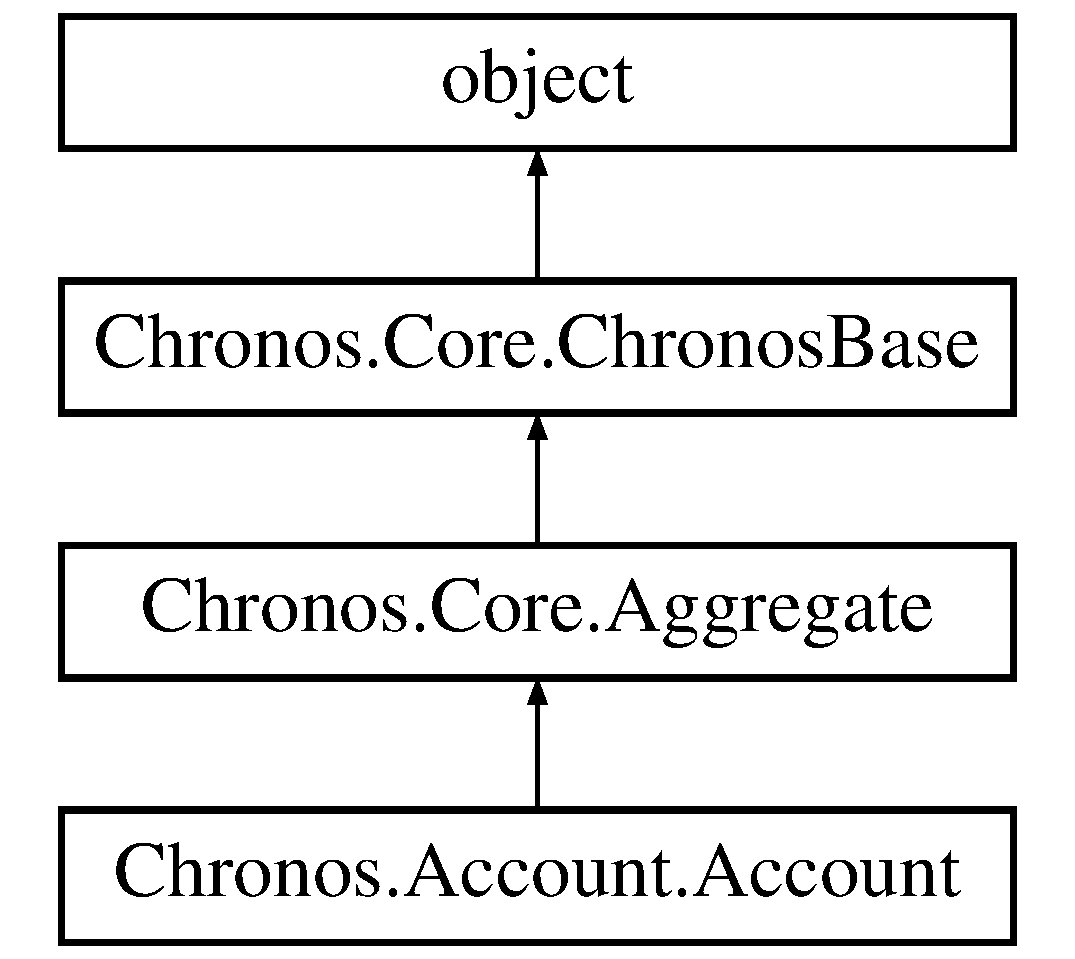
\includegraphics[height=4.000000cm]{classChronos_1_1Account_1_1Account}
\end{center}
\end{figure}
\subsection*{Public Member Functions}
\begin{DoxyCompactItemize}
\item 
def {\bfseries Is\+Valid} (self)\hypertarget{classChronos_1_1Account_1_1Account_a98e3d24098949e54f7b0abda843e6423}{}\label{classChronos_1_1Account_1_1Account_a98e3d24098949e54f7b0abda843e6423}

\end{DoxyCompactItemize}
\subsection*{Static Public Attributes}
\begin{DoxyCompactItemize}
\item 
{\bfseries Proto} = \hyperlink{classChronos_1_1Account_1_1Account}{Account}\hypertarget{classChronos_1_1Account_1_1Account_a522a6a80da72eabdd5cb25b4a3836277}{}\label{classChronos_1_1Account_1_1Account_a522a6a80da72eabdd5cb25b4a3836277}

\item 
string {\bfseries Index\+Key} = \textquotesingle{}\{owner\}\textquotesingle{}\hypertarget{classChronos_1_1Account_1_1Account_ab62a2993fac978c0755f74ca99ce026b}{}\label{classChronos_1_1Account_1_1Account_ab62a2993fac978c0755f74ca99ce026b}

\end{DoxyCompactItemize}
\subsection*{Additional Inherited Members}


The documentation for this class was generated from the following file\+:\begin{DoxyCompactItemize}
\item 
Chronos/Account.\+py\end{DoxyCompactItemize}

\hypertarget{classChronos_1_1Account_1_1CreateEvent}{}\section{Chronos.\+Account.\+Create\+Event Class Reference}
\label{classChronos_1_1Account_1_1CreateEvent}\index{Chronos.\+Account.\+Create\+Event@{Chronos.\+Account.\+Create\+Event}}
Inheritance diagram for Chronos.\+Account.\+Create\+Event\+:\begin{figure}[H]
\begin{center}
\leavevmode
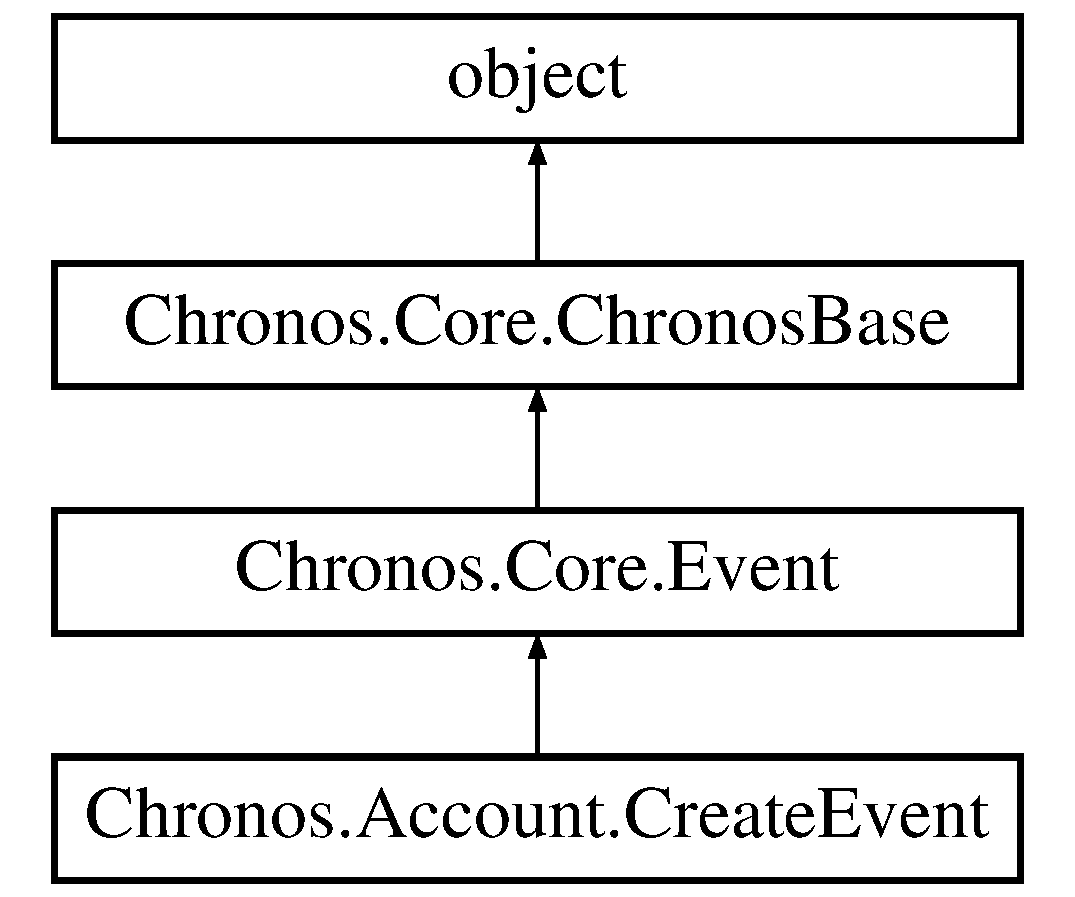
\includegraphics[height=4.000000cm]{classChronos_1_1Account_1_1CreateEvent}
\end{center}
\end{figure}
\subsection*{Public Member Functions}
\begin{DoxyCompactItemize}
\item 
def {\bfseries Raise\+For} (self, aggregate)\hypertarget{classChronos_1_1Account_1_1CreateEvent_a4f6af743e40040061e3dc2f35e51ecb9}{}\label{classChronos_1_1Account_1_1CreateEvent_a4f6af743e40040061e3dc2f35e51ecb9}

\end{DoxyCompactItemize}
\subsection*{Static Public Attributes}
\begin{DoxyCompactItemize}
\item 
{\bfseries Aggregate} = \hyperlink{classChronos_1_1Account_1_1Account}{Account}\hypertarget{classChronos_1_1Account_1_1CreateEvent_ae2395ebb0279d2796d2dd686498f85ef}{}\label{classChronos_1_1Account_1_1CreateEvent_ae2395ebb0279d2796d2dd686498f85ef}

\item 
{\bfseries Proto} = \hyperlink{classChronos_1_1Account_1_1CreateEvent}{Create\+Event}\hypertarget{classChronos_1_1Account_1_1CreateEvent_aafbdf5c85611fc863f0906d59e3a7083}{}\label{classChronos_1_1Account_1_1CreateEvent_aafbdf5c85611fc863f0906d59e3a7083}

\end{DoxyCompactItemize}
\subsection*{Additional Inherited Members}


The documentation for this class was generated from the following file\+:\begin{DoxyCompactItemize}
\item 
Chronos/Account.\+py\end{DoxyCompactItemize}

\hypertarget{classChronos_1_1Account_1_1DepositEvent}{}\section{Chronos.\+Account.\+Deposit\+Event Class Reference}
\label{classChronos_1_1Account_1_1DepositEvent}\index{Chronos.\+Account.\+Deposit\+Event@{Chronos.\+Account.\+Deposit\+Event}}
Inheritance diagram for Chronos.\+Account.\+Deposit\+Event\+:\begin{figure}[H]
\begin{center}
\leavevmode
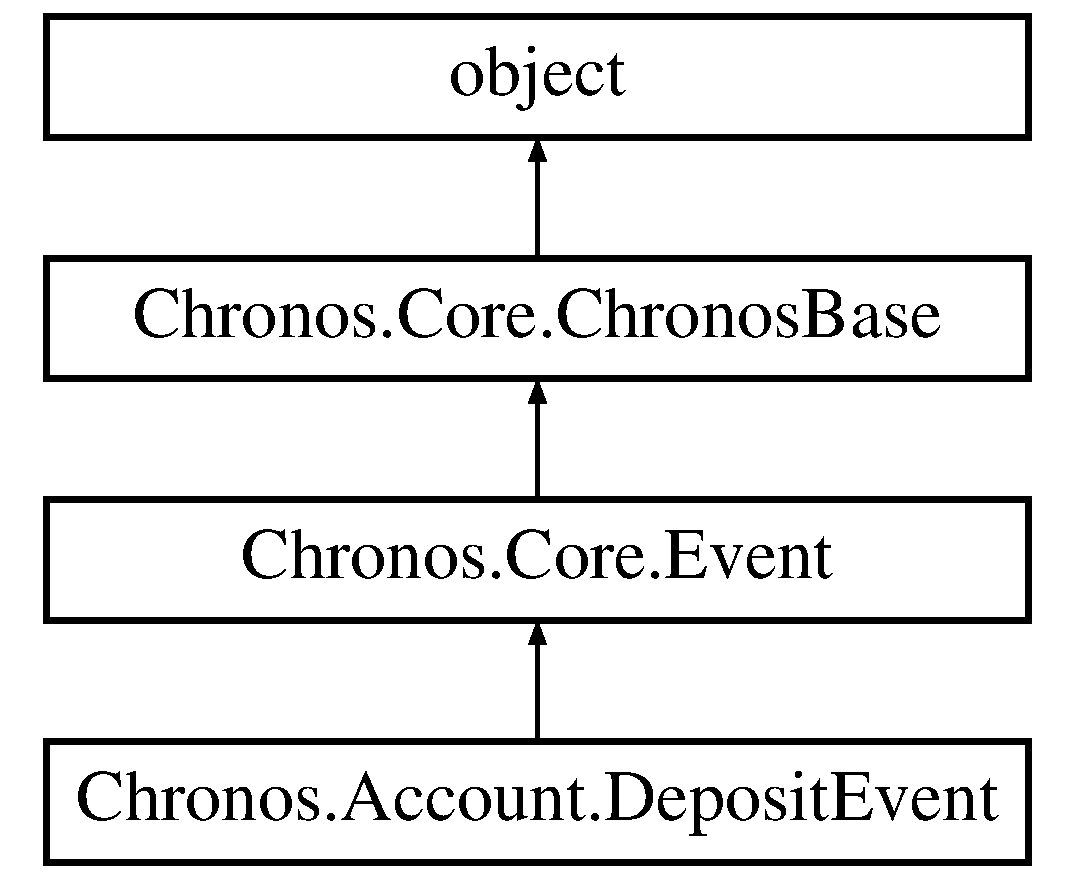
\includegraphics[height=4.000000cm]{classChronos_1_1Account_1_1DepositEvent}
\end{center}
\end{figure}
\subsection*{Public Member Functions}
\begin{DoxyCompactItemize}
\item 
def {\bfseries Raise\+For} (self, aggregate)\hypertarget{classChronos_1_1Account_1_1DepositEvent_a8788bc61a88d96dc1ae62cff017f5dab}{}\label{classChronos_1_1Account_1_1DepositEvent_a8788bc61a88d96dc1ae62cff017f5dab}

\end{DoxyCompactItemize}
\subsection*{Static Public Attributes}
\begin{DoxyCompactItemize}
\item 
{\bfseries Aggregate} = \hyperlink{classChronos_1_1Account_1_1Account}{Account}\hypertarget{classChronos_1_1Account_1_1DepositEvent_ac809d258297b95ed3d74ad71cfd563e2}{}\label{classChronos_1_1Account_1_1DepositEvent_ac809d258297b95ed3d74ad71cfd563e2}

\item 
{\bfseries Proto} = \hyperlink{classChronos_1_1Account_1_1DepositEvent}{Deposit\+Event}\hypertarget{classChronos_1_1Account_1_1DepositEvent_ade6577da7efe005d962f5cac596be02f}{}\label{classChronos_1_1Account_1_1DepositEvent_ade6577da7efe005d962f5cac596be02f}

\end{DoxyCompactItemize}
\subsection*{Additional Inherited Members}


The documentation for this class was generated from the following file\+:\begin{DoxyCompactItemize}
\item 
Chronos/Account.\+py\end{DoxyCompactItemize}

\hypertarget{classChronos_1_1Account_1_1WithdrawEvent}{}\section{Chronos.\+Account.\+Withdraw\+Event Class Reference}
\label{classChronos_1_1Account_1_1WithdrawEvent}\index{Chronos.\+Account.\+Withdraw\+Event@{Chronos.\+Account.\+Withdraw\+Event}}
Inheritance diagram for Chronos.\+Account.\+Withdraw\+Event\+:\begin{figure}[H]
\begin{center}
\leavevmode
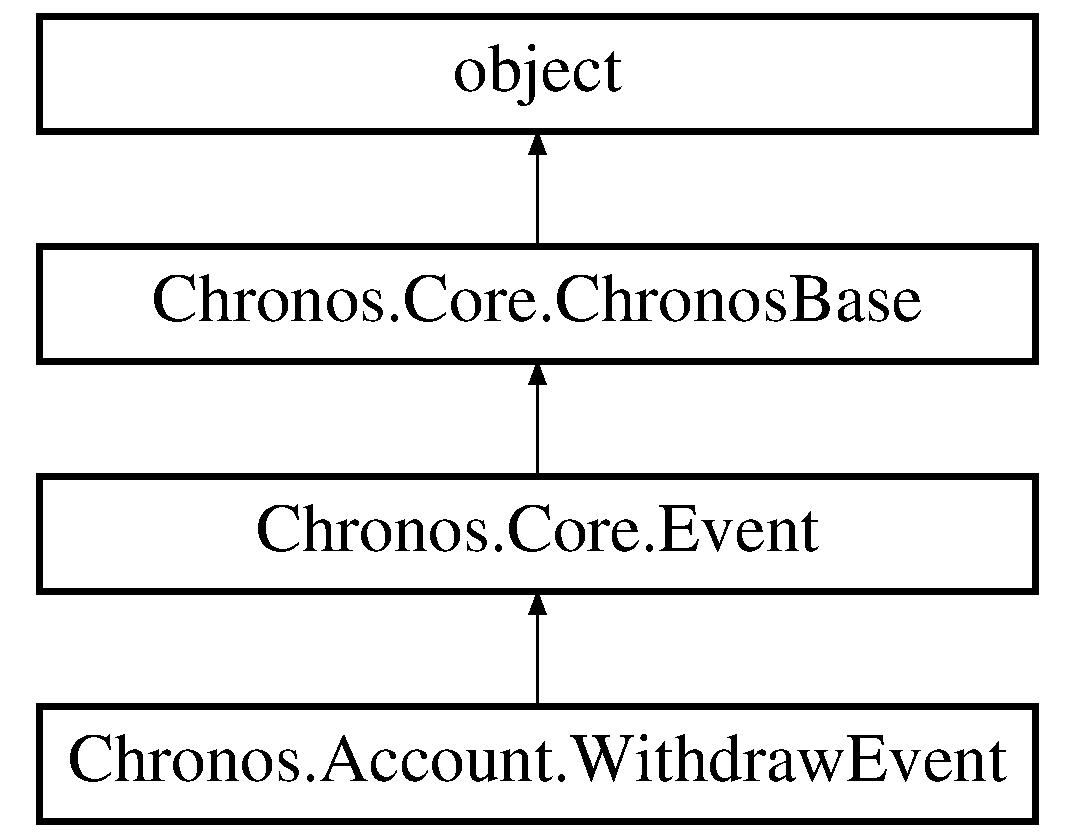
\includegraphics[height=4.000000cm]{classChronos_1_1Account_1_1WithdrawEvent}
\end{center}
\end{figure}
\subsection*{Public Member Functions}
\begin{DoxyCompactItemize}
\item 
def {\bfseries Raise\+For} (self, aggregate)\hypertarget{classChronos_1_1Account_1_1WithdrawEvent_a562004e3a174de0589605b5a7130820b}{}\label{classChronos_1_1Account_1_1WithdrawEvent_a562004e3a174de0589605b5a7130820b}

\end{DoxyCompactItemize}
\subsection*{Static Public Attributes}
\begin{DoxyCompactItemize}
\item 
{\bfseries Aggregate} = \hyperlink{classChronos_1_1Account_1_1Account}{Account}\hypertarget{classChronos_1_1Account_1_1WithdrawEvent_a38b05fdfb69a2e6cdf5458277a9343af}{}\label{classChronos_1_1Account_1_1WithdrawEvent_a38b05fdfb69a2e6cdf5458277a9343af}

\item 
{\bfseries Proto} = \hyperlink{classChronos_1_1Account_1_1WithdrawEvent}{Withdraw\+Event}\hypertarget{classChronos_1_1Account_1_1WithdrawEvent_a2f6149c36851358e326829caf1f5d077}{}\label{classChronos_1_1Account_1_1WithdrawEvent_a2f6149c36851358e326829caf1f5d077}

\end{DoxyCompactItemize}
\subsection*{Additional Inherited Members}


The documentation for this class was generated from the following file\+:\begin{DoxyCompactItemize}
\item 
Chronos/Account.\+py\end{DoxyCompactItemize}

\hypertarget{classChronos_1_1Client_1_1ChronosClient}{}\section{Chronos.\+Client.\+Chronos\+Client Class Reference}
\label{classChronos_1_1Client_1_1ChronosClient}\index{Chronos.\+Client.\+Chronos\+Client@{Chronos.\+Client.\+Chronos\+Client}}
Inheritance diagram for Chronos.\+Client.\+Chronos\+Client\+:\begin{figure}[H]
\begin{center}
\leavevmode
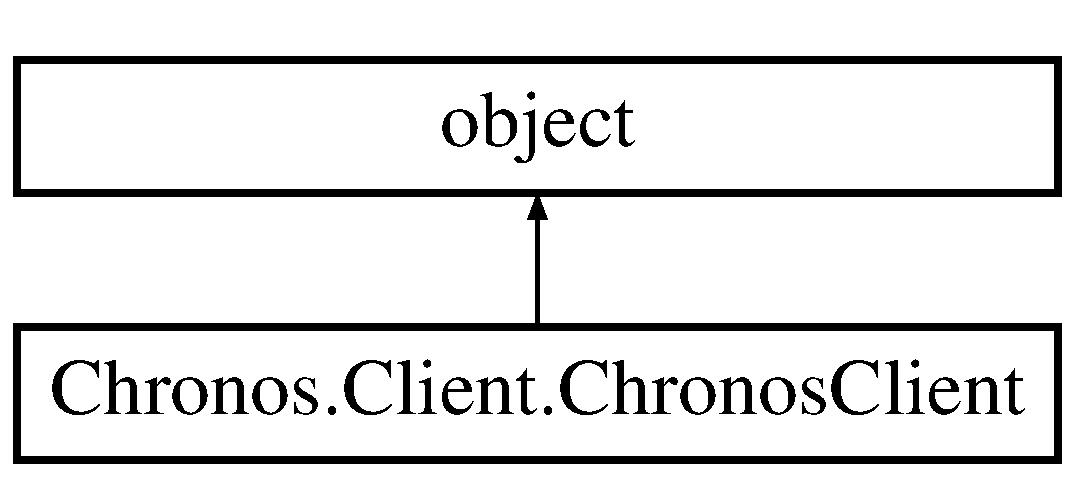
\includegraphics[height=2.000000cm]{classChronos_1_1Client_1_1ChronosClient}
\end{center}
\end{figure}
\subsection*{Public Member Functions}
\begin{DoxyCompactItemize}
\item 
def {\bfseries \+\_\+\+\_\+init\+\_\+\+\_\+} (self, aggregate\+Proto\+Class, callback=None, error\+Callback=None, management\+Callback=None, infrastructure\+Provider=None, kwargs)
\item 
def {\bfseries Connect} (self)
\item 
def {\bfseries Disconnect} (self)
\item 
def {\bfseries Dispose} (self)
\item 
def \hyperlink{group__Chronos_gae5a664ef1c7bf294b17376794264699f}{Type\+Of} (self, event\+Class)
\begin{DoxyCompactList}\small\item\em Returns the stringified type of the provided event class. \end{DoxyCompactList}\item 
def \hyperlink{group__Chronos_ga73356a0cabbb65e5ee84927e98e66b18}{Parse\+Aggregate} (self, aggregate\+Proto)
\begin{DoxyCompactList}\small\item\em Parses the provided Aggregate\+Proto instance into an instance of Aggregate\+Response for easier client-\/side use. \end{DoxyCompactList}\item 
def \hyperlink{group__Chronos_gade70bdac06e41607144ef2a0fb7a3e36}{Parse\+Event\+Response} (self, event\+Proto)
\begin{DoxyCompactList}\small\item\em Parses the provided Event\+Proto instance into an instance of Event\+Response for easier client-\/side use. \end{DoxyCompactList}\item 
def {\bfseries Register} (self)
\item 
def \hyperlink{group__Chronos_ga6cae4fd381b0282b2aa5820b3d0f6266}{Check\+Status} (self)
\begin{DoxyCompactList}\small\item\em Retrieves the Registration status of the client\textquotesingle{}s Aggregate from Chronos. \end{DoxyCompactList}\item 
def {\bfseries Unregister} (self)
\item 
def {\bfseries Raise\+Event} (self, event, aggregate\+Id=0)
\item 
def {\bfseries Raise\+Event\+With\+Tag} (self, tag, event, aggregate\+Id=0, tag\+Expiration=0)
\item 
def {\bfseries Raise\+Transaction} (self, events)
\item 
def {\bfseries Subscribe} (self, indices)
\item 
def {\bfseries Unsubscribe} (self, indices)
\item 
def {\bfseries Unsubscribe\+All} (self)
\item 
def {\bfseries Get\+All\+Aggregates} (self)
\item 
def {\bfseries Get\+Aggregate\+By\+Id} (self, aggregate\+Id)
\item 
def {\bfseries Get\+Aggregates\+By\+Index} (self, kwargs)
\item 
def {\bfseries Get\+Aggregate\+By\+Tag} (self, aggregate\+Id, tag)
\item 
def {\bfseries Get\+All\+Tags} (self)
\end{DoxyCompactItemize}
\subsection*{Static Public Member Functions}
\begin{DoxyCompactItemize}
\item 
def \hyperlink{group__Chronos_gafdce0107a1a368f4f4f7e7c9b084fc0c}{Parse\+Event} (event\+Class, event\+Proto)
\begin{DoxyCompactList}\small\item\em Parses the provided Event\+Proto instance into an instance of the provided event protobuf entity. \end{DoxyCompactList}\end{DoxyCompactItemize}
\subsection*{Public Attributes}
\begin{DoxyCompactItemize}
\item 
{\bfseries client\+Id}
\item 
{\bfseries aggregate\+Proto\+Class}
\item 
{\bfseries aggregate\+Name}
\item 
{\bfseries callback}
\item 
{\bfseries error\+Callback}
\item 
{\bfseries management\+Callback}
\item 
{\bfseries success\+Processor}
\item 
{\bfseries failure\+Processor}
\item 
{\bfseries management\+Processor}
\item 
{\bfseries subscription\+Manager}
\item 
{\bfseries service\+Proxy\+Manager}
\item 
{\bfseries client}
\end{DoxyCompactItemize}
\subsection*{Static Public Attributes}
\begin{DoxyCompactItemize}
\item 
tuple {\bfseries Event\+Types} = ()
\item 
string {\bfseries Service\+Name} = \textquotesingle{}Chronos\textquotesingle{}
\end{DoxyCompactItemize}


The documentation for this class was generated from the following file\+:\begin{DoxyCompactItemize}
\item 
Chronos/Client.\+py\end{DoxyCompactItemize}

\hypertarget{classChronos_1_1Client_1_1ChronosClientException}{}\section{Chronos.\+Client.\+Chronos\+Client\+Exception Class Reference}
\label{classChronos_1_1Client_1_1ChronosClientException}\index{Chronos.\+Client.\+Chronos\+Client\+Exception@{Chronos.\+Client.\+Chronos\+Client\+Exception}}
Inheritance diagram for Chronos.\+Client.\+Chronos\+Client\+Exception\+:\begin{figure}[H]
\begin{center}
\leavevmode
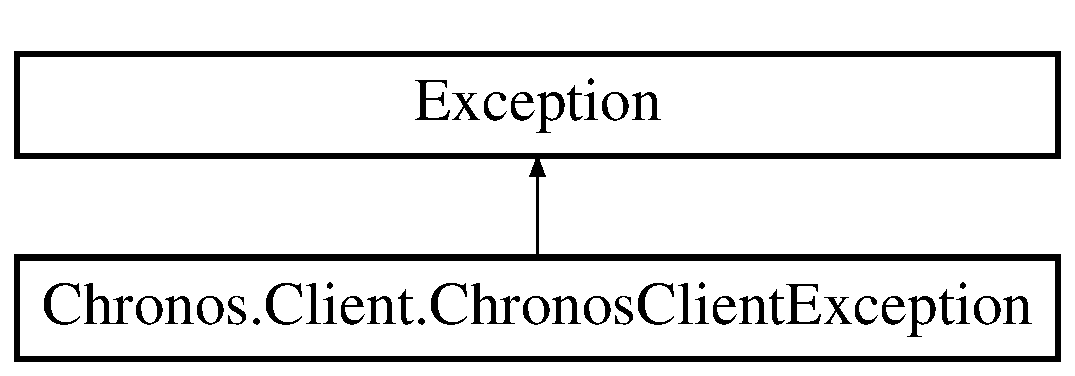
\includegraphics[height=2.000000cm]{classChronos_1_1Client_1_1ChronosClientException}
\end{center}
\end{figure}


The documentation for this class was generated from the following file\+:\begin{DoxyCompactItemize}
\item 
Chronos/Client.\+py\end{DoxyCompactItemize}

\hypertarget{classChronos_1_1Client_1_1ChronosTransactionItem}{}\section{Chronos.\+Client.\+Chronos\+Transaction\+Item Class Reference}
\label{classChronos_1_1Client_1_1ChronosTransactionItem}\index{Chronos.\+Client.\+Chronos\+Transaction\+Item@{Chronos.\+Client.\+Chronos\+Transaction\+Item}}


Represents a single action that should take place as part of an atomic Chronos transaction.  


Inheritance diagram for Chronos.\+Client.\+Chronos\+Transaction\+Item\+:\begin{figure}[H]
\begin{center}
\leavevmode
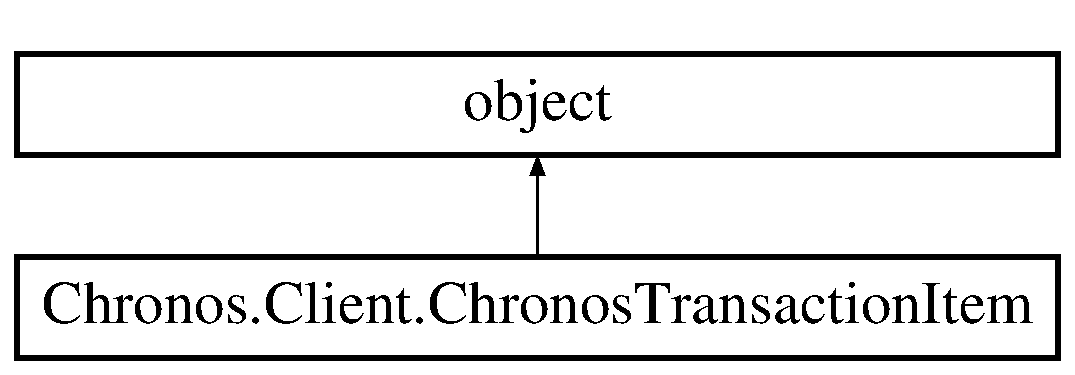
\includegraphics[height=2.000000cm]{classChronos_1_1Client_1_1ChronosTransactionItem}
\end{center}
\end{figure}
\subsection*{Public Member Functions}
\begin{DoxyCompactItemize}
\item 
def {\bfseries \+\_\+\+\_\+init\+\_\+\+\_\+} (self, event, aggregate\+Id=0, tag=None, tag\+Expiration=0)
\end{DoxyCompactItemize}
\subsection*{Public Attributes}
\begin{DoxyCompactItemize}
\item 
{\bfseries event}
\item 
{\bfseries aggregate\+Id}
\item 
{\bfseries tag}
\item 
{\bfseries tag\+Expiration}
\end{DoxyCompactItemize}


\subsection{Detailed Description}
Represents a single action that should take place as part of an atomic Chronos transaction. 

The documentation for this class was generated from the following file\+:\begin{DoxyCompactItemize}
\item 
Chronos/Client.\+py\end{DoxyCompactItemize}

\hypertarget{classChronos_1_1Client_1_1SubscriptionManager}{}\section{Chronos.\+Client.\+Subscription\+Manager Class Reference}
\label{classChronos_1_1Client_1_1SubscriptionManager}\index{Chronos.\+Client.\+Subscription\+Manager@{Chronos.\+Client.\+Subscription\+Manager}}


Handles subscription logic for Chronos Client instances.  


Inheritance diagram for Chronos.\+Client.\+Subscription\+Manager\+:\begin{figure}[H]
\begin{center}
\leavevmode
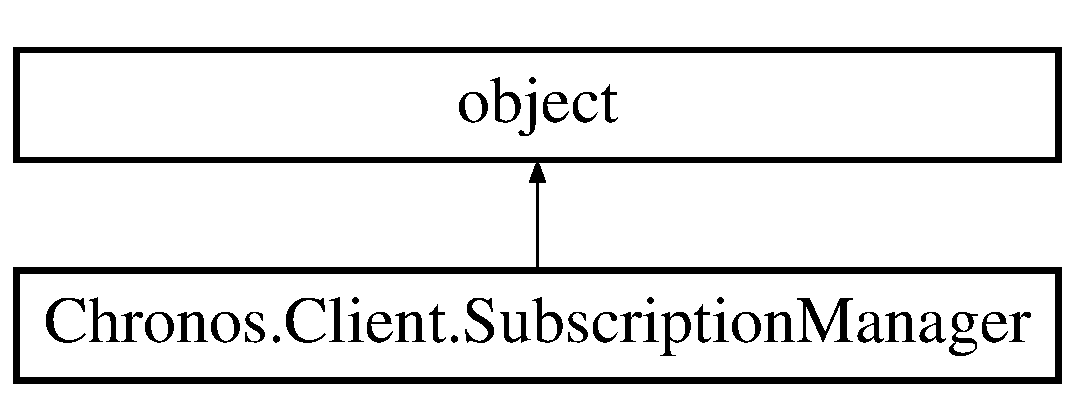
\includegraphics[height=2.000000cm]{classChronos_1_1Client_1_1SubscriptionManager}
\end{center}
\end{figure}
\subsection*{Public Member Functions}
\begin{DoxyCompactItemize}
\item 
def \hyperlink{group__Chronos_ga17b0ece7d5be132801d46977ffac3bcc}{\+\_\+\+\_\+init\+\_\+\+\_\+} (self, event\+Store, aggregate\+Class, success\+Callback, failure\+Callback, management\+Callback)
\begin{DoxyCompactList}\small\item\em Initializes a new \hyperlink{classChronos_1_1Client_1_1SubscriptionManager}{Subscription\+Manager} instance. \end{DoxyCompactList}\item 
def \hyperlink{group__Chronos_gae21ba8cca5cb7ffe3085e39b9ef18945}{Subscribe\+For\+Unified\+Updates} (self)
\begin{DoxyCompactList}\small\item\em Subscribes {\ttfamily event\+Store} for Chronos failure and management messages. \end{DoxyCompactList}\item 
def \hyperlink{group__Chronos_ga4d1b5c99ac9d282cd4a5b39f5ace3615}{Unsubscribe\+For\+Unified\+Updates} (self)
\begin{DoxyCompactList}\small\item\em Unsubscribes for unified updates. \end{DoxyCompactList}\item 
def \hyperlink{group__Chronos_ga83af8c47b1d510ea2aa638680b9304ed}{Subscribe} (self, indices)
\begin{DoxyCompactList}\small\item\em Subscribes for messages for Aggregate instances that match the fields provided in {\ttfamily indices}. \end{DoxyCompactList}\item 
def \hyperlink{group__Chronos_ga115103720707b543e309432166332e1d}{Unsubscribe} (self, indices)
\begin{DoxyCompactList}\small\item\em Unsubscribes for messages previously registered by Subscribe. \end{DoxyCompactList}\item 
def \hyperlink{group__Chronos_gaef0709e91993c04a0e27eb158e4e8514}{Unsubscribe\+All} (self)
\begin{DoxyCompactList}\small\item\em Unsubscribes for all updates previously registered by Subscribe. \end{DoxyCompactList}\item 
def \hyperlink{group__Chronos_ga8c7e61cf993d0b145642c632f064921d}{Resubscribe} (self, indexed\+Attributes)
\begin{DoxyCompactList}\small\item\em Processes the provided {\ttfamily indexed\+Attributes} and determines if currently registered subscriptions have to be renewed. \end{DoxyCompactList}\end{DoxyCompactItemize}
\subsection*{Public Attributes}
\begin{DoxyCompactItemize}
\item 
{\bfseries event\+Store}
\item 
{\bfseries aggregate\+Name}
\item 
{\bfseries success\+Callback}
\item 
{\bfseries failure\+Callback}
\item 
{\bfseries management\+Callback}
\item 
{\bfseries subscription\+Prefix}
\item 
{\bfseries failure\+Channel}
\item 
{\bfseries management\+Channel}
\item 
{\bfseries subscriptions}
\item 
{\bfseries lock}
\item 
{\bfseries indexed\+Attributes}
\end{DoxyCompactItemize}


\subsection{Detailed Description}
Handles subscription logic for Chronos Client instances. 

\hyperlink{classChronos_1_1Client_1_1SubscriptionManager}{Subscription\+Manager} is primarily responsible for ensuring that subscriptions remain consistent through Redis failures and Chronos index schema divergence. 

The documentation for this class was generated from the following file\+:\begin{DoxyCompactItemize}
\item 
Chronos/Client.\+py\end{DoxyCompactItemize}

\hypertarget{classChronos_1_1Client_1_1TagNotFound}{}\section{Chronos.\+Client.\+Tag\+Not\+Found Class Reference}
\label{classChronos_1_1Client_1_1TagNotFound}\index{Chronos.\+Client.\+Tag\+Not\+Found@{Chronos.\+Client.\+Tag\+Not\+Found}}


Raised when a requested tag was not known by the Chronos service.  


Inheritance diagram for Chronos.\+Client.\+Tag\+Not\+Found\+:\begin{figure}[H]
\begin{center}
\leavevmode
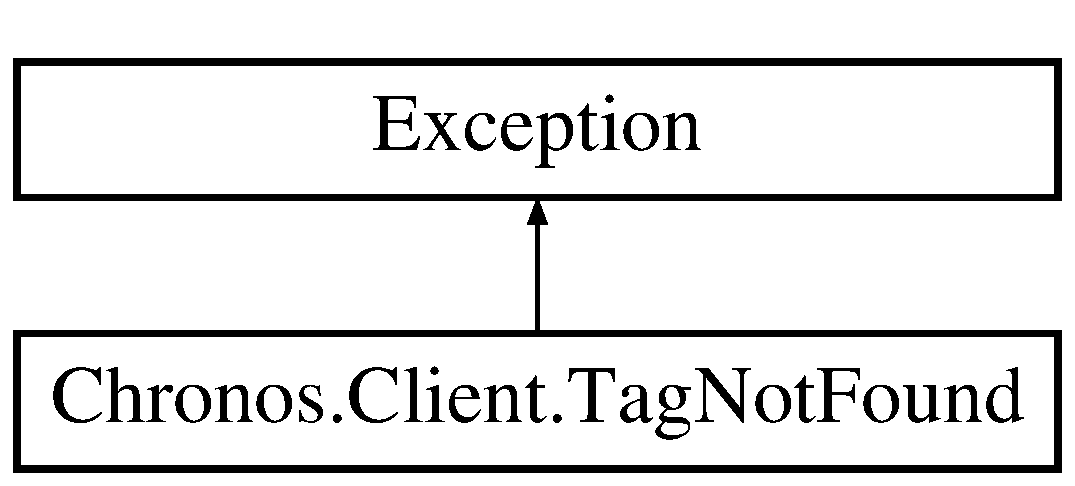
\includegraphics[height=2.000000cm]{classChronos_1_1Client_1_1TagNotFound}
\end{center}
\end{figure}


\subsection{Detailed Description}
Raised when a requested tag was not known by the Chronos service. 

This Exception exists to differentiate service failures from missing tags. 

The documentation for this class was generated from the following file\+:\begin{DoxyCompactItemize}
\item 
Chronos/Client.\+py\end{DoxyCompactItemize}

\hypertarget{classChronos_1_1Core_1_1Aggregate}{}\section{Chronos.\+Core.\+Aggregate Class Reference}
\label{classChronos_1_1Core_1_1Aggregate}\index{Chronos.\+Core.\+Aggregate@{Chronos.\+Core.\+Aggregate}}


The public \hyperlink{classChronos_1_1Core_1_1Aggregate}{Aggregate} base class.  


Inheritance diagram for Chronos.\+Core.\+Aggregate\+:\begin{figure}[H]
\begin{center}
\leavevmode
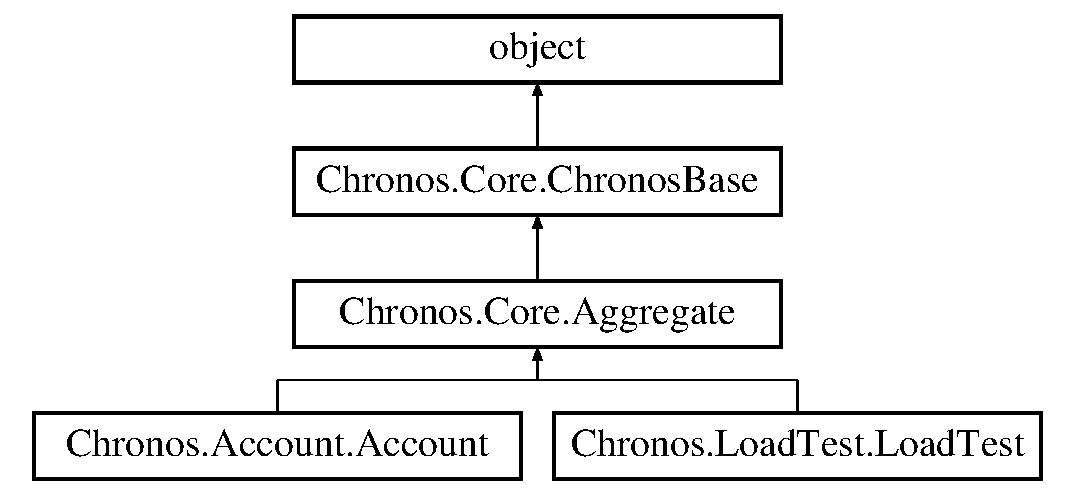
\includegraphics[height=4.000000cm]{classChronos_1_1Core_1_1Aggregate}
\end{center}
\end{figure}
\subsection*{Public Member Functions}
\begin{DoxyCompactItemize}
\item 
def {\bfseries \+\_\+\+\_\+init\+\_\+\+\_\+} (self, aggregate\+Id, version, expiration)
\item 
def {\bfseries Is\+Valid} (self)
\item 
def {\bfseries Get\+Indices} (self)
\item 
def {\bfseries Has\+Diverged\+From} (self, previous\+Version)
\item 
def {\bfseries To\+Dict} (self)
\item 
def {\bfseries From\+Dict} (cls, dct)
\item 
def {\bfseries \+\_\+\+\_\+deepcopy\+\_\+\+\_\+} (self, memo)
\item 
def \hyperlink{group__Chronos_gad756f2fc68dddd2ffd3ce45ef50e6820}{\+\_\+\+\_\+getstate\+\_\+\+\_\+} (self)
\begin{DoxyCompactList}\small\item\em For queries, \hyperlink{classChronos_1_1Core_1_1Aggregate}{Aggregate} instances must be pickleable. \end{DoxyCompactList}\end{DoxyCompactItemize}
\subsection*{Public Attributes}
\begin{DoxyCompactItemize}
\item 
{\bfseries aggregate\+Id}
\item 
{\bfseries version}
\item 
{\bfseries expiration}
\item 
{\bfseries lock}
\end{DoxyCompactItemize}
\subsection*{Static Public Attributes}
\begin{DoxyCompactItemize}
\item 
int {\bfseries Cache\+Size} = 1000
\item 
int {\bfseries Expiration} = 0
\end{DoxyCompactItemize}


\subsection{Detailed Description}
The public \hyperlink{classChronos_1_1Core_1_1Aggregate}{Aggregate} base class. 

This mainly exists to connect \hyperlink{classChronos_1_1Core_1_1AggregateMeta}{Aggregate\+Meta} and \hyperlink{classChronos_1_1Core_1_1ChronosBase}{Chronos\+Base} so that the client can subclass a single class in their code. 

The documentation for this class was generated from the following file\+:\begin{DoxyCompactItemize}
\item 
Chronos/Core.\+py\end{DoxyCompactItemize}

\hypertarget{classChronos_1_1Core_1_1AggregateLogicCompiler}{}\section{Chronos.\+Core.\+Aggregate\+Logic\+Compiler Class Reference}
\label{classChronos_1_1Core_1_1AggregateLogicCompiler}\index{Chronos.\+Core.\+Aggregate\+Logic\+Compiler@{Chronos.\+Core.\+Aggregate\+Logic\+Compiler}}


Handles all operations related to \hyperlink{classChronos_1_1Core_1_1Aggregate}{Aggregate} logic compilation.  


Inheritance diagram for Chronos.\+Core.\+Aggregate\+Logic\+Compiler\+:\begin{figure}[H]
\begin{center}
\leavevmode
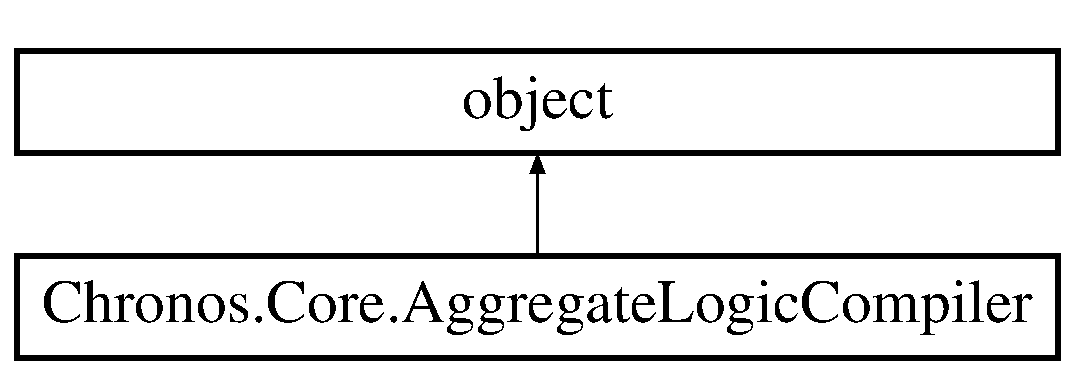
\includegraphics[height=2.000000cm]{classChronos_1_1Core_1_1AggregateLogicCompiler}
\end{center}
\end{figure}
\subsection*{Public Member Functions}
\begin{DoxyCompactItemize}
\item 
def {\bfseries \+\_\+\+\_\+init\+\_\+\+\_\+} (self, event\+Store)
\item 
def \hyperlink{group__Chronos_ga751fbece3b09db34133314bfde9052f6}{Build\+Module} (self, aggregate\+Name, aggregate\+Logic)
\begin{DoxyCompactList}\small\item\em Constructs a module containing the provided aggregate\+Logic, wired to the proper Protobuf entities. \end{DoxyCompactList}\item 
def \hyperlink{group__Chronos_ga5c8b8498a50aa6157dbf12c35c09748f}{Compile} (self, aggregate\+Name, aggregate\+Logic)
\begin{DoxyCompactList}\small\item\em Handles compilation and persistence of \hyperlink{classChronos_1_1Core_1_1Aggregate}{Aggregate} logic. \end{DoxyCompactList}\end{DoxyCompactItemize}
\subsection*{Static Public Member Functions}
\begin{DoxyCompactItemize}
\item 
def {\bfseries Import\+Aggregate\+Logic} (aggregate\+Name)
\end{DoxyCompactItemize}
\subsection*{Public Attributes}
\begin{DoxyCompactItemize}
\item 
{\bfseries event\+Store}
\end{DoxyCompactItemize}


\subsection{Detailed Description}
Handles all operations related to \hyperlink{classChronos_1_1Core_1_1Aggregate}{Aggregate} logic compilation. 

\hyperlink{classChronos_1_1Core_1_1Aggregate}{Aggregate} logic is compiled into Python modules that are used by Chronos\+Process. In addition, this class handles the persistence of logic versions and ids so that events from the past can be replayed without worrying about backwards compatibility while making changes. 

The documentation for this class was generated from the following file\+:\begin{DoxyCompactItemize}
\item 
Chronos/Core.\+py\end{DoxyCompactItemize}

\hypertarget{classChronos_1_1Core_1_1AggregateMeta}{}\section{Chronos.\+Core.\+Aggregate\+Meta Class Reference}
\label{classChronos_1_1Core_1_1AggregateMeta}\index{Chronos.\+Core.\+Aggregate\+Meta@{Chronos.\+Core.\+Aggregate\+Meta}}


Validates and sets up classes as proper Chronos Aggregates.  


Inheritance diagram for Chronos.\+Core.\+Aggregate\+Meta\+:\begin{figure}[H]
\begin{center}
\leavevmode
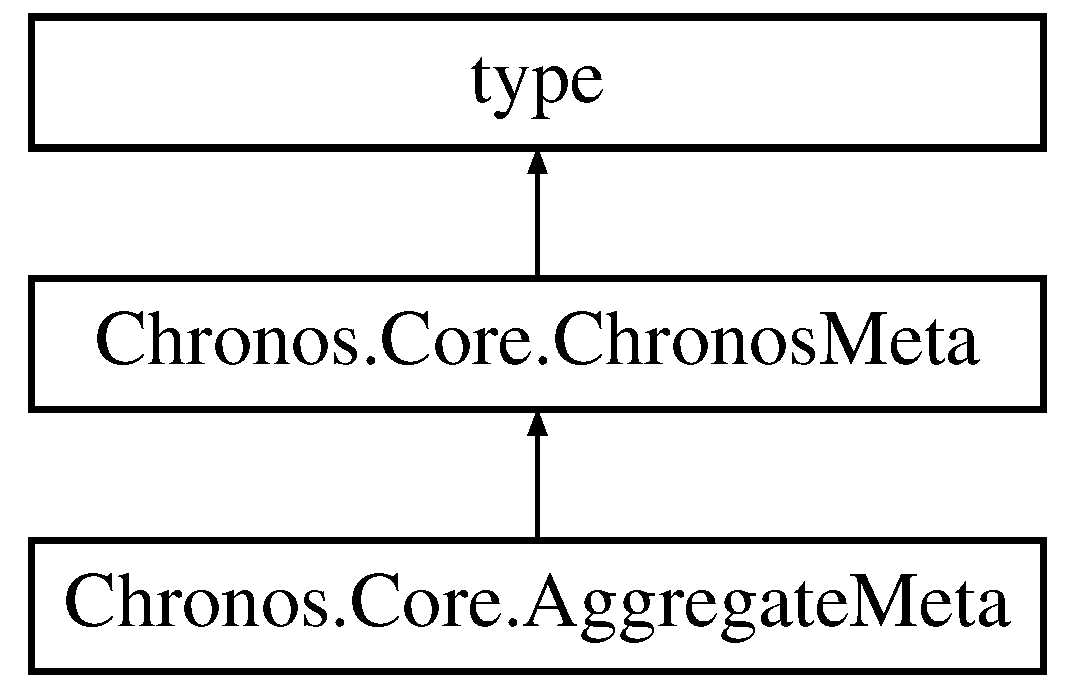
\includegraphics[height=3.000000cm]{classChronos_1_1Core_1_1AggregateMeta}
\end{center}
\end{figure}
\subsection*{Public Member Functions}
\begin{DoxyCompactItemize}
\item 
def {\bfseries \+\_\+\+\_\+init\+\_\+\+\_\+} (cls, name, bases, dct)
\end{DoxyCompactItemize}
\subsection*{Public Attributes}
\begin{DoxyCompactItemize}
\item 
{\bfseries Dependencies}
\item 
{\bfseries Indexed\+Attributes}
\end{DoxyCompactItemize}


\subsection{Detailed Description}
Validates and sets up classes as proper Chronos Aggregates. 

Defining an \hyperlink{classChronos_1_1Core_1_1AggregateMeta}{Aggregate\+Meta} will enforce that only a single \hyperlink{classChronos_1_1Core_1_1AggregateMeta}{Aggregate\+Meta} exists in the current module, and then will modify the module in preparation for event registration.

In addition, if an Index\+Key property exists on the class, it will be validated against the underlying protobuf class members, and class members will be set accordingly on the \hyperlink{classChronos_1_1Core_1_1Aggregate}{Aggregate} class.

For example, consider the following Protobuf message\+: 
\begin{DoxyCode}
1 message AProtobufMessage \{
2     optional string firmName = 1;
3     optional string infoSysName = 2;
4     optional string traderAcronym = 3;
5 \}
\end{DoxyCode}


If the following module is declared\+: 
\begin{DoxyCode}
1 \textcolor{keyword}{class }AnIndex(ChronosIndex):
2     firmName = Column(String)
3     infoSysName = Column(String)
4     constraints = [UniqueConstraint(\textcolor{stringliteral}{'firmName'}, \textcolor{stringliteral}{'infoSysName'}, name=\textcolor{stringliteral}{'ux\_1'})]
5 
6 \textcolor{keyword}{class }AnAggregate(Aggregate):
7     Proto = AProtobufMessage
8     Index = AnIndex
\end{DoxyCode}


Then Chronos will automatically generate the necessary metadata to allow for querying of An\+Aggregate by firm\+Name and info\+Sys\+Name. The provided unique constraint will also be enforced for both aggregate creation and modification. 

The documentation for this class was generated from the following file\+:\begin{DoxyCompactItemize}
\item 
Chronos/Core.\+py\end{DoxyCompactItemize}

\hypertarget{classChronos_1_1Core_1_1AggregateRepository}{}\section{Chronos.\+Core.\+Aggregate\+Repository Class Reference}
\label{classChronos_1_1Core_1_1AggregateRepository}\index{Chronos.\+Core.\+Aggregate\+Repository@{Chronos.\+Core.\+Aggregate\+Repository}}


The in-\/memory representation of the current state of all aggregates within an aggregate root.  


Inheritance diagram for Chronos.\+Core.\+Aggregate\+Repository\+:\begin{figure}[H]
\begin{center}
\leavevmode
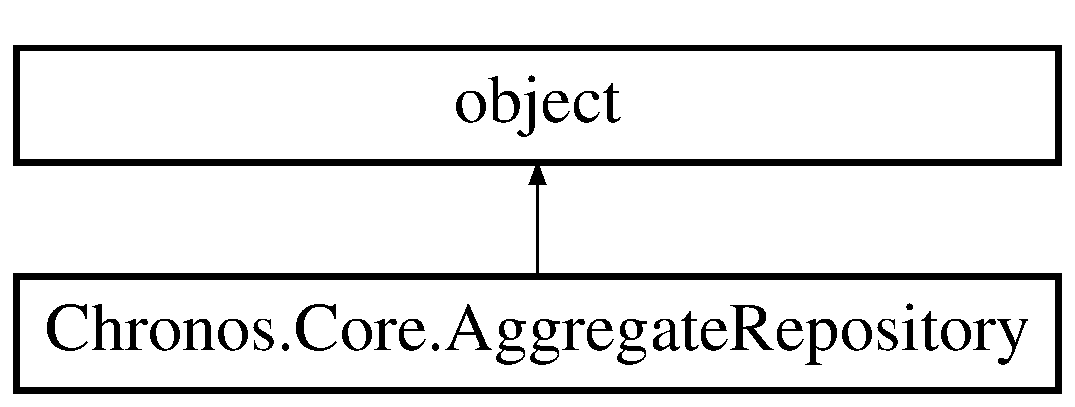
\includegraphics[height=2.000000cm]{classChronos_1_1Core_1_1AggregateRepository}
\end{center}
\end{figure}
\subsection*{Public Member Functions}
\begin{DoxyCompactItemize}
\item 
def {\bfseries \+\_\+\+\_\+init\+\_\+\+\_\+} (self, aggregate\+Class, index\+Store, event\+Store)
\item 
def {\bfseries Begin} (self)
\item 
def {\bfseries Commit} (self)
\item 
def {\bfseries Rollback} (self)
\item 
def \hyperlink{group__Chronos_ga631476634e37f9961dba1bb160bb9ee5}{Create} (self)
\begin{DoxyCompactList}\small\item\em Creates a new uninitialized aggregate, permanently incrementing the aggregate root id in the event store. \end{DoxyCompactList}\item 
def \hyperlink{group__Chronos_ga8b9bae0731e091c9f2a79803149f5449}{Get} (self, aggregate\+Id)
\begin{DoxyCompactList}\small\item\em Retrieves a single aggregate snaphost using the provided id. \end{DoxyCompactList}\item 
def \hyperlink{group__Chronos_ga21a75e7e033c6cf88ac47d6525f8c991}{Atomic\+Get} (self, aggregate\+Id)
\begin{DoxyCompactList}\small\item\em Retrieves a single aggregate snapshot for dependency acquisition. \end{DoxyCompactList}\item 
def \hyperlink{group__Chronos_ga5034ab423a49b011e6f90460ddd4e70e}{Emplace} (self, aggregate)
\begin{DoxyCompactList}\small\item\em Replaces an existing aggregate with its new state. \end{DoxyCompactList}\item 
def {\bfseries Get\+Event\+Persistence\+Checkpoint} (self)
\item 
def \hyperlink{group__Chronos_gac9cde7c90df6d8e1d0c0166cfa87358c}{Get\+All} (self)
\begin{DoxyCompactList}\small\item\em Retrieves all aggregate snapshots available in the event store and returns them. \end{DoxyCompactList}\item 
def \hyperlink{group__Chronos_ga4abb70024e82d3dca4f92c634bdc4bfd}{Get\+From\+Index} (self, kwargs)
\begin{DoxyCompactList}\small\item\em Retrieves all aggregates that satisfy the provided index contraints. \end{DoxyCompactList}\item 
def {\bfseries Get\+Tag} (self, aggregate\+Id, tag)
\end{DoxyCompactItemize}
\subsection*{Public Attributes}
\begin{DoxyCompactItemize}
\item 
{\bfseries aggregate\+Class}
\item 
{\bfseries index\+Store}
\item 
{\bfseries event\+Store}
\item 
{\bfseries repository}
\item 
{\bfseries transaction\+Repository}
\item 
{\bfseries transaction\+Lock}
\item 
{\bfseries transaction\+Event}
\end{DoxyCompactItemize}


\subsection{Detailed Description}
The in-\/memory representation of the current state of all aggregates within an aggregate root. 

\hyperlink{classChronos_1_1Core_1_1AggregateRepository}{Aggregate\+Repository} handles interaction with an event store to return aggregates to the user. 

The documentation for this class was generated from the following file\+:\begin{DoxyCompactItemize}
\item 
Chronos/Core.\+py\end{DoxyCompactItemize}

\hypertarget{classChronos_1_1Core_1_1ChronosBase}{}\section{Chronos.\+Core.\+Chronos\+Base Class Reference}
\label{classChronos_1_1Core_1_1ChronosBase}\index{Chronos.\+Core.\+Chronos\+Base@{Chronos.\+Core.\+Chronos\+Base}}


Provides common functionality for Chronos base classes, \hyperlink{classChronos_1_1Core_1_1Aggregate}{Aggregate} and \hyperlink{classChronos_1_1Core_1_1Event}{Event}.  


Inheritance diagram for Chronos.\+Core.\+Chronos\+Base\+:\begin{figure}[H]
\begin{center}
\leavevmode
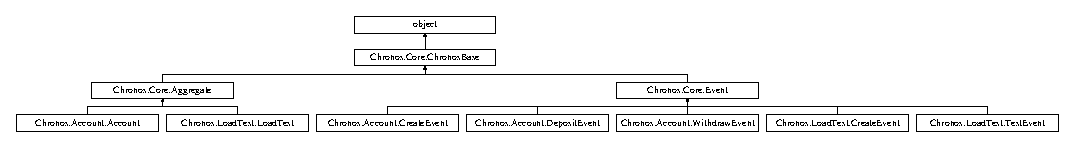
\includegraphics[height=1.545894cm]{classChronos_1_1Core_1_1ChronosBase}
\end{center}
\end{figure}
\subsection*{Public Member Functions}
\begin{DoxyCompactItemize}
\item 
def {\bfseries \+\_\+\+\_\+init\+\_\+\+\_\+} (self)
\end{DoxyCompactItemize}
\subsection*{Public Attributes}
\begin{DoxyCompactItemize}
\item 
{\bfseries proto}
\end{DoxyCompactItemize}


\subsection{Detailed Description}
Provides common functionality for Chronos base classes, \hyperlink{classChronos_1_1Core_1_1Aggregate}{Aggregate} and \hyperlink{classChronos_1_1Core_1_1Event}{Event}. 

Any subclass of \hyperlink{classChronos_1_1Core_1_1ChronosBase}{Chronos\+Base} will automatically have all of the same properties as its underlying protobuf class. 

The documentation for this class was generated from the following file\+:\begin{DoxyCompactItemize}
\item 
Chronos/Core.\+py\end{DoxyCompactItemize}

\hypertarget{classChronos_1_1Core_1_1ChronosCoreException}{}\section{Chronos.\+Core.\+Chronos\+Core\+Exception Class Reference}
\label{classChronos_1_1Core_1_1ChronosCoreException}\index{Chronos.\+Core.\+Chronos\+Core\+Exception@{Chronos.\+Core.\+Chronos\+Core\+Exception}}


An Exception indicating that Chronos has encountered an error from which it is unable to recover.  


Inheritance diagram for Chronos.\+Core.\+Chronos\+Core\+Exception\+:\begin{figure}[H]
\begin{center}
\leavevmode
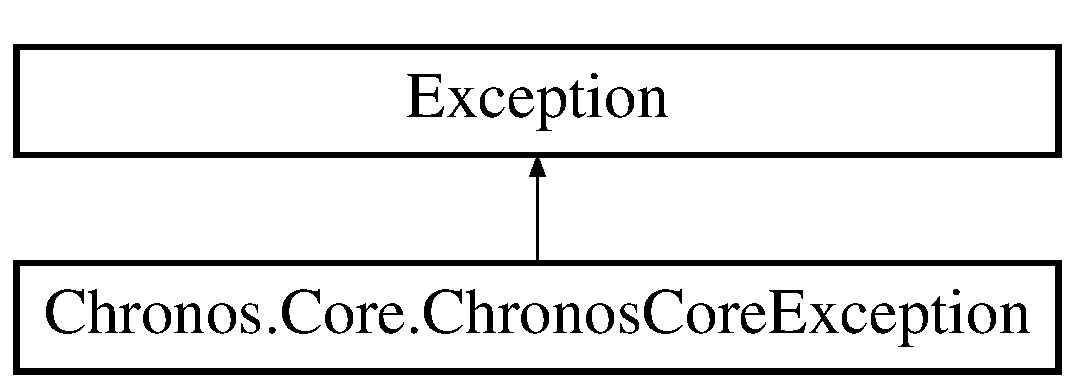
\includegraphics[height=2.000000cm]{classChronos_1_1Core_1_1ChronosCoreException}
\end{center}
\end{figure}


\subsection{Detailed Description}
An Exception indicating that Chronos has encountered an error from which it is unable to recover. 

This Exception should only be thrown if the A\+PI is being used in an incorrect manner. 

The documentation for this class was generated from the following file\+:\begin{DoxyCompactItemize}
\item 
Chronos/Core.\+py\end{DoxyCompactItemize}

\hypertarget{classChronos_1_1Core_1_1ChronosCoreProvider}{}\section{Chronos.\+Core.\+Chronos\+Core\+Provider Class Reference}
\label{classChronos_1_1Core_1_1ChronosCoreProvider}\index{Chronos.\+Core.\+Chronos\+Core\+Provider@{Chronos.\+Core.\+Chronos\+Core\+Provider}}


A factory class that provides implementations of core Chronos functionality to other modules.  


Inheritance diagram for Chronos.\+Core.\+Chronos\+Core\+Provider\+:\begin{figure}[H]
\begin{center}
\leavevmode
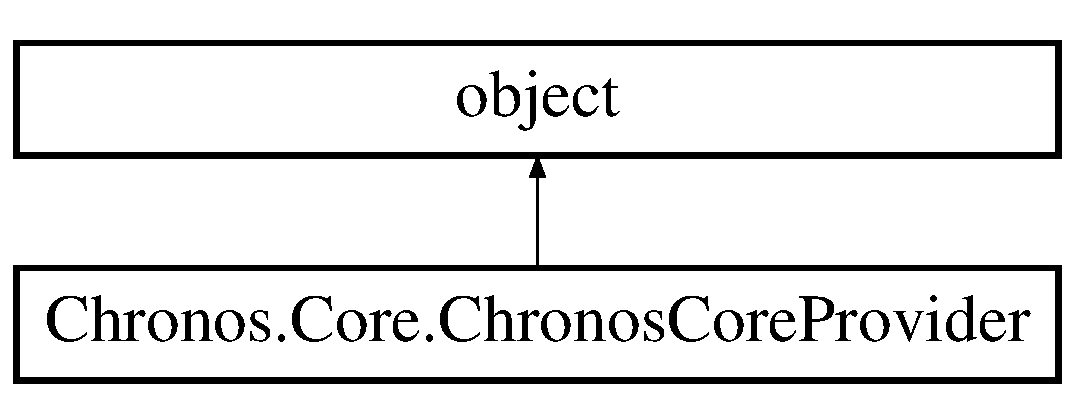
\includegraphics[height=2.000000cm]{classChronos_1_1Core_1_1ChronosCoreProvider}
\end{center}
\end{figure}
\subsection*{Public Member Functions}
\begin{DoxyCompactItemize}
\item 
def {\bfseries \+\_\+\+\_\+init\+\_\+\+\_\+} (self, aggregate\+Class)
\item 
def {\bfseries Dispose} (self)
\item 
def {\bfseries Get\+Index\+Store} (self)
\item 
def {\bfseries Get\+Repository} (self)
\item 
def {\bfseries Get\+Processor} (self)
\end{DoxyCompactItemize}
\subsection*{Public Attributes}
\begin{DoxyCompactItemize}
\item 
{\bfseries infrastructure\+Provider}
\item 
{\bfseries index\+Store}
\item 
{\bfseries event\+Store}
\item 
{\bfseries aggregate\+Repository}
\item 
{\bfseries event\+Processor}
\end{DoxyCompactItemize}


\subsection{Detailed Description}
A factory class that provides implementations of core Chronos functionality to other modules. 

\begin{DoxySeeAlso}{See also}
Chronos\+::\+Gateway 
\end{DoxySeeAlso}


The documentation for this class was generated from the following file\+:\begin{DoxyCompactItemize}
\item 
Chronos/Core.\+py\end{DoxyCompactItemize}

\hypertarget{classChronos_1_1Core_1_1ChronosDeclarativeBase}{}\section{Chronos.\+Core.\+Chronos\+Declarative\+Base Class Reference}
\label{classChronos_1_1Core_1_1ChronosDeclarativeBase}\index{Chronos.\+Core.\+Chronos\+Declarative\+Base@{Chronos.\+Core.\+Chronos\+Declarative\+Base}}
Inheritance diagram for Chronos.\+Core.\+Chronos\+Declarative\+Base\+:\begin{figure}[H]
\begin{center}
\leavevmode
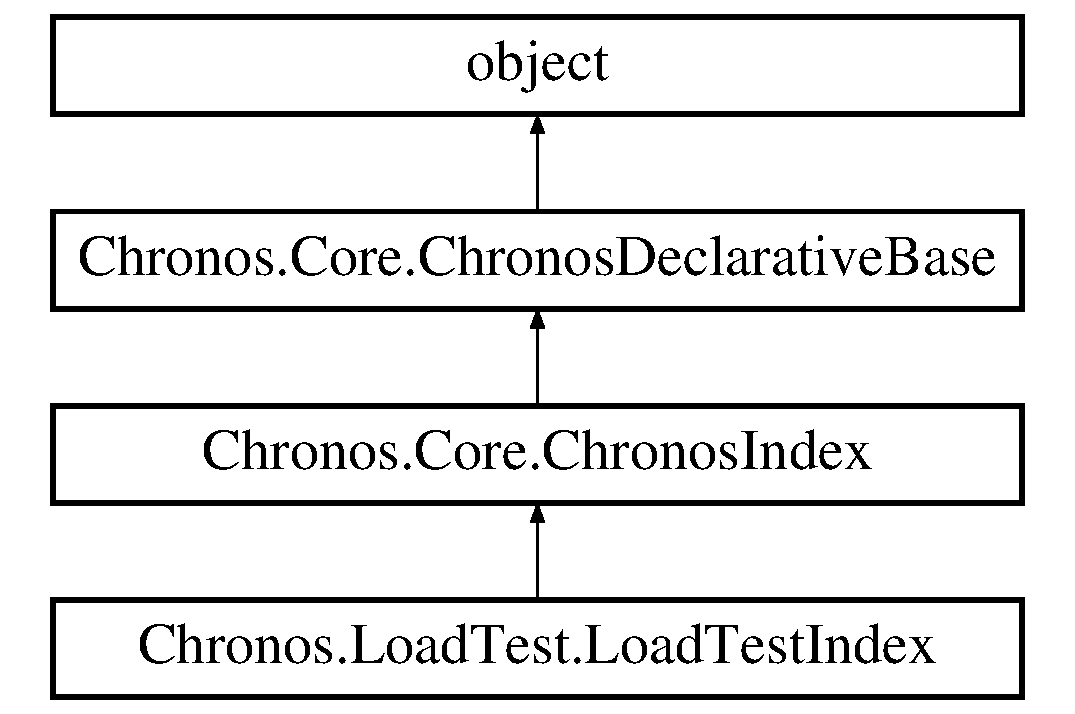
\includegraphics[height=4.000000cm]{classChronos_1_1Core_1_1ChronosDeclarativeBase}
\end{center}
\end{figure}
\subsection*{Public Member Functions}
\begin{DoxyCompactItemize}
\item 
def {\bfseries \+\_\+\+\_\+table\+\_\+args\+\_\+\+\_\+} (cls)
\item 
def {\bfseries To\+Json} (self)
\end{DoxyCompactItemize}
\subsection*{Static Public Attributes}
\begin{DoxyCompactItemize}
\item 
dictionary {\bfseries Base\+Config} = \{\textquotesingle{}extend\+\_\+existing\textquotesingle{}\+: True\}
\item 
list {\bfseries constraints} = \mbox{[}$\,$\mbox{]}
\end{DoxyCompactItemize}


The documentation for this class was generated from the following file\+:\begin{DoxyCompactItemize}
\item 
Chronos/Core.\+py\end{DoxyCompactItemize}

\hypertarget{classChronos_1_1Core_1_1ChronosDeclarativeMeta}{}\section{Chronos.\+Core.\+Chronos\+Declarative\+Meta Class Reference}
\label{classChronos_1_1Core_1_1ChronosDeclarativeMeta}\index{Chronos.\+Core.\+Chronos\+Declarative\+Meta@{Chronos.\+Core.\+Chronos\+Declarative\+Meta}}


A metaclass that tracks the current state of a Chronos declarative index.  


Inheritance diagram for Chronos.\+Core.\+Chronos\+Declarative\+Meta\+:\begin{figure}[H]
\begin{center}
\leavevmode
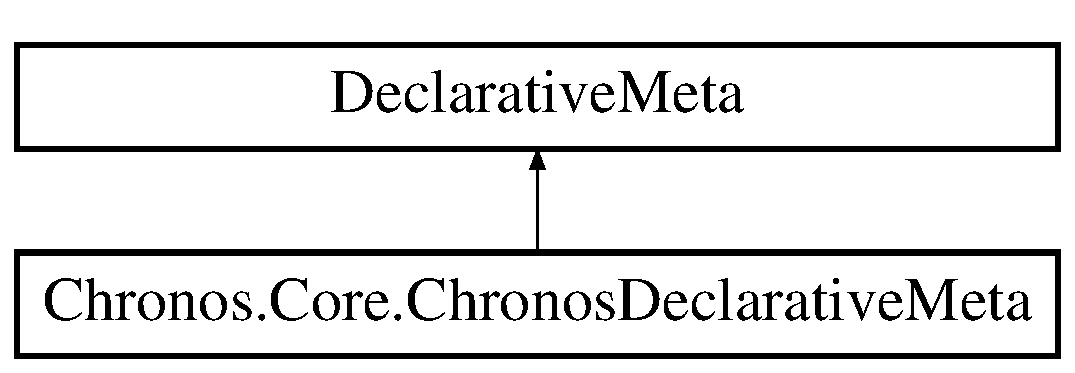
\includegraphics[height=2.000000cm]{classChronos_1_1Core_1_1ChronosDeclarativeMeta}
\end{center}
\end{figure}
\subsection*{Public Member Functions}
\begin{DoxyCompactItemize}
\item 
def {\bfseries \+\_\+\+\_\+init\+\_\+\+\_\+} (cls, classname, bases, dct)
\end{DoxyCompactItemize}
\subsection*{Public Attributes}
\begin{DoxyCompactItemize}
\item 
{\bfseries Indexed\+Attributes}
\end{DoxyCompactItemize}


\subsection{Detailed Description}
A metaclass that tracks the current state of a Chronos declarative index. 

This is required because S\+Q\+L\+Alchemy doesn\textquotesingle{}t have a built in way to remove columns that have already been attached to a table. Instead, we must manually ignore the \textquotesingle{}extra\textquotesingle{} columns through {\bfseries mapper\+\_\+args}. 

The documentation for this class was generated from the following file\+:\begin{DoxyCompactItemize}
\item 
Chronos/Core.\+py\end{DoxyCompactItemize}

\hypertarget{classChronos_1_1Core_1_1ChronosIndex}{}\section{Chronos.\+Core.\+Chronos\+Index Class Reference}
\label{classChronos_1_1Core_1_1ChronosIndex}\index{Chronos.\+Core.\+Chronos\+Index@{Chronos.\+Core.\+Chronos\+Index}}


The declarative base class for Chronos indices.  


Inheritance diagram for Chronos.\+Core.\+Chronos\+Index\+:\begin{figure}[H]
\begin{center}
\leavevmode
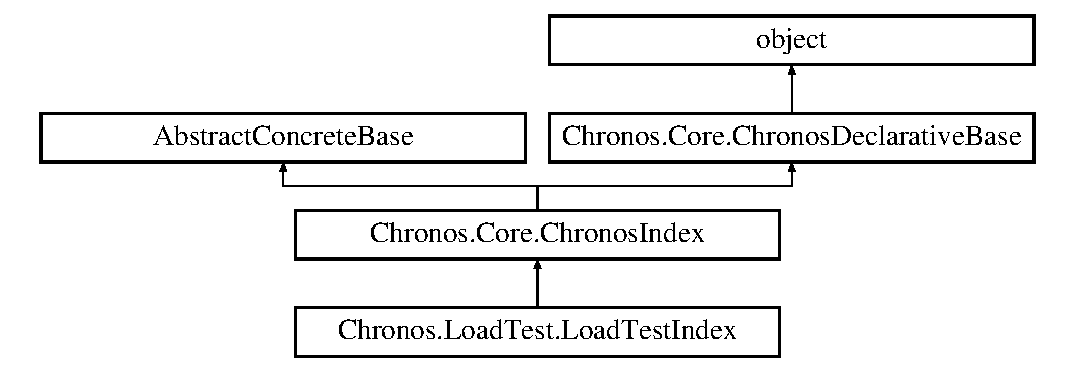
\includegraphics[height=4.000000cm]{classChronos_1_1Core_1_1ChronosIndex}
\end{center}
\end{figure}
\subsection*{Public Member Functions}
\begin{DoxyCompactItemize}
\item 
def {\bfseries \+\_\+\+\_\+tablename\+\_\+\+\_\+} (cls)
\item 
def {\bfseries \+\_\+\+\_\+mapper\+\_\+args\+\_\+\+\_\+} (cls)
\item 
def {\bfseries Create\+Tag\+Model} (cls)
\item 
def {\bfseries Create\+Checkpoint\+Model} (cls)
\end{DoxyCompactItemize}
\subsection*{Static Public Attributes}
\begin{DoxyCompactItemize}
\item 
tuple {\bfseries Shared\+Properties} = (\textquotesingle{}aggregate\+Id\textquotesingle{}, \textquotesingle{}is\+Archived\textquotesingle{}, \textquotesingle{}max\+Archived\+Version\textquotesingle{})
\item 
{\bfseries aggregate\+Id} = Column(Big\+Integer, primary\+\_\+key=True, autoincrement=False, nullable=False)
\item 
{\bfseries is\+Archived} = Column(Boolean, nullable=False, default=False)
\item 
{\bfseries max\+Archived\+Version} = Column(Big\+Integer, nullable=False, default=0)
\end{DoxyCompactItemize}


\subsection{Detailed Description}
The declarative base class for Chronos indices. 

This class expects subclasses to declare any aggregate properties that should be indexed as S\+Q\+L\+Alchemy Columns. Any constraints or sql indices should be provided via the constraints classmember.

It is important that the class name of a Chronos index class never changes -\/ this would cause a discrepancy in index table names through time and could result in permanent data loss. 

The documentation for this class was generated from the following file\+:\begin{DoxyCompactItemize}
\item 
Chronos/Core.\+py\end{DoxyCompactItemize}

\hypertarget{classChronos_1_1Core_1_1ChronosMeta}{}\section{Chronos.\+Core.\+Chronos\+Meta Class Reference}
\label{classChronos_1_1Core_1_1ChronosMeta}\index{Chronos.\+Core.\+Chronos\+Meta@{Chronos.\+Core.\+Chronos\+Meta}}


Provides common functionality for Chronos meta classes, \hyperlink{classChronos_1_1Core_1_1AggregateMeta}{Aggregate\+Meta} and \hyperlink{classChronos_1_1Core_1_1EventMeta}{Event\+Meta}.  


Inheritance diagram for Chronos.\+Core.\+Chronos\+Meta\+:\begin{figure}[H]
\begin{center}
\leavevmode
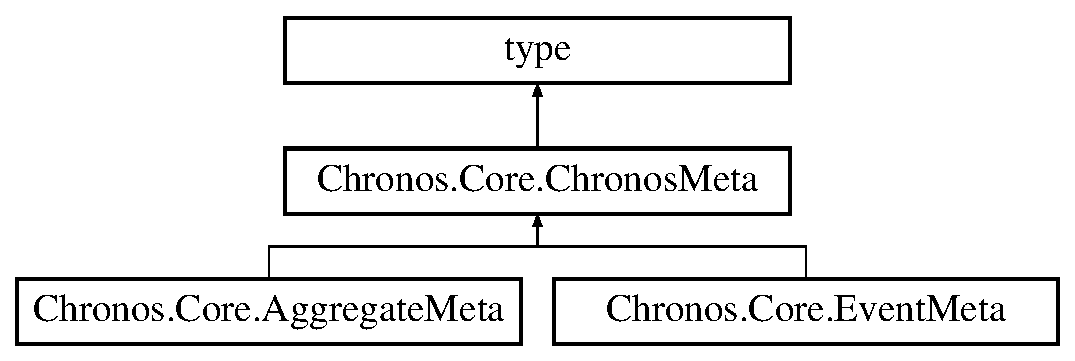
\includegraphics[height=3.000000cm]{classChronos_1_1Core_1_1ChronosMeta}
\end{center}
\end{figure}
\subsection*{Public Member Functions}
\begin{DoxyCompactItemize}
\item 
def {\bfseries \+\_\+\+\_\+init\+\_\+\+\_\+} (cls, name, bases, dct)
\end{DoxyCompactItemize}
\subsection*{Public Attributes}
\begin{DoxyCompactItemize}
\item 
{\bfseries full\+Name}
\end{DoxyCompactItemize}


\subsection{Detailed Description}
Provides common functionality for Chronos meta classes, \hyperlink{classChronos_1_1Core_1_1AggregateMeta}{Aggregate\+Meta} and \hyperlink{classChronos_1_1Core_1_1EventMeta}{Event\+Meta}. 

\hyperlink{classChronos_1_1Core_1_1ChronosMeta}{Chronos\+Meta} ensures that classes have a \textquotesingle{}Proto\textquotesingle{} attribute, and that the attribute is a protobuf class. As a convenience, \hyperlink{classChronos_1_1Core_1_1ChronosMeta}{Chronos\+Meta} also adds a \textquotesingle{}full\+Name\textquotesingle{} class member for use elsewhere in Chronos\+::\+Core. 

The documentation for this class was generated from the following file\+:\begin{DoxyCompactItemize}
\item 
Chronos/Core.\+py\end{DoxyCompactItemize}

\hypertarget{classChronos_1_1Core_1_1ChronosSemanticException}{}\section{Chronos.\+Core.\+Chronos\+Semantic\+Exception Class Reference}
\label{classChronos_1_1Core_1_1ChronosSemanticException}\index{Chronos.\+Core.\+Chronos\+Semantic\+Exception@{Chronos.\+Core.\+Chronos\+Semantic\+Exception}}


An Exception indicating that Chronos has encountered a class that violates required semantics for event sourcing or notification.  


Inheritance diagram for Chronos.\+Core.\+Chronos\+Semantic\+Exception\+:\begin{figure}[H]
\begin{center}
\leavevmode
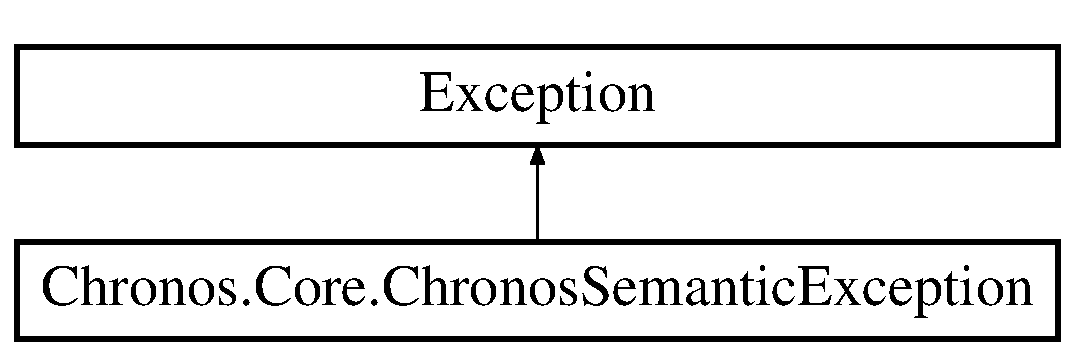
\includegraphics[height=2.000000cm]{classChronos_1_1Core_1_1ChronosSemanticException}
\end{center}
\end{figure}


\subsection{Detailed Description}
An Exception indicating that Chronos has encountered a class that violates required semantics for event sourcing or notification. 



The documentation for this class was generated from the following file\+:\begin{DoxyCompactItemize}
\item 
Chronos/Core.\+py\end{DoxyCompactItemize}

\hypertarget{classChronos_1_1Core_1_1Event}{}\section{Chronos.\+Core.\+Event Class Reference}
\label{classChronos_1_1Core_1_1Event}\index{Chronos.\+Core.\+Event@{Chronos.\+Core.\+Event}}


The public \hyperlink{classChronos_1_1Core_1_1Event}{Event} base class.  


Inheritance diagram for Chronos.\+Core.\+Event\+:\begin{figure}[H]
\begin{center}
\leavevmode
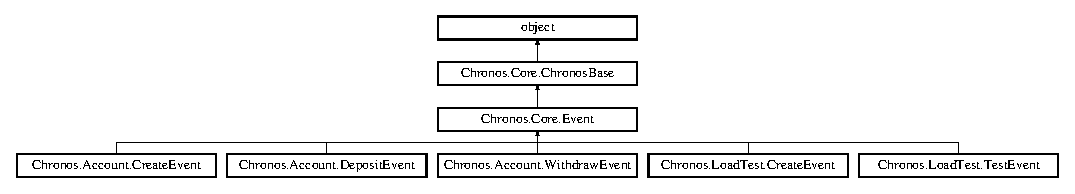
\includegraphics[height=2.164251cm]{classChronos_1_1Core_1_1Event}
\end{center}
\end{figure}
\subsection*{Public Member Functions}
\begin{DoxyCompactItemize}
\item 
def {\bfseries \+\_\+\+\_\+init\+\_\+\+\_\+} (self, version, logic\+Version)
\item 
def {\bfseries To\+Proto} (self, received\+Timestamp, processed\+Timestamp)
\end{DoxyCompactItemize}
\subsection*{Static Public Member Functions}
\begin{DoxyCompactItemize}
\item 
def {\bfseries From\+Proto\+String} (string)
\end{DoxyCompactItemize}
\subsection*{Public Attributes}
\begin{DoxyCompactItemize}
\item 
{\bfseries version}
\item 
{\bfseries logic\+Version}
\end{DoxyCompactItemize}


\subsection{Detailed Description}
The public \hyperlink{classChronos_1_1Core_1_1Event}{Event} base class. 

This mainly exists to connect \hyperlink{classChronos_1_1Core_1_1EventMeta}{Event\+Meta} and \hyperlink{classChronos_1_1Core_1_1ChronosBase}{Chronos\+Base} so that the client can subclass a single class in their code. 

The documentation for this class was generated from the following file\+:\begin{DoxyCompactItemize}
\item 
Chronos/Core.\+py\end{DoxyCompactItemize}

\hypertarget{classChronos_1_1Core_1_1EventMeta}{}\section{Chronos.\+Core.\+Event\+Meta Class Reference}
\label{classChronos_1_1Core_1_1EventMeta}\index{Chronos.\+Core.\+Event\+Meta@{Chronos.\+Core.\+Event\+Meta}}


Validates and sets up classes as proper Chronos Events.  


Inheritance diagram for Chronos.\+Core.\+Event\+Meta\+:\begin{figure}[H]
\begin{center}
\leavevmode
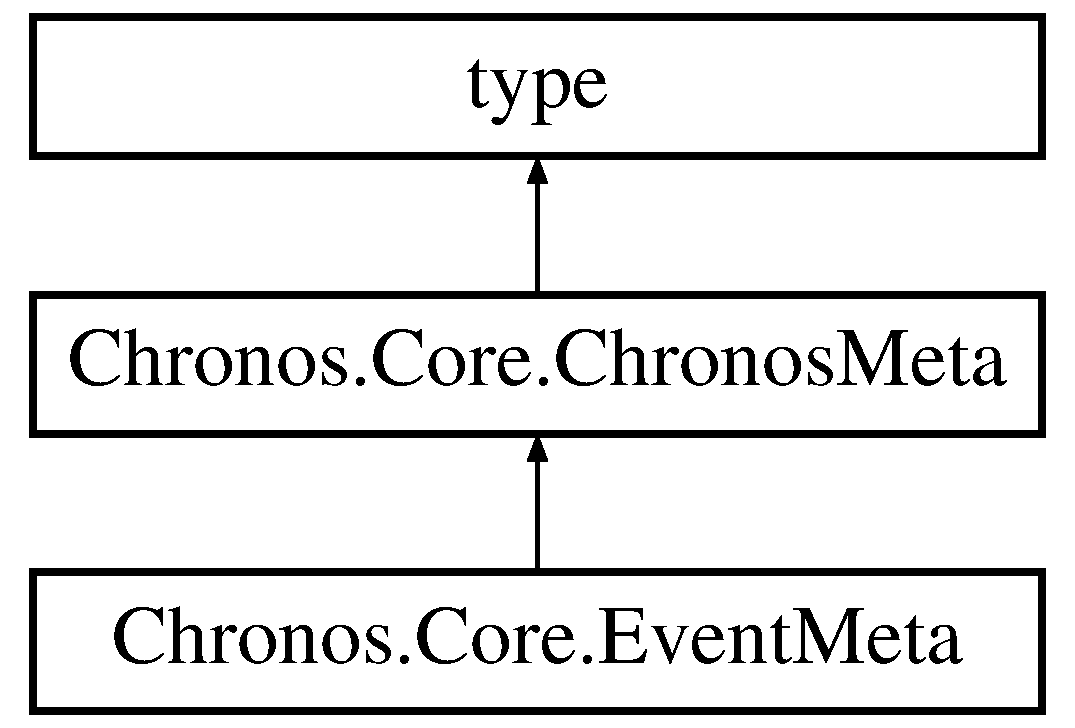
\includegraphics[height=3.000000cm]{classChronos_1_1Core_1_1EventMeta}
\end{center}
\end{figure}
\subsection*{Public Member Functions}
\begin{DoxyCompactItemize}
\item 
def {\bfseries \+\_\+\+\_\+init\+\_\+\+\_\+} (cls, name, bases, dct)
\end{DoxyCompactItemize}
\subsection*{Public Attributes}
\begin{DoxyCompactItemize}
\item 
{\bfseries Dependencies}
\item 
{\bfseries Raise\+For}
\end{DoxyCompactItemize}


\subsection{Detailed Description}
Validates and sets up classes as proper Chronos Events. 

Defining an \hyperlink{classChronos_1_1Core_1_1EventMeta}{Event\+Meta} will enforce that the \hyperlink{classChronos_1_1Core_1_1Event}{Event} specifies a proper \hyperlink{classChronos_1_1Core_1_1Aggregate}{Aggregate} and that the \hyperlink{classChronos_1_1Core_1_1Event}{Event} implements required functionality for Chronos processing. 

The documentation for this class was generated from the following file\+:\begin{DoxyCompactItemize}
\item 
Chronos/Core.\+py\end{DoxyCompactItemize}

\hypertarget{classChronos_1_1Core_1_1EventProcessor}{}\section{Chronos.\+Core.\+Event\+Processor Class Reference}
\label{classChronos_1_1Core_1_1EventProcessor}\index{Chronos.\+Core.\+Event\+Processor@{Chronos.\+Core.\+Event\+Processor}}


Handles processing and replay of events against aggregate instances.  


Inheritance diagram for Chronos.\+Core.\+Event\+Processor\+:\begin{figure}[H]
\begin{center}
\leavevmode
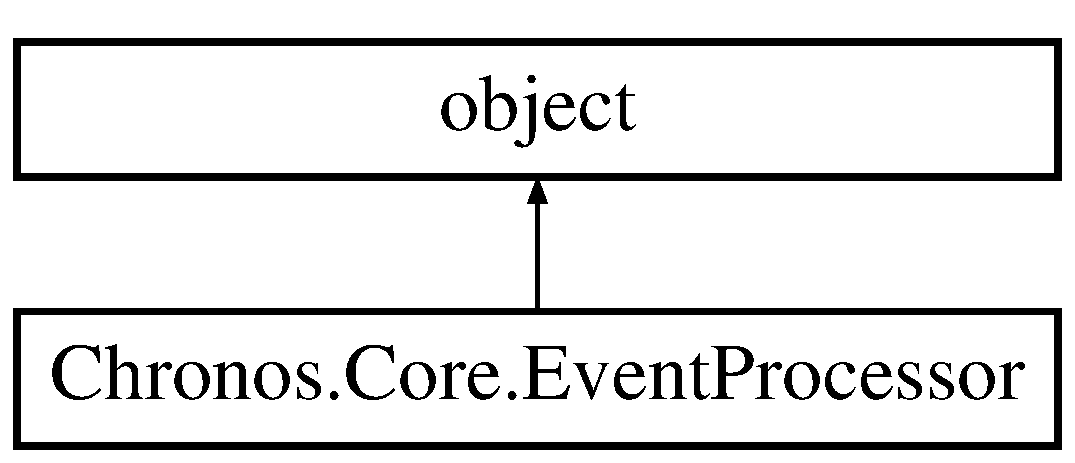
\includegraphics[height=2.000000cm]{classChronos_1_1Core_1_1EventProcessor}
\end{center}
\end{figure}
\subsection*{Public Member Functions}
\begin{DoxyCompactItemize}
\item 
def {\bfseries \+\_\+\+\_\+init\+\_\+\+\_\+} (self, event\+Store, logic\+Compiler, persistence\+Pool=None)
\item 
def {\bfseries Begin} (self)
\item 
def {\bfseries Commit} (self)
\item 
def {\bfseries Rollback} (self)
\item 
def \hyperlink{group__Chronos_gaa715d77da2ab4a07c97ddc27b6691b69}{Process} (self, request, aggregate, single\+Event)
\begin{DoxyCompactList}\small\item\em Applies the provided event to the provided aggregate. \end{DoxyCompactList}\item 
def \hyperlink{group__Chronos_gaef2d2639259438495b17f1ab5903bbb7}{Process\+Index\+Divergence} (self, aggregate\+Class, aggregate\+Id)
\begin{DoxyCompactList}\small\item\em Notifies clients that an aggregate instance has diverged indices. \end{DoxyCompactList}\item 
def \hyperlink{group__Chronos_ga9ec5fe085282e9ee1909ee9b5752e44b}{Process\+Failure} (self, request, aggregate\+Class, exception)
\begin{DoxyCompactList}\small\item\em Notifies clients that an event processing request has failed. \end{DoxyCompactList}\item 
def {\bfseries Process\+Tag} (self, aggregate, tag, tag\+Expiration, create\+Date=long(time.\+time()))
\item 
def {\bfseries Enqueue\+For\+Persistence} (self, buffer\+Item)
\item 
def {\bfseries Flush\+Persistence\+Buffer} (self, aggregate\+Class, should\+Force=False)
\item 
def \hyperlink{group__Chronos_gab6aa538a4b382256b1b168a274adab7f}{Replay\+By\+Timestamp\+Range} (self, aggregate, from\+Timestamp, to\+Timestamp)
\begin{DoxyCompactList}\small\item\em Applies all events processed later than the from\+Timestamp and before the to\+Timestamp of the supplied aggregate to the same instance. \end{DoxyCompactList}\item 
def \hyperlink{group__Chronos_gae2b807dba975704f1e383eef0df911c6}{Replay\+To\+Version} (self, aggregate, to\+Version)
\begin{DoxyCompactList}\small\item\em Applies all events later than the current version of the supplied aggregate to that same instance. \end{DoxyCompactList}\end{DoxyCompactItemize}
\subsection*{Public Attributes}
\begin{DoxyCompactItemize}
\item 
{\bfseries event\+Store}
\item 
{\bfseries logic\+Compiler}
\item 
{\bfseries persistence\+Buffer}
\item 
{\bfseries persistence\+Pool}
\item 
{\bfseries lock}
\item 
{\bfseries is\+Replaying}
\item 
{\bfseries transaction\+Buffer}
\end{DoxyCompactItemize}
\subsection*{Static Public Attributes}
\begin{DoxyCompactItemize}
\item 
int {\bfseries Max\+Buffered\+Events} = 15
\end{DoxyCompactItemize}


\subsection{Detailed Description}
Handles processing and replay of events against aggregate instances. 

This class is thread-\/safe. 

The documentation for this class was generated from the following file\+:\begin{DoxyCompactItemize}
\item 
Chronos/Core.\+py\end{DoxyCompactItemize}

\hypertarget{classChronos_1_1Core_1_1IndexStore}{}\section{Chronos.\+Core.\+Index\+Store Class Reference}
\label{classChronos_1_1Core_1_1IndexStore}\index{Chronos.\+Core.\+Index\+Store@{Chronos.\+Core.\+Index\+Store}}


Handles all interaction relating to Chronos indexing functionality.  


Inheritance diagram for Chronos.\+Core.\+Index\+Store\+:\begin{figure}[H]
\begin{center}
\leavevmode
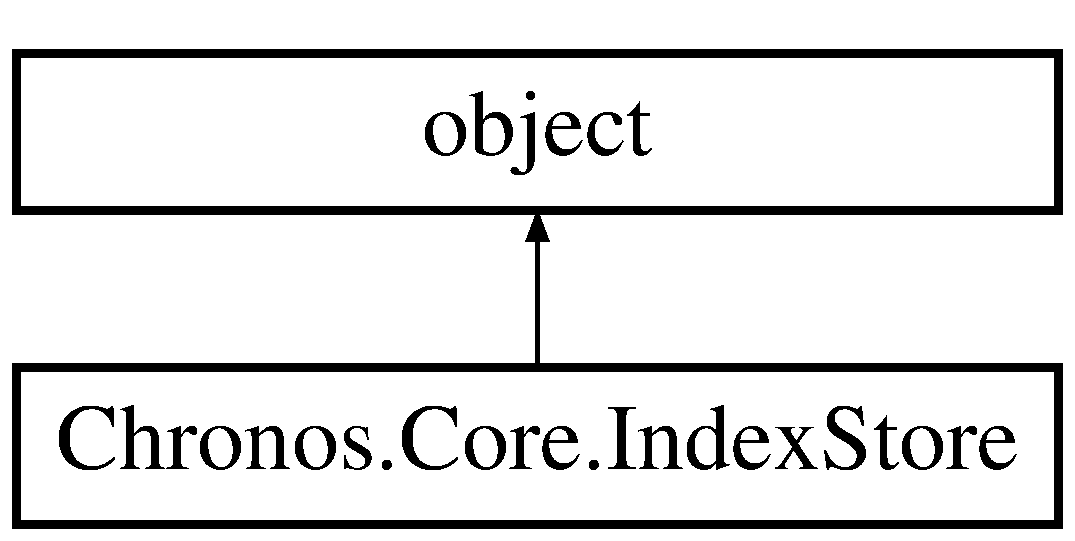
\includegraphics[height=2.000000cm]{classChronos_1_1Core_1_1IndexStore}
\end{center}
\end{figure}
\subsection*{Public Member Functions}
\begin{DoxyCompactItemize}
\item 
def {\bfseries \+\_\+\+\_\+init\+\_\+\+\_\+} (self, aggregate\+Class)
\item 
def {\bfseries Dispose} (self)
\item 
def {\bfseries Get\+Session} (self)
\item 
def \hyperlink{group__Chronos_gac76ddb048aa12434e964963fe6b08abc}{Get\+Checkpoint} (self, session)
\begin{DoxyCompactList}\small\item\em Retrieves the current checkpoint information from the S\+Q\+Lite instance. \end{DoxyCompactList}\item 
def \hyperlink{group__Chronos_ga999de3bf409634d23dbdce8483f38beb}{Update\+Checkpoint} (self, max\+Request\+Id, session)
\begin{DoxyCompactList}\small\item\em Persists the provided max\+Request\+Id into the S\+Q\+Lite instance\textquotesingle{}s checkpoint. \end{DoxyCompactList}\item 
def \hyperlink{group__Chronos_gadee7d443d8b7f4f600db3e666388bfd2}{Reindex\+Aggregate} (self, aggregate, session)
\begin{DoxyCompactList}\small\item\em Upserts the provided aggregate\textquotesingle{}s information into the underlying sqlite database. \end{DoxyCompactList}\item 
def \hyperlink{group__Chronos_ga3f3b13bc9ea88c0ff50c1da74c76baa3}{Index\+Tag} (self, tag, aggregate\+Id, session)
\begin{DoxyCompactList}\small\item\em Persists the provided tag information to the S\+Q\+Lite instance. \end{DoxyCompactList}\item 
def {\bfseries Get\+Index\+Row} (self, aggregate\+Id)
\item 
def {\bfseries Get\+Tag\+Row} (self, aggregate\+Id, tag)
\item 
def {\bfseries Get\+Tags\+By\+Aggregate\+Id} (self, aggregate\+Id)
\item 
def {\bfseries Get\+All\+Tags} (self)
\item 
def \hyperlink{group__Chronos_gae214bee43e5148b5190c7ba0f6aa63ef}{Mark\+Tags\+As\+Archived} (self, tags)
\begin{DoxyCompactList}\small\item\em Updates the provided tags to mark them as archived (no longer available via Redis). \end{DoxyCompactList}\item 
def \hyperlink{group__Chronos_ga04d2c0aa20ac6cfe356b724e8c62dd8b}{Mark\+As\+Archived} (self, aggregate\+Ids)
\begin{DoxyCompactList}\small\item\em Updates the provided aggregate to mark it as archived. \end{DoxyCompactList}\item 
def \hyperlink{group__Chronos_gae824d1e632ce32a311c6a07756f17c28}{Update\+Max\+Archived\+Version} (self, aggregate\+Id, max\+Version)
\begin{DoxyCompactList}\small\item\em Updates the provided aggregate with its maximum archived version. \end{DoxyCompactList}\item 
def \hyperlink{group__Chronos_ga960e19d8f65569f80fd580eebd605031}{Retrieve\+Aggregate\+Ids} (self, is\+Archived=False, indices)
\begin{DoxyCompactList}\small\item\em Returns a list of all aggregate\+Ids that satisfy the provided index properties. \end{DoxyCompactList}\item 
def \hyperlink{group__Chronos_ga3e51459a6d624a6abf12d983139e6acd}{Retrieve\+Aggregates} (self, from\+Aggregate\+Id, return\+Count, is\+Archived=False, indices)
\begin{DoxyCompactList}\small\item\em Returns a list of all aggregates and their index properties that satisfy the provided index properties. \end{DoxyCompactList}\end{DoxyCompactItemize}
\subsection*{Static Public Member Functions}
\begin{DoxyCompactItemize}
\item 
def \hyperlink{group__Chronos_ga03ff3b6b6e521bc886259e7b8f390819}{Update\+Index\+Schema} (aggregate\+Class)
\begin{DoxyCompactList}\small\item\em Executes an external procedure that updates the underlying sqlite database using an on-\/disk alembic configuration. \end{DoxyCompactList}\item 
def {\bfseries Get\+Index\+Store} (aggregate\+Name, event\+Store, logic\+Compiler)
\end{DoxyCompactItemize}
\subsection*{Public Attributes}
\begin{DoxyCompactItemize}
\item 
{\bfseries aggregate\+Class}
\item 
{\bfseries index\+Class}
\item 
{\bfseries tag\+Class}
\item 
{\bfseries checkpoint\+Class}
\item 
{\bfseries sqlite\+Path}
\item 
{\bfseries engine}
\item 
{\bfseries read\+Engine}
\item 
{\bfseries session\+Maker}
\item 
{\bfseries read\+Session\+Maker}
\end{DoxyCompactItemize}
\subsection*{Static Public Attributes}
\begin{DoxyCompactItemize}
\item 
{\bfseries Schema\+Lock} = Lock()
\item 
string {\bfseries S\+Q\+Lite\+Path\+Template} = \textquotesingle{}sqlite\+:////var/lib/chronos/index.\+alembic/db/\{0\}.sqlite\textquotesingle{}
\end{DoxyCompactItemize}


\subsection{Detailed Description}
Handles all interaction relating to Chronos indexing functionality. 

The \hyperlink{classChronos_1_1Core_1_1IndexStore}{Index\+Store} interfaces with sqlite databases instances that are persisted on disk as part of the Chronos running configuration. In production, these databases (and the entire Chronos running configuration) are persisted on network storage (the Nimble device, currently) in case of individual server failure.

Instances of this class are not thread-\/safe. 

The documentation for this class was generated from the following file\+:\begin{DoxyCompactItemize}
\item 
Chronos/Core.\+py\end{DoxyCompactItemize}

\hypertarget{classChronos_1_1Core_1_1NoEventsFound}{}\section{Chronos.\+Core.\+No\+Events\+Found Class Reference}
\label{classChronos_1_1Core_1_1NoEventsFound}\index{Chronos.\+Core.\+No\+Events\+Found@{Chronos.\+Core.\+No\+Events\+Found}}
Inheritance diagram for Chronos.\+Core.\+No\+Events\+Found\+:\begin{figure}[H]
\begin{center}
\leavevmode
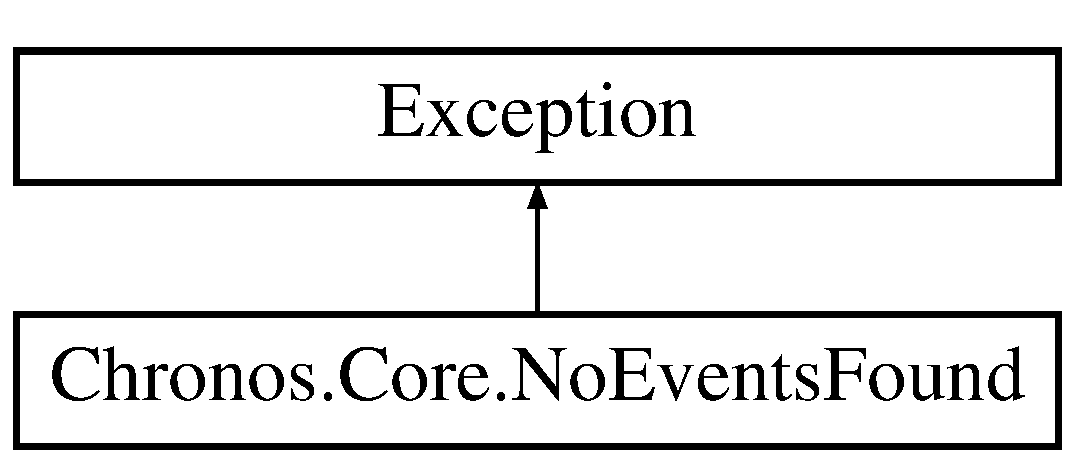
\includegraphics[height=2.000000cm]{classChronos_1_1Core_1_1NoEventsFound}
\end{center}
\end{figure}


The documentation for this class was generated from the following file\+:\begin{DoxyCompactItemize}
\item 
Chronos/Core.\+py\end{DoxyCompactItemize}

\hypertarget{classChronos_1_1Core_1_1SqliteIndex}{}\section{Chronos.\+Core.\+Sqlite\+Index Class Reference}
\label{classChronos_1_1Core_1_1SqliteIndex}\index{Chronos.\+Core.\+Sqlite\+Index@{Chronos.\+Core.\+Sqlite\+Index}}


Abstracts away the details of the sqlite index implementation.  


Inheritance diagram for Chronos.\+Core.\+Sqlite\+Index\+:\begin{figure}[H]
\begin{center}
\leavevmode
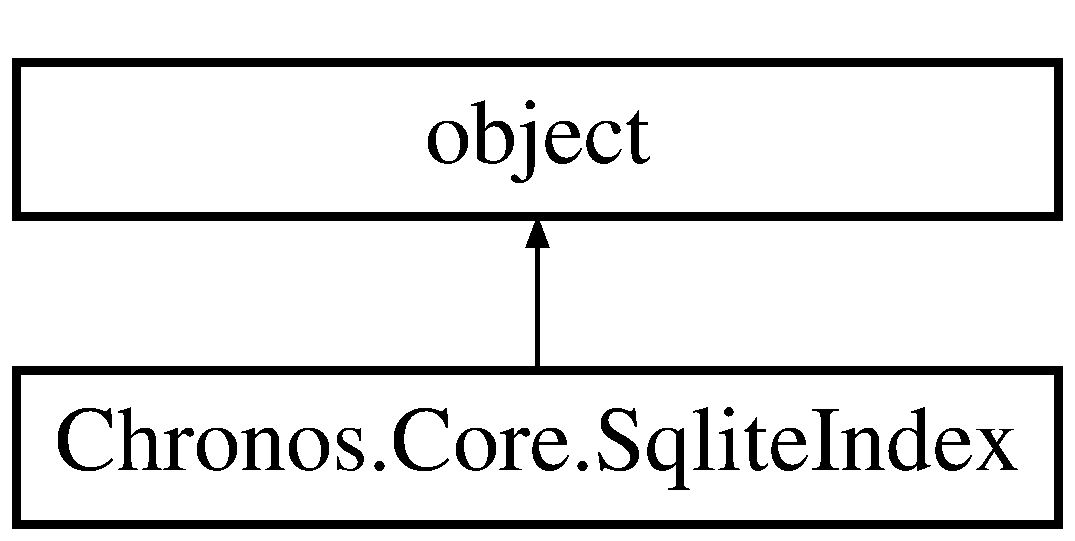
\includegraphics[height=2.000000cm]{classChronos_1_1Core_1_1SqliteIndex}
\end{center}
\end{figure}
\subsection*{Public Member Functions}
\begin{DoxyCompactItemize}
\item 
def {\bfseries \+\_\+\+\_\+init\+\_\+\+\_\+} (self, sqlite\+Session)
\item 
def {\bfseries Begin} (self)
\item 
def {\bfseries Commit} (self)
\item 
def {\bfseries Rollback} (self)
\item 
def {\bfseries Close} (self)
\item 
def {\bfseries Add} (self, obj)
\item 
def {\bfseries Flush} (self)
\end{DoxyCompactItemize}
\subsection*{Public Attributes}
\begin{DoxyCompactItemize}
\item 
{\bfseries sqlite\+Session}
\end{DoxyCompactItemize}


\subsection{Detailed Description}
Abstracts away the details of the sqlite index implementation. 

This class mainly exists to provide the same transactional interface provided by \hyperlink{classChronos_1_1Core_1_1AggregateRepository}{Aggregate\+Repository} and \hyperlink{classChronos_1_1Core_1_1EventProcessor}{Event\+Processor}. 

The documentation for this class was generated from the following file\+:\begin{DoxyCompactItemize}
\item 
Chronos/Core.\+py\end{DoxyCompactItemize}

\hypertarget{classChronos_1_1Core_1_1ValidationError}{}\section{Chronos.\+Core.\+Validation\+Error Class Reference}
\label{classChronos_1_1Core_1_1ValidationError}\index{Chronos.\+Core.\+Validation\+Error@{Chronos.\+Core.\+Validation\+Error}}


An Exception for use in \hyperlink{classChronos_1_1Core_1_1Event}{Event} subclasses to indicate that the event is logically invalid.  


Inheritance diagram for Chronos.\+Core.\+Validation\+Error\+:\begin{figure}[H]
\begin{center}
\leavevmode
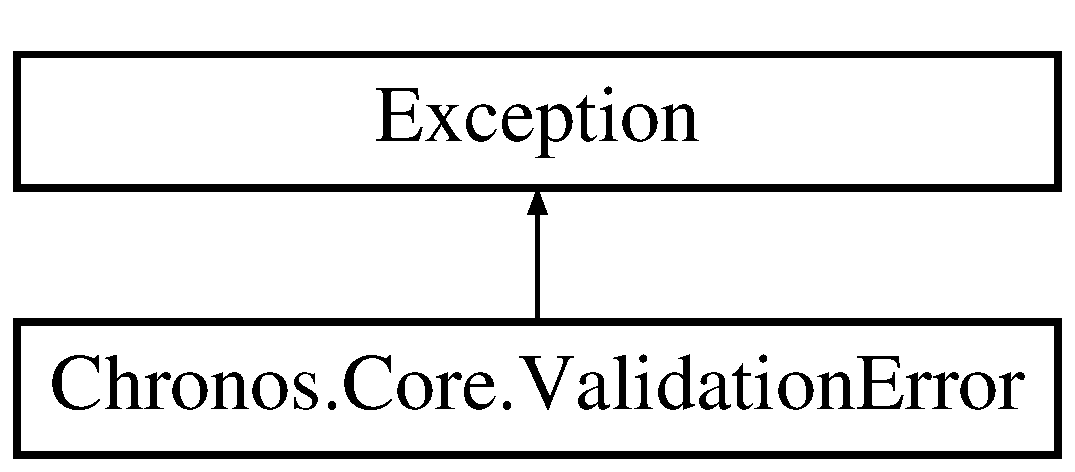
\includegraphics[height=2.000000cm]{classChronos_1_1Core_1_1ValidationError}
\end{center}
\end{figure}
\subsection*{Public Member Functions}
\begin{DoxyCompactItemize}
\item 
def {\bfseries \+\_\+\+\_\+init\+\_\+\+\_\+} (self, exception\+Message, tags=None)
\end{DoxyCompactItemize}
\subsection*{Public Attributes}
\begin{DoxyCompactItemize}
\item 
{\bfseries tags}
\end{DoxyCompactItemize}


\subsection{Detailed Description}
An Exception for use in \hyperlink{classChronos_1_1Core_1_1Event}{Event} subclasses to indicate that the event is logically invalid. 

Raising this Exception from within Event\+::\+Raise\+For will still cause the event application to fail, but the failure will not be logged as an error. 

The documentation for this class was generated from the following file\+:\begin{DoxyCompactItemize}
\item 
Chronos/Core.\+py\end{DoxyCompactItemize}

\hypertarget{classChronos_1_1DefaultImplementations_1_1GetLatestAggregateLogic}{}\section{Chronos.\+Default\+Implementations.\+Get\+Latest\+Aggregate\+Logic Class Reference}
\label{classChronos_1_1DefaultImplementations_1_1GetLatestAggregateLogic}\index{Chronos.\+Default\+Implementations.\+Get\+Latest\+Aggregate\+Logic@{Chronos.\+Default\+Implementations.\+Get\+Latest\+Aggregate\+Logic}}


A Lua script for retrieval of the latest Aggregate\+Logic for a given Aggregate.  


Inheritance diagram for Chronos.\+Default\+Implementations.\+Get\+Latest\+Aggregate\+Logic\+:\begin{figure}[H]
\begin{center}
\leavevmode
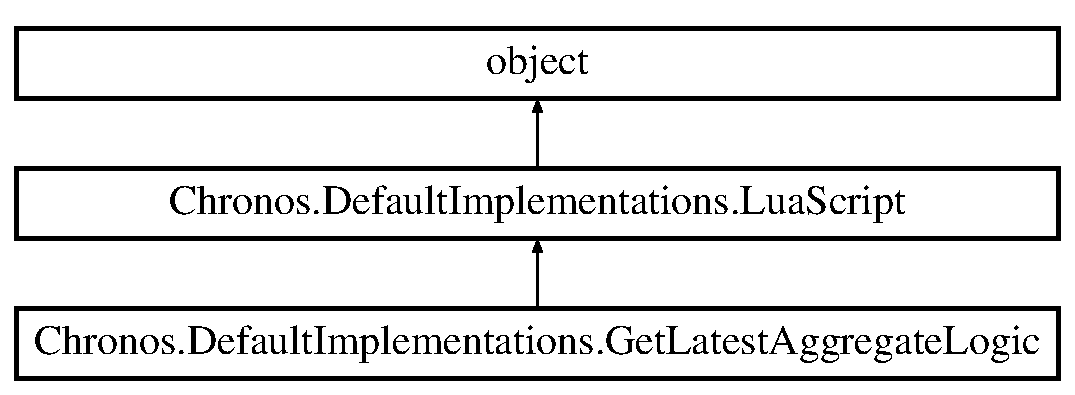
\includegraphics[height=3.000000cm]{classChronos_1_1DefaultImplementations_1_1GetLatestAggregateLogic}
\end{center}
\end{figure}
\subsection*{Public Member Functions}
\begin{DoxyCompactItemize}
\item 
def {\bfseries \+\_\+\+\_\+init\+\_\+\+\_\+} (self, logic\+Id\+Key, logic\+Key)
\item 
def {\bfseries Parse\+Redis\+Result} (self, redis\+Result)
\end{DoxyCompactItemize}
\subsection*{Static Public Attributes}
\begin{DoxyCompactItemize}
\item 
string {\bfseries Logic\+Lua\+Script}
\end{DoxyCompactItemize}
\subsection*{Additional Inherited Members}


\subsection{Detailed Description}
A Lua script for retrieval of the latest Aggregate\+Logic for a given Aggregate. 

The documentation for this class was generated from the following file\+:\begin{DoxyCompactItemize}
\item 
Chronos/Default\+Implementations.\+py\end{DoxyCompactItemize}

\hypertarget{classChronos_1_1DefaultImplementations_1_1GetSnapshotsFromIndex}{}\section{Chronos.\+Default\+Implementations.\+Get\+Snapshots\+From\+Index Class Reference}
\label{classChronos_1_1DefaultImplementations_1_1GetSnapshotsFromIndex}\index{Chronos.\+Default\+Implementations.\+Get\+Snapshots\+From\+Index@{Chronos.\+Default\+Implementations.\+Get\+Snapshots\+From\+Index}}


A Lua script for transactional retrieval of snapshots from index pointers.  


Inheritance diagram for Chronos.\+Default\+Implementations.\+Get\+Snapshots\+From\+Index\+:\begin{figure}[H]
\begin{center}
\leavevmode
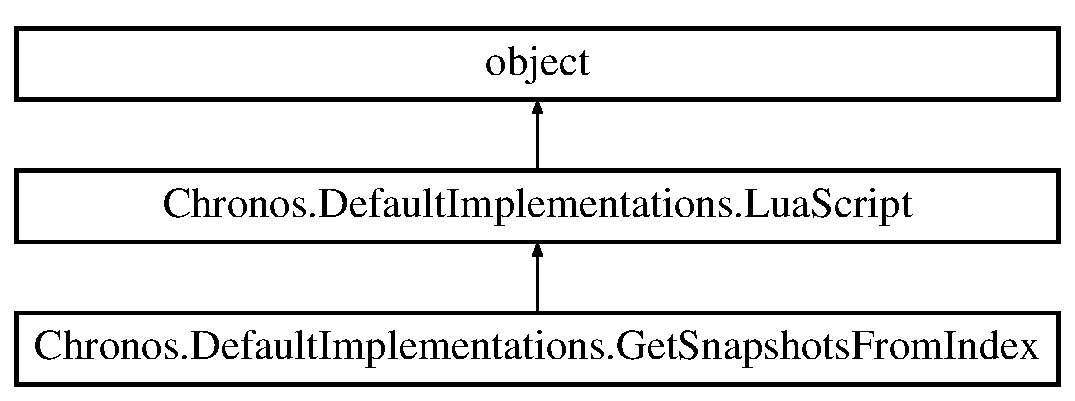
\includegraphics[height=3.000000cm]{classChronos_1_1DefaultImplementations_1_1GetSnapshotsFromIndex}
\end{center}
\end{figure}
\subsection*{Public Member Functions}
\begin{DoxyCompactItemize}
\item 
def {\bfseries \+\_\+\+\_\+init\+\_\+\+\_\+} (self, keys)
\item 
def {\bfseries Parse\+Redis\+Result} (self, redis\+Result)
\end{DoxyCompactItemize}
\subsection*{Static Public Attributes}
\begin{DoxyCompactItemize}
\item 
string {\bfseries Index\+Lua\+Script}
\end{DoxyCompactItemize}
\subsection*{Additional Inherited Members}


\subsection{Detailed Description}
A Lua script for transactional retrieval of snapshots from index pointers. 



The documentation for this class was generated from the following file\+:\begin{DoxyCompactItemize}
\item 
Chronos/Default\+Implementations.\+py\end{DoxyCompactItemize}

\hypertarget{classChronos_1_1DefaultImplementations_1_1LuaScript}{}\section{Chronos.\+Default\+Implementations.\+Lua\+Script Class Reference}
\label{classChronos_1_1DefaultImplementations_1_1LuaScript}\index{Chronos.\+Default\+Implementations.\+Lua\+Script@{Chronos.\+Default\+Implementations.\+Lua\+Script}}
Inheritance diagram for Chronos.\+Default\+Implementations.\+Lua\+Script\+:\begin{figure}[H]
\begin{center}
\leavevmode
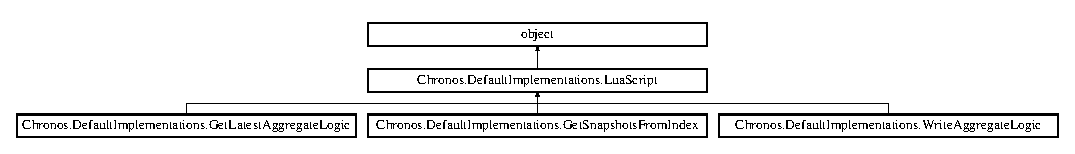
\includegraphics[height=1.618497cm]{classChronos_1_1DefaultImplementations_1_1LuaScript}
\end{center}
\end{figure}
\subsection*{Public Member Functions}
\begin{DoxyCompactItemize}
\item 
def {\bfseries \+\_\+\+\_\+init\+\_\+\+\_\+} (self, lua\+Script, keys=None, argv=None)
\item 
def {\bfseries Parse\+Redis\+Result} (self, redis\+Result)
\item 
def {\bfseries Eval} (self, redis\+Connection)
\end{DoxyCompactItemize}
\subsection*{Public Attributes}
\begin{DoxyCompactItemize}
\item 
{\bfseries lua\+Script}
\item 
{\bfseries keys}
\item 
{\bfseries argv}
\end{DoxyCompactItemize}


The documentation for this class was generated from the following file\+:\begin{DoxyCompactItemize}
\item 
Chronos/Default\+Implementations.\+py\end{DoxyCompactItemize}

\hypertarget{classChronos_1_1DefaultImplementations_1_1RedisEventKeys}{}\section{Chronos.\+Default\+Implementations.\+Redis\+Event\+Keys Class Reference}
\label{classChronos_1_1DefaultImplementations_1_1RedisEventKeys}\index{Chronos.\+Default\+Implementations.\+Redis\+Event\+Keys@{Chronos.\+Default\+Implementations.\+Redis\+Event\+Keys}}
Inheritance diagram for Chronos.\+Default\+Implementations.\+Redis\+Event\+Keys\+:\begin{figure}[H]
\begin{center}
\leavevmode
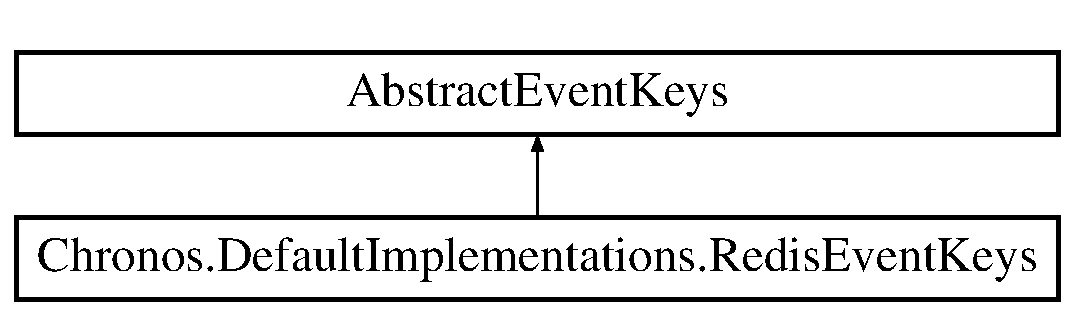
\includegraphics[height=2.000000cm]{classChronos_1_1DefaultImplementations_1_1RedisEventKeys}
\end{center}
\end{figure}
\subsection*{Public Member Functions}
\begin{DoxyCompactItemize}
\item 
def {\bfseries \+\_\+\+\_\+init\+\_\+\+\_\+} (self, aggregate\+Class)
\item 
def {\bfseries Get\+Event\+Key} (self, aggregate\+Id)
\item 
def {\bfseries Get\+Snapshot\+Key} (self, aggregate\+Id)
\item 
def {\bfseries Get\+Tag\+Wildcard} (self)
\item 
def {\bfseries Get\+Tag\+Key} (self, aggregate\+Id, tag)
\item 
def {\bfseries Get\+Publishing\+Topic} (self, aggregate)
\item 
def {\bfseries Get\+Failure\+Topic} (self)
\item 
def {\bfseries Get\+Management\+Topic} (self)
\end{DoxyCompactItemize}
\subsection*{Public Attributes}
\begin{DoxyCompactItemize}
\item 
{\bfseries aggregate\+Class}
\item 
{\bfseries hash\+Key}
\item 
{\bfseries id\+Key}
\item 
{\bfseries logic\+Id\+Key}
\item 
{\bfseries logic\+Key}
\item 
{\bfseries checkpoint\+Key}
\end{DoxyCompactItemize}


The documentation for this class was generated from the following file\+:\begin{DoxyCompactItemize}
\item 
Chronos/Default\+Implementations.\+py\end{DoxyCompactItemize}

\hypertarget{classChronos_1_1DefaultImplementations_1_1RedisEventStore}{}\section{Chronos.\+Default\+Implementations.\+Redis\+Event\+Store Class Reference}
\label{classChronos_1_1DefaultImplementations_1_1RedisEventStore}\index{Chronos.\+Default\+Implementations.\+Redis\+Event\+Store@{Chronos.\+Default\+Implementations.\+Redis\+Event\+Store}}


An event store implementation using Redis as the backend for both event persistence and notification.  


Inheritance diagram for Chronos.\+Default\+Implementations.\+Redis\+Event\+Store\+:\begin{figure}[H]
\begin{center}
\leavevmode
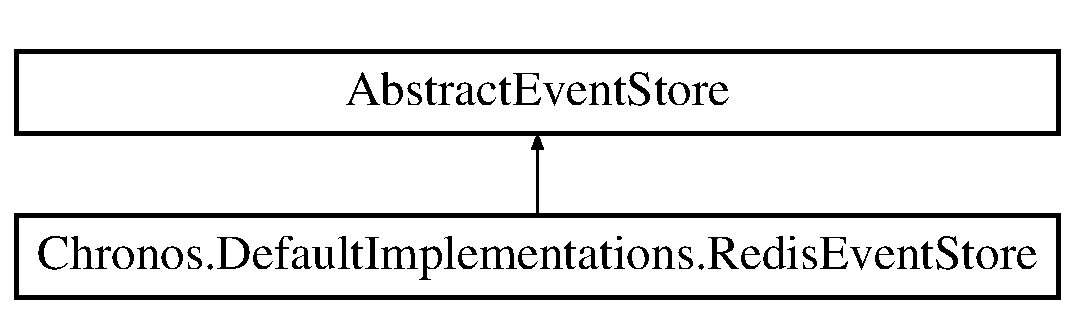
\includegraphics[height=2.000000cm]{classChronos_1_1DefaultImplementations_1_1RedisEventStore}
\end{center}
\end{figure}
\subsection*{Public Member Functions}
\begin{DoxyCompactItemize}
\item 
def {\bfseries \+\_\+\+\_\+init\+\_\+\+\_\+} (self, infrastructure\+Provider, kwargs)
\item 
def {\bfseries Key\+Generator} (self)
\item 
def {\bfseries Dispose} (self)
\item 
def \hyperlink{group__Chronos_gacf07457d7fc86a6c7288d0776a232232}{Get\+Aggregate\+Id} (self, aggregate\+Class)
\begin{DoxyCompactList}\small\item\em Returns the current aggregate\+Id for the supplied aggregate root. \end{DoxyCompactList}\item 
def \hyperlink{group__Chronos_gaf6e4ec22098eba3836bb08becb8040bd}{Get\+And\+Increment\+Aggregate\+Id} (self, aggregate\+Class)
\begin{DoxyCompactList}\small\item\em Increments the current aggregate\+Id for the supplied aggregate root and returns the new value. \end{DoxyCompactList}\item 
def \hyperlink{group__Chronos_ga631470897d4a55e95820e08484f71135}{Persist\+Aggregate\+Logic} (self, aggregate\+Class, aggregate\+Logic)
\begin{DoxyCompactList}\small\item\em Persists the Aggregate\+Logic for the supplied aggregate root and updates the logic id for future use. \end{DoxyCompactList}\item 
def \hyperlink{group__Chronos_ga651c31b6887827043503061a23dfdba7}{Get\+Latest\+Aggregate\+Logic} (self, aggregate\+Class)
\begin{DoxyCompactList}\small\item\em Returns the latest version of Aggregate\+Logic for the supplied aggregate root. \end{DoxyCompactList}\item 
def {\bfseries Get\+Latest\+Aggregate\+Logic\+By\+Name} (self, aggregate\+Name)
\item 
def \hyperlink{group__Chronos_ga99132bff35045acd67ea8d9bbc5f32c8}{Get\+Aggregate\+Logic} (self, aggregate\+Class, logic\+Ids)
\begin{DoxyCompactList}\small\item\em Retrieves a dictionary of all aggregate logic that matches the provided logic ids. \end{DoxyCompactList}\item 
def \hyperlink{group__Chronos_gaa6e3ef31e155461d4739f78f557289dc}{Persist\+Events} (self, aggregate\+Class, events)
\begin{DoxyCompactList}\small\item\em Persists all necessary information to the Redis backing store. \end{DoxyCompactList}\item 
def {\bfseries Publish\+Management\+Notification} (self, aggregate\+Class, notification)
\item 
def \hyperlink{group__Chronos_gac49283b5aa4ff3905743e32a22a4d603}{Get\+Event\+Persistence\+Checkpoint} (self, aggregate\+Class)
\begin{DoxyCompactList}\small\item\em Retrieves and deserializes the current Event\+Persistence\+Checkpoint from Redis. \end{DoxyCompactList}\item 
def \hyperlink{group__Chronos_ga800945f4d3c67903a35524bebd8041e6}{Get\+Events\+To\+Version} (self, aggregate, to\+Version)
\begin{DoxyCompactList}\small\item\em Retrieves all events for the supplied aggregate\textquotesingle{}s id with version greater than or equal to the supplied aggregate\textquotesingle{}s version and less than or equal to the supplied to\+Version. \end{DoxyCompactList}\item 
def \hyperlink{group__Chronos_gac6fb1dcb8045a9c9aeb5716f78dbff89}{Get\+Events\+By\+Timestamp\+Range} (self, aggregate, from\+Timestamp, to\+Timestamp)
\begin{DoxyCompactList}\small\item\em Retrieves all events for the supplied aggregate\textquotesingle{}s id with processed\+Timestamp greater than or equal to the supplied from\+Timestamp and less than or equal to the supplied to\+Timestamp. \end{DoxyCompactList}\item 
def \hyperlink{group__Chronos_ga36ff3627316ace7a057bbbc2afab72c6}{Try\+Get\+Snapshot} (self, aggregate\+Class, aggregate\+Id)
\begin{DoxyCompactList}\small\item\em Attempts to retrieve and return the latest snapshot for the supplied aggregate\+Id. \end{DoxyCompactList}\item 
def \hyperlink{group__Chronos_gaff0db56eede5a1e7f18cf025e4fe11cd}{Get\+All\+Snapshots} (self, aggregate\+Class)
\begin{DoxyCompactList}\small\item\em Retrieves all snapshots for the supplied aggregate root. \end{DoxyCompactList}\item 
def \hyperlink{group__Chronos_gaaffd95b785639b226c4358f443fb072d}{Get\+Indexed\+Snapshots} (self, aggregate\+Class, aggregate\+Ids)
\begin{DoxyCompactList}\small\item\em Retrieves all aggregates for the supplied aggregate root that satisfy the provided index contraints. \end{DoxyCompactList}\item 
def {\bfseries Get\+Tags} (self, aggregate\+Class)
\item 
def {\bfseries Get\+Tag} (self, aggregate\+Class, aggregate\+Id, tag)
\item 
def {\bfseries Get\+All\+Aggregate\+Names} (self)
\item 
def {\bfseries Exists} (self, aggregate\+Class, key)
\item 
def {\bfseries Num\+Events} (self, aggregate\+Class, aggregate\+Id)
\item 
def {\bfseries Get\+All\+Logic} (self, aggregate\+Class)
\item 
def {\bfseries Subscribe} (self, prefix, channel, callback)
\item 
def {\bfseries Unsubscribe} (self, prefix, channel)
\end{DoxyCompactItemize}
\subsection*{Public Attributes}
\begin{DoxyCompactItemize}
\item 
{\bfseries subscription}
\item 
{\bfseries processing\+Thread}
\item 
{\bfseries lock}
\item 
{\bfseries redis}
\end{DoxyCompactItemize}
\subsection*{Static Public Attributes}
\begin{DoxyCompactItemize}
\item 
string {\bfseries Configuration\+Section\+Name} = \textquotesingle{}Default\+Redis\+Implementation\textquotesingle{}
\end{DoxyCompactItemize}


\subsection{Detailed Description}
An event store implementation using Redis as the backend for both event persistence and notification. 

Each aggregate has its latest state saved to the backing store every time an update occurs, and each event persistence is accompanied by a corresponding event notification.

Event persistence atomicity is ensured with M\+U\+L\+T\+I/\+E\+X\+EC transactions, while index atomicity is ensured through Lua scripts. 

The documentation for this class was generated from the following file\+:\begin{DoxyCompactItemize}
\item 
Chronos/Default\+Implementations.\+py\end{DoxyCompactItemize}

\hypertarget{classChronos_1_1DefaultImplementations_1_1ServiceProxyManager}{}\section{Chronos.\+Default\+Implementations.\+Service\+Proxy\+Manager Class Reference}
\label{classChronos_1_1DefaultImplementations_1_1ServiceProxyManager}\index{Chronos.\+Default\+Implementations.\+Service\+Proxy\+Manager@{Chronos.\+Default\+Implementations.\+Service\+Proxy\+Manager}}
Inheritance diagram for Chronos.\+Default\+Implementations.\+Service\+Proxy\+Manager\+:\begin{figure}[H]
\begin{center}
\leavevmode
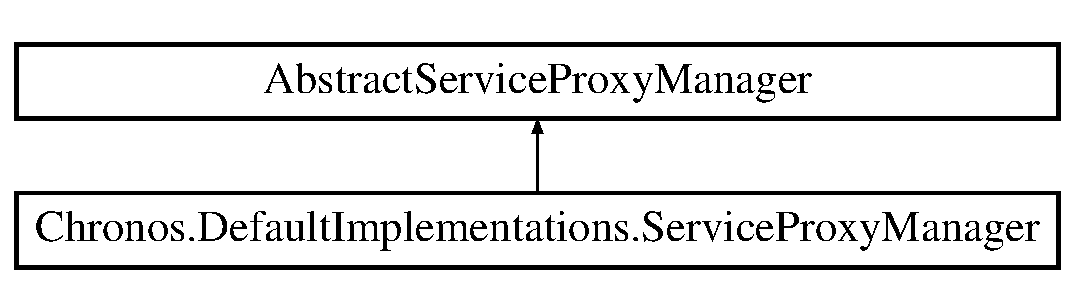
\includegraphics[height=2.000000cm]{classChronos_1_1DefaultImplementations_1_1ServiceProxyManager}
\end{center}
\end{figure}
\subsection*{Public Member Functions}
\begin{DoxyCompactItemize}
\item 
def {\bfseries \+\_\+\+\_\+init\+\_\+\+\_\+} (self, infrastructure\+Provider, kwargs)
\item 
def {\bfseries Dispose} (self)
\item 
def {\bfseries Connect} (self)
\item 
def {\bfseries Disconnect} (self)
\end{DoxyCompactItemize}
\subsection*{Public Attributes}
\begin{DoxyCompactItemize}
\item 
{\bfseries service\+Endpoint}
\item 
{\bfseries client}
\end{DoxyCompactItemize}


The documentation for this class was generated from the following file\+:\begin{DoxyCompactItemize}
\item 
Chronos/Default\+Implementations.\+py\end{DoxyCompactItemize}

\hypertarget{classChronos_1_1DefaultImplementations_1_1WriteAggregateLogic}{}\section{Chronos.\+Default\+Implementations.\+Write\+Aggregate\+Logic Class Reference}
\label{classChronos_1_1DefaultImplementations_1_1WriteAggregateLogic}\index{Chronos.\+Default\+Implementations.\+Write\+Aggregate\+Logic@{Chronos.\+Default\+Implementations.\+Write\+Aggregate\+Logic}}


A Lua script for atmoic updating of Aggregate\+Logic information.  


Inheritance diagram for Chronos.\+Default\+Implementations.\+Write\+Aggregate\+Logic\+:\begin{figure}[H]
\begin{center}
\leavevmode
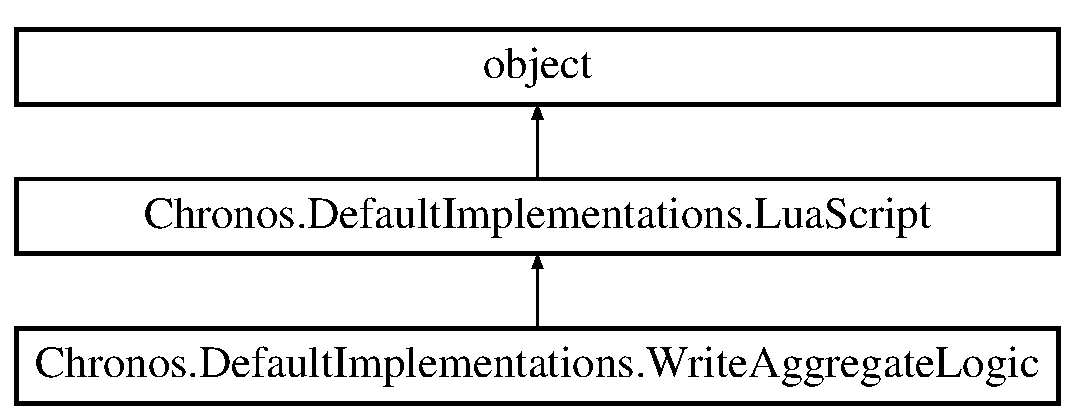
\includegraphics[height=3.000000cm]{classChronos_1_1DefaultImplementations_1_1WriteAggregateLogic}
\end{center}
\end{figure}
\subsection*{Public Member Functions}
\begin{DoxyCompactItemize}
\item 
def {\bfseries \+\_\+\+\_\+init\+\_\+\+\_\+} (self, logic\+Id\+Key, logic\+Key, aggregate\+Logic)
\item 
def {\bfseries Parse\+Redis\+Result} (self, redis\+Result)
\end{DoxyCompactItemize}
\subsection*{Static Public Attributes}
\begin{DoxyCompactItemize}
\item 
string {\bfseries Logic\+Lua\+Script}
\end{DoxyCompactItemize}
\subsection*{Additional Inherited Members}


\subsection{Detailed Description}
A Lua script for atmoic updating of Aggregate\+Logic information. 

The documentation for this class was generated from the following file\+:\begin{DoxyCompactItemize}
\item 
Chronos/Default\+Implementations.\+py\end{DoxyCompactItemize}

\hypertarget{classChronos_1_1Dependency_1_1AggregateSynchronizationManager}{}\section{Chronos.\+Dependency.\+Aggregate\+Synchronization\+Manager Class Reference}
\label{classChronos_1_1Dependency_1_1AggregateSynchronizationManager}\index{Chronos.\+Dependency.\+Aggregate\+Synchronization\+Manager@{Chronos.\+Dependency.\+Aggregate\+Synchronization\+Manager}}


Orchestrates a single-\/depth dependency tree of \hyperlink{classChronos_1_1Gateway_1_1ChronosProcess}{Chronos\+::\+Gateway\+::\+Chronos\+Process} instances.  


Inheritance diagram for Chronos.\+Dependency.\+Aggregate\+Synchronization\+Manager\+:\begin{figure}[H]
\begin{center}
\leavevmode
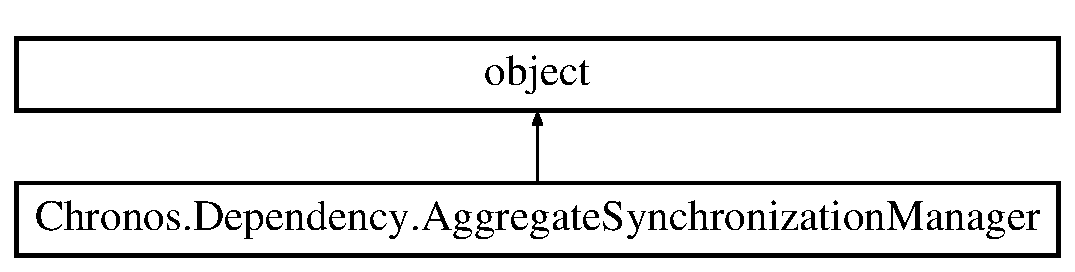
\includegraphics[height=2.000000cm]{classChronos_1_1Dependency_1_1AggregateSynchronizationManager}
\end{center}
\end{figure}
\subsection*{Public Member Functions}
\begin{DoxyCompactItemize}
\item 
def {\bfseries \+\_\+\+\_\+init\+\_\+\+\_\+} (self)
\item 
def \hyperlink{group__Chronos_gafe9e8666dcee9ec3f8e73f3ff92e2ded}{Add\+Synchronization\+Proxy} (self, name, proxy, dependencies)
\begin{DoxyCompactList}\small\item\em Adds a proxy for the provided Aggregate to the synchronization manager for later assignment. \end{DoxyCompactList}\item 
def \hyperlink{group__Chronos_gab57bfb327255df20320cc3e8f9a126c6}{Delete\+Synchronization\+Proxy} (self, name)
\begin{DoxyCompactList}\small\item\em Deletes the proxy for the provided Aggregate from the synchronization manager and all dependents. \end{DoxyCompactList}\end{DoxyCompactItemize}
\subsection*{Public Attributes}
\begin{DoxyCompactItemize}
\item 
{\bfseries aggregate\+Proxies}
\item 
{\bfseries reverse\+Dependency\+Mapping}
\item 
{\bfseries lock}
\end{DoxyCompactItemize}


\subsection{Detailed Description}
Orchestrates a single-\/depth dependency tree of \hyperlink{classChronos_1_1Gateway_1_1ChronosProcess}{Chronos\+::\+Gateway\+::\+Chronos\+Process} instances. 

The primary purpose of this class is to ensure that instances can be registered in any order; as long as all dependencies are registered before an event must be processed, the dependencies will be properly resolved. 

The documentation for this class was generated from the following file\+:\begin{DoxyCompactItemize}
\item 
Chronos/\hyperlink{Dependency_8py}{Dependency.\+py}\end{DoxyCompactItemize}

\hypertarget{classChronos_1_1Dependency_1_1ChronosProcessSynchronizer}{}\section{Chronos.\+Dependency.\+Chronos\+Process\+Synchronizer Class Reference}
\label{classChronos_1_1Dependency_1_1ChronosProcessSynchronizer}\index{Chronos.\+Dependency.\+Chronos\+Process\+Synchronizer@{Chronos.\+Dependency.\+Chronos\+Process\+Synchronizer}}


A utility class that encapsulates remote synchronization logic.  


Inheritance diagram for Chronos.\+Dependency.\+Chronos\+Process\+Synchronizer\+:\begin{figure}[H]
\begin{center}
\leavevmode
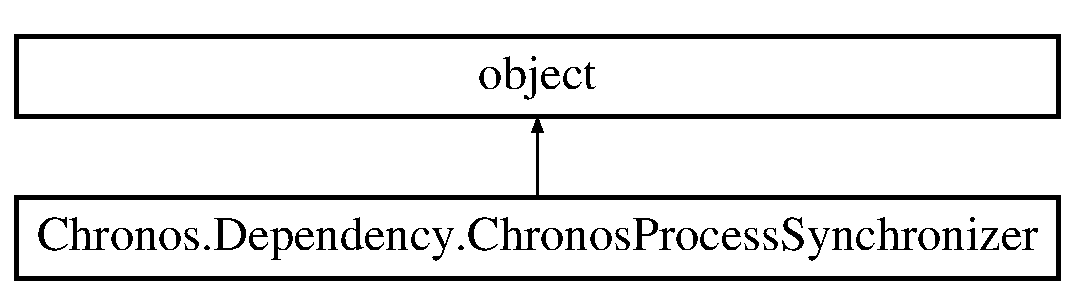
\includegraphics[height=2.000000cm]{classChronos_1_1Dependency_1_1ChronosProcessSynchronizer}
\end{center}
\end{figure}
\subsection*{Public Member Functions}
\begin{DoxyCompactItemize}
\item 
def {\bfseries \+\_\+\+\_\+init\+\_\+\+\_\+} (self)
\item 
def \hyperlink{group__Chronos_gaa5b77aa034528a45a2ea7ae04b430a2e}{Assign\+Synchronization\+Proxy} (self, aggregate\+Name, proxy)
\begin{DoxyCompactList}\small\item\em Adds a proxy to the internal registry for future use. \end{DoxyCompactList}\item 
def \hyperlink{group__Chronos_gaaf20aa3e37294492cf6f320d49ff64f2}{Delete\+Synchronization\+Proxy} (self, aggregate\+Name)
\begin{DoxyCompactList}\small\item\em Removes a proxy from the internal registry. \end{DoxyCompactList}\item 
def \hyperlink{group__Chronos_gad0ed4fb65d7d916312cd89e03a3c997a}{Acquire\+Dependencies} (self, aggregate, event)
\begin{DoxyCompactList}\small\item\em Acquires remote locks on all dependencies required by {\ttfamily event}. \end{DoxyCompactList}\item 
def \hyperlink{group__Chronos_ga461ce8c35896b5ebe0e18f3a76226c98}{Release\+Dependencies} (self)
\begin{DoxyCompactList}\small\item\em Releases all remote locks currently held by this instance. \end{DoxyCompactList}\end{DoxyCompactItemize}
\subsection*{Public Attributes}
\begin{DoxyCompactItemize}
\item 
{\bfseries synchronization\+Proxies}
\item 
{\bfseries remote\+Locks}
\end{DoxyCompactItemize}


\subsection{Detailed Description}
A utility class that encapsulates remote synchronization logic. 

This class is meant for use by \hyperlink{classChronos_1_1Gateway_1_1ChronosProcess}{Chronos\+::\+Gateway\+::\+Chronos\+Process}. 

The documentation for this class was generated from the following file\+:\begin{DoxyCompactItemize}
\item 
Chronos/\hyperlink{Dependency_8py}{Dependency.\+py}\end{DoxyCompactItemize}

\hypertarget{classChronos_1_1Dependency_1_1CircularReferenceException}{}\section{Chronos.\+Dependency.\+Circular\+Reference\+Exception Class Reference}
\label{classChronos_1_1Dependency_1_1CircularReferenceException}\index{Chronos.\+Dependency.\+Circular\+Reference\+Exception@{Chronos.\+Dependency.\+Circular\+Reference\+Exception}}
Inheritance diagram for Chronos.\+Dependency.\+Circular\+Reference\+Exception\+:\begin{figure}[H]
\begin{center}
\leavevmode
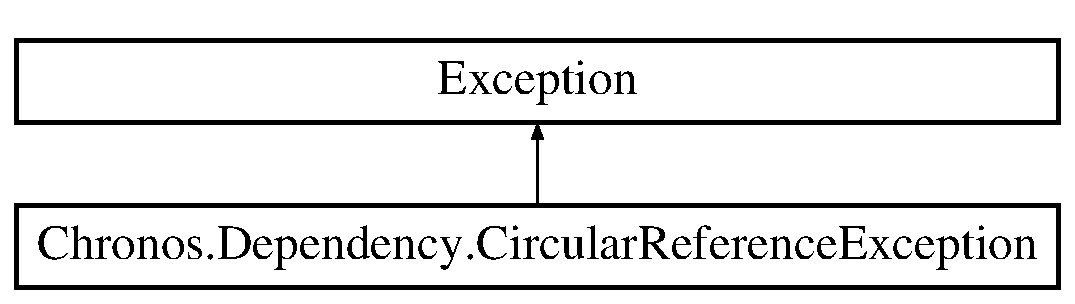
\includegraphics[height=2.000000cm]{classChronos_1_1Dependency_1_1CircularReferenceException}
\end{center}
\end{figure}


The documentation for this class was generated from the following file\+:\begin{DoxyCompactItemize}
\item 
Chronos/\hyperlink{Dependency_8py}{Dependency.\+py}\end{DoxyCompactItemize}

\hypertarget{classChronos_1_1Dependency_1_1DependenciesNotReleased}{}\section{Chronos.\+Dependency.\+Dependencies\+Not\+Released Class Reference}
\label{classChronos_1_1Dependency_1_1DependenciesNotReleased}\index{Chronos.\+Dependency.\+Dependencies\+Not\+Released@{Chronos.\+Dependency.\+Dependencies\+Not\+Released}}
Inheritance diagram for Chronos.\+Dependency.\+Dependencies\+Not\+Released\+:\begin{figure}[H]
\begin{center}
\leavevmode
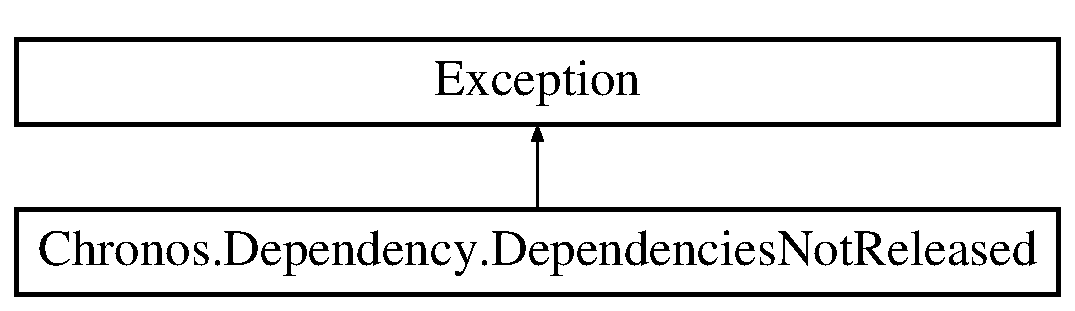
\includegraphics[height=2.000000cm]{classChronos_1_1Dependency_1_1DependenciesNotReleased}
\end{center}
\end{figure}


The documentation for this class was generated from the following file\+:\begin{DoxyCompactItemize}
\item 
Chronos/\hyperlink{Dependency_8py}{Dependency.\+py}\end{DoxyCompactItemize}

\hypertarget{classChronos_1_1Dependency_1_1dependent__upon}{}\section{Chronos.\+Dependency.\+dependent\+\_\+upon Class Reference}
\label{classChronos_1_1Dependency_1_1dependent__upon}\index{Chronos.\+Dependency.\+dependent\+\_\+upon@{Chronos.\+Dependency.\+dependent\+\_\+upon}}


An optional class decorator for use with \hyperlink{classChronos_1_1Core_1_1Event}{Chronos\+::\+Core\+::\+Event} subclasses specifying an external dependency on another Aggregate instance.  


Inheritance diagram for Chronos.\+Dependency.\+dependent\+\_\+upon\+:\begin{figure}[H]
\begin{center}
\leavevmode
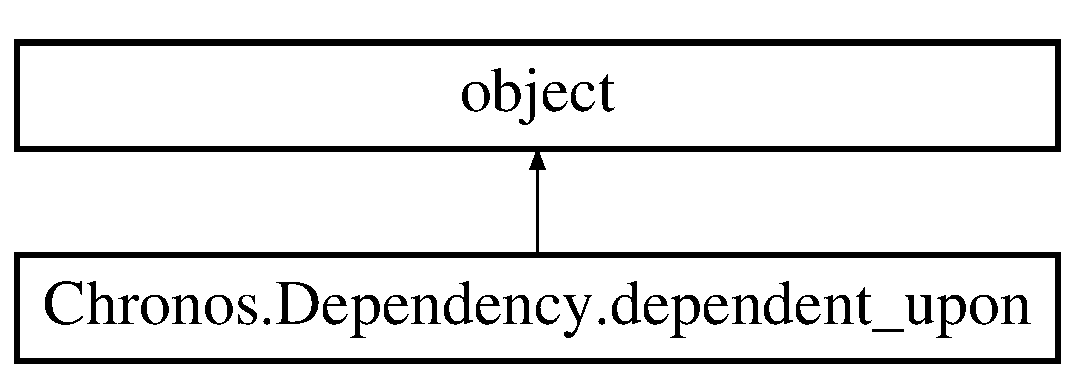
\includegraphics[height=2.000000cm]{classChronos_1_1Dependency_1_1dependent__upon}
\end{center}
\end{figure}


\subsection{Detailed Description}
An optional class decorator for use with \hyperlink{classChronos_1_1Core_1_1Event}{Chronos\+::\+Core\+::\+Event} subclasses specifying an external dependency on another Aggregate instance. 

Use of this decorator implies that instances of the decorated Event can only be processed after acquiring a lock on an external dependency. If the external dependency is unavailable (or cannot be resolved), then the Event will fail processing without attempting to execute its internal logic. 

The documentation for this class was generated from the following file\+:\begin{DoxyCompactItemize}
\item 
Chronos/\hyperlink{Dependency_8py}{Dependency.\+py}\end{DoxyCompactItemize}

\hypertarget{classChronos_1_1Dependency_1_1MissingDependency}{}\section{Chronos.\+Dependency.\+Missing\+Dependency Class Reference}
\label{classChronos_1_1Dependency_1_1MissingDependency}\index{Chronos.\+Dependency.\+Missing\+Dependency@{Chronos.\+Dependency.\+Missing\+Dependency}}
Inheritance diagram for Chronos.\+Dependency.\+Missing\+Dependency\+:\begin{figure}[H]
\begin{center}
\leavevmode
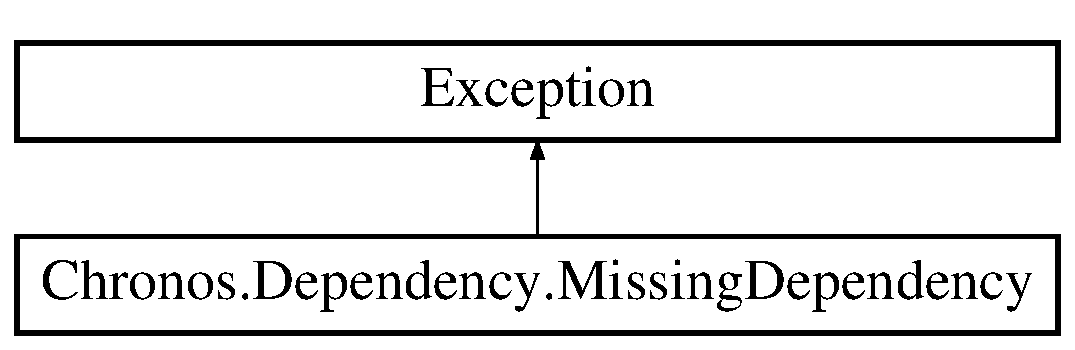
\includegraphics[height=2.000000cm]{classChronos_1_1Dependency_1_1MissingDependency}
\end{center}
\end{figure}


The documentation for this class was generated from the following file\+:\begin{DoxyCompactItemize}
\item 
Chronos/\hyperlink{Dependency_8py}{Dependency.\+py}\end{DoxyCompactItemize}

\hypertarget{classChronos_1_1EventLogger_1_1BTFileHandler}{}\section{Chronos.\+Event\+Logger.\+B\+T\+File\+Handler Class Reference}
\label{classChronos_1_1EventLogger_1_1BTFileHandler}\index{Chronos.\+Event\+Logger.\+B\+T\+File\+Handler@{Chronos.\+Event\+Logger.\+B\+T\+File\+Handler}}


File\+Handler wrapper to prevent users from having to import logging.  


Inheritance diagram for Chronos.\+Event\+Logger.\+B\+T\+File\+Handler\+:\begin{figure}[H]
\begin{center}
\leavevmode
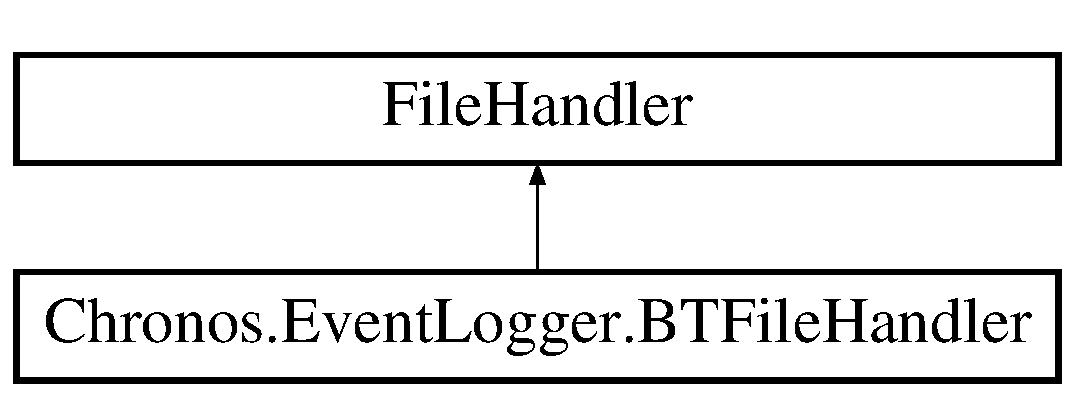
\includegraphics[height=2.000000cm]{classChronos_1_1EventLogger_1_1BTFileHandler}
\end{center}
\end{figure}
\subsection*{Public Member Functions}
\begin{DoxyCompactItemize}
\item 
def {\bfseries \+\_\+\+\_\+init\+\_\+\+\_\+} (self, filename, mode=\textquotesingle{}a\textquotesingle{}, encoding=None, delay=False)
\end{DoxyCompactItemize}
\subsection*{Static Public Member Functions}
\begin{DoxyCompactItemize}
\item 
def {\bfseries Create\+Path} (path)
\end{DoxyCompactItemize}


\subsection{Detailed Description}
File\+Handler wrapper to prevent users from having to import logging. 

The documentation for this class was generated from the following file\+:\begin{DoxyCompactItemize}
\item 
Chronos/Event\+Logger.\+py\end{DoxyCompactItemize}

\hypertarget{classChronos_1_1EventLogger_1_1BTNullHandler}{}\section{Chronos.\+Event\+Logger.\+B\+T\+Null\+Handler Class Reference}
\label{classChronos_1_1EventLogger_1_1BTNullHandler}\index{Chronos.\+Event\+Logger.\+B\+T\+Null\+Handler@{Chronos.\+Event\+Logger.\+B\+T\+Null\+Handler}}


Null\+Handler wrapper to prevent users from having to import logging.  


Inheritance diagram for Chronos.\+Event\+Logger.\+B\+T\+Null\+Handler\+:\begin{figure}[H]
\begin{center}
\leavevmode
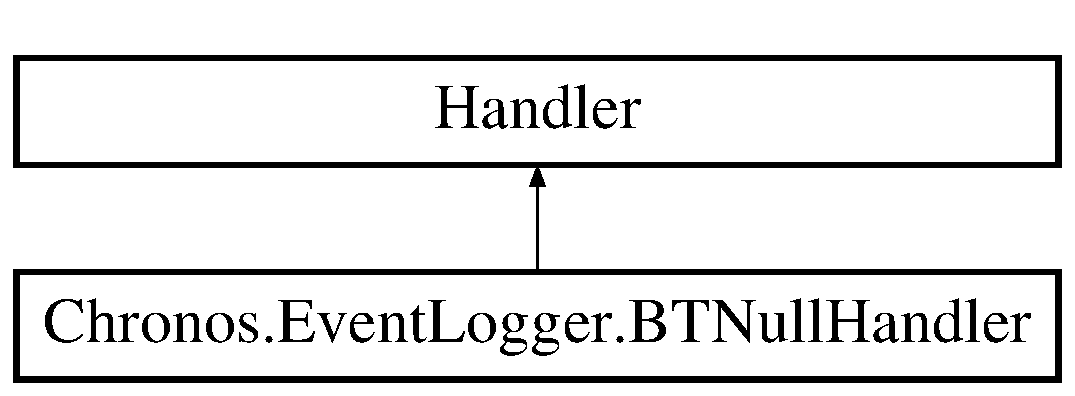
\includegraphics[height=2.000000cm]{classChronos_1_1EventLogger_1_1BTNullHandler}
\end{center}
\end{figure}
\subsection*{Public Member Functions}
\begin{DoxyCompactItemize}
\item 
def {\bfseries emit} (self, record)
\end{DoxyCompactItemize}


\subsection{Detailed Description}
Null\+Handler wrapper to prevent users from having to import logging. 

The documentation for this class was generated from the following file\+:\begin{DoxyCompactItemize}
\item 
Chronos/Event\+Logger.\+py\end{DoxyCompactItemize}

\hypertarget{classChronos_1_1EventLogger_1_1BTStreamHandler}{}\section{Chronos.\+Event\+Logger.\+B\+T\+Stream\+Handler Class Reference}
\label{classChronos_1_1EventLogger_1_1BTStreamHandler}\index{Chronos.\+Event\+Logger.\+B\+T\+Stream\+Handler@{Chronos.\+Event\+Logger.\+B\+T\+Stream\+Handler}}


Stream\+Handler wrapper to prevent users from having to import logging.  


Inheritance diagram for Chronos.\+Event\+Logger.\+B\+T\+Stream\+Handler\+:\begin{figure}[H]
\begin{center}
\leavevmode
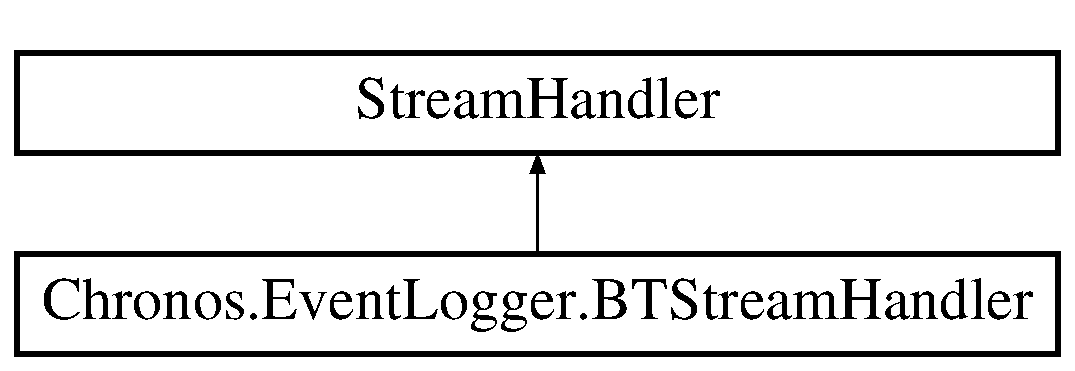
\includegraphics[height=2.000000cm]{classChronos_1_1EventLogger_1_1BTStreamHandler}
\end{center}
\end{figure}
\subsection*{Public Member Functions}
\begin{DoxyCompactItemize}
\item 
def {\bfseries \+\_\+\+\_\+init\+\_\+\+\_\+} (self, stream=None)
\end{DoxyCompactItemize}


\subsection{Detailed Description}
Stream\+Handler wrapper to prevent users from having to import logging. 

The documentation for this class was generated from the following file\+:\begin{DoxyCompactItemize}
\item 
Chronos/Event\+Logger.\+py\end{DoxyCompactItemize}

\hypertarget{classChronos_1_1EventLogger_1_1EventLogger}{}\section{Chronos.\+Event\+Logger.\+Event\+Logger Class Reference}
\label{classChronos_1_1EventLogger_1_1EventLogger}\index{Chronos.\+Event\+Logger.\+Event\+Logger@{Chronos.\+Event\+Logger.\+Event\+Logger}}


Handles logging of events that should be consumed by Splunk.  


Inheritance diagram for Chronos.\+Event\+Logger.\+Event\+Logger\+:\begin{figure}[H]
\begin{center}
\leavevmode
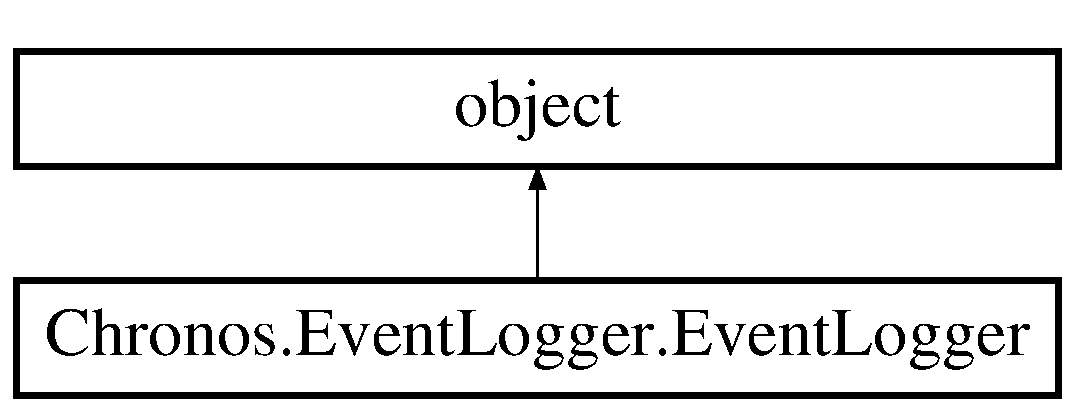
\includegraphics[height=2.000000cm]{classChronos_1_1EventLogger_1_1EventLogger}
\end{center}
\end{figure}
\subsection*{Public Member Functions}
\begin{DoxyCompactItemize}
\item 
def \hyperlink{group__PyInfrastructure_ga909b4948081a7832e704215ec484dea4}{\+\_\+\+\_\+init\+\_\+\+\_\+} (self, application, log\+File\+Path, firm, info\+Sys, who\+AmI, where\+AmI, settings, handlers)
\begin{DoxyCompactList}\small\item\em This constructor should only be called by an initialization function. \end{DoxyCompactList}\item 
def {\bfseries Set\+Handlers} (self, handlers)
\item 
def {\bfseries Reset\+Handlers} (self)
\item 
def {\bfseries Set\+Level} (self, level)
\end{DoxyCompactItemize}
\subsection*{Static Public Member Functions}
\begin{DoxyCompactItemize}
\item 
def {\bfseries Initialize\+Logger} (firm=None, info\+Sys=None, who\+AmI=None, where\+AmI=None, application=None, directory=None, settings=\hyperlink{classChronos_1_1EventLogger_1_1PersistentLoggerSettings}{Persistent\+Logger\+Settings}(), handler=None)
\item 
def {\bfseries Deinitialize\+Logger} ()
\item 
def {\bfseries Set\+Global\+Level} (level)
\item 
def \hyperlink{group__PyInfrastructure_ga22b169d02d02c1c7db9de09d26cf1319}{Get\+Logger} ()
\begin{DoxyCompactList}\small\item\em Gets the current \hyperlink{classChronos_1_1EventLogger_1_1EventLogger}{Event\+Logger} object. \end{DoxyCompactList}\item 
def {\bfseries Log\+Critical} (component, module, function, title, reason=None, tags=None)
\item 
def {\bfseries Log\+Error} (component, module, function, title, reason=None, tags=None)
\item 
def {\bfseries Log\+Warning} (component, module, function, title, reason=None, tags=None)
\item 
def {\bfseries Log\+Information} (component, module, function, title, reason=None, tags=None)
\item 
def {\bfseries Log\+Debug} (component, module, function, title, reason=None, tags=None)
\item 
def {\bfseries Log\+Exception} (component, module, function, title=None, reason=None, tags=None)
\item 
def {\bfseries Log\+Critical\+Auto} (obj, title, reason=None, tags=None)
\item 
def {\bfseries Log\+Error\+Auto} (obj, title, reason=None, tags=None)
\item 
def {\bfseries Log\+Warning\+Auto} (obj, title, reason=None, tags=None)
\item 
def {\bfseries Log\+Information\+Auto} (obj, title, reason=None, tags=None)
\item 
def {\bfseries Log\+Debug\+Auto} (obj, title, reason=None, tags=None)
\item 
def {\bfseries Log\+Exception\+Auto} (obj, title=None, reason=None, tags=None)
\end{DoxyCompactItemize}
\subsection*{Public Attributes}
\begin{DoxyCompactItemize}
\item 
{\bfseries application}
\item 
{\bfseries log\+File\+Path}
\item 
{\bfseries firm}
\item 
{\bfseries info\+Sys}
\item 
{\bfseries who\+AmI}
\item 
{\bfseries where\+AmI}
\item 
{\bfseries settings}
\item 
{\bfseries handlers}
\item 
{\bfseries logger}
\end{DoxyCompactItemize}
\subsection*{Static Public Attributes}
\begin{DoxyCompactItemize}
\item 
bool {\bfseries Initialized} = False
\item 
{\bfseries Logger} = None
\end{DoxyCompactItemize}


\subsection{Detailed Description}
Handles logging of events that should be consumed by Splunk. 

A single static \hyperlink{classChronos_1_1EventLogger_1_1EventLogger}{Event\+Logger} instance should exist for each application, created via one of the initialization functions. 

The documentation for this class was generated from the following file\+:\begin{DoxyCompactItemize}
\item 
Chronos/Event\+Logger.\+py\end{DoxyCompactItemize}

\hypertarget{classChronos_1_1EventLogger_1_1EventLoggerException}{}\section{Chronos.\+Event\+Logger.\+Event\+Logger\+Exception Class Reference}
\label{classChronos_1_1EventLogger_1_1EventLoggerException}\index{Chronos.\+Event\+Logger.\+Event\+Logger\+Exception@{Chronos.\+Event\+Logger.\+Event\+Logger\+Exception}}


Singular exception to be thrown from \hyperlink{classChronos_1_1EventLogger_1_1EventLogger}{Event\+Logger} functions.  


Inheritance diagram for Chronos.\+Event\+Logger.\+Event\+Logger\+Exception\+:\begin{figure}[H]
\begin{center}
\leavevmode
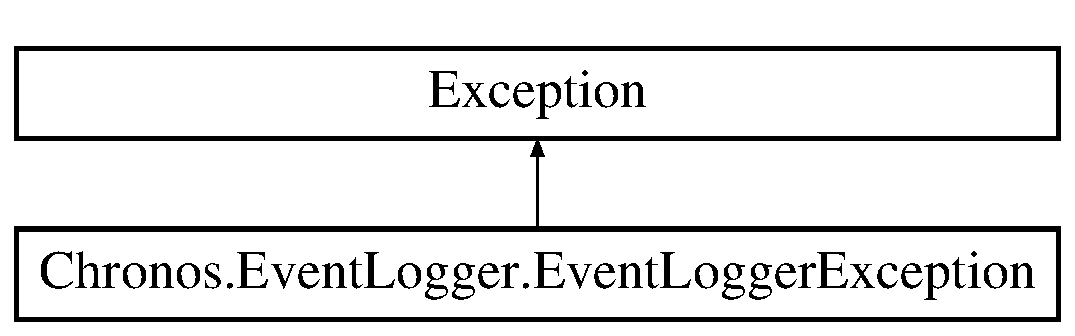
\includegraphics[height=2.000000cm]{classChronos_1_1EventLogger_1_1EventLoggerException}
\end{center}
\end{figure}


\subsection{Detailed Description}
Singular exception to be thrown from \hyperlink{classChronos_1_1EventLogger_1_1EventLogger}{Event\+Logger} functions. 

The documentation for this class was generated from the following file\+:\begin{DoxyCompactItemize}
\item 
Chronos/Event\+Logger.\+py\end{DoxyCompactItemize}

\hypertarget{classChronos_1_1EventLogger_1_1LoggerLevel}{}\section{Chronos.\+Event\+Logger.\+Logger\+Level Class Reference}
\label{classChronos_1_1EventLogger_1_1LoggerLevel}\index{Chronos.\+Event\+Logger.\+Logger\+Level@{Chronos.\+Event\+Logger.\+Logger\+Level}}


Level wrapper to prevent users from having to import logging.  


Inheritance diagram for Chronos.\+Event\+Logger.\+Logger\+Level\+:\begin{figure}[H]
\begin{center}
\leavevmode
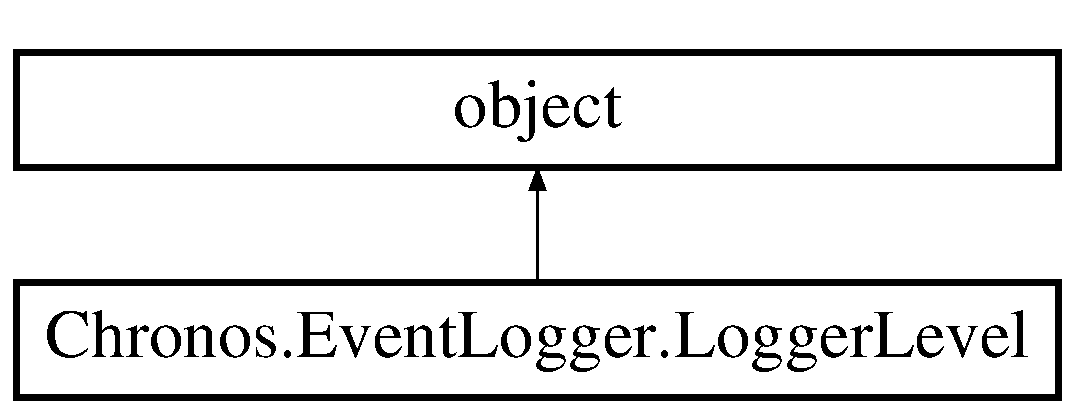
\includegraphics[height=2.000000cm]{classChronos_1_1EventLogger_1_1LoggerLevel}
\end{center}
\end{figure}
\subsection*{Static Public Attributes}
\begin{DoxyCompactItemize}
\item 
{\bfseries Critical} = logging.\+C\+R\+I\+T\+I\+C\+AL
\item 
{\bfseries Error} = logging.\+E\+R\+R\+OR
\item 
{\bfseries Warn} = logging.\+W\+A\+RN
\item 
{\bfseries Info} = logging.\+I\+N\+FO
\item 
{\bfseries Debug} = logging.\+D\+E\+B\+UG
\item 
{\bfseries Not\+Set} = logging.\+N\+O\+T\+S\+ET
\end{DoxyCompactItemize}


\subsection{Detailed Description}
Level wrapper to prevent users from having to import logging. 

The documentation for this class was generated from the following file\+:\begin{DoxyCompactItemize}
\item 
Chronos/Event\+Logger.\+py\end{DoxyCompactItemize}

\hypertarget{classChronos_1_1EventLogger_1_1PersistentLoggerSettings}{}\section{Chronos.\+Event\+Logger.\+Persistent\+Logger\+Settings Class Reference}
\label{classChronos_1_1EventLogger_1_1PersistentLoggerSettings}\index{Chronos.\+Event\+Logger.\+Persistent\+Logger\+Settings@{Chronos.\+Event\+Logger.\+Persistent\+Logger\+Settings}}


Settings that will be applied to every log written by the \hyperlink{classChronos_1_1EventLogger_1_1EventLogger}{Event\+Logger} once it\textquotesingle{}s initialized.  


Inheritance diagram for Chronos.\+Event\+Logger.\+Persistent\+Logger\+Settings\+:\begin{figure}[H]
\begin{center}
\leavevmode
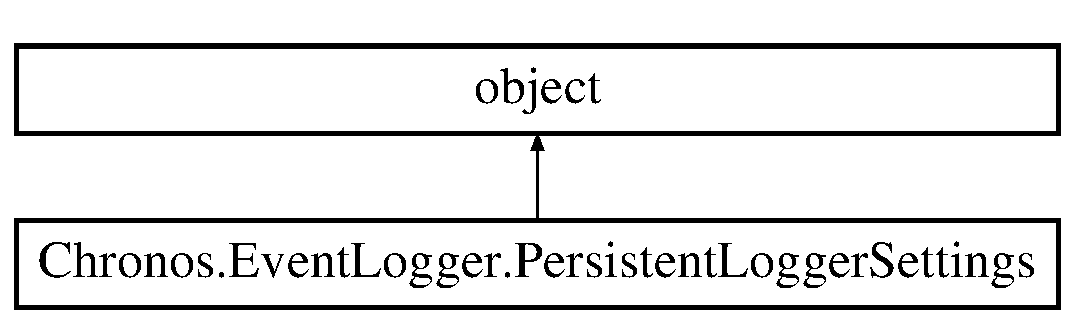
\includegraphics[height=2.000000cm]{classChronos_1_1EventLogger_1_1PersistentLoggerSettings}
\end{center}
\end{figure}
\subsection*{Public Member Functions}
\begin{DoxyCompactItemize}
\item 
def {\bfseries \+\_\+\+\_\+init\+\_\+\+\_\+} (self, level=Logger\+Level.\+Info, tags=None, log\+Format=\textquotesingle{}\%(asctime) s U\+TC;\%(message) s\textquotesingle{}, date\+Format=None)
\item 
def {\bfseries Add\+Tag} (self, key, value)
\item 
def {\bfseries Pop\+Tag} (self, key)
\item 
def {\bfseries Get\+Formatter} (self)
\end{DoxyCompactItemize}
\subsection*{Public Attributes}
\begin{DoxyCompactItemize}
\item 
{\bfseries level}
\item 
{\bfseries tags}
\item 
{\bfseries log\+Format}
\item 
{\bfseries date\+Format}
\end{DoxyCompactItemize}


\subsection{Detailed Description}
Settings that will be applied to every log written by the \hyperlink{classChronos_1_1EventLogger_1_1EventLogger}{Event\+Logger} once it\textquotesingle{}s initialized. 

The documentation for this class was generated from the following file\+:\begin{DoxyCompactItemize}
\item 
Chronos/Event\+Logger.\+py\end{DoxyCompactItemize}

\hypertarget{classChronos_1_1EventLogger_1_1PreciseTimeLoggingFormatter}{}\section{Chronos.\+Event\+Logger.\+Precise\+Time\+Logging\+Formatter Class Reference}
\label{classChronos_1_1EventLogger_1_1PreciseTimeLoggingFormatter}\index{Chronos.\+Event\+Logger.\+Precise\+Time\+Logging\+Formatter@{Chronos.\+Event\+Logger.\+Precise\+Time\+Logging\+Formatter}}
Inheritance diagram for Chronos.\+Event\+Logger.\+Precise\+Time\+Logging\+Formatter\+:\begin{figure}[H]
\begin{center}
\leavevmode
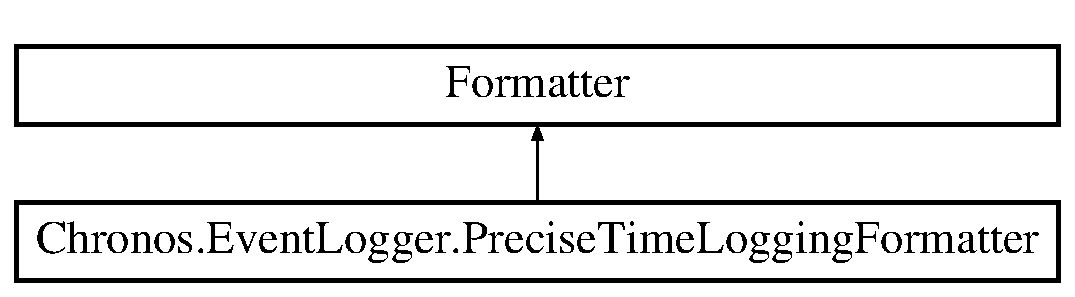
\includegraphics[height=2.000000cm]{classChronos_1_1EventLogger_1_1PreciseTimeLoggingFormatter}
\end{center}
\end{figure}
\subsection*{Public Member Functions}
\begin{DoxyCompactItemize}
\item 
def {\bfseries format\+Time} (self, record, datefmt=None)
\end{DoxyCompactItemize}


The documentation for this class was generated from the following file\+:\begin{DoxyCompactItemize}
\item 
Chronos/Event\+Logger.\+py\end{DoxyCompactItemize}

\hypertarget{classChronos_1_1EventLogger_1_1UnitializedEventLogger}{}\section{Chronos.\+Event\+Logger.\+Unitialized\+Event\+Logger Class Reference}
\label{classChronos_1_1EventLogger_1_1UnitializedEventLogger}\index{Chronos.\+Event\+Logger.\+Unitialized\+Event\+Logger@{Chronos.\+Event\+Logger.\+Unitialized\+Event\+Logger}}
Inheritance diagram for Chronos.\+Event\+Logger.\+Unitialized\+Event\+Logger\+:\begin{figure}[H]
\begin{center}
\leavevmode
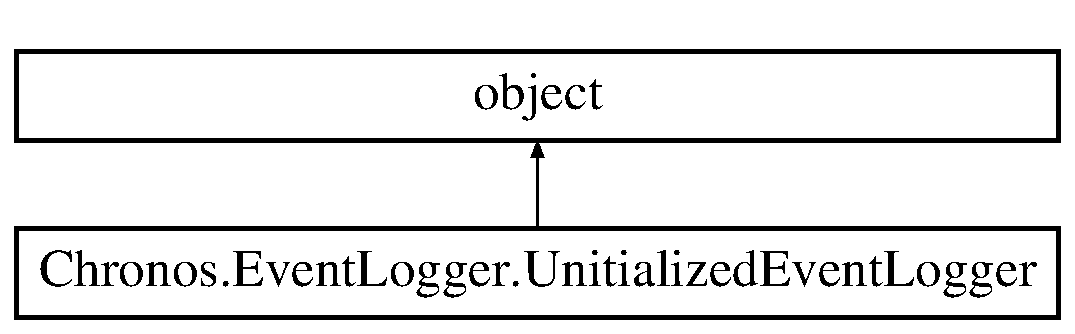
\includegraphics[height=2.000000cm]{classChronos_1_1EventLogger_1_1UnitializedEventLogger}
\end{center}
\end{figure}


The documentation for this class was generated from the following file\+:\begin{DoxyCompactItemize}
\item 
Chronos/Event\+Logger.\+py\end{DoxyCompactItemize}

\hypertarget{classChronos_1_1Gateway_1_1ChronosGateway}{}\section{Chronos.\+Gateway.\+Chronos\+Gateway Class Reference}
\label{classChronos_1_1Gateway_1_1ChronosGateway}\index{Chronos.\+Gateway.\+Chronos\+Gateway@{Chronos.\+Gateway.\+Chronos\+Gateway}}


The main server implementation.  


Inheritance diagram for Chronos.\+Gateway.\+Chronos\+Gateway\+:\begin{figure}[H]
\begin{center}
\leavevmode
\includegraphics[height=2.000000cm]{classChronos_1_1Gateway_1_1ChronosGateway}
\end{center}
\end{figure}
\subsection*{Public Member Functions}
\begin{DoxyCompactItemize}
\item 
def {\bfseries \+\_\+\+\_\+init\+\_\+\+\_\+} (self, event\+Store, synchronization\+Manager, core\+Provider\+Generator)
\item 
def \hyperlink{group__Chronos_ga6d1d412b8ee16cf3bf7be976a4041ced}{Load\+Registry} (self)
\begin{DoxyCompactList}\small\item\em If a previous instance of the \hyperlink{classChronos_1_1Gateway_1_1ChronosGateway}{Chronos\+Gateway} persisted registry information to disk, this method will re-\/register all previously registered aggregate logic. \end{DoxyCompactList}\item 
def \hyperlink{group__Chronos_ga20a6380c276ad93d3f59832c88b1b863}{Save\+Registry} (self)
\begin{DoxyCompactList}\small\item\em Persists registry information to disk for reloading upon gateway startup. \end{DoxyCompactList}\item 
def \hyperlink{group__Chronos_ga99107362643b72b54fdabf6d6d5ab0e9}{Register} (self, request)
\begin{DoxyCompactList}\small\item\em Compiles protobuf messages and Python logic for Aggregate registration, then updates the current state of the server. \end{DoxyCompactList}\item 
def \hyperlink{group__Chronos_ga4e8e260962d11dc692f37a03da88e48a}{Add\+Registry\+Item} (self, logic\+Version, module)
\begin{DoxyCompactList}\small\item\em Creates a new \hyperlink{classChronos_1_1Gateway_1_1ChronosProcessManager}{Chronos\+Process\+Manager} and \hyperlink{classChronos_1_1Gateway_1_1ChronosProcess}{Chronos\+Process} for the module created from a Chronos\+Registration\+Request. \end{DoxyCompactList}\item 
def \hyperlink{group__Chronos_ga62459e3c9eae9e1ea22841512298b40b}{Get\+Registry\+Item} (self, aggregate\+Name)
\begin{DoxyCompactList}\small\item\em Retrieves the \hyperlink{classChronos_1_1Gateway_1_1ChronosRegistryItem}{Chronos\+Registry\+Item} for the given aggregate. \end{DoxyCompactList}\item 
def \hyperlink{group__Chronos_gaf1f7b9953b7fd0e2ef47e55405c66acc}{Unregister} (self, aggregate\+Name)
\begin{DoxyCompactList}\small\item\em Shuts down the \hyperlink{classChronos_1_1Gateway_1_1ChronosProcessManager}{Chronos\+Process\+Manager} and \hyperlink{classChronos_1_1Gateway_1_1ChronosProcess}{Chronos\+Process} for the supplied aggregate. \end{DoxyCompactList}\item 
def \hyperlink{group__Chronos_ga9355f09e2f692b2d379033d69d5a02fa}{Check\+Status} (self, aggregate\+Name)
\begin{DoxyCompactList}\small\item\em Returns a Chronos\+Registration\+Response detailing the current status of {\ttfamily aggregate\+Name}. \end{DoxyCompactList}\item 
def \hyperlink{group__Chronos_gacbe9f7549ce9b5f11f2cb3d4dca74638}{Route\+Event} (self, request)
\begin{DoxyCompactList}\small\item\em Creates a Chronos\+Event\+Queue\+Item and enqueues it for processing by the correct \hyperlink{classChronos_1_1Gateway_1_1ChronosProcess}{Chronos\+Process} instance. \end{DoxyCompactList}\item 
def \hyperlink{group__Chronos_gaea90e7dc86d552e1e9f9b66d47858d37}{Route\+Event\+With\+Tag} (self, request)
\begin{DoxyCompactList}\small\item\em Creates a Chronos\+Event\+Queue\+Item and enqueues it for processing by the correct \hyperlink{classChronos_1_1Gateway_1_1ChronosProcess}{Chronos\+Process} instance. \end{DoxyCompactList}\item 
def \hyperlink{group__Chronos_gaa906b0081fb403254dc6fcc4d718629f}{Route\+Transaction} (self, transaction)
\begin{DoxyCompactList}\small\item\em Creates a Chronos\+Transaction\+Queue\+Item and enqueues it for processing by the correct \hyperlink{classChronos_1_1Gateway_1_1ChronosProcess}{Chronos\+Process} instance. \end{DoxyCompactList}\item 
def \hyperlink{group__Chronos_gab8200236e0e382a3f1fa576190267513}{Get\+All} (self, request)
\begin{DoxyCompactList}\small\item\em Retrieves all snapshots for the supplied Aggregate. \end{DoxyCompactList}\item 
def \hyperlink{group__Chronos_ga1dd0cc5ef184d3634b482e16bdfaaffe}{Get\+By\+Id} (self, request)
\begin{DoxyCompactList}\small\item\em Retrieves the snapshot for the supplied aggregate. \end{DoxyCompactList}\item 
def \hyperlink{group__Chronos_ga46ee58f34474277a9b54d3e1814c8115}{Get\+By\+Index} (self, request)
\begin{DoxyCompactList}\small\item\em Retrieves all snapshots for the supplied Aggregate that satisfy the supplied index key. \end{DoxyCompactList}\item 
def \hyperlink{group__Chronos_ga3abe9fb6af06ad9e1cce2a645624dbbe}{Get\+By\+Tag} (self, request)
\begin{DoxyCompactList}\small\item\em Retrieves the tagged snapshot corresponding to the given request. \end{DoxyCompactList}\item 
def \hyperlink{group__Chronos_ga66539ba88e0de9efc24890c09a720b7e}{Get\+Tags} (self, aggregate\+Name)
\begin{DoxyCompactList}\small\item\em Retrieves all tags for the provided Aggregate. \end{DoxyCompactList}\item 
def \hyperlink{group__Chronos_gafce09c1b25233cee3a27f22c1073896e}{Shutdown} (self)
\begin{DoxyCompactList}\small\item\em Shuts down all registered \hyperlink{classChronos_1_1Gateway_1_1ChronosProcessManager}{Chronos\+Process\+Manager} and \hyperlink{classChronos_1_1Gateway_1_1ChronosProcess}{Chronos\+Process} instances. \end{DoxyCompactList}\end{DoxyCompactItemize}
\subsection*{Static Public Member Functions}
\begin{DoxyCompactItemize}
\item 
def {\bfseries Create\+Registration\+Response} (error\+Message=\textquotesingle{}\textquotesingle{}, indexed\+Attributes=None)
\end{DoxyCompactItemize}
\subsection*{Public Attributes}
\begin{DoxyCompactItemize}
\item 
{\bfseries event\+Store}
\item 
{\bfseries synchronization\+Manager}
\item 
{\bfseries core\+Provider\+Generator}
\item 
{\bfseries logic\+Compiler}
\item 
{\bfseries statistics\+Logger}
\item 
{\bfseries request\+Id\+Lock}
\item 
{\bfseries registry\+Lock}
\item 
{\bfseries registry}
\item 
{\bfseries request\+Id\+Counter}
\end{DoxyCompactItemize}
\subsection*{Static Public Attributes}
\begin{DoxyCompactItemize}
\item 
string {\bfseries Registered\+Modules\+Path} = \textquotesingle{}modules.\+dat\textquotesingle{}
\end{DoxyCompactItemize}


\subsection{Detailed Description}
The main server implementation. 

The \hyperlink{classChronos_1_1Gateway_1_1ChronosGateway}{Chronos\+Gateway} handles registration of aggregate/event logic from clients and routes event/query requests to the proper \hyperlink{classChronos_1_1Gateway_1_1ChronosProcess}{Chronos\+Process}. 

The documentation for this class was generated from the following file\+:\begin{DoxyCompactItemize}
\item 
Chronos/\hyperlink{Gateway_8py}{Gateway.\+py}\end{DoxyCompactItemize}

\hypertarget{classChronos_1_1Gateway_1_1ChronosGatewayException}{}\section{Chronos.\+Gateway.\+Chronos\+Gateway\+Exception Class Reference}
\label{classChronos_1_1Gateway_1_1ChronosGatewayException}\index{Chronos.\+Gateway.\+Chronos\+Gateway\+Exception@{Chronos.\+Gateway.\+Chronos\+Gateway\+Exception}}


An Exception indicating that Chronos has encountered an error from which it is unable to recover.  


Inheritance diagram for Chronos.\+Gateway.\+Chronos\+Gateway\+Exception\+:\begin{figure}[H]
\begin{center}
\leavevmode
\includegraphics[height=2.000000cm]{classChronos_1_1Gateway_1_1ChronosGatewayException}
\end{center}
\end{figure}


\subsection{Detailed Description}
An Exception indicating that Chronos has encountered an error from which it is unable to recover. 

This Exception could be thrown due to network events, logic errors, or inconsistent state. 

The documentation for this class was generated from the following file\+:\begin{DoxyCompactItemize}
\item 
Chronos/\hyperlink{Gateway_8py}{Gateway.\+py}\end{DoxyCompactItemize}

\hypertarget{classChronos_1_1Gateway_1_1ChronosProcess}{}\section{Chronos.\+Gateway.\+Chronos\+Process Class Reference}
\label{classChronos_1_1Gateway_1_1ChronosProcess}\index{Chronos.\+Gateway.\+Chronos\+Process@{Chronos.\+Gateway.\+Chronos\+Process}}


The main logical component of the \hyperlink{classChronos_1_1Gateway_1_1ChronosGateway}{Chronos\+Gateway}.  


Inheritance diagram for Chronos.\+Gateway.\+Chronos\+Process\+:\begin{figure}[H]
\begin{center}
\leavevmode
\includegraphics[height=2.000000cm]{classChronos_1_1Gateway_1_1ChronosProcess}
\end{center}
\end{figure}
\subsection*{Public Member Functions}
\begin{DoxyCompactItemize}
\item 
def {\bfseries \+\_\+\+\_\+init\+\_\+\+\_\+} (self, aggregate\+Class, aggregate\+Registry, logic\+Version, core\+Provider\+Generator)
\item 
def \hyperlink{group__Chronos_gae5027792d4f78b27d2b2eed69eeae697}{Startup} (self)
\begin{DoxyCompactList}\small\item\em Creates the Chronos Core instances required for processing and starts the \hyperlink{group__Chronos_gaefd9a9f928112951d36eb314ec1d1ef2}{Chronos\+Process\+::\+Event\+Loop} in a background thread. \end{DoxyCompactList}\item 
def \hyperlink{group__Chronos_gaf7218fb21583767ca7bda97becef62fd}{Shutdown} (self)
\begin{DoxyCompactList}\small\item\em Cleans up the Chronos Core instances owned by this instance and stops the \hyperlink{group__Chronos_gaefd9a9f928112951d36eb314ec1d1ef2}{Chronos\+Process\+::\+Event\+Loop}. \end{DoxyCompactList}\item 
def {\bfseries Assign\+Synchronization\+Proxy} (self, aggregate\+Name, proxy)
\item 
def {\bfseries Delete\+Synchronization\+Proxy} (self, aggregate\+Name)
\item 
def \hyperlink{group__Chronos_ga8b8d1338ffabd17cbf64eac8998b8f4b}{Send\+Event} (self, event\+Queue\+Item)
\begin{DoxyCompactList}\small\item\em Enqueues in an event for processing. \end{DoxyCompactList}\item 
def \hyperlink{group__Chronos_gaefd9a9f928112951d36eb314ec1d1ef2}{Event\+Loop} (self)
\begin{DoxyCompactList}\small\item\em Event queue processing. \end{DoxyCompactList}\item 
def {\bfseries Begin} (self)
\item 
def {\bfseries Commit} (self)
\item 
def {\bfseries Rollback} (self)
\item 
def \hyperlink{group__Chronos_ga5ae412d35ae2277be0ea6d2013d12129}{Process\+Event} (self, event\+Queue\+Item)
\begin{DoxyCompactList}\small\item\em Determines the corresponding Python class to an event\+Type sent from a client and applies that type\textquotesingle{}s logic to the specified aggregate. \end{DoxyCompactList}\item 
def \hyperlink{group__Chronos_ga886ff894876545d6abaa78d677386d36}{Get\+Unexpired\+Aggregate} (self, event\+Queue\+Item)
\begin{DoxyCompactList}\small\item\em Attempts to retrieve the aggregate instance specified by event\+Queue\+Item. \end{DoxyCompactList}\item 
def {\bfseries Apply\+Event} (self, aggregate, event\+Queue\+Item)
\item 
def {\bfseries Acquire} (self, aggregate\+Id)
\item 
def {\bfseries Release} (self, aggregate\+Id)
\item 
def \hyperlink{group__Chronos_ga4c27fcd186b8c17d47b2d6a6d0dd8d55}{Query} (self, query\+Item)
\begin{DoxyCompactList}\small\item\em Processes a \hyperlink{classChronos_1_1Gateway_1_1ChronosQueryItem}{Chronos\+Query\+Item} to retrieve aggregate snapshots requested by a client. \end{DoxyCompactList}\item 
def {\bfseries Get\+All\+Tags} (self)
\item 
def {\bfseries Get\+By\+Tag} (self, tag, aggregate\+Id)
\end{DoxyCompactItemize}
\subsection*{Public Attributes}
\begin{DoxyCompactItemize}
\item 
{\bfseries aggregate\+Class}
\item 
{\bfseries aggregate\+Registry}
\item 
{\bfseries logic\+Version}
\item 
{\bfseries core\+Provider\+Generator}
\item 
{\bfseries process\+Synchronizer}
\item 
{\bfseries lock}
\item 
{\bfseries queue}
\item 
{\bfseries query\+Event}
\item 
{\bfseries is\+Running}
\item 
{\bfseries processing\+Thread}
\item 
{\bfseries core\+Provider}
\item 
{\bfseries index\+Store}
\item 
{\bfseries repository}
\item 
{\bfseries index}
\item 
{\bfseries processor}
\item 
{\bfseries max\+Request\+Id}
\end{DoxyCompactItemize}


\subsection{Detailed Description}
The main logical component of the \hyperlink{classChronos_1_1Gateway_1_1ChronosGateway}{Chronos\+Gateway}. 

Each aggregate that is registered with the service will have its own instance of \hyperlink{classChronos_1_1Gateway_1_1ChronosProcess}{Chronos\+Process}; each instance of \hyperlink{classChronos_1_1Gateway_1_1ChronosProcess}{Chronos\+Process} runs within its own physical process on the server.

\hyperlink{classChronos_1_1Gateway_1_1ChronosProcess}{Chronos\+Process} has three main pieces of functionality\+: asynchronous event queue processing, synchronous query handling, and tag management. Query hanlding is separated from the other operations and cannot affect writing. Tags can optionally be specified along with specific events (in which case a failing tag creation will fail the entire event).

This class is threadsafe and all exceptions should be logged and handled internally. 

The documentation for this class was generated from the following file\+:\begin{DoxyCompactItemize}
\item 
Chronos/\hyperlink{Gateway_8py}{Gateway.\+py}\end{DoxyCompactItemize}

\hypertarget{classChronos_1_1Gateway_1_1ChronosProcessManager}{}\section{Chronos.\+Gateway.\+Chronos\+Process\+Manager Class Reference}
\label{classChronos_1_1Gateway_1_1ChronosProcessManager}\index{Chronos.\+Gateway.\+Chronos\+Process\+Manager@{Chronos.\+Gateway.\+Chronos\+Process\+Manager}}


The multiprocessing.\+Manager that marshalls instances of \hyperlink{classChronos_1_1Gateway_1_1ChronosProcess}{Chronos\+Process} into their own physical processes on the server.  


Inheritance diagram for Chronos.\+Gateway.\+Chronos\+Process\+Manager\+:\begin{figure}[H]
\begin{center}
\leavevmode
\includegraphics[height=2.000000cm]{classChronos_1_1Gateway_1_1ChronosProcessManager}
\end{center}
\end{figure}
\subsection*{Public Member Functions}
\begin{DoxyCompactItemize}
\item 
def {\bfseries Shutdown} (self)
\end{DoxyCompactItemize}


\subsection{Detailed Description}
The multiprocessing.\+Manager that marshalls instances of \hyperlink{classChronos_1_1Gateway_1_1ChronosProcess}{Chronos\+Process} into their own physical processes on the server. 



The documentation for this class was generated from the following file\+:\begin{DoxyCompactItemize}
\item 
Chronos/\hyperlink{Gateway_8py}{Gateway.\+py}\end{DoxyCompactItemize}

\hypertarget{classChronos_1_1Gateway_1_1ChronosQueryItem}{}\section{Chronos.\+Gateway.\+Chronos\+Query\+Item Class Reference}
\label{classChronos_1_1Gateway_1_1ChronosQueryItem}\index{Chronos.\+Gateway.\+Chronos\+Query\+Item@{Chronos.\+Gateway.\+Chronos\+Query\+Item}}


A simple wrapper that unifies the three possible Chronos query types into a single request object.  


Inheritance diagram for Chronos.\+Gateway.\+Chronos\+Query\+Item\+:\begin{figure}[H]
\begin{center}
\leavevmode
\includegraphics[height=2.000000cm]{classChronos_1_1Gateway_1_1ChronosQueryItem}
\end{center}
\end{figure}
\subsection*{Public Member Functions}
\begin{DoxyCompactItemize}
\item 
def {\bfseries \+\_\+\+\_\+init\+\_\+\+\_\+} (self, aggregate\+Id=None, index\+Keys=None)
\end{DoxyCompactItemize}
\subsection*{Public Attributes}
\begin{DoxyCompactItemize}
\item 
{\bfseries aggregate\+Id}
\item 
{\bfseries index\+Keys}
\end{DoxyCompactItemize}


\subsection{Detailed Description}
A simple wrapper that unifies the three possible Chronos query types into a single request object. 

A \hyperlink{classChronos_1_1Gateway_1_1ChronosProcess}{Chronos\+Process} instance is able to use the \hyperlink{classChronos_1_1Gateway_1_1ChronosQueryItem}{Chronos\+Query\+Item} to return a subset of snapshots that a calling client is interested in. 

The documentation for this class was generated from the following file\+:\begin{DoxyCompactItemize}
\item 
Chronos/\hyperlink{Gateway_8py}{Gateway.\+py}\end{DoxyCompactItemize}

\hypertarget{classChronos_1_1Gateway_1_1ChronosRegistryItem}{}\section{Chronos.\+Gateway.\+Chronos\+Registry\+Item Class Reference}
\label{classChronos_1_1Gateway_1_1ChronosRegistryItem}\index{Chronos.\+Gateway.\+Chronos\+Registry\+Item@{Chronos.\+Gateway.\+Chronos\+Registry\+Item}}


Associates a \hyperlink{classChronos_1_1Gateway_1_1ChronosProcessManager}{Chronos\+Process\+Manager} with its \hyperlink{classChronos_1_1Gateway_1_1ChronosProcess}{Chronos\+Process} instance.  


Inheritance diagram for Chronos.\+Gateway.\+Chronos\+Registry\+Item\+:\begin{figure}[H]
\begin{center}
\leavevmode
\includegraphics[height=2.000000cm]{classChronos_1_1Gateway_1_1ChronosRegistryItem}
\end{center}
\end{figure}
\subsection*{Public Member Functions}
\begin{DoxyCompactItemize}
\item 
def {\bfseries \+\_\+\+\_\+init\+\_\+\+\_\+} (self)
\item 
def \hyperlink{group__Chronos_gae4d942c14fef0cc2abfc8ff9ca08eb14}{Startup} (self, manager, process, module)
\begin{DoxyCompactList}\small\item\em Starts the underlying \hyperlink{classChronos_1_1Gateway_1_1ChronosProcess}{Chronos\+Process}. \end{DoxyCompactList}\item 
def \hyperlink{group__Chronos_ga4094a3f48d548f9ed8c53ce14b900142}{Shutdown} (self)
\begin{DoxyCompactList}\small\item\em Shuts down both the underlying \hyperlink{classChronos_1_1Gateway_1_1ChronosProcess}{Chronos\+Process} and its manager. \end{DoxyCompactList}\end{DoxyCompactItemize}
\subsection*{Public Attributes}
\begin{DoxyCompactItemize}
\item 
{\bfseries lock}
\item 
{\bfseries is\+Running}
\item 
{\bfseries manager}
\item 
{\bfseries process}
\item 
{\bfseries module}
\end{DoxyCompactItemize}


\subsection{Detailed Description}
Associates a \hyperlink{classChronos_1_1Gateway_1_1ChronosProcessManager}{Chronos\+Process\+Manager} with its \hyperlink{classChronos_1_1Gateway_1_1ChronosProcess}{Chronos\+Process} instance. 

These items are retained by the \hyperlink{classChronos_1_1Gateway_1_1ChronosGateway}{Chronos\+Gateway} so that the gateway can be cleaned up in its entirety if necessary. 

The documentation for this class was generated from the following file\+:\begin{DoxyCompactItemize}
\item 
Chronos/\hyperlink{Gateway_8py}{Gateway.\+py}\end{DoxyCompactItemize}

\hypertarget{classChronos_1_1Gateway_1_1StatisticsLogger}{}\section{Chronos.\+Gateway.\+Statistics\+Logger Class Reference}
\label{classChronos_1_1Gateway_1_1StatisticsLogger}\index{Chronos.\+Gateway.\+Statistics\+Logger@{Chronos.\+Gateway.\+Statistics\+Logger}}


Aggregates and logs statistics about Chronos operations.  


Inheritance diagram for Chronos.\+Gateway.\+Statistics\+Logger\+:\begin{figure}[H]
\begin{center}
\leavevmode
\includegraphics[height=2.000000cm]{classChronos_1_1Gateway_1_1StatisticsLogger}
\end{center}
\end{figure}
\subsection*{Public Member Functions}
\begin{DoxyCompactItemize}
\item 
def {\bfseries \+\_\+\+\_\+init\+\_\+\+\_\+} (self)
\item 
def {\bfseries Log\+Aggregated\+Statistics} (self)
\item 
def {\bfseries Log\+Event} (self, aggregate\+Name, event\+Type)
\item 
def {\bfseries Log\+Query} (self, aggregate\+Name)
\item 
def {\bfseries Shutdown} (self)
\end{DoxyCompactItemize}
\subsection*{Public Attributes}
\begin{DoxyCompactItemize}
\item 
{\bfseries is\+Running}
\item 
{\bfseries aggregated\+Event\+Stats}
\item 
{\bfseries event\+Lock}
\item 
{\bfseries aggregated\+Query\+Stats}
\item 
{\bfseries query\+Lock}
\item 
{\bfseries last\+Log\+Time}
\item 
{\bfseries logging\+Thread}
\end{DoxyCompactItemize}
\subsection*{Static Public Attributes}
\begin{DoxyCompactItemize}
\item 
int {\bfseries Logging\+Interval} = 30
\end{DoxyCompactItemize}


\subsection{Detailed Description}
Aggregates and logs statistics about Chronos operations. 



The documentation for this class was generated from the following file\+:\begin{DoxyCompactItemize}
\item 
Chronos/\hyperlink{Gateway_8py}{Gateway.\+py}\end{DoxyCompactItemize}

\hypertarget{classChronos_1_1Infrastructure_1_1AbstractClientProxy}{}\section{Chronos.\+Infrastructure.\+Abstract\+Client\+Proxy Class Reference}
\label{classChronos_1_1Infrastructure_1_1AbstractClientProxy}\index{Chronos.\+Infrastructure.\+Abstract\+Client\+Proxy@{Chronos.\+Infrastructure.\+Abstract\+Client\+Proxy}}
Inheritance diagram for Chronos.\+Infrastructure.\+Abstract\+Client\+Proxy\+:\begin{figure}[H]
\begin{center}
\leavevmode
\includegraphics[height=3.000000cm]{classChronos_1_1Infrastructure_1_1AbstractClientProxy}
\end{center}
\end{figure}
\subsection*{Public Member Functions}
\begin{DoxyCompactItemize}
\item 
def \hyperlink{group__Chronos_ga6a38ae27f3142c98e72c1835ddd3a17c}{\+\_\+\+\_\+init\+\_\+\+\_\+} (self, infrastructure\+Provider)
\begin{DoxyCompactList}\small\item\em The main purpose of this class (along with \hyperlink{classChronos_1_1Infrastructure_1_1AbstractServiceImplementations}{Abstract\+Service\+Implementations}) is to decouple Chronos\+ES from a specific transport implementation. \end{DoxyCompactList}\item 
def \hyperlink{group__Chronos_ga9db2d08d508fec263a1ac0ab32f35270}{Register\+Aggregate} (self, chronos\+Request)
\begin{DoxyCompactList}\small\item\em Registers an Aggregate\textquotesingle{}s data model and logic with the Chronos\+ES service. \end{DoxyCompactList}\item 
def \hyperlink{group__Chronos_ga14714722b17498ad6577150842e8913a}{Unregister\+Aggregate} (self, aggregate\+Name)
\begin{DoxyCompactList}\small\item\em Unregisters an Aggregate with the Chronos\+ES service. \end{DoxyCompactList}\item 
def \hyperlink{group__Chronos_ga8637a20ab0e90916d8d59b43900a5c30}{Check\+Status} (self, aggregate\+Name)
\begin{DoxyCompactList}\small\item\em Returns the current registration status of an Aggregate. \end{DoxyCompactList}\item 
def \hyperlink{group__Chronos_gacc2169d49a6cf3a6947b6362adce3669}{Process\+Event} (self, chronos\+Request)
\begin{DoxyCompactList}\small\item\em Enqueues an Event for future processing on an Aggregate instance. \end{DoxyCompactList}\item 
def \hyperlink{group__Chronos_ga5111d259b3175c8ce60ebb40ce99cdb6}{Process\+Event\+With\+Tag} (self, chronos\+Request)
\begin{DoxyCompactList}\small\item\em Identical to \hyperlink{group__Chronos_gacc2169d49a6cf3a6947b6362adce3669}{Abstract\+Client\+Proxy\+::\+Process\+Event}, except that the resulting Aggregate instance\textquotesingle{}s state will be tagged with the provided tag. \end{DoxyCompactList}\item 
def \hyperlink{group__Chronos_ga008afdc8115dff35614c7d68a40fb411}{Process\+Transaction} (self, chronos\+Request)
\begin{DoxyCompactList}\small\item\em Atomically enqueues multiple Events for future processing on Aggregate instances. \end{DoxyCompactList}\item 
def \hyperlink{group__Chronos_ga3df0cb678abe0f8ffbcbf691ad8c1b31}{Get\+All} (self, chronos\+Request)
\begin{DoxyCompactList}\small\item\em Returns all Aggregate instance snapshots. \end{DoxyCompactList}\item 
def \hyperlink{group__Chronos_ga086cc33a41671e67f00f4424397753ed}{Get\+By\+Id} (self, chronos\+Request)
\begin{DoxyCompactList}\small\item\em Returns the Aggregate instance snapshot for the specified aggregate\+Id. \end{DoxyCompactList}\item 
def \hyperlink{group__Chronos_ga27d06ec274dfeed3590002c4dcb74c55}{Get\+By\+Index} (self, chronos\+Request)
\begin{DoxyCompactList}\small\item\em Returns the Aggregate instance snapshots that satisfy the specified indicies. \end{DoxyCompactList}\item 
def \hyperlink{group__Chronos_ga540c48883317067ab1f56212487ba1a2}{Get\+By\+Tag} (self, chronos\+Request)
\begin{DoxyCompactList}\small\item\em Returns the Aggregate instance snapshot for the specified tag. \end{DoxyCompactList}\item 
def \hyperlink{group__Chronos_gab81f0f1ed3d38772056236c66a99cb25}{Get\+Tags} (self, aggregate\+Name)
\begin{DoxyCompactList}\small\item\em Returns all tags for the specified Aggregate instance. \end{DoxyCompactList}\end{DoxyCompactItemize}


The documentation for this class was generated from the following file\+:\begin{DoxyCompactItemize}
\item 
Chronos/Infrastructure.\+py\end{DoxyCompactItemize}

\hypertarget{classChronos_1_1Infrastructure_1_1AbstractEventKeys}{}\section{Chronos.\+Infrastructure.\+Abstract\+Event\+Keys Class Reference}
\label{classChronos_1_1Infrastructure_1_1AbstractEventKeys}\index{Chronos.\+Infrastructure.\+Abstract\+Event\+Keys@{Chronos.\+Infrastructure.\+Abstract\+Event\+Keys}}
Inheritance diagram for Chronos.\+Infrastructure.\+Abstract\+Event\+Keys\+:\begin{figure}[H]
\begin{center}
\leavevmode
\includegraphics[height=2.000000cm]{classChronos_1_1Infrastructure_1_1AbstractEventKeys}
\end{center}
\end{figure}
\subsection*{Public Member Functions}
\begin{DoxyCompactItemize}
\item 
def \hyperlink{group__Chronos_ga019962482c2abdb3ca590c5bb62a1d2c}{\+\_\+\+\_\+init\+\_\+\+\_\+} (self, aggregate\+Class)
\begin{DoxyCompactList}\small\item\em Initializes an \hyperlink{classChronos_1_1Infrastructure_1_1AbstractEventKeys}{Abstract\+Event\+Keys} instance that can provide key information for an Aggregate. \end{DoxyCompactList}\item 
def \hyperlink{group__Chronos_gae344da5f301d8e117652a50fdbf880b3}{Get\+Event\+Key} (self, aggregate\+Id)
\begin{DoxyCompactList}\small\item\em Returns the key that can be used to query Events for an Aggregate instance. \end{DoxyCompactList}\item 
def \hyperlink{group__Chronos_gaea065e98844ec3d197f7073282e77904}{Get\+Snapshot\+Key} (self, aggregate\+Id)
\begin{DoxyCompactList}\small\item\em Returns the key that can be used to query the snapshot for an Aggregate instance. \end{DoxyCompactList}\item 
def \hyperlink{group__Chronos_ga8c42a79952d93373b91ac1af682beb6d}{Get\+Tag\+Wildcard} (self)
\begin{DoxyCompactList}\small\item\em Returns the key that can be used to query tags for an Aggregate instance. \end{DoxyCompactList}\item 
def \hyperlink{group__Chronos_ga60f250ee6e509e9bcc5626e154a40b8f}{Get\+Tag\+Key} (self, aggregate\+Id, tag)
\begin{DoxyCompactList}\small\item\em Returns the key that can be used to query a tag for an Aggregate instance. \end{DoxyCompactList}\item 
def \hyperlink{group__Chronos_ga09c352e9895b9ef04abfa95785a9c183}{Get\+Publishing\+Topic} (self, aggregate)
\begin{DoxyCompactList}\small\item\em Returns the key that can be used to publish/subscribe to updates for an Aggregate instance. \end{DoxyCompactList}\item 
def \hyperlink{group__Chronos_gab5dbc212a17aa66d7ec28621aef49f86}{Get\+Failure\+Topic} (self)
\begin{DoxyCompactList}\small\item\em Returns the key that can be used to publish/subscribe to updates Aggregate Event processing failures. \end{DoxyCompactList}\item 
def \hyperlink{group__Chronos_gafd61ad1c57013bfbec5d768f57088e18}{Get\+Management\+Topic} (self)
\begin{DoxyCompactList}\small\item\em Returns the key that can be used to publish/subscribe to updates Aggregate management events. \end{DoxyCompactList}\end{DoxyCompactItemize}


The documentation for this class was generated from the following file\+:\begin{DoxyCompactItemize}
\item 
Chronos/Infrastructure.\+py\end{DoxyCompactItemize}

\hypertarget{classChronos_1_1Infrastructure_1_1AbstractEventStore}{}\section{Chronos.\+Infrastructure.\+Abstract\+Event\+Store Class Reference}
\label{classChronos_1_1Infrastructure_1_1AbstractEventStore}\index{Chronos.\+Infrastructure.\+Abstract\+Event\+Store@{Chronos.\+Infrastructure.\+Abstract\+Event\+Store}}


An abstract base class detailing the interface required for a Chronos\+ES persistence backend.  


Inheritance diagram for Chronos.\+Infrastructure.\+Abstract\+Event\+Store\+:\begin{figure}[H]
\begin{center}
\leavevmode
\includegraphics[height=2.000000cm]{classChronos_1_1Infrastructure_1_1AbstractEventStore}
\end{center}
\end{figure}
\subsection*{Public Member Functions}
\begin{DoxyCompactItemize}
\item 
def \hyperlink{group__Chronos_ga30a470bc6de0e6aaf468d9ba0abf53be}{\+\_\+\+\_\+init\+\_\+\+\_\+} (self, infrastructure\+Provider)
\begin{DoxyCompactList}\small\item\em All \hyperlink{classChronos_1_1Infrastructure_1_1AbstractEventStore}{Abstract\+Event\+Store} subclass must implement an {\bfseries init} that at least satisfies this signature. \end{DoxyCompactList}\item 
def \hyperlink{group__Chronos_ga865256d9e309eb64c77ba073ca53f6d0}{Key\+Generator} (self)
\begin{DoxyCompactList}\small\item\em Returns the constructor for the \hyperlink{classChronos_1_1Infrastructure_1_1AbstractEventKeys}{Abstract\+Event\+Keys} subclass associated with a particular \hyperlink{classChronos_1_1Infrastructure_1_1AbstractEventStore}{Abstract\+Event\+Store} implementation. \end{DoxyCompactList}\item 
def \hyperlink{group__Chronos_ga17c0011d29ca7707d5b790211327b586}{Dispose} (self)
\begin{DoxyCompactList}\small\item\em Performs all necessary cleanup of remote resources. \end{DoxyCompactList}\item 
def \hyperlink{group__Chronos_ga4a151ebe26b5a8046272920def464107}{Get\+Aggregate\+Id} (self, aggregate\+Class)
\begin{DoxyCompactList}\small\item\em Returns the current (unused) aggregate\+Id for an Aggregate. \end{DoxyCompactList}\item 
def \hyperlink{group__Chronos_ga00579d86cc3a3a7805b76a202046765b}{Get\+And\+Increment\+Aggregate\+Id} (self, aggregate\+Class)
\begin{DoxyCompactList}\small\item\em Increments and returns the current aggregate\+Id for an Aggregate. \end{DoxyCompactList}\item 
def \hyperlink{group__Chronos_gab6a37c0b1d871a0304f4e89fe8e35317}{Persist\+Aggregate\+Logic} (self, aggregate\+Class, aggregate\+Logic)
\begin{DoxyCompactList}\small\item\em Persists new Aggregate logic into the underlying data store and returns the new logic\+Id. \end{DoxyCompactList}\item 
def \hyperlink{group__Chronos_gaac3c8acece5840e33d6ea383f60c1114}{Get\+Latest\+Aggregate\+Logic} (self, aggregate\+Class)
\begin{DoxyCompactList}\small\item\em Return the most recently registered version of an Aggregate\textquotesingle{}s logic/data model. \end{DoxyCompactList}\item 
def \hyperlink{group__Chronos_gab524764c52a48bd4b924d7518ba35f4c}{Get\+Latest\+Aggregate\+Logic\+By\+Name} (self, aggregate\+Name)
\begin{DoxyCompactList}\small\item\em Return the most recently registered version of an Aggregate\textquotesingle{}s logic/data model. \end{DoxyCompactList}\item 
def \hyperlink{group__Chronos_gae000957aba7b70433c500fd97e0893e8}{Get\+Aggregate\+Logic} (self, aggregate\+Class, logic\+Ids)
\begin{DoxyCompactList}\small\item\em Returns multiple versions of logic for an Aggregate. \end{DoxyCompactList}\item 
def \hyperlink{group__Chronos_gad7ca7261b0789dd61ca81a60ee414f94}{Persist\+Events} (self, aggregate\+Class, events)
\begin{DoxyCompactList}\small\item\em Atomically persist Events to the underlying data store and notify subscribed clients of the modifications. \end{DoxyCompactList}\item 
def \hyperlink{group__Chronos_gaf08457efe1c1b5f45451547f543b2fd6}{Publish\+Management\+Notification} (self, aggregate\+Class, notification)
\begin{DoxyCompactList}\small\item\em Publish a notification the subscribed clients that a management event has occured. \end{DoxyCompactList}\item 
def \hyperlink{group__Chronos_gaaf58520cf6503cad9967af939efca480}{Get\+Event\+Persistence\+Checkpoint} (self, aggregate\+Class)
\begin{DoxyCompactList}\small\item\em Returns the current \hyperlink{classChronos_1_1Infrastructure_1_1EventPersistenceCheckpoint}{Event\+Persistence\+Checkpoint} for an Aggregate. \end{DoxyCompactList}\item 
def \hyperlink{group__Chronos_ga33cde926e84482f515173ebec9852030}{Get\+Events\+To\+Version} (self, aggregate, to\+Version)
\begin{DoxyCompactList}\small\item\em Returns Events for an Aggregate instance from a lower version to a higher one. \end{DoxyCompactList}\item 
def \hyperlink{group__Chronos_gae9298fb619df87b9181b881acde8f013}{Get\+Events\+By\+Timestamp\+Range} (self, aggregate, from\+Timestamp, to\+Timestamp)
\begin{DoxyCompactList}\small\item\em Returns Events for an Aggregate instance from one point in time to another. \end{DoxyCompactList}\item 
def \hyperlink{group__Chronos_ga8a92959c83ea59013f94648eac6ec94b}{Try\+Get\+Snapshot} (self, aggregate\+Class, aggregate\+Id)
\begin{DoxyCompactList}\small\item\em Returns the latest snapshot of an Aggregate instance\textquotesingle{}s state. \end{DoxyCompactList}\item 
def \hyperlink{group__Chronos_ga8209810feeee912e6fe62f6244f38802}{Get\+All\+Snapshots} (self, aggregate\+Class)
\begin{DoxyCompactList}\small\item\em Returns the latest snapshot of all Aggregate instance states. \end{DoxyCompactList}\item 
def \hyperlink{group__Chronos_gabd09dd35ed768b611c4135612a878285}{Get\+Indexed\+Snapshots} (self, aggregate\+Class, aggregate\+Ids)
\begin{DoxyCompactList}\small\item\em Returns the latest snapshot of a subset of Aggregate instance states. \end{DoxyCompactList}\item 
def {\bfseries Get\+Tags} (self, aggregate\+Class)
\item 
def \hyperlink{group__Chronos_ga6e7bef46c596b6148c2afd64032c9cc7}{Get\+Tag} (self, aggregate\+Class, aggregate\+Id, tag)
\begin{DoxyCompactList}\small\item\em Returns an Aggregate instance snapshot at a tagged point in time. \end{DoxyCompactList}\item 
def \hyperlink{group__Chronos_ga8c99114f487e0549eefe4b754d06ffa0}{Get\+All\+Aggregate\+Names} (self)
\begin{DoxyCompactList}\small\item\em Returns the names of all Aggregates that have ever registered with Chronos\+ES. \end{DoxyCompactList}\item 
def \hyperlink{group__Chronos_gab7cf7e29ee38e091d177b793abdc8b0c}{Subscribe} (self, prefix, channel, callback)
\begin{DoxyCompactList}\small\item\em Subscribes to notifications for Event application updates. \end{DoxyCompactList}\item 
def \hyperlink{group__Chronos_ga5d1257300d4e388a5061d8ffec6f1ff2}{Unsubscribe} (self, prefix, channel)
\begin{DoxyCompactList}\small\item\em Unsubscribes to notifications for Event application updates. \end{DoxyCompactList}\end{DoxyCompactItemize}


\subsection{Detailed Description}
An abstract base class detailing the interface required for a Chronos\+ES persistence backend. 

An event store implementation has two primary reponsibilities\+:
\begin{DoxyEnumerate}
\item Persistence of Aggregate snapshot/\+Event data
\item Notification of processed Events/changes to Aggregate instance state.
\end{DoxyEnumerate}

The Chronos\+ES implementation places some constraints on certain methods of this class; these will be documented inline for each relevant method. 

The documentation for this class was generated from the following file\+:\begin{DoxyCompactItemize}
\item 
Chronos/Infrastructure.\+py\end{DoxyCompactItemize}

\hypertarget{classChronos_1_1Infrastructure_1_1AbstractServiceImplementations}{}\section{Chronos.\+Infrastructure.\+Abstract\+Service\+Implementations Class Reference}
\label{classChronos_1_1Infrastructure_1_1AbstractServiceImplementations}\index{Chronos.\+Infrastructure.\+Abstract\+Service\+Implementations@{Chronos.\+Infrastructure.\+Abstract\+Service\+Implementations}}
Inheritance diagram for Chronos.\+Infrastructure.\+Abstract\+Service\+Implementations\+:\begin{figure}[H]
\begin{center}
\leavevmode
\includegraphics[height=3.000000cm]{classChronos_1_1Infrastructure_1_1AbstractServiceImplementations}
\end{center}
\end{figure}
\subsection*{Public Member Functions}
\begin{DoxyCompactItemize}
\item 
def \hyperlink{group__Chronos_gaa89c796fdfbdffe469b52cf4e829bb9b}{\+\_\+\+\_\+init\+\_\+\+\_\+} (self, infrastructure\+Provider)
\begin{DoxyCompactList}\small\item\em The main purpose of this class (along with \hyperlink{classChronos_1_1Infrastructure_1_1AbstractClientProxy}{Abstract\+Client\+Proxy}) is to decouple Chronos\+ES from a specific transport implementation. \end{DoxyCompactList}\item 
def \hyperlink{group__Chronos_ga18de01cae1c0b89622784731e69bc800}{Provision\+On\+Start} (self)
\begin{DoxyCompactList}\small\item\em Perform any necessary infrastructural setup. \end{DoxyCompactList}\item 
def \hyperlink{group__Chronos_ga17d1f940e05a0994be7dcdf3584317e6}{Blocking\+Run\+Service} (self, command\+Line\+Args)
\begin{DoxyCompactList}\small\item\em Perform any necessary actions to finalize running of your transport. \end{DoxyCompactList}\item 
def \hyperlink{group__Chronos_ga3853376d38bda7eaed7d2d703c72a7da}{Cleanup\+On\+Exit} (self)
\begin{DoxyCompactList}\small\item\em Perform any necessary actions to clean up your transport prior to the process exiting. \end{DoxyCompactList}\end{DoxyCompactItemize}


The documentation for this class was generated from the following file\+:\begin{DoxyCompactItemize}
\item 
Chronos/Infrastructure.\+py\end{DoxyCompactItemize}

\hypertarget{classChronos_1_1Infrastructure_1_1AbstractServiceProxyManager}{}\section{Chronos.\+Infrastructure.\+Abstract\+Service\+Proxy\+Manager Class Reference}
\label{classChronos_1_1Infrastructure_1_1AbstractServiceProxyManager}\index{Chronos.\+Infrastructure.\+Abstract\+Service\+Proxy\+Manager@{Chronos.\+Infrastructure.\+Abstract\+Service\+Proxy\+Manager}}
Inheritance diagram for Chronos.\+Infrastructure.\+Abstract\+Service\+Proxy\+Manager\+:\begin{figure}[H]
\begin{center}
\leavevmode
\includegraphics[height=2.000000cm]{classChronos_1_1Infrastructure_1_1AbstractServiceProxyManager}
\end{center}
\end{figure}
\subsection*{Public Member Functions}
\begin{DoxyCompactItemize}
\item 
def {\bfseries \+\_\+\+\_\+init\+\_\+\+\_\+} (self, infrastructure\+Provider)
\item 
def {\bfseries Dispose} (self)
\item 
def \hyperlink{group__Chronos_ga7156c455573fce038d857e4b950a25b3}{Connect} (self)
\begin{DoxyCompactList}\small\item\em Returns \hyperlink{classChronos_1_1Infrastructure_1_1AbstractClientProxy}{Abstract\+Client\+Proxy} for chronos. \end{DoxyCompactList}\item 
def {\bfseries Disconnect} (self)
\end{DoxyCompactItemize}
\subsection*{Public Attributes}
\begin{DoxyCompactItemize}
\item 
{\bfseries infrastructure\+Provider}
\end{DoxyCompactItemize}


The documentation for this class was generated from the following file\+:\begin{DoxyCompactItemize}
\item 
Chronos/Infrastructure.\+py\end{DoxyCompactItemize}

\hypertarget{classChronos_1_1Infrastructure_1_1BufferItem}{}\section{Chronos.\+Infrastructure.\+Buffer\+Item Class Reference}
\label{classChronos_1_1Infrastructure_1_1BufferItem}\index{Chronos.\+Infrastructure.\+Buffer\+Item@{Chronos.\+Infrastructure.\+Buffer\+Item}}
Inheritance diagram for Chronos.\+Infrastructure.\+Buffer\+Item\+:\begin{figure}[H]
\begin{center}
\leavevmode
\includegraphics[height=1.210375cm]{classChronos_1_1Infrastructure_1_1BufferItem}
\end{center}
\end{figure}
\subsection*{Public Member Functions}
\begin{DoxyCompactItemize}
\item 
def {\bfseries \+\_\+\+\_\+init\+\_\+\+\_\+} (self)
\item 
def {\bfseries Serialize} (self)
\end{DoxyCompactItemize}
\subsection*{Public Attributes}
\begin{DoxyCompactItemize}
\item 
{\bfseries serialization\+Result}
\end{DoxyCompactItemize}


The documentation for this class was generated from the following file\+:\begin{DoxyCompactItemize}
\item 
Chronos/Infrastructure.\+py\end{DoxyCompactItemize}

\hypertarget{classChronos_1_1Infrastructure_1_1ConfigurablePlugin}{}\section{Chronos.\+Infrastructure.\+Configurable\+Plugin Class Reference}
\label{classChronos_1_1Infrastructure_1_1ConfigurablePlugin}\index{Chronos.\+Infrastructure.\+Configurable\+Plugin@{Chronos.\+Infrastructure.\+Configurable\+Plugin}}


An Enum class describing the different types of configurable Chronos\+ES plugins.  


Inheritance diagram for Chronos.\+Infrastructure.\+Configurable\+Plugin\+:\begin{figure}[H]
\begin{center}
\leavevmode
\includegraphics[height=2.000000cm]{classChronos_1_1Infrastructure_1_1ConfigurablePlugin}
\end{center}
\end{figure}
\subsection*{Static Public Attributes}
\begin{DoxyCompactItemize}
\item 
string {\bfseries Event\+Store} = \textquotesingle{}Event\+Store\textquotesingle{}
\item 
string {\bfseries Transport\+Layer} = \textquotesingle{}Transport\+Layer\textquotesingle{}
\item 
string {\bfseries Service\+Proxy\+Manager} = \textquotesingle{}Service\+Proxy\+Manager\textquotesingle{}
\end{DoxyCompactItemize}


\subsection{Detailed Description}
An Enum class describing the different types of configurable Chronos\+ES plugins. 

The documentation for this class was generated from the following file\+:\begin{DoxyCompactItemize}
\item 
Chronos/Infrastructure.\+py\end{DoxyCompactItemize}

\hypertarget{classChronos_1_1Infrastructure_1_1EventPersistenceCheckpoint}{}\section{Chronos.\+Infrastructure.\+Event\+Persistence\+Checkpoint Class Reference}
\label{classChronos_1_1Infrastructure_1_1EventPersistenceCheckpoint}\index{Chronos.\+Infrastructure.\+Event\+Persistence\+Checkpoint@{Chronos.\+Infrastructure.\+Event\+Persistence\+Checkpoint}}
Inheritance diagram for Chronos.\+Infrastructure.\+Event\+Persistence\+Checkpoint\+:\begin{figure}[H]
\begin{center}
\leavevmode
\includegraphics[height=2.000000cm]{classChronos_1_1Infrastructure_1_1EventPersistenceCheckpoint}
\end{center}
\end{figure}
\subsection*{Public Member Functions}
\begin{DoxyCompactItemize}
\item 
def {\bfseries \+\_\+\+\_\+init\+\_\+\+\_\+} (self, max\+Request\+Id, aggregate\+Ids)
\item 
def {\bfseries Should\+Persist} (self)
\item 
def {\bfseries Serialize} (self)
\item 
def \hyperlink{group__Chronos_ga53d19167c4fc3cba7bb55c84ccdefbcd}{Verify\+Checkpoint} (self, index\+Store, index\+Session, aggregate\+Repository)
\begin{DoxyCompactList}\small\item\em Verifies the integrity of indexed data by comparing the previously saved indexed checkpoint to the current data checkpoint. \end{DoxyCompactList}\end{DoxyCompactItemize}
\subsection*{Static Public Member Functions}
\begin{DoxyCompactItemize}
\item 
def {\bfseries Deserialize} (dct)
\end{DoxyCompactItemize}
\subsection*{Public Attributes}
\begin{DoxyCompactItemize}
\item 
{\bfseries max\+Request\+Id}
\item 
{\bfseries aggregate\+Ids}
\end{DoxyCompactItemize}


The documentation for this class was generated from the following file\+:\begin{DoxyCompactItemize}
\item 
Chronos/Infrastructure.\+py\end{DoxyCompactItemize}

\hypertarget{classChronos_1_1Infrastructure_1_1InfrastructureProvider}{}\section{Chronos.\+Infrastructure.\+Infrastructure\+Provider Class Reference}
\label{classChronos_1_1Infrastructure_1_1InfrastructureProvider}\index{Chronos.\+Infrastructure.\+Infrastructure\+Provider@{Chronos.\+Infrastructure.\+Infrastructure\+Provider}}


Parses an optional configuration file to determine which \char`\"{}pluggable\char`\"{} components should be used by an instance of the Chronos service.  


Inheritance diagram for Chronos.\+Infrastructure.\+Infrastructure\+Provider\+:\begin{figure}[H]
\begin{center}
\leavevmode
\includegraphics[height=2.000000cm]{classChronos_1_1Infrastructure_1_1InfrastructureProvider}
\end{center}
\end{figure}
\subsection*{Public Member Functions}
\begin{DoxyCompactItemize}
\item 
def \hyperlink{group__Chronos_gafcca7af6894603b63cf1340ea78429df}{\+\_\+\+\_\+init\+\_\+\+\_\+} (self)
\begin{DoxyCompactList}\small\item\em Instantiates a new \hyperlink{classChronos_1_1Infrastructure_1_1InfrastructureProvider}{Infrastructure\+Provider} instance. \end{DoxyCompactList}\item 
def \hyperlink{group__Chronos_ga747229914c9f0788c88c3ba985224dcb}{Overrides\+Exist} (self)
\begin{DoxyCompactList}\small\item\em Checks whether or not configured overrides were found. \end{DoxyCompactList}\item 
def \hyperlink{group__Chronos_ga5ff90b1f8833a5d3b527fc0a746e088d}{Get\+Section} (self, section)
\begin{DoxyCompactList}\small\item\em Returns the data for a configuration section as a dictionary. \end{DoxyCompactList}\item 
def \hyperlink{group__Chronos_ga5793a6dd67790fc5c73518eb71ec93ab}{Get\+Configurable\+Plugin} (self, plugin\+Type, kwargs)
\begin{DoxyCompactList}\small\item\em Constructs and returns a specific plugin implementation. \end{DoxyCompactList}\end{DoxyCompactItemize}
\subsection*{Public Attributes}
\begin{DoxyCompactItemize}
\item 
{\bfseries config}
\end{DoxyCompactItemize}
\subsection*{Static Public Attributes}
\begin{DoxyCompactItemize}
\item 
string {\bfseries Config\+File\+Path} = \textquotesingle{}/etc/chronos/config.\+ini\textquotesingle{}
\item 
dictionary {\bfseries Configurable\+Plugin\+Structure}
\item 
dictionary {\bfseries Configurable\+Plugin\+Processors}
\end{DoxyCompactItemize}


\subsection{Detailed Description}
Parses an optional configuration file to determine which \char`\"{}pluggable\char`\"{} components should be used by an instance of the Chronos service. 

The file should have the following format. All sections are optional, but if a section is supplied, it should be fully specified.

\mbox{[}Event\+Store\mbox{]} file\+Path=$<$path$>$ class\+Name=$<$name$>$

\mbox{[}Transport\+Layer\mbox{]} file\+Path=$<$path$>$ service\+Class\+Name=$<$name$>$ client\+Class\+Name=$<$name$>$

\mbox{[}Service\+Proxy\+Manager\mbox{]} file\+Path=$<$path$>$ class\+Name=$<$name$>$ 

The documentation for this class was generated from the following file\+:\begin{DoxyCompactItemize}
\item 
Chronos/Infrastructure.\+py\end{DoxyCompactItemize}

\hypertarget{classChronos_1_1Infrastructure_1_1PersistenceBufferFailureItem}{}\section{Chronos.\+Infrastructure.\+Persistence\+Buffer\+Failure\+Item Class Reference}
\label{classChronos_1_1Infrastructure_1_1PersistenceBufferFailureItem}\index{Chronos.\+Infrastructure.\+Persistence\+Buffer\+Failure\+Item@{Chronos.\+Infrastructure.\+Persistence\+Buffer\+Failure\+Item}}
Inheritance diagram for Chronos.\+Infrastructure.\+Persistence\+Buffer\+Failure\+Item\+:\begin{figure}[H]
\begin{center}
\leavevmode
\includegraphics[height=3.000000cm]{classChronos_1_1Infrastructure_1_1PersistenceBufferFailureItem}
\end{center}
\end{figure}
\subsection*{Public Member Functions}
\begin{DoxyCompactItemize}
\item 
def {\bfseries \+\_\+\+\_\+init\+\_\+\+\_\+} (self, aggregate\+Class, request, exception)
\item 
def {\bfseries Serialize} (self)
\end{DoxyCompactItemize}
\subsection*{Public Attributes}
\begin{DoxyCompactItemize}
\item 
{\bfseries aggregate\+Class}
\item 
{\bfseries request}
\item 
{\bfseries exception}
\end{DoxyCompactItemize}


The documentation for this class was generated from the following file\+:\begin{DoxyCompactItemize}
\item 
Chronos/Infrastructure.\+py\end{DoxyCompactItemize}

\hypertarget{classChronos_1_1Infrastructure_1_1PersistenceBufferItem}{}\section{Chronos.\+Infrastructure.\+Persistence\+Buffer\+Item Class Reference}
\label{classChronos_1_1Infrastructure_1_1PersistenceBufferItem}\index{Chronos.\+Infrastructure.\+Persistence\+Buffer\+Item@{Chronos.\+Infrastructure.\+Persistence\+Buffer\+Item}}
Inheritance diagram for Chronos.\+Infrastructure.\+Persistence\+Buffer\+Item\+:\begin{figure}[H]
\begin{center}
\leavevmode
\includegraphics[height=3.000000cm]{classChronos_1_1Infrastructure_1_1PersistenceBufferItem}
\end{center}
\end{figure}
\subsection*{Public Member Functions}
\begin{DoxyCompactItemize}
\item 
def {\bfseries \+\_\+\+\_\+init\+\_\+\+\_\+} (self, aggregate\+Class, request, aggregate, single\+Event, received\+Timestamp, processed\+Timestamp)
\item 
def {\bfseries Serialize} (self)
\end{DoxyCompactItemize}
\subsection*{Public Attributes}
\begin{DoxyCompactItemize}
\item 
{\bfseries aggregate\+Class}
\item 
{\bfseries request}
\item 
{\bfseries aggregate}
\item 
{\bfseries event}
\item 
{\bfseries received\+Timestamp}
\item 
{\bfseries processed\+Timestamp}
\end{DoxyCompactItemize}


The documentation for this class was generated from the following file\+:\begin{DoxyCompactItemize}
\item 
Chronos/Infrastructure.\+py\end{DoxyCompactItemize}

\hypertarget{classChronos_1_1Infrastructure_1_1PersistenceBufferManagementItem}{}\section{Chronos.\+Infrastructure.\+Persistence\+Buffer\+Management\+Item Class Reference}
\label{classChronos_1_1Infrastructure_1_1PersistenceBufferManagementItem}\index{Chronos.\+Infrastructure.\+Persistence\+Buffer\+Management\+Item@{Chronos.\+Infrastructure.\+Persistence\+Buffer\+Management\+Item}}
Inheritance diagram for Chronos.\+Infrastructure.\+Persistence\+Buffer\+Management\+Item\+:\begin{figure}[H]
\begin{center}
\leavevmode
\includegraphics[height=3.000000cm]{classChronos_1_1Infrastructure_1_1PersistenceBufferManagementItem}
\end{center}
\end{figure}
\subsection*{Public Member Functions}
\begin{DoxyCompactItemize}
\item 
def {\bfseries \+\_\+\+\_\+init\+\_\+\+\_\+} (self, aggregate\+Class, management\+Notification)
\item 
def {\bfseries Serialize} (self)
\end{DoxyCompactItemize}
\subsection*{Public Attributes}
\begin{DoxyCompactItemize}
\item 
{\bfseries aggregate\+Class}
\item 
{\bfseries management\+Notification}
\end{DoxyCompactItemize}


The documentation for this class was generated from the following file\+:\begin{DoxyCompactItemize}
\item 
Chronos/Infrastructure.\+py\end{DoxyCompactItemize}

\hypertarget{classChronos_1_1Infrastructure_1_1PersistenceBufferTagItem}{}\section{Chronos.\+Infrastructure.\+Persistence\+Buffer\+Tag\+Item Class Reference}
\label{classChronos_1_1Infrastructure_1_1PersistenceBufferTagItem}\index{Chronos.\+Infrastructure.\+Persistence\+Buffer\+Tag\+Item@{Chronos.\+Infrastructure.\+Persistence\+Buffer\+Tag\+Item}}
Inheritance diagram for Chronos.\+Infrastructure.\+Persistence\+Buffer\+Tag\+Item\+:\begin{figure}[H]
\begin{center}
\leavevmode
\includegraphics[height=3.000000cm]{classChronos_1_1Infrastructure_1_1PersistenceBufferTagItem}
\end{center}
\end{figure}
\subsection*{Public Member Functions}
\begin{DoxyCompactItemize}
\item 
def {\bfseries \+\_\+\+\_\+init\+\_\+\+\_\+} (self, aggregate\+Class, aggregate, tag, tag\+Expiration, create\+Date)
\item 
def {\bfseries Serialize} (self)
\end{DoxyCompactItemize}
\subsection*{Public Attributes}
\begin{DoxyCompactItemize}
\item 
{\bfseries aggregate\+Class}
\item 
{\bfseries aggregate}
\item 
{\bfseries tag}
\item 
{\bfseries tag\+Expiration}
\item 
{\bfseries create\+Date}
\end{DoxyCompactItemize}


The documentation for this class was generated from the following file\+:\begin{DoxyCompactItemize}
\item 
Chronos/Infrastructure.\+py\end{DoxyCompactItemize}

\hypertarget{classChronos_1_1Infrastructure_1_1TransportType}{}\section{Chronos.\+Infrastructure.\+Transport\+Type Class Reference}
\label{classChronos_1_1Infrastructure_1_1TransportType}\index{Chronos.\+Infrastructure.\+Transport\+Type@{Chronos.\+Infrastructure.\+Transport\+Type}}


An Enum class describing the different types of transport components.  


Inheritance diagram for Chronos.\+Infrastructure.\+Transport\+Type\+:\begin{figure}[H]
\begin{center}
\leavevmode
\includegraphics[height=2.000000cm]{classChronos_1_1Infrastructure_1_1TransportType}
\end{center}
\end{figure}
\subsection*{Static Public Attributes}
\begin{DoxyCompactItemize}
\item 
string {\bfseries Client} = \textquotesingle{}client\textquotesingle{}
\item 
string {\bfseries Service} = \textquotesingle{}service\textquotesingle{}
\end{DoxyCompactItemize}


\subsection{Detailed Description}
An Enum class describing the different types of transport components. 

The documentation for this class was generated from the following file\+:\begin{DoxyCompactItemize}
\item 
Chronos/Infrastructure.\+py\end{DoxyCompactItemize}

\hypertarget{classChronos_1_1LoadTest_1_1CreateEvent}{}\section{Chronos.\+Load\+Test.\+Create\+Event Class Reference}
\label{classChronos_1_1LoadTest_1_1CreateEvent}\index{Chronos.\+Load\+Test.\+Create\+Event@{Chronos.\+Load\+Test.\+Create\+Event}}
Inheritance diagram for Chronos.\+Load\+Test.\+Create\+Event\+:\begin{figure}[H]
\begin{center}
\leavevmode
\includegraphics[height=4.000000cm]{classChronos_1_1LoadTest_1_1CreateEvent}
\end{center}
\end{figure}
\subsection*{Public Member Functions}
\begin{DoxyCompactItemize}
\item 
def {\bfseries Raise\+For} (self, aggregate)\hypertarget{classChronos_1_1LoadTest_1_1CreateEvent_adf68a674bddead7886396936ce69afc5}{}\label{classChronos_1_1LoadTest_1_1CreateEvent_adf68a674bddead7886396936ce69afc5}

\end{DoxyCompactItemize}
\subsection*{Static Public Attributes}
\begin{DoxyCompactItemize}
\item 
{\bfseries Aggregate} = \hyperlink{classChronos_1_1LoadTest_1_1LoadTest}{Load\+Test}\hypertarget{classChronos_1_1LoadTest_1_1CreateEvent_a6cb1950ee5c4679aae02873c537e7025}{}\label{classChronos_1_1LoadTest_1_1CreateEvent_a6cb1950ee5c4679aae02873c537e7025}

\item 
{\bfseries Proto} = \hyperlink{classChronos_1_1LoadTest_1_1CreateEvent}{Create\+Event}\hypertarget{classChronos_1_1LoadTest_1_1CreateEvent_af6bfa7b9ef06053fe22c95522ae91e59}{}\label{classChronos_1_1LoadTest_1_1CreateEvent_af6bfa7b9ef06053fe22c95522ae91e59}

\end{DoxyCompactItemize}
\subsection*{Additional Inherited Members}


The documentation for this class was generated from the following file\+:\begin{DoxyCompactItemize}
\item 
Chronos/Load\+Test.\+py\end{DoxyCompactItemize}

\hypertarget{classChronos_1_1LoadTest_1_1LoadTest}{}\section{Chronos.\+Load\+Test.\+Load\+Test Class Reference}
\label{classChronos_1_1LoadTest_1_1LoadTest}\index{Chronos.\+Load\+Test.\+Load\+Test@{Chronos.\+Load\+Test.\+Load\+Test}}
Inheritance diagram for Chronos.\+Load\+Test.\+Load\+Test\+:\begin{figure}[H]
\begin{center}
\leavevmode
\includegraphics[height=4.000000cm]{classChronos_1_1LoadTest_1_1LoadTest}
\end{center}
\end{figure}
\subsection*{Public Member Functions}
\begin{DoxyCompactItemize}
\item 
def {\bfseries Is\+Valid} (self)\hypertarget{classChronos_1_1LoadTest_1_1LoadTest_aba91532cd8dacec6d8a4597538f43425}{}\label{classChronos_1_1LoadTest_1_1LoadTest_aba91532cd8dacec6d8a4597538f43425}

\end{DoxyCompactItemize}
\subsection*{Static Public Attributes}
\begin{DoxyCompactItemize}
\item 
{\bfseries Proto} = \hyperlink{classChronos_1_1LoadTest_1_1LoadTest}{Load\+Test}\hypertarget{classChronos_1_1LoadTest_1_1LoadTest_a7e9566463458f79f7f32b0801da9de06}{}\label{classChronos_1_1LoadTest_1_1LoadTest_a7e9566463458f79f7f32b0801da9de06}

\item 
{\bfseries Index} = \hyperlink{classChronos_1_1LoadTest_1_1LoadTestIndex}{Load\+Test\+Index}\hypertarget{classChronos_1_1LoadTest_1_1LoadTest_ab04e6721abf11b434b3c08af00f0d024}{}\label{classChronos_1_1LoadTest_1_1LoadTest_ab04e6721abf11b434b3c08af00f0d024}

\end{DoxyCompactItemize}
\subsection*{Additional Inherited Members}


The documentation for this class was generated from the following file\+:\begin{DoxyCompactItemize}
\item 
Chronos/Load\+Test.\+py\end{DoxyCompactItemize}

\hypertarget{classChronos_1_1LoadTest_1_1LoadTestIndex}{}\section{Chronos.\+Load\+Test.\+Load\+Test\+Index Class Reference}
\label{classChronos_1_1LoadTest_1_1LoadTestIndex}\index{Chronos.\+Load\+Test.\+Load\+Test\+Index@{Chronos.\+Load\+Test.\+Load\+Test\+Index}}
Inheritance diagram for Chronos.\+Load\+Test.\+Load\+Test\+Index\+:\begin{figure}[H]
\begin{center}
\leavevmode
\includegraphics[height=4.000000cm]{classChronos_1_1LoadTest_1_1LoadTestIndex}
\end{center}
\end{figure}
\subsection*{Additional Inherited Members}


The documentation for this class was generated from the following file\+:\begin{DoxyCompactItemize}
\item 
Chronos/Load\+Test.\+py\end{DoxyCompactItemize}

\hypertarget{classChronos_1_1LoadTest_1_1TestEvent}{}\section{Chronos.\+Load\+Test.\+Test\+Event Class Reference}
\label{classChronos_1_1LoadTest_1_1TestEvent}\index{Chronos.\+Load\+Test.\+Test\+Event@{Chronos.\+Load\+Test.\+Test\+Event}}
Inheritance diagram for Chronos.\+Load\+Test.\+Test\+Event\+:\begin{figure}[H]
\begin{center}
\leavevmode
\includegraphics[height=4.000000cm]{classChronos_1_1LoadTest_1_1TestEvent}
\end{center}
\end{figure}
\subsection*{Public Member Functions}
\begin{DoxyCompactItemize}
\item 
def {\bfseries Raise\+For} (self, aggregate)\hypertarget{classChronos_1_1LoadTest_1_1TestEvent_ae7f6601c321a8ae2fb61b59e7eb4bed8}{}\label{classChronos_1_1LoadTest_1_1TestEvent_ae7f6601c321a8ae2fb61b59e7eb4bed8}

\end{DoxyCompactItemize}
\subsection*{Static Public Attributes}
\begin{DoxyCompactItemize}
\item 
{\bfseries Aggregate} = \hyperlink{classChronos_1_1LoadTest_1_1LoadTest}{Load\+Test}\hypertarget{classChronos_1_1LoadTest_1_1TestEvent_a5c3c60d7ab04416482d7103628bc55dd}{}\label{classChronos_1_1LoadTest_1_1TestEvent_a5c3c60d7ab04416482d7103628bc55dd}

\item 
{\bfseries Proto} = \hyperlink{classChronos_1_1LoadTest_1_1TestEvent}{Test\+Event}\hypertarget{classChronos_1_1LoadTest_1_1TestEvent_a208b564c6f4f45046770b96ed0bedab1}{}\label{classChronos_1_1LoadTest_1_1TestEvent_a208b564c6f4f45046770b96ed0bedab1}

\end{DoxyCompactItemize}
\subsection*{Additional Inherited Members}


The documentation for this class was generated from the following file\+:\begin{DoxyCompactItemize}
\item 
Chronos/Load\+Test.\+py\end{DoxyCompactItemize}

\hypertarget{classChronos_1_1Map_1_1ConjoiningIndexedMultimap}{}\section{Chronos.\+Map.\+Conjoining\+Indexed\+Multimap Class Reference}
\label{classChronos_1_1Map_1_1ConjoiningIndexedMultimap}\index{Chronos.\+Map.\+Conjoining\+Indexed\+Multimap@{Chronos.\+Map.\+Conjoining\+Indexed\+Multimap}}


A map that allows its values to be accessed by multiple (potentially shared) keys.  


Inheritance diagram for Chronos.\+Map.\+Conjoining\+Indexed\+Multimap\+:\begin{figure}[H]
\begin{center}
\leavevmode
\includegraphics[height=2.000000cm]{classChronos_1_1Map_1_1ConjoiningIndexedMultimap}
\end{center}
\end{figure}
\subsection*{Public Member Functions}
\begin{DoxyCompactItemize}
\item 
def \hyperlink{group__PyInfrastructure_gad33330f697b05ca2d3ecfc6b4e315306}{\+\_\+\+\_\+init\+\_\+\+\_\+} (self, value\+Type)
\begin{DoxyCompactList}\small\item\em Creates an instance of \hyperlink{classChronos_1_1Map_1_1ConjoiningIndexedMultimap}{Conjoining\+Indexed\+Multimap} using the supplied value type to construct generated indices. \end{DoxyCompactList}\item 
def {\bfseries \+\_\+\+\_\+setitem\+\_\+\+\_\+} (self, key, value)
\item 
def {\bfseries \+\_\+\+\_\+delitem\+\_\+\+\_\+} (self, key)
\item 
def \hyperlink{group__PyInfrastructure_gaf6acad2c10b1208a8f9a5f2d85de1865}{Get\+Intersection} (self, kwargs)
\begin{DoxyCompactList}\small\item\em Returns the intersection of all lookups specified in the keyword arguments. \end{DoxyCompactList}\end{DoxyCompactItemize}
\subsection*{Public Attributes}
\begin{DoxyCompactItemize}
\item 
{\bfseries value\+Type}
\item 
{\bfseries generation\+Functions}
\item 
{\bfseries indexed\+Views}
\end{DoxyCompactItemize}


\subsection{Detailed Description}
A map that allows its values to be accessed by multiple (potentially shared) keys. 

Values must be instances of the supplied value\+Type argument, which in turn must be a subclass of \hyperlink{classChronos_1_1Map_1_1MultimapValue}{Multimap\+Value}. In addition, the supplied value type must specify at least one index (through use of the index decorator).

\hyperlink{classChronos_1_1Map_1_1ConjoiningIndexedMultimap}{Conjoining\+Indexed\+Multimap} requires that each inserted value has a unique key to identify it. As values are added to the map using the unique key, additional keys are generated using user-\/defined selectors. All values that shared a generated key will be returned when that generated key is accessed.

When a value is removed from the map (once again, using its unique key), it will also be removed from all other mappings.

Caveats\+:

Values inserted into \hyperlink{classChronos_1_1Map_1_1ConjoiningIndexedMultimap}{Conjoining\+Indexed\+Multimap} should not override {\bfseries eq} or {\bfseries hash} to ensure that the generated lookup sets compare values based on their identities and not their values.

The same value should never be inserted into \hyperlink{classChronos_1_1Map_1_1ConjoiningIndexedMultimap}{Conjoining\+Indexed\+Multimap} more than once; doing so will result in the eventual orphaning of that object in all generated lookup sets once that value is removed based on any one of its keys.

If any of the generated keys return a simple iterable value (a value that has an {\bfseries iter} method), keys will be generated for each item within the iterable, rather than using the iterable itself. This behavior exists to allow for indexing on functions that return multiple values.

\begin{DoxySeeAlso}{See also}
index 

\hyperlink{classChronos_1_1Map_1_1MultimapValue}{Multimap\+Value}
\end{DoxySeeAlso}
For example\+: 
\begin{DoxyCode}
1 \textcolor{keyword}{from} \hyperlink{namespaceChronos_1_1Map}{Chronos.Map} \textcolor{keyword}{import} ConjoiningIndexedMultimap, MultimapValue, index
2 
3 \textcolor{keyword}{class }TestUser(MultimapValue):
4     \textcolor{keyword}{def }\_\_init\_\_(self, userId, whoAmI, whereAmI):
5         self.userId = userId
6         self.whoAmI = whoAmI
7         self.whereAmI = whereAmI
8 
9     @index
10     \textcolor{keyword}{def }WhoAmI(self):
11         \textcolor{keywordflow}{return} self.whoAmI
12 
13     @index
14     \textcolor{keyword}{def }WhereAmI(self):
15         \textcolor{keywordflow}{return} self.whereAmI
16 
17 conMap = ConjoiningIndexedMultimap(valueType=TestUser)
18 u1 = TestUser(1, \textcolor{stringliteral}{'jka'}, \textcolor{stringliteral}{'testclerk1'})
19 u2 = TestUser(2, \textcolor{stringliteral}{'jka'}, \textcolor{stringliteral}{'readonly1'})
20 u3 = TestUser(3, \textcolor{stringliteral}{'jme'}, \textcolor{stringliteral}{'testclerk1'})
21 conMap[1] = u1
22 conMap[2] = u2
23 conMap[3] = u3
24 
25 conMap.WhoAmI(\textcolor{stringliteral}{'jme'}) == set([u3])
26 conMap.WhereAmI(\textcolor{stringliteral}{'testclerk1'}) == set([u1, u3])
27 conMap.WhoAmI(\textcolor{stringliteral}{'jka'}) == set([u1, u2])
\end{DoxyCode}
 

The documentation for this class was generated from the following file\+:\begin{DoxyCompactItemize}
\item 
Chronos/\hyperlink{Map_8py}{Map.\+py}\end{DoxyCompactItemize}

\hypertarget{classChronos_1_1Map_1_1LRUEvictingMap}{}\section{Chronos.\+Map.\+L\+R\+U\+Evicting\+Map Class Reference}
\label{classChronos_1_1Map_1_1LRUEvictingMap}\index{Chronos.\+Map.\+L\+R\+U\+Evicting\+Map@{Chronos.\+Map.\+L\+R\+U\+Evicting\+Map}}


A dictionary that maintains a predefined maximum capacity.  


Inheritance diagram for Chronos.\+Map.\+L\+R\+U\+Evicting\+Map\+:\begin{figure}[H]
\begin{center}
\leavevmode
\includegraphics[height=2.000000cm]{classChronos_1_1Map_1_1LRUEvictingMap}
\end{center}
\end{figure}
\subsection*{Public Member Functions}
\begin{DoxyCompactItemize}
\item 
def \hyperlink{group__PyInfrastructure_ga792e630c1a4c608f22ccbc4f784b710e}{\+\_\+\+\_\+init\+\_\+\+\_\+} (self, capacity=1000)
\begin{DoxyCompactList}\small\item\em Create an instance of the dictionary with the specified maximum capacity. \end{DoxyCompactList}\item 
def {\bfseries \+\_\+\+\_\+setitem\+\_\+\+\_\+} (self, key, value)
\item 
def {\bfseries \+\_\+\+\_\+getitem\+\_\+\+\_\+} (self, key)
\item 
def {\bfseries \+\_\+\+\_\+delitem\+\_\+\+\_\+} (self, key)
\item 
def {\bfseries keys} (self)
\end{DoxyCompactItemize}
\subsection*{Public Attributes}
\begin{DoxyCompactItemize}
\item 
{\bfseries capacity}
\item 
{\bfseries cache}
\end{DoxyCompactItemize}


\subsection{Detailed Description}
A dictionary that maintains a predefined maximum capacity. 

Upon reaching capacity, \hyperlink{classChronos_1_1Map_1_1LRUEvictingMap}{L\+R\+U\+Evicting\+Map} will begin replacing the least recently used (L\+RU) item when new items are added to the dictionary. This container is N\+OT threadsafe. 

The documentation for this class was generated from the following file\+:\begin{DoxyCompactItemize}
\item 
Chronos/\hyperlink{Map_8py}{Map.\+py}\end{DoxyCompactItemize}

\hypertarget{classChronos_1_1Map_1_1MultimapValue}{}\section{Chronos.\+Map.\+Multimap\+Value Class Reference}
\label{classChronos_1_1Map_1_1MultimapValue}\index{Chronos.\+Map.\+Multimap\+Value@{Chronos.\+Map.\+Multimap\+Value}}


A thin base class that uses the \hyperlink{classChronos_1_1Map_1_1MultimapValueMeta}{Multimap\+Value\+Meta} metaclass.  


Inheritance diagram for Chronos.\+Map.\+Multimap\+Value\+:\begin{figure}[H]
\begin{center}
\leavevmode
\includegraphics[height=2.000000cm]{classChronos_1_1Map_1_1MultimapValue}
\end{center}
\end{figure}


\subsection{Detailed Description}
A thin base class that uses the \hyperlink{classChronos_1_1Map_1_1MultimapValueMeta}{Multimap\+Value\+Meta} metaclass. 



The documentation for this class was generated from the following file\+:\begin{DoxyCompactItemize}
\item 
Chronos/\hyperlink{Map_8py}{Map.\+py}\end{DoxyCompactItemize}

\hypertarget{classChronos_1_1Map_1_1MultimapValueMeta}{}\section{Chronos.\+Map.\+Multimap\+Value\+Meta Class Reference}
\label{classChronos_1_1Map_1_1MultimapValueMeta}\index{Chronos.\+Map.\+Multimap\+Value\+Meta@{Chronos.\+Map.\+Multimap\+Value\+Meta}}


A simple metaclass that tags indexing functions on \hyperlink{classChronos_1_1Map_1_1MultimapValue}{Multimap\+Value} instances for use by \hyperlink{classChronos_1_1Map_1_1ConjoiningIndexedMultimap}{Conjoining\+Indexed\+Multimap}.  


Inheritance diagram for Chronos.\+Map.\+Multimap\+Value\+Meta\+:\begin{figure}[H]
\begin{center}
\leavevmode
\includegraphics[height=2.000000cm]{classChronos_1_1Map_1_1MultimapValueMeta}
\end{center}
\end{figure}
\subsection*{Public Member Functions}
\begin{DoxyCompactItemize}
\item 
def {\bfseries \+\_\+\+\_\+new\+\_\+\+\_\+} (mcs, name, bases, namespace, \+\_\+)
\end{DoxyCompactItemize}


\subsection{Detailed Description}
A simple metaclass that tags indexing functions on \hyperlink{classChronos_1_1Map_1_1MultimapValue}{Multimap\+Value} instances for use by \hyperlink{classChronos_1_1Map_1_1ConjoiningIndexedMultimap}{Conjoining\+Indexed\+Multimap}. 

This class should not be used directly by clients; \hyperlink{classChronos_1_1Map_1_1ConjoiningIndexedMultimap}{Conjoining\+Indexed\+Multimap} value types should subclass \hyperlink{classChronos_1_1Map_1_1MultimapValue}{Multimap\+Value} instead. 

The documentation for this class was generated from the following file\+:\begin{DoxyCompactItemize}
\item 
Chronos/\hyperlink{Map_8py}{Map.\+py}\end{DoxyCompactItemize}

\hypertarget{classChronos_1_1Processor_1_1AlreadyProcessingException}{}\section{Chronos.\+Processor.\+Already\+Processing\+Exception Class Reference}
\label{classChronos_1_1Processor_1_1AlreadyProcessingException}\index{Chronos.\+Processor.\+Already\+Processing\+Exception@{Chronos.\+Processor.\+Already\+Processing\+Exception}}
Inheritance diagram for Chronos.\+Processor.\+Already\+Processing\+Exception\+:\begin{figure}[H]
\begin{center}
\leavevmode
\includegraphics[height=2.000000cm]{classChronos_1_1Processor_1_1AlreadyProcessingException}
\end{center}
\end{figure}


The documentation for this class was generated from the following file\+:\begin{DoxyCompactItemize}
\item 
Chronos/Processor.\+py\end{DoxyCompactItemize}

\hypertarget{classChronos_1_1Processor_1_1BackgroundProcessor}{}\section{Chronos.\+Processor.\+Background\+Processor Class Reference}
\label{classChronos_1_1Processor_1_1BackgroundProcessor}\index{Chronos.\+Processor.\+Background\+Processor@{Chronos.\+Processor.\+Background\+Processor}}


Handles processing of parameterless functions/methods on a background thread.  


Inheritance diagram for Chronos.\+Processor.\+Background\+Processor\+:\begin{figure}[H]
\begin{center}
\leavevmode
\includegraphics[height=2.000000cm]{classChronos_1_1Processor_1_1BackgroundProcessor}
\end{center}
\end{figure}
\subsection*{Public Member Functions}
\begin{DoxyCompactItemize}
\item 
def \hyperlink{classChronos_1_1Processor_1_1BackgroundProcessor_a389ce21b4d81861bfe10824e79c62db2}{\+\_\+\+\_\+init\+\_\+\+\_\+} (self, target, trigger\+Period=10, sleep\+Period=.\+5)
\item 
def {\bfseries Start} (self)\hypertarget{classChronos_1_1Processor_1_1BackgroundProcessor_a11c2b828639d06508547273c0dd05ea4}{}\label{classChronos_1_1Processor_1_1BackgroundProcessor_a11c2b828639d06508547273c0dd05ea4}

\item 
def {\bfseries Stop} (self)\hypertarget{classChronos_1_1Processor_1_1BackgroundProcessor_aca69a0c374964bf984fcfa1df2d57e06}{}\label{classChronos_1_1Processor_1_1BackgroundProcessor_aca69a0c374964bf984fcfa1df2d57e06}

\end{DoxyCompactItemize}
\subsection*{Public Attributes}
\begin{DoxyCompactItemize}
\item 
{\bfseries target}\hypertarget{classChronos_1_1Processor_1_1BackgroundProcessor_a71c47f37ada2a140348e351e5c398f39}{}\label{classChronos_1_1Processor_1_1BackgroundProcessor_a71c47f37ada2a140348e351e5c398f39}

\item 
{\bfseries trigger\+Period}\hypertarget{classChronos_1_1Processor_1_1BackgroundProcessor_ad9597ab7b62c54b60c09c9c4334fd6bf}{}\label{classChronos_1_1Processor_1_1BackgroundProcessor_ad9597ab7b62c54b60c09c9c4334fd6bf}

\item 
{\bfseries sleep\+Period}\hypertarget{classChronos_1_1Processor_1_1BackgroundProcessor_a5ce734d5ed9a211f3c2cce0da619d5a0}{}\label{classChronos_1_1Processor_1_1BackgroundProcessor_a5ce734d5ed9a211f3c2cce0da619d5a0}

\item 
{\bfseries time\+Provider}\hypertarget{classChronos_1_1Processor_1_1BackgroundProcessor_acc048c2bed98c4f8905f1fb0cdfd962d}{}\label{classChronos_1_1Processor_1_1BackgroundProcessor_acc048c2bed98c4f8905f1fb0cdfd962d}

\item 
{\bfseries thread}\hypertarget{classChronos_1_1Processor_1_1BackgroundProcessor_aae210d944a937d4588f7733974d5dc3f}{}\label{classChronos_1_1Processor_1_1BackgroundProcessor_aae210d944a937d4588f7733974d5dc3f}

\item 
{\bfseries is\+Running}\hypertarget{classChronos_1_1Processor_1_1BackgroundProcessor_a4f82884d8cc98c0839b110da7619f85d}{}\label{classChronos_1_1Processor_1_1BackgroundProcessor_a4f82884d8cc98c0839b110da7619f85d}

\item 
{\bfseries last\+Trigger\+Time}\hypertarget{classChronos_1_1Processor_1_1BackgroundProcessor_aade99aef56a7c6e30176228a921a446f}{}\label{classChronos_1_1Processor_1_1BackgroundProcessor_aade99aef56a7c6e30176228a921a446f}

\end{DoxyCompactItemize}


\subsection{Detailed Description}
Handles processing of parameterless functions/methods on a background thread. 

A single \hyperlink{classChronos_1_1Processor_1_1BackgroundProcessor}{Background\+Processor} instance can only be started and stopped a single time. 

\subsection{Constructor \& Destructor Documentation}
\index{Chronos\+::\+Processor\+::\+Background\+Processor@{Chronos\+::\+Processor\+::\+Background\+Processor}!\+\_\+\+\_\+init\+\_\+\+\_\+@{\+\_\+\+\_\+init\+\_\+\+\_\+}}
\index{\+\_\+\+\_\+init\+\_\+\+\_\+@{\+\_\+\+\_\+init\+\_\+\+\_\+}!Chronos\+::\+Processor\+::\+Background\+Processor@{Chronos\+::\+Processor\+::\+Background\+Processor}}
\subsubsection[{\texorpdfstring{\+\_\+\+\_\+init\+\_\+\+\_\+(self, target, trigger\+Period=10, sleep\+Period=.\+5)}{__init__(self, target, triggerPeriod=10, sleepPeriod=.5)}}]{\setlength{\rightskip}{0pt plus 5cm}def Chronos.\+Processor.\+Background\+Processor.\+\_\+\+\_\+init\+\_\+\+\_\+ (
\begin{DoxyParamCaption}
\item[{}]{self, }
\item[{}]{target, }
\item[{}]{trigger\+Period = {\ttfamily 10}, }
\item[{}]{sleep\+Period = {\ttfamily .5}}
\end{DoxyParamCaption}
)}\hypertarget{classChronos_1_1Processor_1_1BackgroundProcessor_a389ce21b4d81861bfe10824e79c62db2}{}\label{classChronos_1_1Processor_1_1BackgroundProcessor_a389ce21b4d81861bfe10824e79c62db2}

\begin{DoxyParams}{Parameters}
{\em target} & the function/method to be invoked in the processing thread \\
\hline
{\em trigger\+Period} & the timeout (in seconds) specifying how often the target should be called \\
\hline
{\em sleep\+Period} & the timeout (in seconds) specifying how long the processor should sleep before checking its trigger\+Period \\
\hline
\end{DoxyParams}


The documentation for this class was generated from the following file\+:\begin{DoxyCompactItemize}
\item 
Chronos/Processor.\+py\end{DoxyCompactItemize}

\hypertarget{classChronos_1_1Processor_1_1BackgroundQueueProcessor}{}\section{Chronos.\+Processor.\+Background\+Queue\+Processor Class Reference}
\label{classChronos_1_1Processor_1_1BackgroundQueueProcessor}\index{Chronos.\+Processor.\+Background\+Queue\+Processor@{Chronos.\+Processor.\+Background\+Queue\+Processor}}


Handles processing of asynchronous tasks in a single-\/threaded background queue.  


Inheritance diagram for Chronos.\+Processor.\+Background\+Queue\+Processor\+:\begin{figure}[H]
\begin{center}
\leavevmode
\includegraphics[height=2.000000cm]{classChronos_1_1Processor_1_1BackgroundQueueProcessor}
\end{center}
\end{figure}
\subsection*{Public Member Functions}
\begin{DoxyCompactItemize}
\item 
def \hyperlink{classChronos_1_1Processor_1_1BackgroundQueueProcessor_a2cd0969918e4959ce583c9b12a7e6b5a}{\+\_\+\+\_\+init\+\_\+\+\_\+} (self, target, blocking\+Period=.\+5)
\begin{DoxyCompactList}\small\item\em Initializes a new processor that will use {\ttfamily target} for processing of queue items. \end{DoxyCompactList}\item 
def \hyperlink{classChronos_1_1Processor_1_1BackgroundQueueProcessor_a068bfcde7824d370493ce51ab1fca2b5}{Start\+Processing} (self)
\begin{DoxyCompactList}\small\item\em Starts the background processing thread and allows items to be enqueued for processing. \end{DoxyCompactList}\item 
def \hyperlink{classChronos_1_1Processor_1_1BackgroundQueueProcessor_ad6d7bdd224004f0c6b879b084ec8be54}{Stop\+Processing} (self)
\begin{DoxyCompactList}\small\item\em Immediately stops processing of the background thread. \end{DoxyCompactList}\item 
def \hyperlink{classChronos_1_1Processor_1_1BackgroundQueueProcessor_a08781cc2357b3103cd58f3ae078e751e}{Wait\+For\+Completion} (self, timeout=None)
\begin{DoxyCompactList}\small\item\em Stops processing, then blocks the caller until all pending background operations have been completed. \end{DoxyCompactList}\item 
def \hyperlink{classChronos_1_1Processor_1_1BackgroundQueueProcessor_a9fa41560517ff5c0b4a40a7e16c555d4}{Enqueue} (self, item)
\begin{DoxyCompactList}\small\item\em Adds an item to the background processing queue. \end{DoxyCompactList}\end{DoxyCompactItemize}
\subsection*{Public Attributes}
\begin{DoxyCompactItemize}
\item 
{\bfseries target}\hypertarget{classChronos_1_1Processor_1_1BackgroundQueueProcessor_a86442e7d5beb51c3ec2d4aff40e2be82}{}\label{classChronos_1_1Processor_1_1BackgroundQueueProcessor_a86442e7d5beb51c3ec2d4aff40e2be82}

\item 
{\bfseries blocking\+Period}\hypertarget{classChronos_1_1Processor_1_1BackgroundQueueProcessor_a010022d015b389f23de2427a90b7059f}{}\label{classChronos_1_1Processor_1_1BackgroundQueueProcessor_a010022d015b389f23de2427a90b7059f}

\item 
{\bfseries queue}\hypertarget{classChronos_1_1Processor_1_1BackgroundQueueProcessor_ad612a056973047dc57884d455306a225}{}\label{classChronos_1_1Processor_1_1BackgroundQueueProcessor_ad612a056973047dc57884d455306a225}

\item 
{\bfseries processing\+Lock}\hypertarget{classChronos_1_1Processor_1_1BackgroundQueueProcessor_a5deb14a6bc61eab2c938f0d0ed1042f4}{}\label{classChronos_1_1Processor_1_1BackgroundQueueProcessor_a5deb14a6bc61eab2c938f0d0ed1042f4}

\item 
{\bfseries is\+Processing}\hypertarget{classChronos_1_1Processor_1_1BackgroundQueueProcessor_a5cc9163d257d13230e1304df15a9d8e8}{}\label{classChronos_1_1Processor_1_1BackgroundQueueProcessor_a5cc9163d257d13230e1304df15a9d8e8}

\item 
{\bfseries waiting\+For\+Completion}\hypertarget{classChronos_1_1Processor_1_1BackgroundQueueProcessor_ad59f4bbb93dba3da8ddec5664cac8e26}{}\label{classChronos_1_1Processor_1_1BackgroundQueueProcessor_ad59f4bbb93dba3da8ddec5664cac8e26}

\item 
{\bfseries processing\+Thread}\hypertarget{classChronos_1_1Processor_1_1BackgroundQueueProcessor_a19df8b35d65094d36df28e580977ac7f}{}\label{classChronos_1_1Processor_1_1BackgroundQueueProcessor_a19df8b35d65094d36df28e580977ac7f}

\end{DoxyCompactItemize}


\subsection{Detailed Description}
Handles processing of asynchronous tasks in a single-\/threaded background queue. 

\subsection{Constructor \& Destructor Documentation}
\index{Chronos\+::\+Processor\+::\+Background\+Queue\+Processor@{Chronos\+::\+Processor\+::\+Background\+Queue\+Processor}!\+\_\+\+\_\+init\+\_\+\+\_\+@{\+\_\+\+\_\+init\+\_\+\+\_\+}}
\index{\+\_\+\+\_\+init\+\_\+\+\_\+@{\+\_\+\+\_\+init\+\_\+\+\_\+}!Chronos\+::\+Processor\+::\+Background\+Queue\+Processor@{Chronos\+::\+Processor\+::\+Background\+Queue\+Processor}}
\subsubsection[{\texorpdfstring{\+\_\+\+\_\+init\+\_\+\+\_\+(self, target, blocking\+Period=.\+5)}{__init__(self, target, blockingPeriod=.5)}}]{\setlength{\rightskip}{0pt plus 5cm}def Chronos.\+Processor.\+Background\+Queue\+Processor.\+\_\+\+\_\+init\+\_\+\+\_\+ (
\begin{DoxyParamCaption}
\item[{}]{self, }
\item[{}]{target, }
\item[{}]{blocking\+Period = {\ttfamily .5}}
\end{DoxyParamCaption}
)}\hypertarget{classChronos_1_1Processor_1_1BackgroundQueueProcessor_a2cd0969918e4959ce583c9b12a7e6b5a}{}\label{classChronos_1_1Processor_1_1BackgroundQueueProcessor_a2cd0969918e4959ce583c9b12a7e6b5a}


Initializes a new processor that will use {\ttfamily target} for processing of queue items. 


\begin{DoxyParams}{Parameters}
{\em target} & A function that will be called for each item enqueue into the processor. \\
\hline
{\em blocking\+Period} & The length of time (in fractional seconds) that the processor should block while awaiting items to process. \\
\hline
\end{DoxyParams}

\begin{DoxyExceptions}{Exceptions}
{\em Value\+Error} & if {\ttfamily target} is not callable or {\ttfamily blocking\+Period} is less than .01 seconds. \\
\hline
\end{DoxyExceptions}


\subsection{Member Function Documentation}
\index{Chronos\+::\+Processor\+::\+Background\+Queue\+Processor@{Chronos\+::\+Processor\+::\+Background\+Queue\+Processor}!Enqueue@{Enqueue}}
\index{Enqueue@{Enqueue}!Chronos\+::\+Processor\+::\+Background\+Queue\+Processor@{Chronos\+::\+Processor\+::\+Background\+Queue\+Processor}}
\subsubsection[{\texorpdfstring{Enqueue(self, item)}{Enqueue(self, item)}}]{\setlength{\rightskip}{0pt plus 5cm}def Chronos.\+Processor.\+Background\+Queue\+Processor.\+Enqueue (
\begin{DoxyParamCaption}
\item[{}]{self, }
\item[{}]{item}
\end{DoxyParamCaption}
)}\hypertarget{classChronos_1_1Processor_1_1BackgroundQueueProcessor_a9fa41560517ff5c0b4a40a7e16c555d4}{}\label{classChronos_1_1Processor_1_1BackgroundQueueProcessor_a9fa41560517ff5c0b4a40a7e16c555d4}


Adds an item to the background processing queue. 


\begin{DoxyParams}{Parameters}
{\em item} & the item to be processed. {\ttfamily target} will be called with {\ttfamily item} as its sole parameter. \\
\hline
\end{DoxyParams}

\begin{DoxyExceptions}{Exceptions}
{\em \hyperlink{classChronos_1_1Processor_1_1NotProcessingException}{Not\+Processing\+Exception}} & if the processor has not yet been started. \\
\hline
\end{DoxyExceptions}
\index{Chronos\+::\+Processor\+::\+Background\+Queue\+Processor@{Chronos\+::\+Processor\+::\+Background\+Queue\+Processor}!Start\+Processing@{Start\+Processing}}
\index{Start\+Processing@{Start\+Processing}!Chronos\+::\+Processor\+::\+Background\+Queue\+Processor@{Chronos\+::\+Processor\+::\+Background\+Queue\+Processor}}
\subsubsection[{\texorpdfstring{Start\+Processing(self)}{StartProcessing(self)}}]{\setlength{\rightskip}{0pt plus 5cm}def Chronos.\+Processor.\+Background\+Queue\+Processor.\+Start\+Processing (
\begin{DoxyParamCaption}
\item[{}]{self}
\end{DoxyParamCaption}
)}\hypertarget{classChronos_1_1Processor_1_1BackgroundQueueProcessor_a068bfcde7824d370493ce51ab1fca2b5}{}\label{classChronos_1_1Processor_1_1BackgroundQueueProcessor_a068bfcde7824d370493ce51ab1fca2b5}


Starts the background processing thread and allows items to be enqueued for processing. 


\begin{DoxyExceptions}{Exceptions}
{\em \hyperlink{classChronos_1_1Processor_1_1AlreadyProcessingException}{Already\+Processing\+Exception}} & if the processor instance has already been started. \\
\hline
{\em \hyperlink{classChronos_1_1Processor_1_1ProcessorDisposedException}{Processor\+Disposed\+Exception}} & if the processor has been previously shut down. \\
\hline
\end{DoxyExceptions}
\index{Chronos\+::\+Processor\+::\+Background\+Queue\+Processor@{Chronos\+::\+Processor\+::\+Background\+Queue\+Processor}!Stop\+Processing@{Stop\+Processing}}
\index{Stop\+Processing@{Stop\+Processing}!Chronos\+::\+Processor\+::\+Background\+Queue\+Processor@{Chronos\+::\+Processor\+::\+Background\+Queue\+Processor}}
\subsubsection[{\texorpdfstring{Stop\+Processing(self)}{StopProcessing(self)}}]{\setlength{\rightskip}{0pt plus 5cm}def Chronos.\+Processor.\+Background\+Queue\+Processor.\+Stop\+Processing (
\begin{DoxyParamCaption}
\item[{}]{self}
\end{DoxyParamCaption}
)}\hypertarget{classChronos_1_1Processor_1_1BackgroundQueueProcessor_ad6d7bdd224004f0c6b879b084ec8be54}{}\label{classChronos_1_1Processor_1_1BackgroundQueueProcessor_ad6d7bdd224004f0c6b879b084ec8be54}


Immediately stops processing of the background thread. 

After processing is stopped, new items can no longer be added to the processing queue.


\begin{DoxyExceptions}{Exceptions}
{\em \hyperlink{classChronos_1_1Processor_1_1NotProcessingException}{Not\+Processing\+Exception}} & if the processor has not yet been started. \\
\hline
\end{DoxyExceptions}
\begin{DoxySeeAlso}{See also}
\hyperlink{classChronos_1_1Processor_1_1BackgroundQueueProcessor_a08781cc2357b3103cd58f3ae078e751e}{Wait\+For\+Completion} 
\end{DoxySeeAlso}
\index{Chronos\+::\+Processor\+::\+Background\+Queue\+Processor@{Chronos\+::\+Processor\+::\+Background\+Queue\+Processor}!Wait\+For\+Completion@{Wait\+For\+Completion}}
\index{Wait\+For\+Completion@{Wait\+For\+Completion}!Chronos\+::\+Processor\+::\+Background\+Queue\+Processor@{Chronos\+::\+Processor\+::\+Background\+Queue\+Processor}}
\subsubsection[{\texorpdfstring{Wait\+For\+Completion(self, timeout=\+None)}{WaitForCompletion(self, timeout=None)}}]{\setlength{\rightskip}{0pt plus 5cm}def Chronos.\+Processor.\+Background\+Queue\+Processor.\+Wait\+For\+Completion (
\begin{DoxyParamCaption}
\item[{}]{self, }
\item[{}]{timeout = {\ttfamily None}}
\end{DoxyParamCaption}
)}\hypertarget{classChronos_1_1Processor_1_1BackgroundQueueProcessor_a08781cc2357b3103cd58f3ae078e751e}{}\label{classChronos_1_1Processor_1_1BackgroundQueueProcessor_a08781cc2357b3103cd58f3ae078e751e}


Stops processing, then blocks the caller until all pending background operations have been completed. 

Regardless of success, the process will be shut down upon completion of this method.


\begin{DoxyParams}{Parameters}
{\em timeout} & the number of seconds to block waiting for processing completion. If not supplied, this method will wait indefinitely for completion. \\
\hline
\end{DoxyParams}
\begin{DoxyReturn}{Returns}
A bool representing whether or not all items were successfully processed. This can only be False if {\ttfamily timeout} is supplied. 
\end{DoxyReturn}


The documentation for this class was generated from the following file\+:\begin{DoxyCompactItemize}
\item 
Chronos/Processor.\+py\end{DoxyCompactItemize}

\hypertarget{classChronos_1_1Processor_1_1NotProcessingException}{}\section{Chronos.\+Processor.\+Not\+Processing\+Exception Class Reference}
\label{classChronos_1_1Processor_1_1NotProcessingException}\index{Chronos.\+Processor.\+Not\+Processing\+Exception@{Chronos.\+Processor.\+Not\+Processing\+Exception}}
Inheritance diagram for Chronos.\+Processor.\+Not\+Processing\+Exception\+:\begin{figure}[H]
\begin{center}
\leavevmode
\includegraphics[height=2.000000cm]{classChronos_1_1Processor_1_1NotProcessingException}
\end{center}
\end{figure}


The documentation for this class was generated from the following file\+:\begin{DoxyCompactItemize}
\item 
Chronos/Processor.\+py\end{DoxyCompactItemize}

\hypertarget{classChronos_1_1Processor_1_1ProcessorDisposedException}{}\section{Chronos.\+Processor.\+Processor\+Disposed\+Exception Class Reference}
\label{classChronos_1_1Processor_1_1ProcessorDisposedException}\index{Chronos.\+Processor.\+Processor\+Disposed\+Exception@{Chronos.\+Processor.\+Processor\+Disposed\+Exception}}
Inheritance diagram for Chronos.\+Processor.\+Processor\+Disposed\+Exception\+:\begin{figure}[H]
\begin{center}
\leavevmode
\includegraphics[height=2.000000cm]{classChronos_1_1Processor_1_1ProcessorDisposedException}
\end{center}
\end{figure}


The documentation for this class was generated from the following file\+:\begin{DoxyCompactItemize}
\item 
Chronos/Processor.\+py\end{DoxyCompactItemize}

\hypertarget{classChronos_1_1Processor_1_1TimeProvider}{}\section{Chronos.\+Processor.\+Time\+Provider Class Reference}
\label{classChronos_1_1Processor_1_1TimeProvider}\index{Chronos.\+Processor.\+Time\+Provider@{Chronos.\+Processor.\+Time\+Provider}}
Inheritance diagram for Chronos.\+Processor.\+Time\+Provider\+:\begin{figure}[H]
\begin{center}
\leavevmode
\includegraphics[height=2.000000cm]{classChronos_1_1Processor_1_1TimeProvider}
\end{center}
\end{figure}
\subsection*{Static Public Member Functions}
\begin{DoxyCompactItemize}
\item 
def {\bfseries Get\+Time} ()\hypertarget{classChronos_1_1Processor_1_1TimeProvider_ab023a30292cbb0143a6b3378f378564b}{}\label{classChronos_1_1Processor_1_1TimeProvider_ab023a30292cbb0143a6b3378f378564b}

\item 
def {\bfseries Seconds\+Since} (past, now)\hypertarget{classChronos_1_1Processor_1_1TimeProvider_a7ae29b2067f9e24d6f4b0a5579f44f71}{}\label{classChronos_1_1Processor_1_1TimeProvider_a7ae29b2067f9e24d6f4b0a5579f44f71}

\end{DoxyCompactItemize}


The documentation for this class was generated from the following file\+:\begin{DoxyCompactItemize}
\item 
Chronos/Processor.\+py\end{DoxyCompactItemize}

\hypertarget{classChronos_1_1RestServiceImplementation_1_1ChronosGatewayRestClient}{}\section{Chronos.\+Rest\+Service\+Implementation.\+Chronos\+Gateway\+Rest\+Client Class Reference}
\label{classChronos_1_1RestServiceImplementation_1_1ChronosGatewayRestClient}\index{Chronos.\+Rest\+Service\+Implementation.\+Chronos\+Gateway\+Rest\+Client@{Chronos.\+Rest\+Service\+Implementation.\+Chronos\+Gateway\+Rest\+Client}}


Rest bindings to the Chronos\+Gateway.  


Inheritance diagram for Chronos.\+Rest\+Service\+Implementation.\+Chronos\+Gateway\+Rest\+Client\+:\begin{figure}[H]
\begin{center}
\leavevmode
\includegraphics[height=3.000000cm]{classChronos_1_1RestServiceImplementation_1_1ChronosGatewayRestClient}
\end{center}
\end{figure}
\subsection*{Public Member Functions}
\begin{DoxyCompactItemize}
\item 
def {\bfseries \+\_\+\+\_\+init\+\_\+\+\_\+} (self, infrastructure\+Provider)\hypertarget{classChronos_1_1RestServiceImplementation_1_1ChronosGatewayRestClient_a73331700c7eb41088676d7e89eb85f42}{}\label{classChronos_1_1RestServiceImplementation_1_1ChronosGatewayRestClient_a73331700c7eb41088676d7e89eb85f42}

\item 
def {\bfseries Startup} (self, service\+Endpoint)\hypertarget{classChronos_1_1RestServiceImplementation_1_1ChronosGatewayRestClient_ad592e81ebd974991116463852401789d}{}\label{classChronos_1_1RestServiceImplementation_1_1ChronosGatewayRestClient_ad592e81ebd974991116463852401789d}

\item 
def {\bfseries Shutdown} (self)\hypertarget{classChronos_1_1RestServiceImplementation_1_1ChronosGatewayRestClient_a299a6d8ff64a20f619b26de664a12ba9}{}\label{classChronos_1_1RestServiceImplementation_1_1ChronosGatewayRestClient_a299a6d8ff64a20f619b26de664a12ba9}

\item 
def {\bfseries Call\+Rest\+Service} (self, function\+Name, proto\+Data)\hypertarget{classChronos_1_1RestServiceImplementation_1_1ChronosGatewayRestClient_a00d798aaa93ac03ee3d0428cfa6d86a4}{}\label{classChronos_1_1RestServiceImplementation_1_1ChronosGatewayRestClient_a00d798aaa93ac03ee3d0428cfa6d86a4}

\item 
def {\bfseries Register\+Aggregate} (self, chronos\+Request)\hypertarget{classChronos_1_1RestServiceImplementation_1_1ChronosGatewayRestClient_aa3761abb9129ff93a4b8b06c8176aa5e}{}\label{classChronos_1_1RestServiceImplementation_1_1ChronosGatewayRestClient_aa3761abb9129ff93a4b8b06c8176aa5e}

\item 
def {\bfseries Unregister\+Aggregate} (self, aggregate\+Name)\hypertarget{classChronos_1_1RestServiceImplementation_1_1ChronosGatewayRestClient_a5e40e3a8bc87af3a024d5d4ebdd662fa}{}\label{classChronos_1_1RestServiceImplementation_1_1ChronosGatewayRestClient_a5e40e3a8bc87af3a024d5d4ebdd662fa}

\item 
def {\bfseries Check\+Status} (self, aggregate\+Name)\hypertarget{classChronos_1_1RestServiceImplementation_1_1ChronosGatewayRestClient_ab8371bba35584a7033a0fe4ed6ee1f81}{}\label{classChronos_1_1RestServiceImplementation_1_1ChronosGatewayRestClient_ab8371bba35584a7033a0fe4ed6ee1f81}

\item 
def {\bfseries Process\+Event} (self, chronos\+Request)\hypertarget{classChronos_1_1RestServiceImplementation_1_1ChronosGatewayRestClient_a0213345624a6ee72ccbaae2625c1109f}{}\label{classChronos_1_1RestServiceImplementation_1_1ChronosGatewayRestClient_a0213345624a6ee72ccbaae2625c1109f}

\item 
def {\bfseries Process\+Event\+With\+Tag} (self, chronos\+Request)\hypertarget{classChronos_1_1RestServiceImplementation_1_1ChronosGatewayRestClient_a9be19cfc8ff0975a6e7796d13dc9d3d5}{}\label{classChronos_1_1RestServiceImplementation_1_1ChronosGatewayRestClient_a9be19cfc8ff0975a6e7796d13dc9d3d5}

\item 
def {\bfseries Process\+Transaction} (self, chronos\+Request)\hypertarget{classChronos_1_1RestServiceImplementation_1_1ChronosGatewayRestClient_af1fff78d76248d3c71127c9fb1b8c46d}{}\label{classChronos_1_1RestServiceImplementation_1_1ChronosGatewayRestClient_af1fff78d76248d3c71127c9fb1b8c46d}

\item 
def {\bfseries Get\+All} (self, chronos\+Request)\hypertarget{classChronos_1_1RestServiceImplementation_1_1ChronosGatewayRestClient_a5d8b0b07683c9f27f07a29885ddba232}{}\label{classChronos_1_1RestServiceImplementation_1_1ChronosGatewayRestClient_a5d8b0b07683c9f27f07a29885ddba232}

\item 
def {\bfseries Get\+By\+Id} (self, chronos\+Request)\hypertarget{classChronos_1_1RestServiceImplementation_1_1ChronosGatewayRestClient_a4cac557863c21c2a07a1cd615e6a0c1e}{}\label{classChronos_1_1RestServiceImplementation_1_1ChronosGatewayRestClient_a4cac557863c21c2a07a1cd615e6a0c1e}

\item 
def {\bfseries Get\+By\+Index} (self, chronos\+Request)\hypertarget{classChronos_1_1RestServiceImplementation_1_1ChronosGatewayRestClient_a6fadc7b9acd37854b97a63935602195d}{}\label{classChronos_1_1RestServiceImplementation_1_1ChronosGatewayRestClient_a6fadc7b9acd37854b97a63935602195d}

\item 
def {\bfseries Get\+By\+Tag} (self, chronos\+Request)\hypertarget{classChronos_1_1RestServiceImplementation_1_1ChronosGatewayRestClient_a0a058486a5b93d22c8d9d5ab4359dc32}{}\label{classChronos_1_1RestServiceImplementation_1_1ChronosGatewayRestClient_a0a058486a5b93d22c8d9d5ab4359dc32}

\item 
def {\bfseries Get\+Tags} (self, aggregate\+Name)\hypertarget{classChronos_1_1RestServiceImplementation_1_1ChronosGatewayRestClient_a73bdb0723e13833923dda4ee10e7790b}{}\label{classChronos_1_1RestServiceImplementation_1_1ChronosGatewayRestClient_a73bdb0723e13833923dda4ee10e7790b}

\end{DoxyCompactItemize}
\subsection*{Public Attributes}
\begin{DoxyCompactItemize}
\item 
{\bfseries url}\hypertarget{classChronos_1_1RestServiceImplementation_1_1ChronosGatewayRestClient_a136a786d80ad3db11d609ba4367e4c4c}{}\label{classChronos_1_1RestServiceImplementation_1_1ChronosGatewayRestClient_a136a786d80ad3db11d609ba4367e4c4c}

\end{DoxyCompactItemize}


\subsection{Detailed Description}
Rest bindings to the Chronos\+Gateway. 



The documentation for this class was generated from the following file\+:\begin{DoxyCompactItemize}
\item 
Chronos/Rest\+Service\+Implementation.\+py\end{DoxyCompactItemize}

\hypertarget{classChronos_1_1RestServiceImplementation_1_1ChronosGatewayRestService}{}\section{Chronos.\+Rest\+Service\+Implementation.\+Chronos\+Gateway\+Rest\+Service Class Reference}
\label{classChronos_1_1RestServiceImplementation_1_1ChronosGatewayRestService}\index{Chronos.\+Rest\+Service\+Implementation.\+Chronos\+Gateway\+Rest\+Service@{Chronos.\+Rest\+Service\+Implementation.\+Chronos\+Gateway\+Rest\+Service}}
Inheritance diagram for Chronos.\+Rest\+Service\+Implementation.\+Chronos\+Gateway\+Rest\+Service\+:\begin{figure}[H]
\begin{center}
\leavevmode
\includegraphics[height=3.000000cm]{classChronos_1_1RestServiceImplementation_1_1ChronosGatewayRestService}
\end{center}
\end{figure}
\subsection*{Public Member Functions}
\begin{DoxyCompactItemize}
\item 
def {\bfseries \+\_\+\+\_\+init\+\_\+\+\_\+} (self, infrastructure\+Provider)\hypertarget{classChronos_1_1RestServiceImplementation_1_1ChronosGatewayRestService_a25ffdb9ffe2d95459ec58fd159b2a5bf}{}\label{classChronos_1_1RestServiceImplementation_1_1ChronosGatewayRestService_a25ffdb9ffe2d95459ec58fd159b2a5bf}

\item 
def {\bfseries Provision\+On\+Start} (self)\hypertarget{classChronos_1_1RestServiceImplementation_1_1ChronosGatewayRestService_a55fed10639ef6757976695b04cc296c3}{}\label{classChronos_1_1RestServiceImplementation_1_1ChronosGatewayRestService_a55fed10639ef6757976695b04cc296c3}

\item 
def {\bfseries Blocking\+Run\+Service} (self, command\+Line\+Args)\hypertarget{classChronos_1_1RestServiceImplementation_1_1ChronosGatewayRestService_a889cec64ed641b67dffb36898cd9a774}{}\label{classChronos_1_1RestServiceImplementation_1_1ChronosGatewayRestService_a889cec64ed641b67dffb36898cd9a774}

\item 
def {\bfseries Cleanup\+On\+Exit} (self)\hypertarget{classChronos_1_1RestServiceImplementation_1_1ChronosGatewayRestService_abd0bc0a426b1868ff173f22f8795fd5e}{}\label{classChronos_1_1RestServiceImplementation_1_1ChronosGatewayRestService_abd0bc0a426b1868ff173f22f8795fd5e}

\end{DoxyCompactItemize}
\subsection*{Public Attributes}
\begin{DoxyCompactItemize}
\item 
{\bfseries infrastructure\+Provider}\hypertarget{classChronos_1_1RestServiceImplementation_1_1ChronosGatewayRestService_aa9f8684981444fc2282bf8c1bdd39b14}{}\label{classChronos_1_1RestServiceImplementation_1_1ChronosGatewayRestService_aa9f8684981444fc2282bf8c1bdd39b14}

\item 
{\bfseries port}\hypertarget{classChronos_1_1RestServiceImplementation_1_1ChronosGatewayRestService_a6b390197c253c3c2ef94c55701ddbd12}{}\label{classChronos_1_1RestServiceImplementation_1_1ChronosGatewayRestService_a6b390197c253c3c2ef94c55701ddbd12}

\end{DoxyCompactItemize}


The documentation for this class was generated from the following file\+:\begin{DoxyCompactItemize}
\item 
Chronos/Rest\+Service\+Implementation.\+py\end{DoxyCompactItemize}

\hypertarget{classChronos_1_1RestServiceImplementation_1_1FlaskLogger}{}\section{Chronos.\+Rest\+Service\+Implementation.\+Flask\+Logger Class Reference}
\label{classChronos_1_1RestServiceImplementation_1_1FlaskLogger}\index{Chronos.\+Rest\+Service\+Implementation.\+Flask\+Logger@{Chronos.\+Rest\+Service\+Implementation.\+Flask\+Logger}}


This is a specific logger to use with Flask.  


Inheritance diagram for Chronos.\+Rest\+Service\+Implementation.\+Flask\+Logger\+:\begin{figure}[H]
\begin{center}
\leavevmode
\includegraphics[height=2.000000cm]{classChronos_1_1RestServiceImplementation_1_1FlaskLogger}
\end{center}
\end{figure}
\subsection*{Public Member Functions}
\begin{DoxyCompactItemize}
\item 
def {\bfseries Write\+\_\+\+Log} (self, environ, method, req\+Uri, start, status, bytes\+Tag)\hypertarget{classChronos_1_1RestServiceImplementation_1_1FlaskLogger_a64c9fd86c4d1b06a5ee86bf05531aedc}{}\label{classChronos_1_1RestServiceImplementation_1_1FlaskLogger_a64c9fd86c4d1b06a5ee86bf05531aedc}

\end{DoxyCompactItemize}


\subsection{Detailed Description}
This is a specific logger to use with Flask. 

It redirects Flask logs to our Event\+Logger for centralized storage. 

The documentation for this class was generated from the following file\+:\begin{DoxyCompactItemize}
\item 
Chronos/Rest\+Service\+Implementation.\+py\end{DoxyCompactItemize}

\chapter{File Documentation}
\hypertarget{Dependency_8py}{}\section{Chronos/\+Dependency.py File Reference}
\label{Dependency_8py}\index{Chronos/\+Dependency.\+py@{Chronos/\+Dependency.\+py}}


Logic for handling synchronization dependencies between Chronos Aggregates.  


\subsection*{Classes}
\begin{DoxyCompactItemize}
\item 
class \hyperlink{classChronos_1_1Dependency_1_1dependent__upon}{Chronos.\+Dependency.\+dependent\+\_\+upon}
\begin{DoxyCompactList}\small\item\em An optional class decorator for use with \hyperlink{classChronos_1_1Core_1_1Event}{Chronos\+::\+Core\+::\+Event} subclasses specifying an external dependency on another Aggregate instance. \end{DoxyCompactList}\item 
class \hyperlink{classChronos_1_1Dependency_1_1CircularReferenceException}{Chronos.\+Dependency.\+Circular\+Reference\+Exception}
\item 
class \hyperlink{classChronos_1_1Dependency_1_1AggregateSynchronizationManager}{Chronos.\+Dependency.\+Aggregate\+Synchronization\+Manager}
\begin{DoxyCompactList}\small\item\em Orchestrates a single-\/depth dependency tree of \hyperlink{classChronos_1_1Gateway_1_1ChronosProcess}{Chronos\+::\+Gateway\+::\+Chronos\+Process} instances. \end{DoxyCompactList}\item 
class \hyperlink{classChronos_1_1Dependency_1_1DependenciesNotReleased}{Chronos.\+Dependency.\+Dependencies\+Not\+Released}
\item 
class \hyperlink{classChronos_1_1Dependency_1_1MissingDependency}{Chronos.\+Dependency.\+Missing\+Dependency}
\item 
class \hyperlink{classChronos_1_1Dependency_1_1ChronosProcessSynchronizer}{Chronos.\+Dependency.\+Chronos\+Process\+Synchronizer}
\begin{DoxyCompactList}\small\item\em A utility class that encapsulates remote synchronization logic. \end{DoxyCompactList}\end{DoxyCompactItemize}
\subsection*{Functions}
\begin{DoxyCompactItemize}
\item 
def {\bfseries Chronos.\+Dependency.\+\_\+\+\_\+init\+\_\+\+\_\+} (self, aggregate\+Name, destination\+Property, event\+Source\+Property=None, aggregate\+Source\+Property=None)
\item 
def {\bfseries Chronos.\+Dependency.\+\_\+\+\_\+call\+\_\+\+\_\+} (self, cls)
\end{DoxyCompactItemize}
\subsection*{Variables}
\begin{DoxyCompactItemize}
\item 
{\bfseries Chronos.\+Dependency.\+Aggregate\+Dependency} = namedtuple(\textquotesingle{}Aggregate\+Dependency\textquotesingle{}, \mbox{[}\textquotesingle{}aggregate\+Name\textquotesingle{}, \textquotesingle{}destination\+Property\textquotesingle{}, \textquotesingle{}event\+Source\+Property\textquotesingle{}, \textquotesingle{}aggregate\+Source\+Property\textquotesingle{}\mbox{]})
\item 
{\bfseries Chronos.\+Dependency.\+aggregate\+Name}
\item 
{\bfseries Chronos.\+Dependency.\+destination\+Property}
\item 
{\bfseries Chronos.\+Dependency.\+event\+Source\+Property}
\item 
{\bfseries Chronos.\+Dependency.\+aggregate\+Source\+Property}
\end{DoxyCompactItemize}


\subsection{Detailed Description}
Logic for handling synchronization dependencies between Chronos Aggregates. 

The Aggregate\+Synchronization\+Manager is the entrypoint into dependency resolution. The logic defined in this module meant for use almost exclusive by the Chronos\+::\+Gateway module. 
\hypertarget{Gateway_8py}{}\section{Chronos/\+Gateway.py File Reference}
\label{Gateway_8py}\index{Chronos/\+Gateway.\+py@{Chronos/\+Gateway.\+py}}


Interaction logic for the Chronos A\+PI.  


\subsection*{Classes}
\begin{DoxyCompactItemize}
\item 
class \hyperlink{classChronos_1_1Gateway_1_1ChronosGatewayException}{Chronos.\+Gateway.\+Chronos\+Gateway\+Exception}
\begin{DoxyCompactList}\small\item\em An Exception indicating that Chronos has encountered an error from which it is unable to recover. \end{DoxyCompactList}\item 
class \hyperlink{classChronos_1_1Gateway_1_1ChronosQueryItem}{Chronos.\+Gateway.\+Chronos\+Query\+Item}
\begin{DoxyCompactList}\small\item\em A simple wrapper that unifies the three possible Chronos query types into a single request object. \end{DoxyCompactList}\item 
class \hyperlink{classChronos_1_1Gateway_1_1ChronosProcess}{Chronos.\+Gateway.\+Chronos\+Process}
\begin{DoxyCompactList}\small\item\em The main logical component of the \hyperlink{classChronos_1_1Gateway_1_1ChronosGateway}{Chronos\+Gateway}. \end{DoxyCompactList}\item 
class \hyperlink{classChronos_1_1Gateway_1_1ChronosProcessManager}{Chronos.\+Gateway.\+Chronos\+Process\+Manager}
\begin{DoxyCompactList}\small\item\em The multiprocessing.\+Manager that marshalls instances of \hyperlink{classChronos_1_1Gateway_1_1ChronosProcess}{Chronos\+Process} into their own physical processes on the server. \end{DoxyCompactList}\item 
class \hyperlink{classChronos_1_1Gateway_1_1ChronosRegistryItem}{Chronos.\+Gateway.\+Chronos\+Registry\+Item}
\begin{DoxyCompactList}\small\item\em Associates a \hyperlink{classChronos_1_1Gateway_1_1ChronosProcessManager}{Chronos\+Process\+Manager} with its \hyperlink{classChronos_1_1Gateway_1_1ChronosProcess}{Chronos\+Process} instance. \end{DoxyCompactList}\item 
class \hyperlink{classChronos_1_1Gateway_1_1StatisticsLogger}{Chronos.\+Gateway.\+Statistics\+Logger}
\begin{DoxyCompactList}\small\item\em Aggregates and logs statistics about Chronos operations. \end{DoxyCompactList}\item 
class \hyperlink{classChronos_1_1Gateway_1_1ChronosGateway}{Chronos.\+Gateway.\+Chronos\+Gateway}
\begin{DoxyCompactList}\small\item\em The main server implementation. \end{DoxyCompactList}\end{DoxyCompactItemize}
\subsection*{Variables}
\begin{DoxyCompactItemize}
\item 
{\bfseries Chronos.\+Gateway.\+Chronos\+Event\+Queue\+Item}
\item 
{\bfseries Chronos.\+Gateway.\+Chronos\+Event\+Queue\+Transaction} = namedtuple(\textquotesingle{}Chronos\+Event\+Queue\+Transaction\textquotesingle{}, \mbox{[}\textquotesingle{}events\textquotesingle{}\mbox{]})
\item 
{\bfseries Chronos.\+Gateway.\+application}
\item 
{\bfseries Chronos.\+Gateway.\+I\+N\+F\+R\+A\+S\+T\+R\+U\+C\+T\+U\+R\+E\+P\+R\+O\+V\+I\+D\+ER} = Infrastructure\+Provider()
\item 
{\bfseries Chronos.\+Gateway.\+S\+E\+R\+V\+I\+CE} = I\+N\+F\+R\+A\+S\+T\+R\+U\+C\+T\+U\+R\+E\+P\+R\+O\+V\+I\+D\+E\+R.\+Get\+Configurable\+Plugin(Configurable\+Plugin.\+Transport\+Layer, transport\+Type=Transport\+Type.\+Service)
\end{DoxyCompactItemize}


\subsection{Detailed Description}
Interaction logic for the Chronos A\+PI. 

The Chronos\+Gateway class is the external entrypoint into the Chronos service. When requests are received from clients, Chronos\+Gateway routes them to their appropriate Chronos\+Process instances. 
\hypertarget{Map_8py}{}\section{Chronos/\+Map.py File Reference}
\label{Map_8py}\index{Chronos/\+Map.\+py@{Chronos/\+Map.\+py}}


Contains data structures for more advanced mapping functionality.  


\subsection*{Classes}
\begin{DoxyCompactItemize}
\item 
class \hyperlink{classChronos_1_1Map_1_1MultimapValueMeta}{Chronos.\+Map.\+Multimap\+Value\+Meta}
\begin{DoxyCompactList}\small\item\em A simple metaclass that tags indexing functions on \hyperlink{classChronos_1_1Map_1_1MultimapValue}{Multimap\+Value} instances for use by \hyperlink{classChronos_1_1Map_1_1ConjoiningIndexedMultimap}{Conjoining\+Indexed\+Multimap}. \end{DoxyCompactList}\item 
class \hyperlink{classChronos_1_1Map_1_1MultimapValue}{Chronos.\+Map.\+Multimap\+Value}
\begin{DoxyCompactList}\small\item\em A thin base class that uses the \hyperlink{classChronos_1_1Map_1_1MultimapValueMeta}{Multimap\+Value\+Meta} metaclass. \end{DoxyCompactList}\item 
class \hyperlink{classChronos_1_1Map_1_1ConjoiningIndexedMultimap}{Chronos.\+Map.\+Conjoining\+Indexed\+Multimap}
\begin{DoxyCompactList}\small\item\em A map that allows its values to be accessed by multiple (potentially shared) keys. \end{DoxyCompactList}\item 
class \hyperlink{classChronos_1_1Map_1_1LRUEvictingMap}{Chronos.\+Map.\+L\+R\+U\+Evicting\+Map}
\begin{DoxyCompactList}\small\item\em A dictionary that maintains a predefined maximum capacity. \end{DoxyCompactList}\end{DoxyCompactItemize}
\subsection*{Functions}
\begin{DoxyCompactItemize}
\item 
def \hyperlink{group__PyInfrastructure_ga9f969afc54b404a47d37bdf6d5060f10}{Chronos.\+Map.\+index} (func)
\begin{DoxyCompactList}\small\item\em A method decorator that tags the associated method for indexing by \hyperlink{classChronos_1_1Map_1_1ConjoiningIndexedMultimap}{Conjoining\+Indexed\+Multimap}. \end{DoxyCompactList}\end{DoxyCompactItemize}


\subsection{Detailed Description}
Contains data structures for more advanced mapping functionality. 


%--- End generated contents ---

% Index
\backmatter
\newpage
\phantomsection
\clearemptydoublepage
\addcontentsline{toc}{chapter}{Index}
\printindex

\end{document}
